% 高一16_大同中学_第二周周末练习1.tex —— 高一上数学「第二周周末练习1」（试卷版/答案版）
% 试卷版：xelatex 高一16_大同中学_第二周周末练习1.tex
% 答案版：xelatex "\def\isanswer{1}% 高一16_大同中学_第二周周末练习1.tex —— 高一上数学「第二周周末练习1」（试卷版/答案版）
% 试卷版：xelatex 高一16_大同中学_第二周周末练习1.tex
% 答案版：xelatex "\def\isanswer{1}% 高一16_大同中学_第二周周末练习1.tex —— 高一上数学「第二周周末练习1」（试卷版/答案版）
% 试卷版：xelatex 高一16_大同中学_第二周周末练习1.tex
% 答案版：xelatex "\def\isanswer{1}% 高一16_大同中学_第二周周末练习1.tex —— 高一上数学「第二周周末练习1」（试卷版/答案版）
% 试卷版：xelatex 高一16_大同中学_第二周周末练习1.tex
% 答案版：xelatex "\def\isanswer{1}\input{高一16_大同中学_第二周周末练习1.tex}"
% 紧凑版：xelatex "\def\iscompact{1}\input{高一16_大同中学_第二周周末练习1.tex}"
%
% 原始材料为学生作业的手机翻拍照片（卷面为学生本人的**手写作答**，未见教师批改痕迹）。
% 试题文字照原卷录入；答案版给出的是**经核验的正确解答与解析**，与原卷手写答案的差异见 README。
%
% 与原卷的两处排版差异（均已在 README「说明」中交代）：
%   ① 原卷未印分节标题与分值，本稿按题型补「一、填空题 / 二、选择题 / 三、解答题」三节
%      （「附加题」原卷有印）；
%   ② 第 13 题原卷印作「已知集合{(x,y)|…}」，集合未记作 A 却被设问为「A 中的元素个数」，
%      显系漏排「A=」，本稿补上。

% 本篇的正文与家长拍照卷 `高一b_大同中学_第二周周末练习1（补）` **完全相同**——同一份作业，
% 试卷版/答案版也都是同一份源码编译而来；`高一b` 的 4 张原图另存于
% `原图/高一b_大同中学_第二周周末练习1（补）/`，本卷 `原图/` 下是同一组照片的副本。
% 经核对，这份作业就是公众号「魔都数学加油站」连载「27学年高一16——2026-2027年上海市大同中学
% 高一上周末作业2.1」的那一份：**题号与题干逐题一致**，只是公众号版略去了填空第 1、2 题，
% 故拍照卷反而是更完整的版本（对照关系见 README「与公众号连载号的对照表」）。
%
% 本卷的编号与连载号对齐（高一16），卷面标题因此**不带**「（补）」；标题里的「大同中学」为**本稿所加**
% （原卷标题只有作业名，校名只印在页眉「上海市大同…」）。带「（补）」的 `高一b` 保留为
% 拍照原件的转录本，两者内容一字不差。
%
% 一处与公众号讲评版的差异需留意：本卷第 11 题的答案按 2010 年上海高考理科第 14 题官方解答
% 「A、B 可以互换，即视为一种选法」的不计先后口径取 5，而公众号讲评版把它按有先后的 32 计数
% （该题学生原作答为 10）。取舍理由见该题下的 `%` 注。
\documentclass[a4paper,11pt]{article}
\usepackage{common}

\begin{document}

\examtitlest[3]{2026--2027 学年度大同中学高一上数学第二周周末练习1}{集合与常用逻辑用语}

\bigsec{一、填空题}

\begin{enumerate}

\item 用列举法表示集合 $\{x\mid -2<x\leqslant 2,\ x\in\Z\}=$ \blankline[2.4em].

\ans{$\{-1,0,1,2\}$}

\ifanswer
\solbegin
\step{集合中的元素是满足 $-2<x\leqslant 2$ 的整数，即 $-1$、$0$、$1$、$2$.}
\step{所以用列举法表示为 $\{-1,0,1,2\}$.}
\solend

\fi

\item 设集合 $A=\{1,a\}$，$B=\{1,a^2\}$，若 $A=B$，则实数 $a$ 的值为 \blankline[2.4em].

\ans{$a=0$}

\ifanswer
\solbegin
\step{由 $A=B$ 得 $a^2=a$，解得 $a=0$ 或 $a=1$.}
\step{当 $a=1$ 时，$A=\{1,1\}$，不符合集合元素的互异性，舍去；}
\step{当 $a=0$ 时，$A=\{1,0\}$，$B=\{1,0\}$，两集合相等，符合条件.}
\step{所以 $a=0$.}
\solend

\fi

\item 已知集合 $A=\{0,2,3,4,5\}$，$B=\{2,3,5,7\}$，$C=\{2,3,6\}$，则 $(A\cap B)\cup C=$ \blankline[4.4em].

\ans{$\{2,3,5,6\}$}

\ifanswer
\solbegin
\step{$A\cap B=\{0,2,3,4,5\}\cap\{2,3,5,7\}=\{2,3,5\}$.}
\step{所以 $(A\cap B)\cup C=\{2,3,5\}\cup\{2,3,6\}=\{2,3,5,6\}$.}
\solend

\fi

\item 设全集为 $U$，用集合 $A,B$ 的交、并或补集符号表示图中的阴影部分是 \blankline[4.4em].

\begin{center}
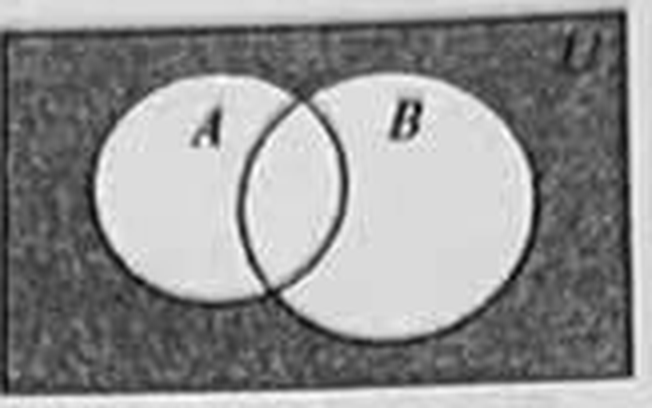
\includegraphics[width=0.30\textwidth]{figures/venn_AB_complement.png}
\end{center}

\ans{$\overline{A\cup B}$}

\ifanswer
\solbegin
\step{图中阴影部分在集合 $A$、$B$ 的外部，即在全集 $U$ 中但不属于 $A$、也不属于 $B$.}
\step{这正是 $A\cup B$ 在全集 $U$ 中的补集，故可表示为 $\overline{A\cup B}$（即 $\complement_U(A\cup B)$）.}
\solend

\fi

\item 设全集 $U=\R$，集合 $A=\{x\mid 2\leqslant x<5\}$，$B=\{x\mid 3<x<6\}$，则 $\overline{A}\cap B=$ \blankline[4.4em]（用区间表示）.

\ans{$[5,6)$}

\ifanswer
\solbegin
\step{在全集 $\R$ 中，$\overline{A}=(-\infty,2)\cup[5,+\infty)$.}
\step{又 $B=(3,6)$，取两集合的公共部分得 $\overline{A}\cap B=[5,6)$.}
\solend

\fi

\item 用反证法证明“$a,b\in\N$，$ab$ 可被 5 整除，那么 $a,b$ 中至少有一个能被 5 整除”时应假设 \blankline[4.4em].

\ans{$a,b$ 都不能被 5 整除}

\ifanswer
\solbegin
\step{反证法需假设结论的反面成立.}
\step{“$a,b$ 中至少有一个能被 5 整除”的反面是“$a,b$ 中没有一个能被 5 整除”，即 $a,b$ 都不能被 5 整除.}
\solend

\fi

\item 满足 $M\subseteq\{a_1,a_2,a_3,a_4,a_5\}$，且 $M\cap\{a_1,a_2,a_3\}=\{a_1,a_2\}$，则集合 $M$ 的个数是 \blankline[2.4em].

\ans{$4$}

\ifanswer
\solbegin
\step{由 $M\cap\{a_1,a_2,a_3\}=\{a_1,a_2\}$ 得 $a_1\in M$，$a_2\in M$，$a_3\notin M$.}
\step{又 $M\subseteq\{a_1,a_2,a_3,a_4,a_5\}$，所以 $a_4$、$a_5$ 可以属于 $M$，也可以不属于 $M$.}
\step{即 $M=\{a_1,a_2\}\cup S$，其中 $S\subseteq\{a_4,a_5\}$，共有 $2^2=4$ 个.}
\solend

\fi

\item 已知集合 $A=\{(x,y)\mid y=x^2\}$，$B=\left\{(x,y)\mid \dfrac{y-1}{x-1}=\dfrac{1}{2}\right\}$，则 $A\cap B=$ \blankline[5.2em].

\ans{$\left\{\left(-\dfrac{1}{2},\dfrac{1}{4}\right)\right\}$}

\ifanswer
\solbegin
\step{集合 $B$ 中的点满足 $y=\dfrac{1}{2}x+\dfrac{1}{2}$，且 $x\neq 1$.}
\step{代入 $y=x^2$ 得 $2x^2-x-1=0$，解得 $x=1$ 或 $x=-\dfrac{1}{2}$.}
\step{因为 $x\neq 1$，所以 $x=-\dfrac{1}{2}$，此时 $y=\dfrac{1}{4}$.}
\step{所以 $A\cap B=\left\{\left(-\dfrac{1}{2},\dfrac{1}{4}\right)\right\}$.}
\solend

\fi

\item 已知集合 $\{a,b,c\}=\{0,1,2\}$，且下列三个关系：①$a\neq 2$ ②$b=2$ ③$c\neq 0$ 有且只有一个正确，则 $100a+10b+c$ 等于 \blankline[2.4em].

\ans{$201$}

\ifanswer
\solbegin
\step{$a,b,c$ 是 $0,1,2$ 的一个排列，共 6 种情形，逐一检验三个关系的真假：}
\step{$(a,b,c)=(0,1,2)$：①真、②假、③真，两个正确，不合；$(0,2,1)$：三个都真，不合；}
\step{$(1,0,2)$：①真、②假、③真，两个正确，不合；$(1,2,0)$：①真、②真、③假，两个正确，不合；}
\step{$(2,0,1)$：①假、②假、③真，恰有一个正确，符合；$(2,1,0)$：三个都假，不合.}
\step{所以 $(a,b,c)=(2,0,1)$，$100a+10b+c=200+0+1=201$.}
\solend

\fi

\item “$x_1>3$ 且 $x_2>3$”是“$x_1+x_2>6$ 且 $x_1x_2>9$”的 \blankline[4.4em] 条件.（选填“充分非必要”，“必要非充分”，“充要”，“既非充分也非必要”）

\ans{充分非必要}

\ifanswer
\solbegin
\step{充分性：若 $x_1>3$ 且 $x_2>3$，则 $x_1+x_2>6$，且 $x_1x_2>9$，故充分性成立.}
\step{必要性：取 $x_1=2$、$x_2=5$，有 $x_1+x_2=7>6$、$x_1x_2=10>9$，但 $x_1>3$ 不成立，故必要性不成立.}
\step{所以应填“充分非必要”.}
\solend

\fi

% 注：第 11 题系 2010 年上海高考理科第 14 题的改写（原题要求选出 4 个子集，官方答案 36）。
%     原题官方解答明言「A、B 可以互换，即视为一种选法」，即**不计先后**计数；
%     按此口径本改写题的答案为 5。（原卷学生作答为 10，是把 A⊆B 与 B⊆A 重复计入。）
\item 在集合 $U=\{a,b,c,d\}$ 的子集中选出 2 个不同的子集，需同时满足以下两个条件：(1)$a,b$ 都要选出 (2)对选出的任意两个子集 $A$ 和 $B$，必有 $A\subseteq B$ 或 $B\subseteq A$，那么共有 \blankline[2.4em] 种不同的选法.

\ans{$5$}

\ifanswer
\solbegin
\step{由 (1) 知 $a,b$ 都要选出，即 $a,b$ 都属于所选的两个子集；由 (2) 知所选的两个子集必须可比.}
\step{含 $a,b$ 的子集只有 $\{a,b\}$、$\{a,b,c\}$、$\{a,b,d\}$、$\{a,b,c,d\}$ 共 4 个.}
\step{在这 4 个子集中取出两个不同的且可比的（一个包含另一个），只有下列 5 组：}
\step{$\{a,b\}\subset\{a,b,c\}$、$\{a,b\}\subset\{a,b,d\}$、$\{a,b\}\subset\{a,b,c,d\}$、$\{a,b,c\}\subset\{a,b,c,d\}$、$\{a,b,d\}\subset\{a,b,c,d\}$.}
\step{注意「选出 2 个子集」的选法\textbf{不计先后}：把这两个子集分别叫作 $A$、$B$ 只是给它们取个名字，$A\subseteq B$ 与 $B\subseteq A$ 说的是同一组子集，算同一种选法.}
\step{（本题由 2010 年上海高考理科第 14 题改写，原题要求选出 4 个子集，其官方答案 36 正是按「$A$、$B$ 可以互换，即视为一种选法」的不计先后口径计数.）}
\step{所以共有 5 种不同的选法.}
\solend

\fi

\end{enumerate}

\bigsec{二、选择题}

\begin{enumerate}
\setcounter{enumi}{11}

\item 已知 $M=(-\infty,\sqrt{3}]$，$a=\sqrt{3}$，则下列关系中正确的是（\quad）.

A. $a\subset M$\qquad B. $a\in M$\qquad C. $\{a\}\in M$\qquad D. $M\subset\{a\}$

\ans{B}

\ifanswer
\solbegin
\step{因为 $\sqrt{3}\leqslant\sqrt{3}$，所以 $a=\sqrt{3}\in M$，B 正确.}
\step{$a$ 是元素、$M$ 是集合，元素与集合之间用 $\in$ 表示，不能用 $\subset$，故 A、D 错误；}
\step{$\{a\}$ 是集合，集合与集合之间应是包含关系（且 $\{a\}\subseteq M$），不能用 $\in$，故 C 错误.}
\step{故选 B.}
\solend

\fi

% 注：原卷此处印作“已知集合{(x,y)|x^2+y^2≤3, x∈Z, y∈Z}”，集合未记作 A，
%     却设问“则 A 中的元素个数是”，显系漏排“A=”；本稿补上，其余照原卷。
\item 已知集合 $A=\{(x,y)\mid x^2+y^2\leqslant 3,\ x\in\Z,\ y\in\Z\}$，则 $A$ 中的元素个数是（\quad）.

A. $9$\qquad B. $8$\qquad C. $5$\qquad D. $4$

\ans{A}

\ifanswer
\solbegin
\step{逐一列举：$x=0$ 时 $y^2\leqslant 3$，$y=-1,0,1$，得 $(0,-1),(0,0),(0,1)$，共 3 个；}
\step{$x=\pm 1$ 时 $y^2\leqslant 2$，$y=-1,0,1$，各得 3 个，共 6 个（$x^2+y^2=2\leqslant 3$ 满足条件）；}
\step{$|x|\geqslant 2$ 时 $x^2\geqslant 4>3$，无解.}
\step{所以 $A$ 中元素个数为 $3+6=9$. 故选 A.}
\solend

\fi

\item 集合 $A=\{x\mid x=(2k-1)\pi,\ k\in\Z\}$ 与 $B=\{x\mid x=(4n\pm 1)\pi,\ n\in\Z\}$ 之间的关系是（\quad）.

A. $A\subset B$\qquad B. $B\subset A$\qquad C. $A=B$\qquad D. 不确定

\ans{C}

\ifanswer
\solbegin
\step{$A$ 由 $\pi$ 的一切奇数倍组成，即 $A=\{\cdots,-3\pi,-\pi,\pi,3\pi,\cdots\}$.}
\step{$B$ 中 $4n+1$ 与 $4n-1$ （$n\in\Z$）都是奇数，故 $B\subseteq A$；}
\step{反之，任一奇数除以 4 的余数只能是 1 或 3：形如 $4m+1$ 的奇数含于 $B$（取 $n=m$），形如 $4m+3=4(m+1)-1$ 的奇数也含于 $B$（取 $n=m+1$），所以 $A\subseteq B$.}
\step{于是 $A\subseteq B$ 且 $B\subseteq A$，即 $A=B$. 故选 C.}
\solend

\fi

\item 设 $T$ 是由正三角形 $P_1P_2P_3$ 边上及其内部的点构成的集合，点 $O$ 是 $\triangle P_1P_2P_3$ 的中心. 若集合 $S=\{P\mid P\in T,\ |PO|\leqslant|PO_i|,\ i=1,2,3\}$，（符号 $|AB|$ 表示平面上两点 $A,B$ 间的距离），则集合 $S$ 表示的平面区域是（\quad）.

A. 四边形区域；\qquad B. 三角形区域；\qquad C. 六边形区域；\qquad D. 五边形区域；

\ans{C}

\ifanswer
\solbegin
\step{$|PO|\leqslant|PO_i|$ 表示点 $P$ 到 $O$ 的距离不大于到顶点 $P_i$ 的距离，即 $P$ 落在线段 $OP_i$ 的垂直平分线靠 $O$ 的那一侧（含该线）.}
\step{对 $i=1,2,3$ 各有一条这样的直线，它们分别把三角形靠近 $P_1$、$P_2$、$P_3$ 的一个小角（三角形）截掉；}
\step{逐一直观验证可知这三条直线两两的交点都在三角形内部，三个角互不重叠，截去三个角后剩下的区域共有 6 条边.}
\step{所以集合 $S$ 表示的平面区域是六边形区域. 故选 C.}
\solend

\fi

\end{enumerate}

\bigsec{三、解答题}

\begin{enumerate}
\setcounter{enumi}{15}

\item（10 分，第 1 小问 5 分，第 2 小问 5 分）已知集合 $A=\{x\mid a\leqslant x\leqslant a+2\}$，集合 $B=\{x\mid x<-1\text{ 或 }x>5\}$，全集 $U=\R$.

\begin{enumerate}[label=(\arabic*)]
\item 若 $a=1$，求 $\overline{A}\cup B$；
\item 若 $A\subseteq B$，求实数 $a$ 的取值范围.
\end{enumerate}

\ans{（1）$(-\infty,1)\cup(3,+\infty)$；（2）$(-\infty,-3)\cup(5,+\infty)$}

\ifanswer
\solbegin
\stepm{(1)}{$a=1$ 时 $A=\{x\mid 1\leqslant x\leqslant 3\}=[1,3]$，则 $\overline{A}=(-\infty,1)\cup(3,+\infty)$.}
\step{又 $B=(-\infty,-1)\cup(5,+\infty)$，而 $B\subseteq\overline{A}$（因 $5>3$、$-1<1$），}
\step{所以 $\overline{A}\cup B=(-\infty,1)\cup(3,+\infty)$.}
\stepm{(2)}{因为 $a\leqslant a+2$，所以集合 $A=\{x\mid a\leqslant x\leqslant a+2\}$ 始终非空.}
\step{要使 $A\subseteq B$，只需 $A$ 与 $[-1,5]$ 没有公共点，即 $a+2<-1$ 或 $a>5$.}
\step{解得 $a<-3$ 或 $a>5$，所以实数 $a$ 的取值范围是 $(-\infty,-3)\cup(5,+\infty)$.}
\solend

\fi

\ansspace[10]

\item（10 分，第 1 小问 5 分，第 2 小问 5 分）已知 $A=\{x\mid x^2+x-2=0\}$，$B=\{x\mid x^2+ax+2a-4=0\}$.

\begin{enumerate}[label=(\arabic*)]
\item 若 $A=B$，求实数 $a$ 的值；
\item 若 $B\subseteq A$，求实数 $a$ 的值.
\end{enumerate}

\ans{（1）$a=1$；（2）$a=1$ 或 $a=4$}

\ifanswer
\solbegin
\stepm{(1)}{由 $x^2+x-2=0$ 解得 $x=1$ 或 $x=-2$，所以 $A=\{1,-2\}$.}
\step{由 $A=B$ 知 $1$、$-2$ 是方程 $x^2+ax+2a-4=0$ 的两根，由根与系数的关系得 $1+(-2)=-a$，所以 $a=1$；}
\step{此时 $2a-4=-2=1\times(-2)$，与两根之积相符，故 $a=1$.}
\stepm{(2)}{方程 $x^2+ax+2a-4=0$ 的判别式 $\Delta=a^2-4(2a-4)=(a-4)^2\geqslant 0$ 恒成立，所以集合 $B$ 不可能是空集.}
\step{由 $B\subseteq A$ 知 $B=\{1\}$ 或 $B=\{-2\}$ 或 $B=\{1,-2\}$.}
\step{若 $B=\{1\}$，则 $1$ 是二重根，$1+1=-a$ 且 $1\times 1=2a-4$，即 $a=-2$ 且 $a=\dfrac{5}{2}$，无解；}
\step{若 $B=\{-2\}$，则 $-2$ 是二重根，$(-2)+(-2)=-a$ 且 $(-2)\times(-2)=2a-4$，两式都给出 $a=4$，符合；}
\step{若 $B=\{1,-2\}$，则 $1+(-2)=-a$，得 $a=1$，此时 $2a-4=-2=1\times(-2)$，符合.}
\step{综上，$a=1$ 或 $a=4$.}
\solend

\fi

\ansspace[12]

\item（11 分，第 1 小问 3 分，第 2 小问 3 分，第 3 小问 5 分）已知非空数集 $S$ 满足：对任意给定的 $x,y\in S$（$x,y$ 可以相同），有 $x+y\in S$ 且 $x-y\in S$.

\begin{enumerate}[label=(\arabic*)]
\item 哪个数一定是 $S$ 中的元素?说明理由；
\item 若 $S$ 是有限集，求 $S$；
\item 若 $S$ 中最小的正数为 5，求 $S$.
\end{enumerate}

\ans{（1）$0$；（2）$S=\{0\}$；（3）$S=\{x\mid x=5a,\ a\in\Z\}$}

\ifanswer
\solbegin
\stepm{(1)}{$0$ 一定是 $S$ 中的元素. 理由：$S$ 非空，取 $x\in S$，在 $x-y\in S$ 中令 $y=x$（$x,y$ 可以相同），得 $x-x=0\in S$.}
\stepm{(2)}{若 $S$ 是有限集，则 $S=\{0\}$. 理由：取 $x\in S$ 且 $x\neq 0$，由 $x+y\in S$ 依次得 $2x=x+x\in S$，$3x=2x+x\in S$，$\cdots$，即 $kx\in S$（$k=1,2,3,\cdots$）；}
\step{这些数互不相同，与 $S$ 是有限集矛盾，所以 $S$ 中除 $0$ 外没有别的元素，即 $S=\{0\}$（此时 $0+0=0\in S$，$0-0=0\in S$，符合条件）.}
\stepm{(3)}{因为 $5\in S$，由 $x+y\in S$ 得 $5+5=10\in S$，$10+5=15\in S$，$\cdots$，故一切正整数倍的 $5$ 都在 $S$ 中；}
\step{又由 $x-y\in S$ 得 $5-5=0\in S$，$0-5=-5\in S$，$-5-5=-10\in S$，$\cdots$，故一切负整数倍的 $5$ 也都在 $S$ 中，即 $\{5a\mid a\in\Z\}\subseteq S$.}
\step{反之，任取 $s\in S$，由 $5\in S$ 及封闭性知 $s-5k\in S$（$k\in\Z$）；把 $s$ 写成 $s=5q+r$（$q\in\Z$，$0\leqslant r<5$），取 $k=q$ 得 $r=s-5q\in S$.}
\step{若 $r>0$，则 $S$ 中有比 $5$ 更小的正数 $r$，与“$S$ 中最小的正数为 5”矛盾，故只能 $r=0$，即 $s=5q$.}
\step{所以 $S=\{x\mid x=5a,\ a\in\Z\}$.}
\solend

\fi

\ansspace[12]

\end{enumerate}

\bigsec{附加题}

\begin{enumerate}
\setcounter{enumi}{18}

\item 已知集合 $A,B,C\subseteq\{1,2,3,\cdots,2024\}$，且 $A\subseteq B\subseteq C$，则有序集合组 $(A,B,C)$ 的个数是 \blankline[3.2em].

\ans{$4^{2024}$}

\ifanswer
\solbegin
\step{对 $U=\{1,2,\cdots,2024\}$ 中的每个元素，它与 $A,B,C$ 的关系只有四种可能：}
\step{在 $A,B,C$ 中都出现；不在 $A$ 中而在 $B,C$ 中出现；只在 $C$ 中出现；在三个集合中都不出现.}
\step{反过来，任取每个元素的一种归属方式，都恰好得到一个满足 $A\subseteq B\subseteq C$ 的有序集合组，故不同的组与不同的归属方式一一对应.}
\step{所以共有 $4\times 4\times\cdots\times 4=4^{2024}$ 个有序集合组.}
\solend

\fi

\item 已知集合 $M=\{1,2,\cdots,10\}$，对它的非空子集 $A$，将 $A$ 中的每个元素 $k$ 都乘以 $(-1)^k$ 再求和，如 $A=\{2,3,6\}$，可求得和为 $(-1)^2\times 2+(-1)^3\times 3+(-1)^6\times 6=5$. 试对 $M$ 的所有非空子集，求这些和的总和 \blankline[3.2em].

\ans{$2560$}

\ifanswer
\solbegin
\step{元素 $k$（$k=1,2,\cdots,10$）出现在 $M$ 的 $2^{9}$ 个非空子集中（其余 9 个元素任取）.}
\step{所以在所有非空子集的和中，$k$ 贡献的总量为 $2^{9}\times(-1)^k\cdot k=512\times(-1)^kk$.}
\step{于是这些和的总和为 $512\displaystyle\sum_{k=1}^{10}(-1)^kk=512\times(-1+2-3+4-5+6-7+8-9+10)=512\times 5=2560$.}
\solend

\fi

\item 设 $a_1,a_2,a_3,a_4$ 是 4 个有理数，使得 $\{a_ia_j\mid 1\leqslant i<j\leqslant 4\}=\left\{-24,-2,-\dfrac{3}{2},-\dfrac{1}{8},1,3\right\}$. 求 $a_1+a_2+a_3+a_4=$ \blankline[3.2em].

\ans{$\pm\dfrac{9}{4}$（两组解，和分别为 $-\dfrac{9}{4}$ 与 $\dfrac{9}{4}$）}

\ifanswer
\solbegin
\step{六个乘积中有 4 个负数、2 个正数. 设 4 个数中正数有 $p$ 个、负数有 $q$ 个（$p+q=4$），则异号的两数相乘得负数，其个数为 $pq$；由 $pq=4$ 得 $p=q=2$，即恰有 2 个正数、2 个负数.}
\step{把 4 个数的绝对值记作 $w,x,y,z>0$，则六个两两乘积的绝对值为 $24,2,\dfrac{3}{2},\dfrac{1}{8},1,3$；其中 $1$ 与 $3$ 来自两对同号的数，$24,2,\dfrac{3}{2},\dfrac{1}{8}$ 来自四对异号的数.}
\step{由 $(a_1a_2a_3a_4)^3=(-24)\times(-2)\times\left(-\dfrac{3}{2}\right)\times\left(-\dfrac{1}{8}\right)\times 1\times 3=27$ 得 $a_1a_2a_3a_4=3$，即去符号后 $wxyz=3$.}
\step{逐一检验可知 $w,x,y,z$ 只能是 $\left\{4,\dfrac{1}{4},6,\dfrac{1}{2}\right\}$：其中 $4\times\dfrac{1}{4}=1$、$6\times\dfrac{1}{2}=3$ 为同号两对的乘积，$4\times 6=24$、$4\times\dfrac{1}{2}=2$、$\dfrac{1}{4}\times 6=\dfrac{3}{2}$、$\dfrac{1}{4}\times\dfrac{1}{2}=\dfrac{1}{8}$ 为异号四对的乘积.}
\step{于是 $\left\{4,\dfrac{1}{4}\right\}$ 中的两个数同号、$\left\{6,\dfrac{1}{2}\right\}$ 中的两个数同号，且这两组异号，得两组解：}
\step{$4,\ \dfrac{1}{4},\ -6,\ -\dfrac{1}{2}$，和为 $-\dfrac{9}{4}$；\quad 或 \quad $6,\ \dfrac{1}{2},\ -4,\ -\dfrac{1}{4}$，和为 $\dfrac{9}{4}$.}
\step{两组解的六个乘积都恰为 $-24,-2,-\dfrac{3}{2},-\dfrac{1}{8},1,3$，与原卷所给集合相同.}
\step{所以 $a_1+a_2+a_3+a_4=\pm\dfrac{9}{4}$.}
\solend

\fi

\end{enumerate}

\end{document}
"
% 紧凑版：xelatex "\def\iscompact{1}% 高一16_大同中学_第二周周末练习1.tex —— 高一上数学「第二周周末练习1」（试卷版/答案版）
% 试卷版：xelatex 高一16_大同中学_第二周周末练习1.tex
% 答案版：xelatex "\def\isanswer{1}\input{高一16_大同中学_第二周周末练习1.tex}"
% 紧凑版：xelatex "\def\iscompact{1}\input{高一16_大同中学_第二周周末练习1.tex}"
%
% 原始材料为学生作业的手机翻拍照片（卷面为学生本人的**手写作答**，未见教师批改痕迹）。
% 试题文字照原卷录入；答案版给出的是**经核验的正确解答与解析**，与原卷手写答案的差异见 README。
%
% 与原卷的两处排版差异（均已在 README「说明」中交代）：
%   ① 原卷未印分节标题与分值，本稿按题型补「一、填空题 / 二、选择题 / 三、解答题」三节
%      （「附加题」原卷有印）；
%   ② 第 13 题原卷印作「已知集合{(x,y)|…}」，集合未记作 A 却被设问为「A 中的元素个数」，
%      显系漏排「A=」，本稿补上。

% 本篇的正文与家长拍照卷 `高一b_大同中学_第二周周末练习1（补）` **完全相同**——同一份作业，
% 试卷版/答案版也都是同一份源码编译而来；`高一b` 的 4 张原图另存于
% `原图/高一b_大同中学_第二周周末练习1（补）/`，本卷 `原图/` 下是同一组照片的副本。
% 经核对，这份作业就是公众号「魔都数学加油站」连载「27学年高一16——2026-2027年上海市大同中学
% 高一上周末作业2.1」的那一份：**题号与题干逐题一致**，只是公众号版略去了填空第 1、2 题，
% 故拍照卷反而是更完整的版本（对照关系见 README「与公众号连载号的对照表」）。
%
% 本卷的编号与连载号对齐（高一16），卷面标题因此**不带**「（补）」；标题里的「大同中学」为**本稿所加**
% （原卷标题只有作业名，校名只印在页眉「上海市大同…」）。带「（补）」的 `高一b` 保留为
% 拍照原件的转录本，两者内容一字不差。
%
% 一处与公众号讲评版的差异需留意：本卷第 11 题的答案按 2010 年上海高考理科第 14 题官方解答
% 「A、B 可以互换，即视为一种选法」的不计先后口径取 5，而公众号讲评版把它按有先后的 32 计数
% （该题学生原作答为 10）。取舍理由见该题下的 `%` 注。
\documentclass[a4paper,11pt]{article}
\usepackage{common}

\begin{document}

\examtitlest[3]{2026--2027 学年度大同中学高一上数学第二周周末练习1}{集合与常用逻辑用语}

\bigsec{一、填空题}

\begin{enumerate}

\item 用列举法表示集合 $\{x\mid -2<x\leqslant 2,\ x\in\Z\}=$ \blankline[2.4em].

\ans{$\{-1,0,1,2\}$}

\ifanswer
\solbegin
\step{集合中的元素是满足 $-2<x\leqslant 2$ 的整数，即 $-1$、$0$、$1$、$2$.}
\step{所以用列举法表示为 $\{-1,0,1,2\}$.}
\solend

\fi

\item 设集合 $A=\{1,a\}$，$B=\{1,a^2\}$，若 $A=B$，则实数 $a$ 的值为 \blankline[2.4em].

\ans{$a=0$}

\ifanswer
\solbegin
\step{由 $A=B$ 得 $a^2=a$，解得 $a=0$ 或 $a=1$.}
\step{当 $a=1$ 时，$A=\{1,1\}$，不符合集合元素的互异性，舍去；}
\step{当 $a=0$ 时，$A=\{1,0\}$，$B=\{1,0\}$，两集合相等，符合条件.}
\step{所以 $a=0$.}
\solend

\fi

\item 已知集合 $A=\{0,2,3,4,5\}$，$B=\{2,3,5,7\}$，$C=\{2,3,6\}$，则 $(A\cap B)\cup C=$ \blankline[4.4em].

\ans{$\{2,3,5,6\}$}

\ifanswer
\solbegin
\step{$A\cap B=\{0,2,3,4,5\}\cap\{2,3,5,7\}=\{2,3,5\}$.}
\step{所以 $(A\cap B)\cup C=\{2,3,5\}\cup\{2,3,6\}=\{2,3,5,6\}$.}
\solend

\fi

\item 设全集为 $U$，用集合 $A,B$ 的交、并或补集符号表示图中的阴影部分是 \blankline[4.4em].

\begin{center}
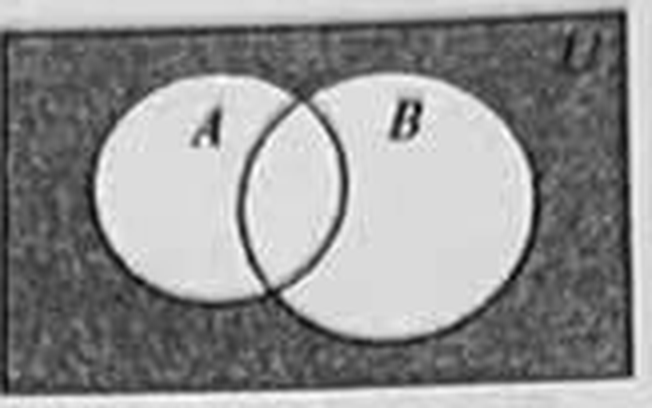
\includegraphics[width=0.30\textwidth]{figures/venn_AB_complement.png}
\end{center}

\ans{$\overline{A\cup B}$}

\ifanswer
\solbegin
\step{图中阴影部分在集合 $A$、$B$ 的外部，即在全集 $U$ 中但不属于 $A$、也不属于 $B$.}
\step{这正是 $A\cup B$ 在全集 $U$ 中的补集，故可表示为 $\overline{A\cup B}$（即 $\complement_U(A\cup B)$）.}
\solend

\fi

\item 设全集 $U=\R$，集合 $A=\{x\mid 2\leqslant x<5\}$，$B=\{x\mid 3<x<6\}$，则 $\overline{A}\cap B=$ \blankline[4.4em]（用区间表示）.

\ans{$[5,6)$}

\ifanswer
\solbegin
\step{在全集 $\R$ 中，$\overline{A}=(-\infty,2)\cup[5,+\infty)$.}
\step{又 $B=(3,6)$，取两集合的公共部分得 $\overline{A}\cap B=[5,6)$.}
\solend

\fi

\item 用反证法证明“$a,b\in\N$，$ab$ 可被 5 整除，那么 $a,b$ 中至少有一个能被 5 整除”时应假设 \blankline[4.4em].

\ans{$a,b$ 都不能被 5 整除}

\ifanswer
\solbegin
\step{反证法需假设结论的反面成立.}
\step{“$a,b$ 中至少有一个能被 5 整除”的反面是“$a,b$ 中没有一个能被 5 整除”，即 $a,b$ 都不能被 5 整除.}
\solend

\fi

\item 满足 $M\subseteq\{a_1,a_2,a_3,a_4,a_5\}$，且 $M\cap\{a_1,a_2,a_3\}=\{a_1,a_2\}$，则集合 $M$ 的个数是 \blankline[2.4em].

\ans{$4$}

\ifanswer
\solbegin
\step{由 $M\cap\{a_1,a_2,a_3\}=\{a_1,a_2\}$ 得 $a_1\in M$，$a_2\in M$，$a_3\notin M$.}
\step{又 $M\subseteq\{a_1,a_2,a_3,a_4,a_5\}$，所以 $a_4$、$a_5$ 可以属于 $M$，也可以不属于 $M$.}
\step{即 $M=\{a_1,a_2\}\cup S$，其中 $S\subseteq\{a_4,a_5\}$，共有 $2^2=4$ 个.}
\solend

\fi

\item 已知集合 $A=\{(x,y)\mid y=x^2\}$，$B=\left\{(x,y)\mid \dfrac{y-1}{x-1}=\dfrac{1}{2}\right\}$，则 $A\cap B=$ \blankline[5.2em].

\ans{$\left\{\left(-\dfrac{1}{2},\dfrac{1}{4}\right)\right\}$}

\ifanswer
\solbegin
\step{集合 $B$ 中的点满足 $y=\dfrac{1}{2}x+\dfrac{1}{2}$，且 $x\neq 1$.}
\step{代入 $y=x^2$ 得 $2x^2-x-1=0$，解得 $x=1$ 或 $x=-\dfrac{1}{2}$.}
\step{因为 $x\neq 1$，所以 $x=-\dfrac{1}{2}$，此时 $y=\dfrac{1}{4}$.}
\step{所以 $A\cap B=\left\{\left(-\dfrac{1}{2},\dfrac{1}{4}\right)\right\}$.}
\solend

\fi

\item 已知集合 $\{a,b,c\}=\{0,1,2\}$，且下列三个关系：①$a\neq 2$ ②$b=2$ ③$c\neq 0$ 有且只有一个正确，则 $100a+10b+c$ 等于 \blankline[2.4em].

\ans{$201$}

\ifanswer
\solbegin
\step{$a,b,c$ 是 $0,1,2$ 的一个排列，共 6 种情形，逐一检验三个关系的真假：}
\step{$(a,b,c)=(0,1,2)$：①真、②假、③真，两个正确，不合；$(0,2,1)$：三个都真，不合；}
\step{$(1,0,2)$：①真、②假、③真，两个正确，不合；$(1,2,0)$：①真、②真、③假，两个正确，不合；}
\step{$(2,0,1)$：①假、②假、③真，恰有一个正确，符合；$(2,1,0)$：三个都假，不合.}
\step{所以 $(a,b,c)=(2,0,1)$，$100a+10b+c=200+0+1=201$.}
\solend

\fi

\item “$x_1>3$ 且 $x_2>3$”是“$x_1+x_2>6$ 且 $x_1x_2>9$”的 \blankline[4.4em] 条件.（选填“充分非必要”，“必要非充分”，“充要”，“既非充分也非必要”）

\ans{充分非必要}

\ifanswer
\solbegin
\step{充分性：若 $x_1>3$ 且 $x_2>3$，则 $x_1+x_2>6$，且 $x_1x_2>9$，故充分性成立.}
\step{必要性：取 $x_1=2$、$x_2=5$，有 $x_1+x_2=7>6$、$x_1x_2=10>9$，但 $x_1>3$ 不成立，故必要性不成立.}
\step{所以应填“充分非必要”.}
\solend

\fi

% 注：第 11 题系 2010 年上海高考理科第 14 题的改写（原题要求选出 4 个子集，官方答案 36）。
%     原题官方解答明言「A、B 可以互换，即视为一种选法」，即**不计先后**计数；
%     按此口径本改写题的答案为 5。（原卷学生作答为 10，是把 A⊆B 与 B⊆A 重复计入。）
\item 在集合 $U=\{a,b,c,d\}$ 的子集中选出 2 个不同的子集，需同时满足以下两个条件：(1)$a,b$ 都要选出 (2)对选出的任意两个子集 $A$ 和 $B$，必有 $A\subseteq B$ 或 $B\subseteq A$，那么共有 \blankline[2.4em] 种不同的选法.

\ans{$5$}

\ifanswer
\solbegin
\step{由 (1) 知 $a,b$ 都要选出，即 $a,b$ 都属于所选的两个子集；由 (2) 知所选的两个子集必须可比.}
\step{含 $a,b$ 的子集只有 $\{a,b\}$、$\{a,b,c\}$、$\{a,b,d\}$、$\{a,b,c,d\}$ 共 4 个.}
\step{在这 4 个子集中取出两个不同的且可比的（一个包含另一个），只有下列 5 组：}
\step{$\{a,b\}\subset\{a,b,c\}$、$\{a,b\}\subset\{a,b,d\}$、$\{a,b\}\subset\{a,b,c,d\}$、$\{a,b,c\}\subset\{a,b,c,d\}$、$\{a,b,d\}\subset\{a,b,c,d\}$.}
\step{注意「选出 2 个子集」的选法\textbf{不计先后}：把这两个子集分别叫作 $A$、$B$ 只是给它们取个名字，$A\subseteq B$ 与 $B\subseteq A$ 说的是同一组子集，算同一种选法.}
\step{（本题由 2010 年上海高考理科第 14 题改写，原题要求选出 4 个子集，其官方答案 36 正是按「$A$、$B$ 可以互换，即视为一种选法」的不计先后口径计数.）}
\step{所以共有 5 种不同的选法.}
\solend

\fi

\end{enumerate}

\bigsec{二、选择题}

\begin{enumerate}
\setcounter{enumi}{11}

\item 已知 $M=(-\infty,\sqrt{3}]$，$a=\sqrt{3}$，则下列关系中正确的是（\quad）.

A. $a\subset M$\qquad B. $a\in M$\qquad C. $\{a\}\in M$\qquad D. $M\subset\{a\}$

\ans{B}

\ifanswer
\solbegin
\step{因为 $\sqrt{3}\leqslant\sqrt{3}$，所以 $a=\sqrt{3}\in M$，B 正确.}
\step{$a$ 是元素、$M$ 是集合，元素与集合之间用 $\in$ 表示，不能用 $\subset$，故 A、D 错误；}
\step{$\{a\}$ 是集合，集合与集合之间应是包含关系（且 $\{a\}\subseteq M$），不能用 $\in$，故 C 错误.}
\step{故选 B.}
\solend

\fi

% 注：原卷此处印作“已知集合{(x,y)|x^2+y^2≤3, x∈Z, y∈Z}”，集合未记作 A，
%     却设问“则 A 中的元素个数是”，显系漏排“A=”；本稿补上，其余照原卷。
\item 已知集合 $A=\{(x,y)\mid x^2+y^2\leqslant 3,\ x\in\Z,\ y\in\Z\}$，则 $A$ 中的元素个数是（\quad）.

A. $9$\qquad B. $8$\qquad C. $5$\qquad D. $4$

\ans{A}

\ifanswer
\solbegin
\step{逐一列举：$x=0$ 时 $y^2\leqslant 3$，$y=-1,0,1$，得 $(0,-1),(0,0),(0,1)$，共 3 个；}
\step{$x=\pm 1$ 时 $y^2\leqslant 2$，$y=-1,0,1$，各得 3 个，共 6 个（$x^2+y^2=2\leqslant 3$ 满足条件）；}
\step{$|x|\geqslant 2$ 时 $x^2\geqslant 4>3$，无解.}
\step{所以 $A$ 中元素个数为 $3+6=9$. 故选 A.}
\solend

\fi

\item 集合 $A=\{x\mid x=(2k-1)\pi,\ k\in\Z\}$ 与 $B=\{x\mid x=(4n\pm 1)\pi,\ n\in\Z\}$ 之间的关系是（\quad）.

A. $A\subset B$\qquad B. $B\subset A$\qquad C. $A=B$\qquad D. 不确定

\ans{C}

\ifanswer
\solbegin
\step{$A$ 由 $\pi$ 的一切奇数倍组成，即 $A=\{\cdots,-3\pi,-\pi,\pi,3\pi,\cdots\}$.}
\step{$B$ 中 $4n+1$ 与 $4n-1$ （$n\in\Z$）都是奇数，故 $B\subseteq A$；}
\step{反之，任一奇数除以 4 的余数只能是 1 或 3：形如 $4m+1$ 的奇数含于 $B$（取 $n=m$），形如 $4m+3=4(m+1)-1$ 的奇数也含于 $B$（取 $n=m+1$），所以 $A\subseteq B$.}
\step{于是 $A\subseteq B$ 且 $B\subseteq A$，即 $A=B$. 故选 C.}
\solend

\fi

\item 设 $T$ 是由正三角形 $P_1P_2P_3$ 边上及其内部的点构成的集合，点 $O$ 是 $\triangle P_1P_2P_3$ 的中心. 若集合 $S=\{P\mid P\in T,\ |PO|\leqslant|PO_i|,\ i=1,2,3\}$，（符号 $|AB|$ 表示平面上两点 $A,B$ 间的距离），则集合 $S$ 表示的平面区域是（\quad）.

A. 四边形区域；\qquad B. 三角形区域；\qquad C. 六边形区域；\qquad D. 五边形区域；

\ans{C}

\ifanswer
\solbegin
\step{$|PO|\leqslant|PO_i|$ 表示点 $P$ 到 $O$ 的距离不大于到顶点 $P_i$ 的距离，即 $P$ 落在线段 $OP_i$ 的垂直平分线靠 $O$ 的那一侧（含该线）.}
\step{对 $i=1,2,3$ 各有一条这样的直线，它们分别把三角形靠近 $P_1$、$P_2$、$P_3$ 的一个小角（三角形）截掉；}
\step{逐一直观验证可知这三条直线两两的交点都在三角形内部，三个角互不重叠，截去三个角后剩下的区域共有 6 条边.}
\step{所以集合 $S$ 表示的平面区域是六边形区域. 故选 C.}
\solend

\fi

\end{enumerate}

\bigsec{三、解答题}

\begin{enumerate}
\setcounter{enumi}{15}

\item（10 分，第 1 小问 5 分，第 2 小问 5 分）已知集合 $A=\{x\mid a\leqslant x\leqslant a+2\}$，集合 $B=\{x\mid x<-1\text{ 或 }x>5\}$，全集 $U=\R$.

\begin{enumerate}[label=(\arabic*)]
\item 若 $a=1$，求 $\overline{A}\cup B$；
\item 若 $A\subseteq B$，求实数 $a$ 的取值范围.
\end{enumerate}

\ans{（1）$(-\infty,1)\cup(3,+\infty)$；（2）$(-\infty,-3)\cup(5,+\infty)$}

\ifanswer
\solbegin
\stepm{(1)}{$a=1$ 时 $A=\{x\mid 1\leqslant x\leqslant 3\}=[1,3]$，则 $\overline{A}=(-\infty,1)\cup(3,+\infty)$.}
\step{又 $B=(-\infty,-1)\cup(5,+\infty)$，而 $B\subseteq\overline{A}$（因 $5>3$、$-1<1$），}
\step{所以 $\overline{A}\cup B=(-\infty,1)\cup(3,+\infty)$.}
\stepm{(2)}{因为 $a\leqslant a+2$，所以集合 $A=\{x\mid a\leqslant x\leqslant a+2\}$ 始终非空.}
\step{要使 $A\subseteq B$，只需 $A$ 与 $[-1,5]$ 没有公共点，即 $a+2<-1$ 或 $a>5$.}
\step{解得 $a<-3$ 或 $a>5$，所以实数 $a$ 的取值范围是 $(-\infty,-3)\cup(5,+\infty)$.}
\solend

\fi

\ansspace[10]

\item（10 分，第 1 小问 5 分，第 2 小问 5 分）已知 $A=\{x\mid x^2+x-2=0\}$，$B=\{x\mid x^2+ax+2a-4=0\}$.

\begin{enumerate}[label=(\arabic*)]
\item 若 $A=B$，求实数 $a$ 的值；
\item 若 $B\subseteq A$，求实数 $a$ 的值.
\end{enumerate}

\ans{（1）$a=1$；（2）$a=1$ 或 $a=4$}

\ifanswer
\solbegin
\stepm{(1)}{由 $x^2+x-2=0$ 解得 $x=1$ 或 $x=-2$，所以 $A=\{1,-2\}$.}
\step{由 $A=B$ 知 $1$、$-2$ 是方程 $x^2+ax+2a-4=0$ 的两根，由根与系数的关系得 $1+(-2)=-a$，所以 $a=1$；}
\step{此时 $2a-4=-2=1\times(-2)$，与两根之积相符，故 $a=1$.}
\stepm{(2)}{方程 $x^2+ax+2a-4=0$ 的判别式 $\Delta=a^2-4(2a-4)=(a-4)^2\geqslant 0$ 恒成立，所以集合 $B$ 不可能是空集.}
\step{由 $B\subseteq A$ 知 $B=\{1\}$ 或 $B=\{-2\}$ 或 $B=\{1,-2\}$.}
\step{若 $B=\{1\}$，则 $1$ 是二重根，$1+1=-a$ 且 $1\times 1=2a-4$，即 $a=-2$ 且 $a=\dfrac{5}{2}$，无解；}
\step{若 $B=\{-2\}$，则 $-2$ 是二重根，$(-2)+(-2)=-a$ 且 $(-2)\times(-2)=2a-4$，两式都给出 $a=4$，符合；}
\step{若 $B=\{1,-2\}$，则 $1+(-2)=-a$，得 $a=1$，此时 $2a-4=-2=1\times(-2)$，符合.}
\step{综上，$a=1$ 或 $a=4$.}
\solend

\fi

\ansspace[12]

\item（11 分，第 1 小问 3 分，第 2 小问 3 分，第 3 小问 5 分）已知非空数集 $S$ 满足：对任意给定的 $x,y\in S$（$x,y$ 可以相同），有 $x+y\in S$ 且 $x-y\in S$.

\begin{enumerate}[label=(\arabic*)]
\item 哪个数一定是 $S$ 中的元素?说明理由；
\item 若 $S$ 是有限集，求 $S$；
\item 若 $S$ 中最小的正数为 5，求 $S$.
\end{enumerate}

\ans{（1）$0$；（2）$S=\{0\}$；（3）$S=\{x\mid x=5a,\ a\in\Z\}$}

\ifanswer
\solbegin
\stepm{(1)}{$0$ 一定是 $S$ 中的元素. 理由：$S$ 非空，取 $x\in S$，在 $x-y\in S$ 中令 $y=x$（$x,y$ 可以相同），得 $x-x=0\in S$.}
\stepm{(2)}{若 $S$ 是有限集，则 $S=\{0\}$. 理由：取 $x\in S$ 且 $x\neq 0$，由 $x+y\in S$ 依次得 $2x=x+x\in S$，$3x=2x+x\in S$，$\cdots$，即 $kx\in S$（$k=1,2,3,\cdots$）；}
\step{这些数互不相同，与 $S$ 是有限集矛盾，所以 $S$ 中除 $0$ 外没有别的元素，即 $S=\{0\}$（此时 $0+0=0\in S$，$0-0=0\in S$，符合条件）.}
\stepm{(3)}{因为 $5\in S$，由 $x+y\in S$ 得 $5+5=10\in S$，$10+5=15\in S$，$\cdots$，故一切正整数倍的 $5$ 都在 $S$ 中；}
\step{又由 $x-y\in S$ 得 $5-5=0\in S$，$0-5=-5\in S$，$-5-5=-10\in S$，$\cdots$，故一切负整数倍的 $5$ 也都在 $S$ 中，即 $\{5a\mid a\in\Z\}\subseteq S$.}
\step{反之，任取 $s\in S$，由 $5\in S$ 及封闭性知 $s-5k\in S$（$k\in\Z$）；把 $s$ 写成 $s=5q+r$（$q\in\Z$，$0\leqslant r<5$），取 $k=q$ 得 $r=s-5q\in S$.}
\step{若 $r>0$，则 $S$ 中有比 $5$ 更小的正数 $r$，与“$S$ 中最小的正数为 5”矛盾，故只能 $r=0$，即 $s=5q$.}
\step{所以 $S=\{x\mid x=5a,\ a\in\Z\}$.}
\solend

\fi

\ansspace[12]

\end{enumerate}

\bigsec{附加题}

\begin{enumerate}
\setcounter{enumi}{18}

\item 已知集合 $A,B,C\subseteq\{1,2,3,\cdots,2024\}$，且 $A\subseteq B\subseteq C$，则有序集合组 $(A,B,C)$ 的个数是 \blankline[3.2em].

\ans{$4^{2024}$}

\ifanswer
\solbegin
\step{对 $U=\{1,2,\cdots,2024\}$ 中的每个元素，它与 $A,B,C$ 的关系只有四种可能：}
\step{在 $A,B,C$ 中都出现；不在 $A$ 中而在 $B,C$ 中出现；只在 $C$ 中出现；在三个集合中都不出现.}
\step{反过来，任取每个元素的一种归属方式，都恰好得到一个满足 $A\subseteq B\subseteq C$ 的有序集合组，故不同的组与不同的归属方式一一对应.}
\step{所以共有 $4\times 4\times\cdots\times 4=4^{2024}$ 个有序集合组.}
\solend

\fi

\item 已知集合 $M=\{1,2,\cdots,10\}$，对它的非空子集 $A$，将 $A$ 中的每个元素 $k$ 都乘以 $(-1)^k$ 再求和，如 $A=\{2,3,6\}$，可求得和为 $(-1)^2\times 2+(-1)^3\times 3+(-1)^6\times 6=5$. 试对 $M$ 的所有非空子集，求这些和的总和 \blankline[3.2em].

\ans{$2560$}

\ifanswer
\solbegin
\step{元素 $k$（$k=1,2,\cdots,10$）出现在 $M$ 的 $2^{9}$ 个非空子集中（其余 9 个元素任取）.}
\step{所以在所有非空子集的和中，$k$ 贡献的总量为 $2^{9}\times(-1)^k\cdot k=512\times(-1)^kk$.}
\step{于是这些和的总和为 $512\displaystyle\sum_{k=1}^{10}(-1)^kk=512\times(-1+2-3+4-5+6-7+8-9+10)=512\times 5=2560$.}
\solend

\fi

\item 设 $a_1,a_2,a_3,a_4$ 是 4 个有理数，使得 $\{a_ia_j\mid 1\leqslant i<j\leqslant 4\}=\left\{-24,-2,-\dfrac{3}{2},-\dfrac{1}{8},1,3\right\}$. 求 $a_1+a_2+a_3+a_4=$ \blankline[3.2em].

\ans{$\pm\dfrac{9}{4}$（两组解，和分别为 $-\dfrac{9}{4}$ 与 $\dfrac{9}{4}$）}

\ifanswer
\solbegin
\step{六个乘积中有 4 个负数、2 个正数. 设 4 个数中正数有 $p$ 个、负数有 $q$ 个（$p+q=4$），则异号的两数相乘得负数，其个数为 $pq$；由 $pq=4$ 得 $p=q=2$，即恰有 2 个正数、2 个负数.}
\step{把 4 个数的绝对值记作 $w,x,y,z>0$，则六个两两乘积的绝对值为 $24,2,\dfrac{3}{2},\dfrac{1}{8},1,3$；其中 $1$ 与 $3$ 来自两对同号的数，$24,2,\dfrac{3}{2},\dfrac{1}{8}$ 来自四对异号的数.}
\step{由 $(a_1a_2a_3a_4)^3=(-24)\times(-2)\times\left(-\dfrac{3}{2}\right)\times\left(-\dfrac{1}{8}\right)\times 1\times 3=27$ 得 $a_1a_2a_3a_4=3$，即去符号后 $wxyz=3$.}
\step{逐一检验可知 $w,x,y,z$ 只能是 $\left\{4,\dfrac{1}{4},6,\dfrac{1}{2}\right\}$：其中 $4\times\dfrac{1}{4}=1$、$6\times\dfrac{1}{2}=3$ 为同号两对的乘积，$4\times 6=24$、$4\times\dfrac{1}{2}=2$、$\dfrac{1}{4}\times 6=\dfrac{3}{2}$、$\dfrac{1}{4}\times\dfrac{1}{2}=\dfrac{1}{8}$ 为异号四对的乘积.}
\step{于是 $\left\{4,\dfrac{1}{4}\right\}$ 中的两个数同号、$\left\{6,\dfrac{1}{2}\right\}$ 中的两个数同号，且这两组异号，得两组解：}
\step{$4,\ \dfrac{1}{4},\ -6,\ -\dfrac{1}{2}$，和为 $-\dfrac{9}{4}$；\quad 或 \quad $6,\ \dfrac{1}{2},\ -4,\ -\dfrac{1}{4}$，和为 $\dfrac{9}{4}$.}
\step{两组解的六个乘积都恰为 $-24,-2,-\dfrac{3}{2},-\dfrac{1}{8},1,3$，与原卷所给集合相同.}
\step{所以 $a_1+a_2+a_3+a_4=\pm\dfrac{9}{4}$.}
\solend

\fi

\end{enumerate}

\end{document}
"
%
% 原始材料为学生作业的手机翻拍照片（卷面为学生本人的**手写作答**，未见教师批改痕迹）。
% 试题文字照原卷录入；答案版给出的是**经核验的正确解答与解析**，与原卷手写答案的差异见 README。
%
% 与原卷的两处排版差异（均已在 README「说明」中交代）：
%   ① 原卷未印分节标题与分值，本稿按题型补「一、填空题 / 二、选择题 / 三、解答题」三节
%      （「附加题」原卷有印）；
%   ② 第 13 题原卷印作「已知集合{(x,y)|…}」，集合未记作 A 却被设问为「A 中的元素个数」，
%      显系漏排「A=」，本稿补上。

% 本篇的正文与家长拍照卷 `高一b_大同中学_第二周周末练习1（补）` **完全相同**——同一份作业，
% 试卷版/答案版也都是同一份源码编译而来；`高一b` 的 4 张原图另存于
% `原图/高一b_大同中学_第二周周末练习1（补）/`，本卷 `原图/` 下是同一组照片的副本。
% 经核对，这份作业就是公众号「魔都数学加油站」连载「27学年高一16——2026-2027年上海市大同中学
% 高一上周末作业2.1」的那一份：**题号与题干逐题一致**，只是公众号版略去了填空第 1、2 题，
% 故拍照卷反而是更完整的版本（对照关系见 README「与公众号连载号的对照表」）。
%
% 本卷的编号与连载号对齐（高一16），卷面标题因此**不带**「（补）」；标题里的「大同中学」为**本稿所加**
% （原卷标题只有作业名，校名只印在页眉「上海市大同…」）。带「（补）」的 `高一b` 保留为
% 拍照原件的转录本，两者内容一字不差。
%
% 一处与公众号讲评版的差异需留意：本卷第 11 题的答案按 2010 年上海高考理科第 14 题官方解答
% 「A、B 可以互换，即视为一种选法」的不计先后口径取 5，而公众号讲评版把它按有先后的 32 计数
% （该题学生原作答为 10）。取舍理由见该题下的 `%` 注。
\documentclass[a4paper,11pt]{article}
\usepackage{common}

\begin{document}

\examtitlest[3]{2026--2027 学年度大同中学高一上数学第二周周末练习1}{集合与常用逻辑用语}

\bigsec{一、填空题}

\begin{enumerate}

\item 用列举法表示集合 $\{x\mid -2<x\leqslant 2,\ x\in\Z\}=$ \blankline[2.4em].

\ans{$\{-1,0,1,2\}$}

\ifanswer
\solbegin
\step{集合中的元素是满足 $-2<x\leqslant 2$ 的整数，即 $-1$、$0$、$1$、$2$.}
\step{所以用列举法表示为 $\{-1,0,1,2\}$.}
\solend

\fi

\item 设集合 $A=\{1,a\}$，$B=\{1,a^2\}$，若 $A=B$，则实数 $a$ 的值为 \blankline[2.4em].

\ans{$a=0$}

\ifanswer
\solbegin
\step{由 $A=B$ 得 $a^2=a$，解得 $a=0$ 或 $a=1$.}
\step{当 $a=1$ 时，$A=\{1,1\}$，不符合集合元素的互异性，舍去；}
\step{当 $a=0$ 时，$A=\{1,0\}$，$B=\{1,0\}$，两集合相等，符合条件.}
\step{所以 $a=0$.}
\solend

\fi

\item 已知集合 $A=\{0,2,3,4,5\}$，$B=\{2,3,5,7\}$，$C=\{2,3,6\}$，则 $(A\cap B)\cup C=$ \blankline[4.4em].

\ans{$\{2,3,5,6\}$}

\ifanswer
\solbegin
\step{$A\cap B=\{0,2,3,4,5\}\cap\{2,3,5,7\}=\{2,3,5\}$.}
\step{所以 $(A\cap B)\cup C=\{2,3,5\}\cup\{2,3,6\}=\{2,3,5,6\}$.}
\solend

\fi

\item 设全集为 $U$，用集合 $A,B$ 的交、并或补集符号表示图中的阴影部分是 \blankline[4.4em].

\begin{center}
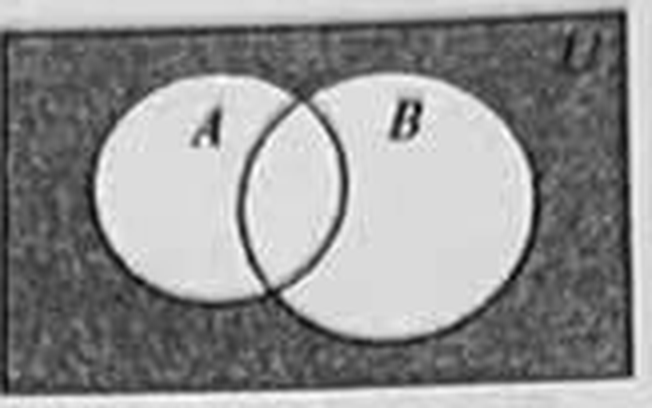
\includegraphics[width=0.30\textwidth]{figures/venn_AB_complement.png}
\end{center}

\ans{$\overline{A\cup B}$}

\ifanswer
\solbegin
\step{图中阴影部分在集合 $A$、$B$ 的外部，即在全集 $U$ 中但不属于 $A$、也不属于 $B$.}
\step{这正是 $A\cup B$ 在全集 $U$ 中的补集，故可表示为 $\overline{A\cup B}$（即 $\complement_U(A\cup B)$）.}
\solend

\fi

\item 设全集 $U=\R$，集合 $A=\{x\mid 2\leqslant x<5\}$，$B=\{x\mid 3<x<6\}$，则 $\overline{A}\cap B=$ \blankline[4.4em]（用区间表示）.

\ans{$[5,6)$}

\ifanswer
\solbegin
\step{在全集 $\R$ 中，$\overline{A}=(-\infty,2)\cup[5,+\infty)$.}
\step{又 $B=(3,6)$，取两集合的公共部分得 $\overline{A}\cap B=[5,6)$.}
\solend

\fi

\item 用反证法证明“$a,b\in\N$，$ab$ 可被 5 整除，那么 $a,b$ 中至少有一个能被 5 整除”时应假设 \blankline[4.4em].

\ans{$a,b$ 都不能被 5 整除}

\ifanswer
\solbegin
\step{反证法需假设结论的反面成立.}
\step{“$a,b$ 中至少有一个能被 5 整除”的反面是“$a,b$ 中没有一个能被 5 整除”，即 $a,b$ 都不能被 5 整除.}
\solend

\fi

\item 满足 $M\subseteq\{a_1,a_2,a_3,a_4,a_5\}$，且 $M\cap\{a_1,a_2,a_3\}=\{a_1,a_2\}$，则集合 $M$ 的个数是 \blankline[2.4em].

\ans{$4$}

\ifanswer
\solbegin
\step{由 $M\cap\{a_1,a_2,a_3\}=\{a_1,a_2\}$ 得 $a_1\in M$，$a_2\in M$，$a_3\notin M$.}
\step{又 $M\subseteq\{a_1,a_2,a_3,a_4,a_5\}$，所以 $a_4$、$a_5$ 可以属于 $M$，也可以不属于 $M$.}
\step{即 $M=\{a_1,a_2\}\cup S$，其中 $S\subseteq\{a_4,a_5\}$，共有 $2^2=4$ 个.}
\solend

\fi

\item 已知集合 $A=\{(x,y)\mid y=x^2\}$，$B=\left\{(x,y)\mid \dfrac{y-1}{x-1}=\dfrac{1}{2}\right\}$，则 $A\cap B=$ \blankline[5.2em].

\ans{$\left\{\left(-\dfrac{1}{2},\dfrac{1}{4}\right)\right\}$}

\ifanswer
\solbegin
\step{集合 $B$ 中的点满足 $y=\dfrac{1}{2}x+\dfrac{1}{2}$，且 $x\neq 1$.}
\step{代入 $y=x^2$ 得 $2x^2-x-1=0$，解得 $x=1$ 或 $x=-\dfrac{1}{2}$.}
\step{因为 $x\neq 1$，所以 $x=-\dfrac{1}{2}$，此时 $y=\dfrac{1}{4}$.}
\step{所以 $A\cap B=\left\{\left(-\dfrac{1}{2},\dfrac{1}{4}\right)\right\}$.}
\solend

\fi

\item 已知集合 $\{a,b,c\}=\{0,1,2\}$，且下列三个关系：①$a\neq 2$ ②$b=2$ ③$c\neq 0$ 有且只有一个正确，则 $100a+10b+c$ 等于 \blankline[2.4em].

\ans{$201$}

\ifanswer
\solbegin
\step{$a,b,c$ 是 $0,1,2$ 的一个排列，共 6 种情形，逐一检验三个关系的真假：}
\step{$(a,b,c)=(0,1,2)$：①真、②假、③真，两个正确，不合；$(0,2,1)$：三个都真，不合；}
\step{$(1,0,2)$：①真、②假、③真，两个正确，不合；$(1,2,0)$：①真、②真、③假，两个正确，不合；}
\step{$(2,0,1)$：①假、②假、③真，恰有一个正确，符合；$(2,1,0)$：三个都假，不合.}
\step{所以 $(a,b,c)=(2,0,1)$，$100a+10b+c=200+0+1=201$.}
\solend

\fi

\item “$x_1>3$ 且 $x_2>3$”是“$x_1+x_2>6$ 且 $x_1x_2>9$”的 \blankline[4.4em] 条件.（选填“充分非必要”，“必要非充分”，“充要”，“既非充分也非必要”）

\ans{充分非必要}

\ifanswer
\solbegin
\step{充分性：若 $x_1>3$ 且 $x_2>3$，则 $x_1+x_2>6$，且 $x_1x_2>9$，故充分性成立.}
\step{必要性：取 $x_1=2$、$x_2=5$，有 $x_1+x_2=7>6$、$x_1x_2=10>9$，但 $x_1>3$ 不成立，故必要性不成立.}
\step{所以应填“充分非必要”.}
\solend

\fi

% 注：第 11 题系 2010 年上海高考理科第 14 题的改写（原题要求选出 4 个子集，官方答案 36）。
%     原题官方解答明言「A、B 可以互换，即视为一种选法」，即**不计先后**计数；
%     按此口径本改写题的答案为 5。（原卷学生作答为 10，是把 A⊆B 与 B⊆A 重复计入。）
\item 在集合 $U=\{a,b,c,d\}$ 的子集中选出 2 个不同的子集，需同时满足以下两个条件：(1)$a,b$ 都要选出 (2)对选出的任意两个子集 $A$ 和 $B$，必有 $A\subseteq B$ 或 $B\subseteq A$，那么共有 \blankline[2.4em] 种不同的选法.

\ans{$5$}

\ifanswer
\solbegin
\step{由 (1) 知 $a,b$ 都要选出，即 $a,b$ 都属于所选的两个子集；由 (2) 知所选的两个子集必须可比.}
\step{含 $a,b$ 的子集只有 $\{a,b\}$、$\{a,b,c\}$、$\{a,b,d\}$、$\{a,b,c,d\}$ 共 4 个.}
\step{在这 4 个子集中取出两个不同的且可比的（一个包含另一个），只有下列 5 组：}
\step{$\{a,b\}\subset\{a,b,c\}$、$\{a,b\}\subset\{a,b,d\}$、$\{a,b\}\subset\{a,b,c,d\}$、$\{a,b,c\}\subset\{a,b,c,d\}$、$\{a,b,d\}\subset\{a,b,c,d\}$.}
\step{注意「选出 2 个子集」的选法\textbf{不计先后}：把这两个子集分别叫作 $A$、$B$ 只是给它们取个名字，$A\subseteq B$ 与 $B\subseteq A$ 说的是同一组子集，算同一种选法.}
\step{（本题由 2010 年上海高考理科第 14 题改写，原题要求选出 4 个子集，其官方答案 36 正是按「$A$、$B$ 可以互换，即视为一种选法」的不计先后口径计数.）}
\step{所以共有 5 种不同的选法.}
\solend

\fi

\end{enumerate}

\bigsec{二、选择题}

\begin{enumerate}
\setcounter{enumi}{11}

\item 已知 $M=(-\infty,\sqrt{3}]$，$a=\sqrt{3}$，则下列关系中正确的是（\quad）.

A. $a\subset M$\qquad B. $a\in M$\qquad C. $\{a\}\in M$\qquad D. $M\subset\{a\}$

\ans{B}

\ifanswer
\solbegin
\step{因为 $\sqrt{3}\leqslant\sqrt{3}$，所以 $a=\sqrt{3}\in M$，B 正确.}
\step{$a$ 是元素、$M$ 是集合，元素与集合之间用 $\in$ 表示，不能用 $\subset$，故 A、D 错误；}
\step{$\{a\}$ 是集合，集合与集合之间应是包含关系（且 $\{a\}\subseteq M$），不能用 $\in$，故 C 错误.}
\step{故选 B.}
\solend

\fi

% 注：原卷此处印作“已知集合{(x,y)|x^2+y^2≤3, x∈Z, y∈Z}”，集合未记作 A，
%     却设问“则 A 中的元素个数是”，显系漏排“A=”；本稿补上，其余照原卷。
\item 已知集合 $A=\{(x,y)\mid x^2+y^2\leqslant 3,\ x\in\Z,\ y\in\Z\}$，则 $A$ 中的元素个数是（\quad）.

A. $9$\qquad B. $8$\qquad C. $5$\qquad D. $4$

\ans{A}

\ifanswer
\solbegin
\step{逐一列举：$x=0$ 时 $y^2\leqslant 3$，$y=-1,0,1$，得 $(0,-1),(0,0),(0,1)$，共 3 个；}
\step{$x=\pm 1$ 时 $y^2\leqslant 2$，$y=-1,0,1$，各得 3 个，共 6 个（$x^2+y^2=2\leqslant 3$ 满足条件）；}
\step{$|x|\geqslant 2$ 时 $x^2\geqslant 4>3$，无解.}
\step{所以 $A$ 中元素个数为 $3+6=9$. 故选 A.}
\solend

\fi

\item 集合 $A=\{x\mid x=(2k-1)\pi,\ k\in\Z\}$ 与 $B=\{x\mid x=(4n\pm 1)\pi,\ n\in\Z\}$ 之间的关系是（\quad）.

A. $A\subset B$\qquad B. $B\subset A$\qquad C. $A=B$\qquad D. 不确定

\ans{C}

\ifanswer
\solbegin
\step{$A$ 由 $\pi$ 的一切奇数倍组成，即 $A=\{\cdots,-3\pi,-\pi,\pi,3\pi,\cdots\}$.}
\step{$B$ 中 $4n+1$ 与 $4n-1$ （$n\in\Z$）都是奇数，故 $B\subseteq A$；}
\step{反之，任一奇数除以 4 的余数只能是 1 或 3：形如 $4m+1$ 的奇数含于 $B$（取 $n=m$），形如 $4m+3=4(m+1)-1$ 的奇数也含于 $B$（取 $n=m+1$），所以 $A\subseteq B$.}
\step{于是 $A\subseteq B$ 且 $B\subseteq A$，即 $A=B$. 故选 C.}
\solend

\fi

\item 设 $T$ 是由正三角形 $P_1P_2P_3$ 边上及其内部的点构成的集合，点 $O$ 是 $\triangle P_1P_2P_3$ 的中心. 若集合 $S=\{P\mid P\in T,\ |PO|\leqslant|PO_i|,\ i=1,2,3\}$，（符号 $|AB|$ 表示平面上两点 $A,B$ 间的距离），则集合 $S$ 表示的平面区域是（\quad）.

A. 四边形区域；\qquad B. 三角形区域；\qquad C. 六边形区域；\qquad D. 五边形区域；

\ans{C}

\ifanswer
\solbegin
\step{$|PO|\leqslant|PO_i|$ 表示点 $P$ 到 $O$ 的距离不大于到顶点 $P_i$ 的距离，即 $P$ 落在线段 $OP_i$ 的垂直平分线靠 $O$ 的那一侧（含该线）.}
\step{对 $i=1,2,3$ 各有一条这样的直线，它们分别把三角形靠近 $P_1$、$P_2$、$P_3$ 的一个小角（三角形）截掉；}
\step{逐一直观验证可知这三条直线两两的交点都在三角形内部，三个角互不重叠，截去三个角后剩下的区域共有 6 条边.}
\step{所以集合 $S$ 表示的平面区域是六边形区域. 故选 C.}
\solend

\fi

\end{enumerate}

\bigsec{三、解答题}

\begin{enumerate}
\setcounter{enumi}{15}

\item（10 分，第 1 小问 5 分，第 2 小问 5 分）已知集合 $A=\{x\mid a\leqslant x\leqslant a+2\}$，集合 $B=\{x\mid x<-1\text{ 或 }x>5\}$，全集 $U=\R$.

\begin{enumerate}[label=(\arabic*)]
\item 若 $a=1$，求 $\overline{A}\cup B$；
\item 若 $A\subseteq B$，求实数 $a$ 的取值范围.
\end{enumerate}

\ans{（1）$(-\infty,1)\cup(3,+\infty)$；（2）$(-\infty,-3)\cup(5,+\infty)$}

\ifanswer
\solbegin
\stepm{(1)}{$a=1$ 时 $A=\{x\mid 1\leqslant x\leqslant 3\}=[1,3]$，则 $\overline{A}=(-\infty,1)\cup(3,+\infty)$.}
\step{又 $B=(-\infty,-1)\cup(5,+\infty)$，而 $B\subseteq\overline{A}$（因 $5>3$、$-1<1$），}
\step{所以 $\overline{A}\cup B=(-\infty,1)\cup(3,+\infty)$.}
\stepm{(2)}{因为 $a\leqslant a+2$，所以集合 $A=\{x\mid a\leqslant x\leqslant a+2\}$ 始终非空.}
\step{要使 $A\subseteq B$，只需 $A$ 与 $[-1,5]$ 没有公共点，即 $a+2<-1$ 或 $a>5$.}
\step{解得 $a<-3$ 或 $a>5$，所以实数 $a$ 的取值范围是 $(-\infty,-3)\cup(5,+\infty)$.}
\solend

\fi

\ansspace[10]

\item（10 分，第 1 小问 5 分，第 2 小问 5 分）已知 $A=\{x\mid x^2+x-2=0\}$，$B=\{x\mid x^2+ax+2a-4=0\}$.

\begin{enumerate}[label=(\arabic*)]
\item 若 $A=B$，求实数 $a$ 的值；
\item 若 $B\subseteq A$，求实数 $a$ 的值.
\end{enumerate}

\ans{（1）$a=1$；（2）$a=1$ 或 $a=4$}

\ifanswer
\solbegin
\stepm{(1)}{由 $x^2+x-2=0$ 解得 $x=1$ 或 $x=-2$，所以 $A=\{1,-2\}$.}
\step{由 $A=B$ 知 $1$、$-2$ 是方程 $x^2+ax+2a-4=0$ 的两根，由根与系数的关系得 $1+(-2)=-a$，所以 $a=1$；}
\step{此时 $2a-4=-2=1\times(-2)$，与两根之积相符，故 $a=1$.}
\stepm{(2)}{方程 $x^2+ax+2a-4=0$ 的判别式 $\Delta=a^2-4(2a-4)=(a-4)^2\geqslant 0$ 恒成立，所以集合 $B$ 不可能是空集.}
\step{由 $B\subseteq A$ 知 $B=\{1\}$ 或 $B=\{-2\}$ 或 $B=\{1,-2\}$.}
\step{若 $B=\{1\}$，则 $1$ 是二重根，$1+1=-a$ 且 $1\times 1=2a-4$，即 $a=-2$ 且 $a=\dfrac{5}{2}$，无解；}
\step{若 $B=\{-2\}$，则 $-2$ 是二重根，$(-2)+(-2)=-a$ 且 $(-2)\times(-2)=2a-4$，两式都给出 $a=4$，符合；}
\step{若 $B=\{1,-2\}$，则 $1+(-2)=-a$，得 $a=1$，此时 $2a-4=-2=1\times(-2)$，符合.}
\step{综上，$a=1$ 或 $a=4$.}
\solend

\fi

\ansspace[12]

\item（11 分，第 1 小问 3 分，第 2 小问 3 分，第 3 小问 5 分）已知非空数集 $S$ 满足：对任意给定的 $x,y\in S$（$x,y$ 可以相同），有 $x+y\in S$ 且 $x-y\in S$.

\begin{enumerate}[label=(\arabic*)]
\item 哪个数一定是 $S$ 中的元素?说明理由；
\item 若 $S$ 是有限集，求 $S$；
\item 若 $S$ 中最小的正数为 5，求 $S$.
\end{enumerate}

\ans{（1）$0$；（2）$S=\{0\}$；（3）$S=\{x\mid x=5a,\ a\in\Z\}$}

\ifanswer
\solbegin
\stepm{(1)}{$0$ 一定是 $S$ 中的元素. 理由：$S$ 非空，取 $x\in S$，在 $x-y\in S$ 中令 $y=x$（$x,y$ 可以相同），得 $x-x=0\in S$.}
\stepm{(2)}{若 $S$ 是有限集，则 $S=\{0\}$. 理由：取 $x\in S$ 且 $x\neq 0$，由 $x+y\in S$ 依次得 $2x=x+x\in S$，$3x=2x+x\in S$，$\cdots$，即 $kx\in S$（$k=1,2,3,\cdots$）；}
\step{这些数互不相同，与 $S$ 是有限集矛盾，所以 $S$ 中除 $0$ 外没有别的元素，即 $S=\{0\}$（此时 $0+0=0\in S$，$0-0=0\in S$，符合条件）.}
\stepm{(3)}{因为 $5\in S$，由 $x+y\in S$ 得 $5+5=10\in S$，$10+5=15\in S$，$\cdots$，故一切正整数倍的 $5$ 都在 $S$ 中；}
\step{又由 $x-y\in S$ 得 $5-5=0\in S$，$0-5=-5\in S$，$-5-5=-10\in S$，$\cdots$，故一切负整数倍的 $5$ 也都在 $S$ 中，即 $\{5a\mid a\in\Z\}\subseteq S$.}
\step{反之，任取 $s\in S$，由 $5\in S$ 及封闭性知 $s-5k\in S$（$k\in\Z$）；把 $s$ 写成 $s=5q+r$（$q\in\Z$，$0\leqslant r<5$），取 $k=q$ 得 $r=s-5q\in S$.}
\step{若 $r>0$，则 $S$ 中有比 $5$ 更小的正数 $r$，与“$S$ 中最小的正数为 5”矛盾，故只能 $r=0$，即 $s=5q$.}
\step{所以 $S=\{x\mid x=5a,\ a\in\Z\}$.}
\solend

\fi

\ansspace[12]

\end{enumerate}

\bigsec{附加题}

\begin{enumerate}
\setcounter{enumi}{18}

\item 已知集合 $A,B,C\subseteq\{1,2,3,\cdots,2024\}$，且 $A\subseteq B\subseteq C$，则有序集合组 $(A,B,C)$ 的个数是 \blankline[3.2em].

\ans{$4^{2024}$}

\ifanswer
\solbegin
\step{对 $U=\{1,2,\cdots,2024\}$ 中的每个元素，它与 $A,B,C$ 的关系只有四种可能：}
\step{在 $A,B,C$ 中都出现；不在 $A$ 中而在 $B,C$ 中出现；只在 $C$ 中出现；在三个集合中都不出现.}
\step{反过来，任取每个元素的一种归属方式，都恰好得到一个满足 $A\subseteq B\subseteq C$ 的有序集合组，故不同的组与不同的归属方式一一对应.}
\step{所以共有 $4\times 4\times\cdots\times 4=4^{2024}$ 个有序集合组.}
\solend

\fi

\item 已知集合 $M=\{1,2,\cdots,10\}$，对它的非空子集 $A$，将 $A$ 中的每个元素 $k$ 都乘以 $(-1)^k$ 再求和，如 $A=\{2,3,6\}$，可求得和为 $(-1)^2\times 2+(-1)^3\times 3+(-1)^6\times 6=5$. 试对 $M$ 的所有非空子集，求这些和的总和 \blankline[3.2em].

\ans{$2560$}

\ifanswer
\solbegin
\step{元素 $k$（$k=1,2,\cdots,10$）出现在 $M$ 的 $2^{9}$ 个非空子集中（其余 9 个元素任取）.}
\step{所以在所有非空子集的和中，$k$ 贡献的总量为 $2^{9}\times(-1)^k\cdot k=512\times(-1)^kk$.}
\step{于是这些和的总和为 $512\displaystyle\sum_{k=1}^{10}(-1)^kk=512\times(-1+2-3+4-5+6-7+8-9+10)=512\times 5=2560$.}
\solend

\fi

\item 设 $a_1,a_2,a_3,a_4$ 是 4 个有理数，使得 $\{a_ia_j\mid 1\leqslant i<j\leqslant 4\}=\left\{-24,-2,-\dfrac{3}{2},-\dfrac{1}{8},1,3\right\}$. 求 $a_1+a_2+a_3+a_4=$ \blankline[3.2em].

\ans{$\pm\dfrac{9}{4}$（两组解，和分别为 $-\dfrac{9}{4}$ 与 $\dfrac{9}{4}$）}

\ifanswer
\solbegin
\step{六个乘积中有 4 个负数、2 个正数. 设 4 个数中正数有 $p$ 个、负数有 $q$ 个（$p+q=4$），则异号的两数相乘得负数，其个数为 $pq$；由 $pq=4$ 得 $p=q=2$，即恰有 2 个正数、2 个负数.}
\step{把 4 个数的绝对值记作 $w,x,y,z>0$，则六个两两乘积的绝对值为 $24,2,\dfrac{3}{2},\dfrac{1}{8},1,3$；其中 $1$ 与 $3$ 来自两对同号的数，$24,2,\dfrac{3}{2},\dfrac{1}{8}$ 来自四对异号的数.}
\step{由 $(a_1a_2a_3a_4)^3=(-24)\times(-2)\times\left(-\dfrac{3}{2}\right)\times\left(-\dfrac{1}{8}\right)\times 1\times 3=27$ 得 $a_1a_2a_3a_4=3$，即去符号后 $wxyz=3$.}
\step{逐一检验可知 $w,x,y,z$ 只能是 $\left\{4,\dfrac{1}{4},6,\dfrac{1}{2}\right\}$：其中 $4\times\dfrac{1}{4}=1$、$6\times\dfrac{1}{2}=3$ 为同号两对的乘积，$4\times 6=24$、$4\times\dfrac{1}{2}=2$、$\dfrac{1}{4}\times 6=\dfrac{3}{2}$、$\dfrac{1}{4}\times\dfrac{1}{2}=\dfrac{1}{8}$ 为异号四对的乘积.}
\step{于是 $\left\{4,\dfrac{1}{4}\right\}$ 中的两个数同号、$\left\{6,\dfrac{1}{2}\right\}$ 中的两个数同号，且这两组异号，得两组解：}
\step{$4,\ \dfrac{1}{4},\ -6,\ -\dfrac{1}{2}$，和为 $-\dfrac{9}{4}$；\quad 或 \quad $6,\ \dfrac{1}{2},\ -4,\ -\dfrac{1}{4}$，和为 $\dfrac{9}{4}$.}
\step{两组解的六个乘积都恰为 $-24,-2,-\dfrac{3}{2},-\dfrac{1}{8},1,3$，与原卷所给集合相同.}
\step{所以 $a_1+a_2+a_3+a_4=\pm\dfrac{9}{4}$.}
\solend

\fi

\end{enumerate}

\end{document}
"
% 紧凑版：xelatex "\def\iscompact{1}% 高一16_大同中学_第二周周末练习1.tex —— 高一上数学「第二周周末练习1」（试卷版/答案版）
% 试卷版：xelatex 高一16_大同中学_第二周周末练习1.tex
% 答案版：xelatex "\def\isanswer{1}% 高一16_大同中学_第二周周末练习1.tex —— 高一上数学「第二周周末练习1」（试卷版/答案版）
% 试卷版：xelatex 高一16_大同中学_第二周周末练习1.tex
% 答案版：xelatex "\def\isanswer{1}\input{高一16_大同中学_第二周周末练习1.tex}"
% 紧凑版：xelatex "\def\iscompact{1}\input{高一16_大同中学_第二周周末练习1.tex}"
%
% 原始材料为学生作业的手机翻拍照片（卷面为学生本人的**手写作答**，未见教师批改痕迹）。
% 试题文字照原卷录入；答案版给出的是**经核验的正确解答与解析**，与原卷手写答案的差异见 README。
%
% 与原卷的两处排版差异（均已在 README「说明」中交代）：
%   ① 原卷未印分节标题与分值，本稿按题型补「一、填空题 / 二、选择题 / 三、解答题」三节
%      （「附加题」原卷有印）；
%   ② 第 13 题原卷印作「已知集合{(x,y)|…}」，集合未记作 A 却被设问为「A 中的元素个数」，
%      显系漏排「A=」，本稿补上。

% 本篇的正文与家长拍照卷 `高一b_大同中学_第二周周末练习1（补）` **完全相同**——同一份作业，
% 试卷版/答案版也都是同一份源码编译而来；`高一b` 的 4 张原图另存于
% `原图/高一b_大同中学_第二周周末练习1（补）/`，本卷 `原图/` 下是同一组照片的副本。
% 经核对，这份作业就是公众号「魔都数学加油站」连载「27学年高一16——2026-2027年上海市大同中学
% 高一上周末作业2.1」的那一份：**题号与题干逐题一致**，只是公众号版略去了填空第 1、2 题，
% 故拍照卷反而是更完整的版本（对照关系见 README「与公众号连载号的对照表」）。
%
% 本卷的编号与连载号对齐（高一16），卷面标题因此**不带**「（补）」；标题里的「大同中学」为**本稿所加**
% （原卷标题只有作业名，校名只印在页眉「上海市大同…」）。带「（补）」的 `高一b` 保留为
% 拍照原件的转录本，两者内容一字不差。
%
% 一处与公众号讲评版的差异需留意：本卷第 11 题的答案按 2010 年上海高考理科第 14 题官方解答
% 「A、B 可以互换，即视为一种选法」的不计先后口径取 5，而公众号讲评版把它按有先后的 32 计数
% （该题学生原作答为 10）。取舍理由见该题下的 `%` 注。
\documentclass[a4paper,11pt]{article}
\usepackage{common}

\begin{document}

\examtitlest[3]{2026--2027 学年度大同中学高一上数学第二周周末练习1}{集合与常用逻辑用语}

\bigsec{一、填空题}

\begin{enumerate}

\item 用列举法表示集合 $\{x\mid -2<x\leqslant 2,\ x\in\Z\}=$ \blankline[2.4em].

\ans{$\{-1,0,1,2\}$}

\ifanswer
\solbegin
\step{集合中的元素是满足 $-2<x\leqslant 2$ 的整数，即 $-1$、$0$、$1$、$2$.}
\step{所以用列举法表示为 $\{-1,0,1,2\}$.}
\solend

\fi

\item 设集合 $A=\{1,a\}$，$B=\{1,a^2\}$，若 $A=B$，则实数 $a$ 的值为 \blankline[2.4em].

\ans{$a=0$}

\ifanswer
\solbegin
\step{由 $A=B$ 得 $a^2=a$，解得 $a=0$ 或 $a=1$.}
\step{当 $a=1$ 时，$A=\{1,1\}$，不符合集合元素的互异性，舍去；}
\step{当 $a=0$ 时，$A=\{1,0\}$，$B=\{1,0\}$，两集合相等，符合条件.}
\step{所以 $a=0$.}
\solend

\fi

\item 已知集合 $A=\{0,2,3,4,5\}$，$B=\{2,3,5,7\}$，$C=\{2,3,6\}$，则 $(A\cap B)\cup C=$ \blankline[4.4em].

\ans{$\{2,3,5,6\}$}

\ifanswer
\solbegin
\step{$A\cap B=\{0,2,3,4,5\}\cap\{2,3,5,7\}=\{2,3,5\}$.}
\step{所以 $(A\cap B)\cup C=\{2,3,5\}\cup\{2,3,6\}=\{2,3,5,6\}$.}
\solend

\fi

\item 设全集为 $U$，用集合 $A,B$ 的交、并或补集符号表示图中的阴影部分是 \blankline[4.4em].

\begin{center}
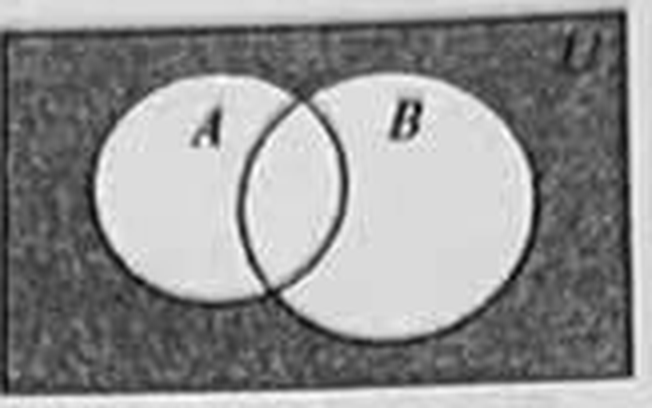
\includegraphics[width=0.30\textwidth]{figures/venn_AB_complement.png}
\end{center}

\ans{$\overline{A\cup B}$}

\ifanswer
\solbegin
\step{图中阴影部分在集合 $A$、$B$ 的外部，即在全集 $U$ 中但不属于 $A$、也不属于 $B$.}
\step{这正是 $A\cup B$ 在全集 $U$ 中的补集，故可表示为 $\overline{A\cup B}$（即 $\complement_U(A\cup B)$）.}
\solend

\fi

\item 设全集 $U=\R$，集合 $A=\{x\mid 2\leqslant x<5\}$，$B=\{x\mid 3<x<6\}$，则 $\overline{A}\cap B=$ \blankline[4.4em]（用区间表示）.

\ans{$[5,6)$}

\ifanswer
\solbegin
\step{在全集 $\R$ 中，$\overline{A}=(-\infty,2)\cup[5,+\infty)$.}
\step{又 $B=(3,6)$，取两集合的公共部分得 $\overline{A}\cap B=[5,6)$.}
\solend

\fi

\item 用反证法证明“$a,b\in\N$，$ab$ 可被 5 整除，那么 $a,b$ 中至少有一个能被 5 整除”时应假设 \blankline[4.4em].

\ans{$a,b$ 都不能被 5 整除}

\ifanswer
\solbegin
\step{反证法需假设结论的反面成立.}
\step{“$a,b$ 中至少有一个能被 5 整除”的反面是“$a,b$ 中没有一个能被 5 整除”，即 $a,b$ 都不能被 5 整除.}
\solend

\fi

\item 满足 $M\subseteq\{a_1,a_2,a_3,a_4,a_5\}$，且 $M\cap\{a_1,a_2,a_3\}=\{a_1,a_2\}$，则集合 $M$ 的个数是 \blankline[2.4em].

\ans{$4$}

\ifanswer
\solbegin
\step{由 $M\cap\{a_1,a_2,a_3\}=\{a_1,a_2\}$ 得 $a_1\in M$，$a_2\in M$，$a_3\notin M$.}
\step{又 $M\subseteq\{a_1,a_2,a_3,a_4,a_5\}$，所以 $a_4$、$a_5$ 可以属于 $M$，也可以不属于 $M$.}
\step{即 $M=\{a_1,a_2\}\cup S$，其中 $S\subseteq\{a_4,a_5\}$，共有 $2^2=4$ 个.}
\solend

\fi

\item 已知集合 $A=\{(x,y)\mid y=x^2\}$，$B=\left\{(x,y)\mid \dfrac{y-1}{x-1}=\dfrac{1}{2}\right\}$，则 $A\cap B=$ \blankline[5.2em].

\ans{$\left\{\left(-\dfrac{1}{2},\dfrac{1}{4}\right)\right\}$}

\ifanswer
\solbegin
\step{集合 $B$ 中的点满足 $y=\dfrac{1}{2}x+\dfrac{1}{2}$，且 $x\neq 1$.}
\step{代入 $y=x^2$ 得 $2x^2-x-1=0$，解得 $x=1$ 或 $x=-\dfrac{1}{2}$.}
\step{因为 $x\neq 1$，所以 $x=-\dfrac{1}{2}$，此时 $y=\dfrac{1}{4}$.}
\step{所以 $A\cap B=\left\{\left(-\dfrac{1}{2},\dfrac{1}{4}\right)\right\}$.}
\solend

\fi

\item 已知集合 $\{a,b,c\}=\{0,1,2\}$，且下列三个关系：①$a\neq 2$ ②$b=2$ ③$c\neq 0$ 有且只有一个正确，则 $100a+10b+c$ 等于 \blankline[2.4em].

\ans{$201$}

\ifanswer
\solbegin
\step{$a,b,c$ 是 $0,1,2$ 的一个排列，共 6 种情形，逐一检验三个关系的真假：}
\step{$(a,b,c)=(0,1,2)$：①真、②假、③真，两个正确，不合；$(0,2,1)$：三个都真，不合；}
\step{$(1,0,2)$：①真、②假、③真，两个正确，不合；$(1,2,0)$：①真、②真、③假，两个正确，不合；}
\step{$(2,0,1)$：①假、②假、③真，恰有一个正确，符合；$(2,1,0)$：三个都假，不合.}
\step{所以 $(a,b,c)=(2,0,1)$，$100a+10b+c=200+0+1=201$.}
\solend

\fi

\item “$x_1>3$ 且 $x_2>3$”是“$x_1+x_2>6$ 且 $x_1x_2>9$”的 \blankline[4.4em] 条件.（选填“充分非必要”，“必要非充分”，“充要”，“既非充分也非必要”）

\ans{充分非必要}

\ifanswer
\solbegin
\step{充分性：若 $x_1>3$ 且 $x_2>3$，则 $x_1+x_2>6$，且 $x_1x_2>9$，故充分性成立.}
\step{必要性：取 $x_1=2$、$x_2=5$，有 $x_1+x_2=7>6$、$x_1x_2=10>9$，但 $x_1>3$ 不成立，故必要性不成立.}
\step{所以应填“充分非必要”.}
\solend

\fi

% 注：第 11 题系 2010 年上海高考理科第 14 题的改写（原题要求选出 4 个子集，官方答案 36）。
%     原题官方解答明言「A、B 可以互换，即视为一种选法」，即**不计先后**计数；
%     按此口径本改写题的答案为 5。（原卷学生作答为 10，是把 A⊆B 与 B⊆A 重复计入。）
\item 在集合 $U=\{a,b,c,d\}$ 的子集中选出 2 个不同的子集，需同时满足以下两个条件：(1)$a,b$ 都要选出 (2)对选出的任意两个子集 $A$ 和 $B$，必有 $A\subseteq B$ 或 $B\subseteq A$，那么共有 \blankline[2.4em] 种不同的选法.

\ans{$5$}

\ifanswer
\solbegin
\step{由 (1) 知 $a,b$ 都要选出，即 $a,b$ 都属于所选的两个子集；由 (2) 知所选的两个子集必须可比.}
\step{含 $a,b$ 的子集只有 $\{a,b\}$、$\{a,b,c\}$、$\{a,b,d\}$、$\{a,b,c,d\}$ 共 4 个.}
\step{在这 4 个子集中取出两个不同的且可比的（一个包含另一个），只有下列 5 组：}
\step{$\{a,b\}\subset\{a,b,c\}$、$\{a,b\}\subset\{a,b,d\}$、$\{a,b\}\subset\{a,b,c,d\}$、$\{a,b,c\}\subset\{a,b,c,d\}$、$\{a,b,d\}\subset\{a,b,c,d\}$.}
\step{注意「选出 2 个子集」的选法\textbf{不计先后}：把这两个子集分别叫作 $A$、$B$ 只是给它们取个名字，$A\subseteq B$ 与 $B\subseteq A$ 说的是同一组子集，算同一种选法.}
\step{（本题由 2010 年上海高考理科第 14 题改写，原题要求选出 4 个子集，其官方答案 36 正是按「$A$、$B$ 可以互换，即视为一种选法」的不计先后口径计数.）}
\step{所以共有 5 种不同的选法.}
\solend

\fi

\end{enumerate}

\bigsec{二、选择题}

\begin{enumerate}
\setcounter{enumi}{11}

\item 已知 $M=(-\infty,\sqrt{3}]$，$a=\sqrt{3}$，则下列关系中正确的是（\quad）.

A. $a\subset M$\qquad B. $a\in M$\qquad C. $\{a\}\in M$\qquad D. $M\subset\{a\}$

\ans{B}

\ifanswer
\solbegin
\step{因为 $\sqrt{3}\leqslant\sqrt{3}$，所以 $a=\sqrt{3}\in M$，B 正确.}
\step{$a$ 是元素、$M$ 是集合，元素与集合之间用 $\in$ 表示，不能用 $\subset$，故 A、D 错误；}
\step{$\{a\}$ 是集合，集合与集合之间应是包含关系（且 $\{a\}\subseteq M$），不能用 $\in$，故 C 错误.}
\step{故选 B.}
\solend

\fi

% 注：原卷此处印作“已知集合{(x,y)|x^2+y^2≤3, x∈Z, y∈Z}”，集合未记作 A，
%     却设问“则 A 中的元素个数是”，显系漏排“A=”；本稿补上，其余照原卷。
\item 已知集合 $A=\{(x,y)\mid x^2+y^2\leqslant 3,\ x\in\Z,\ y\in\Z\}$，则 $A$ 中的元素个数是（\quad）.

A. $9$\qquad B. $8$\qquad C. $5$\qquad D. $4$

\ans{A}

\ifanswer
\solbegin
\step{逐一列举：$x=0$ 时 $y^2\leqslant 3$，$y=-1,0,1$，得 $(0,-1),(0,0),(0,1)$，共 3 个；}
\step{$x=\pm 1$ 时 $y^2\leqslant 2$，$y=-1,0,1$，各得 3 个，共 6 个（$x^2+y^2=2\leqslant 3$ 满足条件）；}
\step{$|x|\geqslant 2$ 时 $x^2\geqslant 4>3$，无解.}
\step{所以 $A$ 中元素个数为 $3+6=9$. 故选 A.}
\solend

\fi

\item 集合 $A=\{x\mid x=(2k-1)\pi,\ k\in\Z\}$ 与 $B=\{x\mid x=(4n\pm 1)\pi,\ n\in\Z\}$ 之间的关系是（\quad）.

A. $A\subset B$\qquad B. $B\subset A$\qquad C. $A=B$\qquad D. 不确定

\ans{C}

\ifanswer
\solbegin
\step{$A$ 由 $\pi$ 的一切奇数倍组成，即 $A=\{\cdots,-3\pi,-\pi,\pi,3\pi,\cdots\}$.}
\step{$B$ 中 $4n+1$ 与 $4n-1$ （$n\in\Z$）都是奇数，故 $B\subseteq A$；}
\step{反之，任一奇数除以 4 的余数只能是 1 或 3：形如 $4m+1$ 的奇数含于 $B$（取 $n=m$），形如 $4m+3=4(m+1)-1$ 的奇数也含于 $B$（取 $n=m+1$），所以 $A\subseteq B$.}
\step{于是 $A\subseteq B$ 且 $B\subseteq A$，即 $A=B$. 故选 C.}
\solend

\fi

\item 设 $T$ 是由正三角形 $P_1P_2P_3$ 边上及其内部的点构成的集合，点 $O$ 是 $\triangle P_1P_2P_3$ 的中心. 若集合 $S=\{P\mid P\in T,\ |PO|\leqslant|PO_i|,\ i=1,2,3\}$，（符号 $|AB|$ 表示平面上两点 $A,B$ 间的距离），则集合 $S$ 表示的平面区域是（\quad）.

A. 四边形区域；\qquad B. 三角形区域；\qquad C. 六边形区域；\qquad D. 五边形区域；

\ans{C}

\ifanswer
\solbegin
\step{$|PO|\leqslant|PO_i|$ 表示点 $P$ 到 $O$ 的距离不大于到顶点 $P_i$ 的距离，即 $P$ 落在线段 $OP_i$ 的垂直平分线靠 $O$ 的那一侧（含该线）.}
\step{对 $i=1,2,3$ 各有一条这样的直线，它们分别把三角形靠近 $P_1$、$P_2$、$P_3$ 的一个小角（三角形）截掉；}
\step{逐一直观验证可知这三条直线两两的交点都在三角形内部，三个角互不重叠，截去三个角后剩下的区域共有 6 条边.}
\step{所以集合 $S$ 表示的平面区域是六边形区域. 故选 C.}
\solend

\fi

\end{enumerate}

\bigsec{三、解答题}

\begin{enumerate}
\setcounter{enumi}{15}

\item（10 分，第 1 小问 5 分，第 2 小问 5 分）已知集合 $A=\{x\mid a\leqslant x\leqslant a+2\}$，集合 $B=\{x\mid x<-1\text{ 或 }x>5\}$，全集 $U=\R$.

\begin{enumerate}[label=(\arabic*)]
\item 若 $a=1$，求 $\overline{A}\cup B$；
\item 若 $A\subseteq B$，求实数 $a$ 的取值范围.
\end{enumerate}

\ans{（1）$(-\infty,1)\cup(3,+\infty)$；（2）$(-\infty,-3)\cup(5,+\infty)$}

\ifanswer
\solbegin
\stepm{(1)}{$a=1$ 时 $A=\{x\mid 1\leqslant x\leqslant 3\}=[1,3]$，则 $\overline{A}=(-\infty,1)\cup(3,+\infty)$.}
\step{又 $B=(-\infty,-1)\cup(5,+\infty)$，而 $B\subseteq\overline{A}$（因 $5>3$、$-1<1$），}
\step{所以 $\overline{A}\cup B=(-\infty,1)\cup(3,+\infty)$.}
\stepm{(2)}{因为 $a\leqslant a+2$，所以集合 $A=\{x\mid a\leqslant x\leqslant a+2\}$ 始终非空.}
\step{要使 $A\subseteq B$，只需 $A$ 与 $[-1,5]$ 没有公共点，即 $a+2<-1$ 或 $a>5$.}
\step{解得 $a<-3$ 或 $a>5$，所以实数 $a$ 的取值范围是 $(-\infty,-3)\cup(5,+\infty)$.}
\solend

\fi

\ansspace[10]

\item（10 分，第 1 小问 5 分，第 2 小问 5 分）已知 $A=\{x\mid x^2+x-2=0\}$，$B=\{x\mid x^2+ax+2a-4=0\}$.

\begin{enumerate}[label=(\arabic*)]
\item 若 $A=B$，求实数 $a$ 的值；
\item 若 $B\subseteq A$，求实数 $a$ 的值.
\end{enumerate}

\ans{（1）$a=1$；（2）$a=1$ 或 $a=4$}

\ifanswer
\solbegin
\stepm{(1)}{由 $x^2+x-2=0$ 解得 $x=1$ 或 $x=-2$，所以 $A=\{1,-2\}$.}
\step{由 $A=B$ 知 $1$、$-2$ 是方程 $x^2+ax+2a-4=0$ 的两根，由根与系数的关系得 $1+(-2)=-a$，所以 $a=1$；}
\step{此时 $2a-4=-2=1\times(-2)$，与两根之积相符，故 $a=1$.}
\stepm{(2)}{方程 $x^2+ax+2a-4=0$ 的判别式 $\Delta=a^2-4(2a-4)=(a-4)^2\geqslant 0$ 恒成立，所以集合 $B$ 不可能是空集.}
\step{由 $B\subseteq A$ 知 $B=\{1\}$ 或 $B=\{-2\}$ 或 $B=\{1,-2\}$.}
\step{若 $B=\{1\}$，则 $1$ 是二重根，$1+1=-a$ 且 $1\times 1=2a-4$，即 $a=-2$ 且 $a=\dfrac{5}{2}$，无解；}
\step{若 $B=\{-2\}$，则 $-2$ 是二重根，$(-2)+(-2)=-a$ 且 $(-2)\times(-2)=2a-4$，两式都给出 $a=4$，符合；}
\step{若 $B=\{1,-2\}$，则 $1+(-2)=-a$，得 $a=1$，此时 $2a-4=-2=1\times(-2)$，符合.}
\step{综上，$a=1$ 或 $a=4$.}
\solend

\fi

\ansspace[12]

\item（11 分，第 1 小问 3 分，第 2 小问 3 分，第 3 小问 5 分）已知非空数集 $S$ 满足：对任意给定的 $x,y\in S$（$x,y$ 可以相同），有 $x+y\in S$ 且 $x-y\in S$.

\begin{enumerate}[label=(\arabic*)]
\item 哪个数一定是 $S$ 中的元素?说明理由；
\item 若 $S$ 是有限集，求 $S$；
\item 若 $S$ 中最小的正数为 5，求 $S$.
\end{enumerate}

\ans{（1）$0$；（2）$S=\{0\}$；（3）$S=\{x\mid x=5a,\ a\in\Z\}$}

\ifanswer
\solbegin
\stepm{(1)}{$0$ 一定是 $S$ 中的元素. 理由：$S$ 非空，取 $x\in S$，在 $x-y\in S$ 中令 $y=x$（$x,y$ 可以相同），得 $x-x=0\in S$.}
\stepm{(2)}{若 $S$ 是有限集，则 $S=\{0\}$. 理由：取 $x\in S$ 且 $x\neq 0$，由 $x+y\in S$ 依次得 $2x=x+x\in S$，$3x=2x+x\in S$，$\cdots$，即 $kx\in S$（$k=1,2,3,\cdots$）；}
\step{这些数互不相同，与 $S$ 是有限集矛盾，所以 $S$ 中除 $0$ 外没有别的元素，即 $S=\{0\}$（此时 $0+0=0\in S$，$0-0=0\in S$，符合条件）.}
\stepm{(3)}{因为 $5\in S$，由 $x+y\in S$ 得 $5+5=10\in S$，$10+5=15\in S$，$\cdots$，故一切正整数倍的 $5$ 都在 $S$ 中；}
\step{又由 $x-y\in S$ 得 $5-5=0\in S$，$0-5=-5\in S$，$-5-5=-10\in S$，$\cdots$，故一切负整数倍的 $5$ 也都在 $S$ 中，即 $\{5a\mid a\in\Z\}\subseteq S$.}
\step{反之，任取 $s\in S$，由 $5\in S$ 及封闭性知 $s-5k\in S$（$k\in\Z$）；把 $s$ 写成 $s=5q+r$（$q\in\Z$，$0\leqslant r<5$），取 $k=q$ 得 $r=s-5q\in S$.}
\step{若 $r>0$，则 $S$ 中有比 $5$ 更小的正数 $r$，与“$S$ 中最小的正数为 5”矛盾，故只能 $r=0$，即 $s=5q$.}
\step{所以 $S=\{x\mid x=5a,\ a\in\Z\}$.}
\solend

\fi

\ansspace[12]

\end{enumerate}

\bigsec{附加题}

\begin{enumerate}
\setcounter{enumi}{18}

\item 已知集合 $A,B,C\subseteq\{1,2,3,\cdots,2024\}$，且 $A\subseteq B\subseteq C$，则有序集合组 $(A,B,C)$ 的个数是 \blankline[3.2em].

\ans{$4^{2024}$}

\ifanswer
\solbegin
\step{对 $U=\{1,2,\cdots,2024\}$ 中的每个元素，它与 $A,B,C$ 的关系只有四种可能：}
\step{在 $A,B,C$ 中都出现；不在 $A$ 中而在 $B,C$ 中出现；只在 $C$ 中出现；在三个集合中都不出现.}
\step{反过来，任取每个元素的一种归属方式，都恰好得到一个满足 $A\subseteq B\subseteq C$ 的有序集合组，故不同的组与不同的归属方式一一对应.}
\step{所以共有 $4\times 4\times\cdots\times 4=4^{2024}$ 个有序集合组.}
\solend

\fi

\item 已知集合 $M=\{1,2,\cdots,10\}$，对它的非空子集 $A$，将 $A$ 中的每个元素 $k$ 都乘以 $(-1)^k$ 再求和，如 $A=\{2,3,6\}$，可求得和为 $(-1)^2\times 2+(-1)^3\times 3+(-1)^6\times 6=5$. 试对 $M$ 的所有非空子集，求这些和的总和 \blankline[3.2em].

\ans{$2560$}

\ifanswer
\solbegin
\step{元素 $k$（$k=1,2,\cdots,10$）出现在 $M$ 的 $2^{9}$ 个非空子集中（其余 9 个元素任取）.}
\step{所以在所有非空子集的和中，$k$ 贡献的总量为 $2^{9}\times(-1)^k\cdot k=512\times(-1)^kk$.}
\step{于是这些和的总和为 $512\displaystyle\sum_{k=1}^{10}(-1)^kk=512\times(-1+2-3+4-5+6-7+8-9+10)=512\times 5=2560$.}
\solend

\fi

\item 设 $a_1,a_2,a_3,a_4$ 是 4 个有理数，使得 $\{a_ia_j\mid 1\leqslant i<j\leqslant 4\}=\left\{-24,-2,-\dfrac{3}{2},-\dfrac{1}{8},1,3\right\}$. 求 $a_1+a_2+a_3+a_4=$ \blankline[3.2em].

\ans{$\pm\dfrac{9}{4}$（两组解，和分别为 $-\dfrac{9}{4}$ 与 $\dfrac{9}{4}$）}

\ifanswer
\solbegin
\step{六个乘积中有 4 个负数、2 个正数. 设 4 个数中正数有 $p$ 个、负数有 $q$ 个（$p+q=4$），则异号的两数相乘得负数，其个数为 $pq$；由 $pq=4$ 得 $p=q=2$，即恰有 2 个正数、2 个负数.}
\step{把 4 个数的绝对值记作 $w,x,y,z>0$，则六个两两乘积的绝对值为 $24,2,\dfrac{3}{2},\dfrac{1}{8},1,3$；其中 $1$ 与 $3$ 来自两对同号的数，$24,2,\dfrac{3}{2},\dfrac{1}{8}$ 来自四对异号的数.}
\step{由 $(a_1a_2a_3a_4)^3=(-24)\times(-2)\times\left(-\dfrac{3}{2}\right)\times\left(-\dfrac{1}{8}\right)\times 1\times 3=27$ 得 $a_1a_2a_3a_4=3$，即去符号后 $wxyz=3$.}
\step{逐一检验可知 $w,x,y,z$ 只能是 $\left\{4,\dfrac{1}{4},6,\dfrac{1}{2}\right\}$：其中 $4\times\dfrac{1}{4}=1$、$6\times\dfrac{1}{2}=3$ 为同号两对的乘积，$4\times 6=24$、$4\times\dfrac{1}{2}=2$、$\dfrac{1}{4}\times 6=\dfrac{3}{2}$、$\dfrac{1}{4}\times\dfrac{1}{2}=\dfrac{1}{8}$ 为异号四对的乘积.}
\step{于是 $\left\{4,\dfrac{1}{4}\right\}$ 中的两个数同号、$\left\{6,\dfrac{1}{2}\right\}$ 中的两个数同号，且这两组异号，得两组解：}
\step{$4,\ \dfrac{1}{4},\ -6,\ -\dfrac{1}{2}$，和为 $-\dfrac{9}{4}$；\quad 或 \quad $6,\ \dfrac{1}{2},\ -4,\ -\dfrac{1}{4}$，和为 $\dfrac{9}{4}$.}
\step{两组解的六个乘积都恰为 $-24,-2,-\dfrac{3}{2},-\dfrac{1}{8},1,3$，与原卷所给集合相同.}
\step{所以 $a_1+a_2+a_3+a_4=\pm\dfrac{9}{4}$.}
\solend

\fi

\end{enumerate}

\end{document}
"
% 紧凑版：xelatex "\def\iscompact{1}% 高一16_大同中学_第二周周末练习1.tex —— 高一上数学「第二周周末练习1」（试卷版/答案版）
% 试卷版：xelatex 高一16_大同中学_第二周周末练习1.tex
% 答案版：xelatex "\def\isanswer{1}\input{高一16_大同中学_第二周周末练习1.tex}"
% 紧凑版：xelatex "\def\iscompact{1}\input{高一16_大同中学_第二周周末练习1.tex}"
%
% 原始材料为学生作业的手机翻拍照片（卷面为学生本人的**手写作答**，未见教师批改痕迹）。
% 试题文字照原卷录入；答案版给出的是**经核验的正确解答与解析**，与原卷手写答案的差异见 README。
%
% 与原卷的两处排版差异（均已在 README「说明」中交代）：
%   ① 原卷未印分节标题与分值，本稿按题型补「一、填空题 / 二、选择题 / 三、解答题」三节
%      （「附加题」原卷有印）；
%   ② 第 13 题原卷印作「已知集合{(x,y)|…}」，集合未记作 A 却被设问为「A 中的元素个数」，
%      显系漏排「A=」，本稿补上。

% 本篇的正文与家长拍照卷 `高一b_大同中学_第二周周末练习1（补）` **完全相同**——同一份作业，
% 试卷版/答案版也都是同一份源码编译而来；`高一b` 的 4 张原图另存于
% `原图/高一b_大同中学_第二周周末练习1（补）/`，本卷 `原图/` 下是同一组照片的副本。
% 经核对，这份作业就是公众号「魔都数学加油站」连载「27学年高一16——2026-2027年上海市大同中学
% 高一上周末作业2.1」的那一份：**题号与题干逐题一致**，只是公众号版略去了填空第 1、2 题，
% 故拍照卷反而是更完整的版本（对照关系见 README「与公众号连载号的对照表」）。
%
% 本卷的编号与连载号对齐（高一16），卷面标题因此**不带**「（补）」；标题里的「大同中学」为**本稿所加**
% （原卷标题只有作业名，校名只印在页眉「上海市大同…」）。带「（补）」的 `高一b` 保留为
% 拍照原件的转录本，两者内容一字不差。
%
% 一处与公众号讲评版的差异需留意：本卷第 11 题的答案按 2010 年上海高考理科第 14 题官方解答
% 「A、B 可以互换，即视为一种选法」的不计先后口径取 5，而公众号讲评版把它按有先后的 32 计数
% （该题学生原作答为 10）。取舍理由见该题下的 `%` 注。
\documentclass[a4paper,11pt]{article}
\usepackage{common}

\begin{document}

\examtitlest[3]{2026--2027 学年度大同中学高一上数学第二周周末练习1}{集合与常用逻辑用语}

\bigsec{一、填空题}

\begin{enumerate}

\item 用列举法表示集合 $\{x\mid -2<x\leqslant 2,\ x\in\Z\}=$ \blankline[2.4em].

\ans{$\{-1,0,1,2\}$}

\ifanswer
\solbegin
\step{集合中的元素是满足 $-2<x\leqslant 2$ 的整数，即 $-1$、$0$、$1$、$2$.}
\step{所以用列举法表示为 $\{-1,0,1,2\}$.}
\solend

\fi

\item 设集合 $A=\{1,a\}$，$B=\{1,a^2\}$，若 $A=B$，则实数 $a$ 的值为 \blankline[2.4em].

\ans{$a=0$}

\ifanswer
\solbegin
\step{由 $A=B$ 得 $a^2=a$，解得 $a=0$ 或 $a=1$.}
\step{当 $a=1$ 时，$A=\{1,1\}$，不符合集合元素的互异性，舍去；}
\step{当 $a=0$ 时，$A=\{1,0\}$，$B=\{1,0\}$，两集合相等，符合条件.}
\step{所以 $a=0$.}
\solend

\fi

\item 已知集合 $A=\{0,2,3,4,5\}$，$B=\{2,3,5,7\}$，$C=\{2,3,6\}$，则 $(A\cap B)\cup C=$ \blankline[4.4em].

\ans{$\{2,3,5,6\}$}

\ifanswer
\solbegin
\step{$A\cap B=\{0,2,3,4,5\}\cap\{2,3,5,7\}=\{2,3,5\}$.}
\step{所以 $(A\cap B)\cup C=\{2,3,5\}\cup\{2,3,6\}=\{2,3,5,6\}$.}
\solend

\fi

\item 设全集为 $U$，用集合 $A,B$ 的交、并或补集符号表示图中的阴影部分是 \blankline[4.4em].

\begin{center}
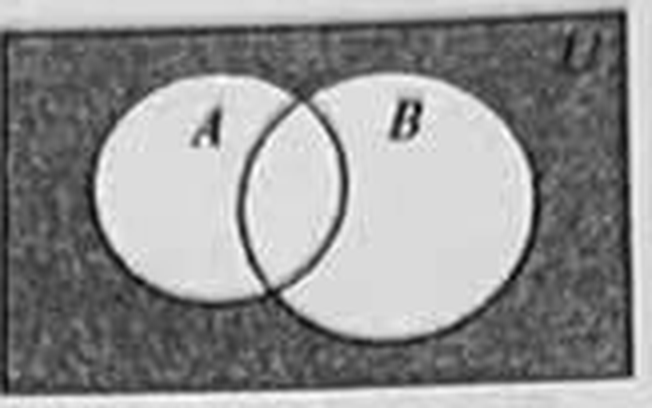
\includegraphics[width=0.30\textwidth]{figures/venn_AB_complement.png}
\end{center}

\ans{$\overline{A\cup B}$}

\ifanswer
\solbegin
\step{图中阴影部分在集合 $A$、$B$ 的外部，即在全集 $U$ 中但不属于 $A$、也不属于 $B$.}
\step{这正是 $A\cup B$ 在全集 $U$ 中的补集，故可表示为 $\overline{A\cup B}$（即 $\complement_U(A\cup B)$）.}
\solend

\fi

\item 设全集 $U=\R$，集合 $A=\{x\mid 2\leqslant x<5\}$，$B=\{x\mid 3<x<6\}$，则 $\overline{A}\cap B=$ \blankline[4.4em]（用区间表示）.

\ans{$[5,6)$}

\ifanswer
\solbegin
\step{在全集 $\R$ 中，$\overline{A}=(-\infty,2)\cup[5,+\infty)$.}
\step{又 $B=(3,6)$，取两集合的公共部分得 $\overline{A}\cap B=[5,6)$.}
\solend

\fi

\item 用反证法证明“$a,b\in\N$，$ab$ 可被 5 整除，那么 $a,b$ 中至少有一个能被 5 整除”时应假设 \blankline[4.4em].

\ans{$a,b$ 都不能被 5 整除}

\ifanswer
\solbegin
\step{反证法需假设结论的反面成立.}
\step{“$a,b$ 中至少有一个能被 5 整除”的反面是“$a,b$ 中没有一个能被 5 整除”，即 $a,b$ 都不能被 5 整除.}
\solend

\fi

\item 满足 $M\subseteq\{a_1,a_2,a_3,a_4,a_5\}$，且 $M\cap\{a_1,a_2,a_3\}=\{a_1,a_2\}$，则集合 $M$ 的个数是 \blankline[2.4em].

\ans{$4$}

\ifanswer
\solbegin
\step{由 $M\cap\{a_1,a_2,a_3\}=\{a_1,a_2\}$ 得 $a_1\in M$，$a_2\in M$，$a_3\notin M$.}
\step{又 $M\subseteq\{a_1,a_2,a_3,a_4,a_5\}$，所以 $a_4$、$a_5$ 可以属于 $M$，也可以不属于 $M$.}
\step{即 $M=\{a_1,a_2\}\cup S$，其中 $S\subseteq\{a_4,a_5\}$，共有 $2^2=4$ 个.}
\solend

\fi

\item 已知集合 $A=\{(x,y)\mid y=x^2\}$，$B=\left\{(x,y)\mid \dfrac{y-1}{x-1}=\dfrac{1}{2}\right\}$，则 $A\cap B=$ \blankline[5.2em].

\ans{$\left\{\left(-\dfrac{1}{2},\dfrac{1}{4}\right)\right\}$}

\ifanswer
\solbegin
\step{集合 $B$ 中的点满足 $y=\dfrac{1}{2}x+\dfrac{1}{2}$，且 $x\neq 1$.}
\step{代入 $y=x^2$ 得 $2x^2-x-1=0$，解得 $x=1$ 或 $x=-\dfrac{1}{2}$.}
\step{因为 $x\neq 1$，所以 $x=-\dfrac{1}{2}$，此时 $y=\dfrac{1}{4}$.}
\step{所以 $A\cap B=\left\{\left(-\dfrac{1}{2},\dfrac{1}{4}\right)\right\}$.}
\solend

\fi

\item 已知集合 $\{a,b,c\}=\{0,1,2\}$，且下列三个关系：①$a\neq 2$ ②$b=2$ ③$c\neq 0$ 有且只有一个正确，则 $100a+10b+c$ 等于 \blankline[2.4em].

\ans{$201$}

\ifanswer
\solbegin
\step{$a,b,c$ 是 $0,1,2$ 的一个排列，共 6 种情形，逐一检验三个关系的真假：}
\step{$(a,b,c)=(0,1,2)$：①真、②假、③真，两个正确，不合；$(0,2,1)$：三个都真，不合；}
\step{$(1,0,2)$：①真、②假、③真，两个正确，不合；$(1,2,0)$：①真、②真、③假，两个正确，不合；}
\step{$(2,0,1)$：①假、②假、③真，恰有一个正确，符合；$(2,1,0)$：三个都假，不合.}
\step{所以 $(a,b,c)=(2,0,1)$，$100a+10b+c=200+0+1=201$.}
\solend

\fi

\item “$x_1>3$ 且 $x_2>3$”是“$x_1+x_2>6$ 且 $x_1x_2>9$”的 \blankline[4.4em] 条件.（选填“充分非必要”，“必要非充分”，“充要”，“既非充分也非必要”）

\ans{充分非必要}

\ifanswer
\solbegin
\step{充分性：若 $x_1>3$ 且 $x_2>3$，则 $x_1+x_2>6$，且 $x_1x_2>9$，故充分性成立.}
\step{必要性：取 $x_1=2$、$x_2=5$，有 $x_1+x_2=7>6$、$x_1x_2=10>9$，但 $x_1>3$ 不成立，故必要性不成立.}
\step{所以应填“充分非必要”.}
\solend

\fi

% 注：第 11 题系 2010 年上海高考理科第 14 题的改写（原题要求选出 4 个子集，官方答案 36）。
%     原题官方解答明言「A、B 可以互换，即视为一种选法」，即**不计先后**计数；
%     按此口径本改写题的答案为 5。（原卷学生作答为 10，是把 A⊆B 与 B⊆A 重复计入。）
\item 在集合 $U=\{a,b,c,d\}$ 的子集中选出 2 个不同的子集，需同时满足以下两个条件：(1)$a,b$ 都要选出 (2)对选出的任意两个子集 $A$ 和 $B$，必有 $A\subseteq B$ 或 $B\subseteq A$，那么共有 \blankline[2.4em] 种不同的选法.

\ans{$5$}

\ifanswer
\solbegin
\step{由 (1) 知 $a,b$ 都要选出，即 $a,b$ 都属于所选的两个子集；由 (2) 知所选的两个子集必须可比.}
\step{含 $a,b$ 的子集只有 $\{a,b\}$、$\{a,b,c\}$、$\{a,b,d\}$、$\{a,b,c,d\}$ 共 4 个.}
\step{在这 4 个子集中取出两个不同的且可比的（一个包含另一个），只有下列 5 组：}
\step{$\{a,b\}\subset\{a,b,c\}$、$\{a,b\}\subset\{a,b,d\}$、$\{a,b\}\subset\{a,b,c,d\}$、$\{a,b,c\}\subset\{a,b,c,d\}$、$\{a,b,d\}\subset\{a,b,c,d\}$.}
\step{注意「选出 2 个子集」的选法\textbf{不计先后}：把这两个子集分别叫作 $A$、$B$ 只是给它们取个名字，$A\subseteq B$ 与 $B\subseteq A$ 说的是同一组子集，算同一种选法.}
\step{（本题由 2010 年上海高考理科第 14 题改写，原题要求选出 4 个子集，其官方答案 36 正是按「$A$、$B$ 可以互换，即视为一种选法」的不计先后口径计数.）}
\step{所以共有 5 种不同的选法.}
\solend

\fi

\end{enumerate}

\bigsec{二、选择题}

\begin{enumerate}
\setcounter{enumi}{11}

\item 已知 $M=(-\infty,\sqrt{3}]$，$a=\sqrt{3}$，则下列关系中正确的是（\quad）.

A. $a\subset M$\qquad B. $a\in M$\qquad C. $\{a\}\in M$\qquad D. $M\subset\{a\}$

\ans{B}

\ifanswer
\solbegin
\step{因为 $\sqrt{3}\leqslant\sqrt{3}$，所以 $a=\sqrt{3}\in M$，B 正确.}
\step{$a$ 是元素、$M$ 是集合，元素与集合之间用 $\in$ 表示，不能用 $\subset$，故 A、D 错误；}
\step{$\{a\}$ 是集合，集合与集合之间应是包含关系（且 $\{a\}\subseteq M$），不能用 $\in$，故 C 错误.}
\step{故选 B.}
\solend

\fi

% 注：原卷此处印作“已知集合{(x,y)|x^2+y^2≤3, x∈Z, y∈Z}”，集合未记作 A，
%     却设问“则 A 中的元素个数是”，显系漏排“A=”；本稿补上，其余照原卷。
\item 已知集合 $A=\{(x,y)\mid x^2+y^2\leqslant 3,\ x\in\Z,\ y\in\Z\}$，则 $A$ 中的元素个数是（\quad）.

A. $9$\qquad B. $8$\qquad C. $5$\qquad D. $4$

\ans{A}

\ifanswer
\solbegin
\step{逐一列举：$x=0$ 时 $y^2\leqslant 3$，$y=-1,0,1$，得 $(0,-1),(0,0),(0,1)$，共 3 个；}
\step{$x=\pm 1$ 时 $y^2\leqslant 2$，$y=-1,0,1$，各得 3 个，共 6 个（$x^2+y^2=2\leqslant 3$ 满足条件）；}
\step{$|x|\geqslant 2$ 时 $x^2\geqslant 4>3$，无解.}
\step{所以 $A$ 中元素个数为 $3+6=9$. 故选 A.}
\solend

\fi

\item 集合 $A=\{x\mid x=(2k-1)\pi,\ k\in\Z\}$ 与 $B=\{x\mid x=(4n\pm 1)\pi,\ n\in\Z\}$ 之间的关系是（\quad）.

A. $A\subset B$\qquad B. $B\subset A$\qquad C. $A=B$\qquad D. 不确定

\ans{C}

\ifanswer
\solbegin
\step{$A$ 由 $\pi$ 的一切奇数倍组成，即 $A=\{\cdots,-3\pi,-\pi,\pi,3\pi,\cdots\}$.}
\step{$B$ 中 $4n+1$ 与 $4n-1$ （$n\in\Z$）都是奇数，故 $B\subseteq A$；}
\step{反之，任一奇数除以 4 的余数只能是 1 或 3：形如 $4m+1$ 的奇数含于 $B$（取 $n=m$），形如 $4m+3=4(m+1)-1$ 的奇数也含于 $B$（取 $n=m+1$），所以 $A\subseteq B$.}
\step{于是 $A\subseteq B$ 且 $B\subseteq A$，即 $A=B$. 故选 C.}
\solend

\fi

\item 设 $T$ 是由正三角形 $P_1P_2P_3$ 边上及其内部的点构成的集合，点 $O$ 是 $\triangle P_1P_2P_3$ 的中心. 若集合 $S=\{P\mid P\in T,\ |PO|\leqslant|PO_i|,\ i=1,2,3\}$，（符号 $|AB|$ 表示平面上两点 $A,B$ 间的距离），则集合 $S$ 表示的平面区域是（\quad）.

A. 四边形区域；\qquad B. 三角形区域；\qquad C. 六边形区域；\qquad D. 五边形区域；

\ans{C}

\ifanswer
\solbegin
\step{$|PO|\leqslant|PO_i|$ 表示点 $P$ 到 $O$ 的距离不大于到顶点 $P_i$ 的距离，即 $P$ 落在线段 $OP_i$ 的垂直平分线靠 $O$ 的那一侧（含该线）.}
\step{对 $i=1,2,3$ 各有一条这样的直线，它们分别把三角形靠近 $P_1$、$P_2$、$P_3$ 的一个小角（三角形）截掉；}
\step{逐一直观验证可知这三条直线两两的交点都在三角形内部，三个角互不重叠，截去三个角后剩下的区域共有 6 条边.}
\step{所以集合 $S$ 表示的平面区域是六边形区域. 故选 C.}
\solend

\fi

\end{enumerate}

\bigsec{三、解答题}

\begin{enumerate}
\setcounter{enumi}{15}

\item（10 分，第 1 小问 5 分，第 2 小问 5 分）已知集合 $A=\{x\mid a\leqslant x\leqslant a+2\}$，集合 $B=\{x\mid x<-1\text{ 或 }x>5\}$，全集 $U=\R$.

\begin{enumerate}[label=(\arabic*)]
\item 若 $a=1$，求 $\overline{A}\cup B$；
\item 若 $A\subseteq B$，求实数 $a$ 的取值范围.
\end{enumerate}

\ans{（1）$(-\infty,1)\cup(3,+\infty)$；（2）$(-\infty,-3)\cup(5,+\infty)$}

\ifanswer
\solbegin
\stepm{(1)}{$a=1$ 时 $A=\{x\mid 1\leqslant x\leqslant 3\}=[1,3]$，则 $\overline{A}=(-\infty,1)\cup(3,+\infty)$.}
\step{又 $B=(-\infty,-1)\cup(5,+\infty)$，而 $B\subseteq\overline{A}$（因 $5>3$、$-1<1$），}
\step{所以 $\overline{A}\cup B=(-\infty,1)\cup(3,+\infty)$.}
\stepm{(2)}{因为 $a\leqslant a+2$，所以集合 $A=\{x\mid a\leqslant x\leqslant a+2\}$ 始终非空.}
\step{要使 $A\subseteq B$，只需 $A$ 与 $[-1,5]$ 没有公共点，即 $a+2<-1$ 或 $a>5$.}
\step{解得 $a<-3$ 或 $a>5$，所以实数 $a$ 的取值范围是 $(-\infty,-3)\cup(5,+\infty)$.}
\solend

\fi

\ansspace[10]

\item（10 分，第 1 小问 5 分，第 2 小问 5 分）已知 $A=\{x\mid x^2+x-2=0\}$，$B=\{x\mid x^2+ax+2a-4=0\}$.

\begin{enumerate}[label=(\arabic*)]
\item 若 $A=B$，求实数 $a$ 的值；
\item 若 $B\subseteq A$，求实数 $a$ 的值.
\end{enumerate}

\ans{（1）$a=1$；（2）$a=1$ 或 $a=4$}

\ifanswer
\solbegin
\stepm{(1)}{由 $x^2+x-2=0$ 解得 $x=1$ 或 $x=-2$，所以 $A=\{1,-2\}$.}
\step{由 $A=B$ 知 $1$、$-2$ 是方程 $x^2+ax+2a-4=0$ 的两根，由根与系数的关系得 $1+(-2)=-a$，所以 $a=1$；}
\step{此时 $2a-4=-2=1\times(-2)$，与两根之积相符，故 $a=1$.}
\stepm{(2)}{方程 $x^2+ax+2a-4=0$ 的判别式 $\Delta=a^2-4(2a-4)=(a-4)^2\geqslant 0$ 恒成立，所以集合 $B$ 不可能是空集.}
\step{由 $B\subseteq A$ 知 $B=\{1\}$ 或 $B=\{-2\}$ 或 $B=\{1,-2\}$.}
\step{若 $B=\{1\}$，则 $1$ 是二重根，$1+1=-a$ 且 $1\times 1=2a-4$，即 $a=-2$ 且 $a=\dfrac{5}{2}$，无解；}
\step{若 $B=\{-2\}$，则 $-2$ 是二重根，$(-2)+(-2)=-a$ 且 $(-2)\times(-2)=2a-4$，两式都给出 $a=4$，符合；}
\step{若 $B=\{1,-2\}$，则 $1+(-2)=-a$，得 $a=1$，此时 $2a-4=-2=1\times(-2)$，符合.}
\step{综上，$a=1$ 或 $a=4$.}
\solend

\fi

\ansspace[12]

\item（11 分，第 1 小问 3 分，第 2 小问 3 分，第 3 小问 5 分）已知非空数集 $S$ 满足：对任意给定的 $x,y\in S$（$x,y$ 可以相同），有 $x+y\in S$ 且 $x-y\in S$.

\begin{enumerate}[label=(\arabic*)]
\item 哪个数一定是 $S$ 中的元素?说明理由；
\item 若 $S$ 是有限集，求 $S$；
\item 若 $S$ 中最小的正数为 5，求 $S$.
\end{enumerate}

\ans{（1）$0$；（2）$S=\{0\}$；（3）$S=\{x\mid x=5a,\ a\in\Z\}$}

\ifanswer
\solbegin
\stepm{(1)}{$0$ 一定是 $S$ 中的元素. 理由：$S$ 非空，取 $x\in S$，在 $x-y\in S$ 中令 $y=x$（$x,y$ 可以相同），得 $x-x=0\in S$.}
\stepm{(2)}{若 $S$ 是有限集，则 $S=\{0\}$. 理由：取 $x\in S$ 且 $x\neq 0$，由 $x+y\in S$ 依次得 $2x=x+x\in S$，$3x=2x+x\in S$，$\cdots$，即 $kx\in S$（$k=1,2,3,\cdots$）；}
\step{这些数互不相同，与 $S$ 是有限集矛盾，所以 $S$ 中除 $0$ 外没有别的元素，即 $S=\{0\}$（此时 $0+0=0\in S$，$0-0=0\in S$，符合条件）.}
\stepm{(3)}{因为 $5\in S$，由 $x+y\in S$ 得 $5+5=10\in S$，$10+5=15\in S$，$\cdots$，故一切正整数倍的 $5$ 都在 $S$ 中；}
\step{又由 $x-y\in S$ 得 $5-5=0\in S$，$0-5=-5\in S$，$-5-5=-10\in S$，$\cdots$，故一切负整数倍的 $5$ 也都在 $S$ 中，即 $\{5a\mid a\in\Z\}\subseteq S$.}
\step{反之，任取 $s\in S$，由 $5\in S$ 及封闭性知 $s-5k\in S$（$k\in\Z$）；把 $s$ 写成 $s=5q+r$（$q\in\Z$，$0\leqslant r<5$），取 $k=q$ 得 $r=s-5q\in S$.}
\step{若 $r>0$，则 $S$ 中有比 $5$ 更小的正数 $r$，与“$S$ 中最小的正数为 5”矛盾，故只能 $r=0$，即 $s=5q$.}
\step{所以 $S=\{x\mid x=5a,\ a\in\Z\}$.}
\solend

\fi

\ansspace[12]

\end{enumerate}

\bigsec{附加题}

\begin{enumerate}
\setcounter{enumi}{18}

\item 已知集合 $A,B,C\subseteq\{1,2,3,\cdots,2024\}$，且 $A\subseteq B\subseteq C$，则有序集合组 $(A,B,C)$ 的个数是 \blankline[3.2em].

\ans{$4^{2024}$}

\ifanswer
\solbegin
\step{对 $U=\{1,2,\cdots,2024\}$ 中的每个元素，它与 $A,B,C$ 的关系只有四种可能：}
\step{在 $A,B,C$ 中都出现；不在 $A$ 中而在 $B,C$ 中出现；只在 $C$ 中出现；在三个集合中都不出现.}
\step{反过来，任取每个元素的一种归属方式，都恰好得到一个满足 $A\subseteq B\subseteq C$ 的有序集合组，故不同的组与不同的归属方式一一对应.}
\step{所以共有 $4\times 4\times\cdots\times 4=4^{2024}$ 个有序集合组.}
\solend

\fi

\item 已知集合 $M=\{1,2,\cdots,10\}$，对它的非空子集 $A$，将 $A$ 中的每个元素 $k$ 都乘以 $(-1)^k$ 再求和，如 $A=\{2,3,6\}$，可求得和为 $(-1)^2\times 2+(-1)^3\times 3+(-1)^6\times 6=5$. 试对 $M$ 的所有非空子集，求这些和的总和 \blankline[3.2em].

\ans{$2560$}

\ifanswer
\solbegin
\step{元素 $k$（$k=1,2,\cdots,10$）出现在 $M$ 的 $2^{9}$ 个非空子集中（其余 9 个元素任取）.}
\step{所以在所有非空子集的和中，$k$ 贡献的总量为 $2^{9}\times(-1)^k\cdot k=512\times(-1)^kk$.}
\step{于是这些和的总和为 $512\displaystyle\sum_{k=1}^{10}(-1)^kk=512\times(-1+2-3+4-5+6-7+8-9+10)=512\times 5=2560$.}
\solend

\fi

\item 设 $a_1,a_2,a_3,a_4$ 是 4 个有理数，使得 $\{a_ia_j\mid 1\leqslant i<j\leqslant 4\}=\left\{-24,-2,-\dfrac{3}{2},-\dfrac{1}{8},1,3\right\}$. 求 $a_1+a_2+a_3+a_4=$ \blankline[3.2em].

\ans{$\pm\dfrac{9}{4}$（两组解，和分别为 $-\dfrac{9}{4}$ 与 $\dfrac{9}{4}$）}

\ifanswer
\solbegin
\step{六个乘积中有 4 个负数、2 个正数. 设 4 个数中正数有 $p$ 个、负数有 $q$ 个（$p+q=4$），则异号的两数相乘得负数，其个数为 $pq$；由 $pq=4$ 得 $p=q=2$，即恰有 2 个正数、2 个负数.}
\step{把 4 个数的绝对值记作 $w,x,y,z>0$，则六个两两乘积的绝对值为 $24,2,\dfrac{3}{2},\dfrac{1}{8},1,3$；其中 $1$ 与 $3$ 来自两对同号的数，$24,2,\dfrac{3}{2},\dfrac{1}{8}$ 来自四对异号的数.}
\step{由 $(a_1a_2a_3a_4)^3=(-24)\times(-2)\times\left(-\dfrac{3}{2}\right)\times\left(-\dfrac{1}{8}\right)\times 1\times 3=27$ 得 $a_1a_2a_3a_4=3$，即去符号后 $wxyz=3$.}
\step{逐一检验可知 $w,x,y,z$ 只能是 $\left\{4,\dfrac{1}{4},6,\dfrac{1}{2}\right\}$：其中 $4\times\dfrac{1}{4}=1$、$6\times\dfrac{1}{2}=3$ 为同号两对的乘积，$4\times 6=24$、$4\times\dfrac{1}{2}=2$、$\dfrac{1}{4}\times 6=\dfrac{3}{2}$、$\dfrac{1}{4}\times\dfrac{1}{2}=\dfrac{1}{8}$ 为异号四对的乘积.}
\step{于是 $\left\{4,\dfrac{1}{4}\right\}$ 中的两个数同号、$\left\{6,\dfrac{1}{2}\right\}$ 中的两个数同号，且这两组异号，得两组解：}
\step{$4,\ \dfrac{1}{4},\ -6,\ -\dfrac{1}{2}$，和为 $-\dfrac{9}{4}$；\quad 或 \quad $6,\ \dfrac{1}{2},\ -4,\ -\dfrac{1}{4}$，和为 $\dfrac{9}{4}$.}
\step{两组解的六个乘积都恰为 $-24,-2,-\dfrac{3}{2},-\dfrac{1}{8},1,3$，与原卷所给集合相同.}
\step{所以 $a_1+a_2+a_3+a_4=\pm\dfrac{9}{4}$.}
\solend

\fi

\end{enumerate}

\end{document}
"
%
% 原始材料为学生作业的手机翻拍照片（卷面为学生本人的**手写作答**，未见教师批改痕迹）。
% 试题文字照原卷录入；答案版给出的是**经核验的正确解答与解析**，与原卷手写答案的差异见 README。
%
% 与原卷的两处排版差异（均已在 README「说明」中交代）：
%   ① 原卷未印分节标题与分值，本稿按题型补「一、填空题 / 二、选择题 / 三、解答题」三节
%      （「附加题」原卷有印）；
%   ② 第 13 题原卷印作「已知集合{(x,y)|…}」，集合未记作 A 却被设问为「A 中的元素个数」，
%      显系漏排「A=」，本稿补上。

% 本篇的正文与家长拍照卷 `高一b_大同中学_第二周周末练习1（补）` **完全相同**——同一份作业，
% 试卷版/答案版也都是同一份源码编译而来；`高一b` 的 4 张原图另存于
% `原图/高一b_大同中学_第二周周末练习1（补）/`，本卷 `原图/` 下是同一组照片的副本。
% 经核对，这份作业就是公众号「魔都数学加油站」连载「27学年高一16——2026-2027年上海市大同中学
% 高一上周末作业2.1」的那一份：**题号与题干逐题一致**，只是公众号版略去了填空第 1、2 题，
% 故拍照卷反而是更完整的版本（对照关系见 README「与公众号连载号的对照表」）。
%
% 本卷的编号与连载号对齐（高一16），卷面标题因此**不带**「（补）」；标题里的「大同中学」为**本稿所加**
% （原卷标题只有作业名，校名只印在页眉「上海市大同…」）。带「（补）」的 `高一b` 保留为
% 拍照原件的转录本，两者内容一字不差。
%
% 一处与公众号讲评版的差异需留意：本卷第 11 题的答案按 2010 年上海高考理科第 14 题官方解答
% 「A、B 可以互换，即视为一种选法」的不计先后口径取 5，而公众号讲评版把它按有先后的 32 计数
% （该题学生原作答为 10）。取舍理由见该题下的 `%` 注。
\documentclass[a4paper,11pt]{article}
\usepackage{common}

\begin{document}

\examtitlest[3]{2026--2027 学年度大同中学高一上数学第二周周末练习1}{集合与常用逻辑用语}

\bigsec{一、填空题}

\begin{enumerate}

\item 用列举法表示集合 $\{x\mid -2<x\leqslant 2,\ x\in\Z\}=$ \blankline[2.4em].

\ans{$\{-1,0,1,2\}$}

\ifanswer
\solbegin
\step{集合中的元素是满足 $-2<x\leqslant 2$ 的整数，即 $-1$、$0$、$1$、$2$.}
\step{所以用列举法表示为 $\{-1,0,1,2\}$.}
\solend

\fi

\item 设集合 $A=\{1,a\}$，$B=\{1,a^2\}$，若 $A=B$，则实数 $a$ 的值为 \blankline[2.4em].

\ans{$a=0$}

\ifanswer
\solbegin
\step{由 $A=B$ 得 $a^2=a$，解得 $a=0$ 或 $a=1$.}
\step{当 $a=1$ 时，$A=\{1,1\}$，不符合集合元素的互异性，舍去；}
\step{当 $a=0$ 时，$A=\{1,0\}$，$B=\{1,0\}$，两集合相等，符合条件.}
\step{所以 $a=0$.}
\solend

\fi

\item 已知集合 $A=\{0,2,3,4,5\}$，$B=\{2,3,5,7\}$，$C=\{2,3,6\}$，则 $(A\cap B)\cup C=$ \blankline[4.4em].

\ans{$\{2,3,5,6\}$}

\ifanswer
\solbegin
\step{$A\cap B=\{0,2,3,4,5\}\cap\{2,3,5,7\}=\{2,3,5\}$.}
\step{所以 $(A\cap B)\cup C=\{2,3,5\}\cup\{2,3,6\}=\{2,3,5,6\}$.}
\solend

\fi

\item 设全集为 $U$，用集合 $A,B$ 的交、并或补集符号表示图中的阴影部分是 \blankline[4.4em].

\begin{center}
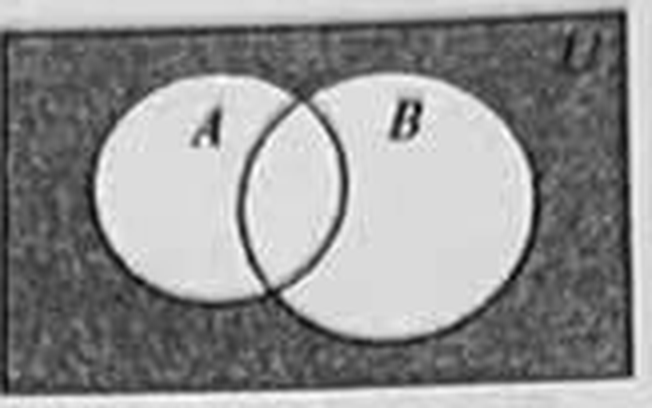
\includegraphics[width=0.30\textwidth]{figures/venn_AB_complement.png}
\end{center}

\ans{$\overline{A\cup B}$}

\ifanswer
\solbegin
\step{图中阴影部分在集合 $A$、$B$ 的外部，即在全集 $U$ 中但不属于 $A$、也不属于 $B$.}
\step{这正是 $A\cup B$ 在全集 $U$ 中的补集，故可表示为 $\overline{A\cup B}$（即 $\complement_U(A\cup B)$）.}
\solend

\fi

\item 设全集 $U=\R$，集合 $A=\{x\mid 2\leqslant x<5\}$，$B=\{x\mid 3<x<6\}$，则 $\overline{A}\cap B=$ \blankline[4.4em]（用区间表示）.

\ans{$[5,6)$}

\ifanswer
\solbegin
\step{在全集 $\R$ 中，$\overline{A}=(-\infty,2)\cup[5,+\infty)$.}
\step{又 $B=(3,6)$，取两集合的公共部分得 $\overline{A}\cap B=[5,6)$.}
\solend

\fi

\item 用反证法证明“$a,b\in\N$，$ab$ 可被 5 整除，那么 $a,b$ 中至少有一个能被 5 整除”时应假设 \blankline[4.4em].

\ans{$a,b$ 都不能被 5 整除}

\ifanswer
\solbegin
\step{反证法需假设结论的反面成立.}
\step{“$a,b$ 中至少有一个能被 5 整除”的反面是“$a,b$ 中没有一个能被 5 整除”，即 $a,b$ 都不能被 5 整除.}
\solend

\fi

\item 满足 $M\subseteq\{a_1,a_2,a_3,a_4,a_5\}$，且 $M\cap\{a_1,a_2,a_3\}=\{a_1,a_2\}$，则集合 $M$ 的个数是 \blankline[2.4em].

\ans{$4$}

\ifanswer
\solbegin
\step{由 $M\cap\{a_1,a_2,a_3\}=\{a_1,a_2\}$ 得 $a_1\in M$，$a_2\in M$，$a_3\notin M$.}
\step{又 $M\subseteq\{a_1,a_2,a_3,a_4,a_5\}$，所以 $a_4$、$a_5$ 可以属于 $M$，也可以不属于 $M$.}
\step{即 $M=\{a_1,a_2\}\cup S$，其中 $S\subseteq\{a_4,a_5\}$，共有 $2^2=4$ 个.}
\solend

\fi

\item 已知集合 $A=\{(x,y)\mid y=x^2\}$，$B=\left\{(x,y)\mid \dfrac{y-1}{x-1}=\dfrac{1}{2}\right\}$，则 $A\cap B=$ \blankline[5.2em].

\ans{$\left\{\left(-\dfrac{1}{2},\dfrac{1}{4}\right)\right\}$}

\ifanswer
\solbegin
\step{集合 $B$ 中的点满足 $y=\dfrac{1}{2}x+\dfrac{1}{2}$，且 $x\neq 1$.}
\step{代入 $y=x^2$ 得 $2x^2-x-1=0$，解得 $x=1$ 或 $x=-\dfrac{1}{2}$.}
\step{因为 $x\neq 1$，所以 $x=-\dfrac{1}{2}$，此时 $y=\dfrac{1}{4}$.}
\step{所以 $A\cap B=\left\{\left(-\dfrac{1}{2},\dfrac{1}{4}\right)\right\}$.}
\solend

\fi

\item 已知集合 $\{a,b,c\}=\{0,1,2\}$，且下列三个关系：①$a\neq 2$ ②$b=2$ ③$c\neq 0$ 有且只有一个正确，则 $100a+10b+c$ 等于 \blankline[2.4em].

\ans{$201$}

\ifanswer
\solbegin
\step{$a,b,c$ 是 $0,1,2$ 的一个排列，共 6 种情形，逐一检验三个关系的真假：}
\step{$(a,b,c)=(0,1,2)$：①真、②假、③真，两个正确，不合；$(0,2,1)$：三个都真，不合；}
\step{$(1,0,2)$：①真、②假、③真，两个正确，不合；$(1,2,0)$：①真、②真、③假，两个正确，不合；}
\step{$(2,0,1)$：①假、②假、③真，恰有一个正确，符合；$(2,1,0)$：三个都假，不合.}
\step{所以 $(a,b,c)=(2,0,1)$，$100a+10b+c=200+0+1=201$.}
\solend

\fi

\item “$x_1>3$ 且 $x_2>3$”是“$x_1+x_2>6$ 且 $x_1x_2>9$”的 \blankline[4.4em] 条件.（选填“充分非必要”，“必要非充分”，“充要”，“既非充分也非必要”）

\ans{充分非必要}

\ifanswer
\solbegin
\step{充分性：若 $x_1>3$ 且 $x_2>3$，则 $x_1+x_2>6$，且 $x_1x_2>9$，故充分性成立.}
\step{必要性：取 $x_1=2$、$x_2=5$，有 $x_1+x_2=7>6$、$x_1x_2=10>9$，但 $x_1>3$ 不成立，故必要性不成立.}
\step{所以应填“充分非必要”.}
\solend

\fi

% 注：第 11 题系 2010 年上海高考理科第 14 题的改写（原题要求选出 4 个子集，官方答案 36）。
%     原题官方解答明言「A、B 可以互换，即视为一种选法」，即**不计先后**计数；
%     按此口径本改写题的答案为 5。（原卷学生作答为 10，是把 A⊆B 与 B⊆A 重复计入。）
\item 在集合 $U=\{a,b,c,d\}$ 的子集中选出 2 个不同的子集，需同时满足以下两个条件：(1)$a,b$ 都要选出 (2)对选出的任意两个子集 $A$ 和 $B$，必有 $A\subseteq B$ 或 $B\subseteq A$，那么共有 \blankline[2.4em] 种不同的选法.

\ans{$5$}

\ifanswer
\solbegin
\step{由 (1) 知 $a,b$ 都要选出，即 $a,b$ 都属于所选的两个子集；由 (2) 知所选的两个子集必须可比.}
\step{含 $a,b$ 的子集只有 $\{a,b\}$、$\{a,b,c\}$、$\{a,b,d\}$、$\{a,b,c,d\}$ 共 4 个.}
\step{在这 4 个子集中取出两个不同的且可比的（一个包含另一个），只有下列 5 组：}
\step{$\{a,b\}\subset\{a,b,c\}$、$\{a,b\}\subset\{a,b,d\}$、$\{a,b\}\subset\{a,b,c,d\}$、$\{a,b,c\}\subset\{a,b,c,d\}$、$\{a,b,d\}\subset\{a,b,c,d\}$.}
\step{注意「选出 2 个子集」的选法\textbf{不计先后}：把这两个子集分别叫作 $A$、$B$ 只是给它们取个名字，$A\subseteq B$ 与 $B\subseteq A$ 说的是同一组子集，算同一种选法.}
\step{（本题由 2010 年上海高考理科第 14 题改写，原题要求选出 4 个子集，其官方答案 36 正是按「$A$、$B$ 可以互换，即视为一种选法」的不计先后口径计数.）}
\step{所以共有 5 种不同的选法.}
\solend

\fi

\end{enumerate}

\bigsec{二、选择题}

\begin{enumerate}
\setcounter{enumi}{11}

\item 已知 $M=(-\infty,\sqrt{3}]$，$a=\sqrt{3}$，则下列关系中正确的是（\quad）.

A. $a\subset M$\qquad B. $a\in M$\qquad C. $\{a\}\in M$\qquad D. $M\subset\{a\}$

\ans{B}

\ifanswer
\solbegin
\step{因为 $\sqrt{3}\leqslant\sqrt{3}$，所以 $a=\sqrt{3}\in M$，B 正确.}
\step{$a$ 是元素、$M$ 是集合，元素与集合之间用 $\in$ 表示，不能用 $\subset$，故 A、D 错误；}
\step{$\{a\}$ 是集合，集合与集合之间应是包含关系（且 $\{a\}\subseteq M$），不能用 $\in$，故 C 错误.}
\step{故选 B.}
\solend

\fi

% 注：原卷此处印作“已知集合{(x,y)|x^2+y^2≤3, x∈Z, y∈Z}”，集合未记作 A，
%     却设问“则 A 中的元素个数是”，显系漏排“A=”；本稿补上，其余照原卷。
\item 已知集合 $A=\{(x,y)\mid x^2+y^2\leqslant 3,\ x\in\Z,\ y\in\Z\}$，则 $A$ 中的元素个数是（\quad）.

A. $9$\qquad B. $8$\qquad C. $5$\qquad D. $4$

\ans{A}

\ifanswer
\solbegin
\step{逐一列举：$x=0$ 时 $y^2\leqslant 3$，$y=-1,0,1$，得 $(0,-1),(0,0),(0,1)$，共 3 个；}
\step{$x=\pm 1$ 时 $y^2\leqslant 2$，$y=-1,0,1$，各得 3 个，共 6 个（$x^2+y^2=2\leqslant 3$ 满足条件）；}
\step{$|x|\geqslant 2$ 时 $x^2\geqslant 4>3$，无解.}
\step{所以 $A$ 中元素个数为 $3+6=9$. 故选 A.}
\solend

\fi

\item 集合 $A=\{x\mid x=(2k-1)\pi,\ k\in\Z\}$ 与 $B=\{x\mid x=(4n\pm 1)\pi,\ n\in\Z\}$ 之间的关系是（\quad）.

A. $A\subset B$\qquad B. $B\subset A$\qquad C. $A=B$\qquad D. 不确定

\ans{C}

\ifanswer
\solbegin
\step{$A$ 由 $\pi$ 的一切奇数倍组成，即 $A=\{\cdots,-3\pi,-\pi,\pi,3\pi,\cdots\}$.}
\step{$B$ 中 $4n+1$ 与 $4n-1$ （$n\in\Z$）都是奇数，故 $B\subseteq A$；}
\step{反之，任一奇数除以 4 的余数只能是 1 或 3：形如 $4m+1$ 的奇数含于 $B$（取 $n=m$），形如 $4m+3=4(m+1)-1$ 的奇数也含于 $B$（取 $n=m+1$），所以 $A\subseteq B$.}
\step{于是 $A\subseteq B$ 且 $B\subseteq A$，即 $A=B$. 故选 C.}
\solend

\fi

\item 设 $T$ 是由正三角形 $P_1P_2P_3$ 边上及其内部的点构成的集合，点 $O$ 是 $\triangle P_1P_2P_3$ 的中心. 若集合 $S=\{P\mid P\in T,\ |PO|\leqslant|PO_i|,\ i=1,2,3\}$，（符号 $|AB|$ 表示平面上两点 $A,B$ 间的距离），则集合 $S$ 表示的平面区域是（\quad）.

A. 四边形区域；\qquad B. 三角形区域；\qquad C. 六边形区域；\qquad D. 五边形区域；

\ans{C}

\ifanswer
\solbegin
\step{$|PO|\leqslant|PO_i|$ 表示点 $P$ 到 $O$ 的距离不大于到顶点 $P_i$ 的距离，即 $P$ 落在线段 $OP_i$ 的垂直平分线靠 $O$ 的那一侧（含该线）.}
\step{对 $i=1,2,3$ 各有一条这样的直线，它们分别把三角形靠近 $P_1$、$P_2$、$P_3$ 的一个小角（三角形）截掉；}
\step{逐一直观验证可知这三条直线两两的交点都在三角形内部，三个角互不重叠，截去三个角后剩下的区域共有 6 条边.}
\step{所以集合 $S$ 表示的平面区域是六边形区域. 故选 C.}
\solend

\fi

\end{enumerate}

\bigsec{三、解答题}

\begin{enumerate}
\setcounter{enumi}{15}

\item（10 分，第 1 小问 5 分，第 2 小问 5 分）已知集合 $A=\{x\mid a\leqslant x\leqslant a+2\}$，集合 $B=\{x\mid x<-1\text{ 或 }x>5\}$，全集 $U=\R$.

\begin{enumerate}[label=(\arabic*)]
\item 若 $a=1$，求 $\overline{A}\cup B$；
\item 若 $A\subseteq B$，求实数 $a$ 的取值范围.
\end{enumerate}

\ans{（1）$(-\infty,1)\cup(3,+\infty)$；（2）$(-\infty,-3)\cup(5,+\infty)$}

\ifanswer
\solbegin
\stepm{(1)}{$a=1$ 时 $A=\{x\mid 1\leqslant x\leqslant 3\}=[1,3]$，则 $\overline{A}=(-\infty,1)\cup(3,+\infty)$.}
\step{又 $B=(-\infty,-1)\cup(5,+\infty)$，而 $B\subseteq\overline{A}$（因 $5>3$、$-1<1$），}
\step{所以 $\overline{A}\cup B=(-\infty,1)\cup(3,+\infty)$.}
\stepm{(2)}{因为 $a\leqslant a+2$，所以集合 $A=\{x\mid a\leqslant x\leqslant a+2\}$ 始终非空.}
\step{要使 $A\subseteq B$，只需 $A$ 与 $[-1,5]$ 没有公共点，即 $a+2<-1$ 或 $a>5$.}
\step{解得 $a<-3$ 或 $a>5$，所以实数 $a$ 的取值范围是 $(-\infty,-3)\cup(5,+\infty)$.}
\solend

\fi

\ansspace[10]

\item（10 分，第 1 小问 5 分，第 2 小问 5 分）已知 $A=\{x\mid x^2+x-2=0\}$，$B=\{x\mid x^2+ax+2a-4=0\}$.

\begin{enumerate}[label=(\arabic*)]
\item 若 $A=B$，求实数 $a$ 的值；
\item 若 $B\subseteq A$，求实数 $a$ 的值.
\end{enumerate}

\ans{（1）$a=1$；（2）$a=1$ 或 $a=4$}

\ifanswer
\solbegin
\stepm{(1)}{由 $x^2+x-2=0$ 解得 $x=1$ 或 $x=-2$，所以 $A=\{1,-2\}$.}
\step{由 $A=B$ 知 $1$、$-2$ 是方程 $x^2+ax+2a-4=0$ 的两根，由根与系数的关系得 $1+(-2)=-a$，所以 $a=1$；}
\step{此时 $2a-4=-2=1\times(-2)$，与两根之积相符，故 $a=1$.}
\stepm{(2)}{方程 $x^2+ax+2a-4=0$ 的判别式 $\Delta=a^2-4(2a-4)=(a-4)^2\geqslant 0$ 恒成立，所以集合 $B$ 不可能是空集.}
\step{由 $B\subseteq A$ 知 $B=\{1\}$ 或 $B=\{-2\}$ 或 $B=\{1,-2\}$.}
\step{若 $B=\{1\}$，则 $1$ 是二重根，$1+1=-a$ 且 $1\times 1=2a-4$，即 $a=-2$ 且 $a=\dfrac{5}{2}$，无解；}
\step{若 $B=\{-2\}$，则 $-2$ 是二重根，$(-2)+(-2)=-a$ 且 $(-2)\times(-2)=2a-4$，两式都给出 $a=4$，符合；}
\step{若 $B=\{1,-2\}$，则 $1+(-2)=-a$，得 $a=1$，此时 $2a-4=-2=1\times(-2)$，符合.}
\step{综上，$a=1$ 或 $a=4$.}
\solend

\fi

\ansspace[12]

\item（11 分，第 1 小问 3 分，第 2 小问 3 分，第 3 小问 5 分）已知非空数集 $S$ 满足：对任意给定的 $x,y\in S$（$x,y$ 可以相同），有 $x+y\in S$ 且 $x-y\in S$.

\begin{enumerate}[label=(\arabic*)]
\item 哪个数一定是 $S$ 中的元素?说明理由；
\item 若 $S$ 是有限集，求 $S$；
\item 若 $S$ 中最小的正数为 5，求 $S$.
\end{enumerate}

\ans{（1）$0$；（2）$S=\{0\}$；（3）$S=\{x\mid x=5a,\ a\in\Z\}$}

\ifanswer
\solbegin
\stepm{(1)}{$0$ 一定是 $S$ 中的元素. 理由：$S$ 非空，取 $x\in S$，在 $x-y\in S$ 中令 $y=x$（$x,y$ 可以相同），得 $x-x=0\in S$.}
\stepm{(2)}{若 $S$ 是有限集，则 $S=\{0\}$. 理由：取 $x\in S$ 且 $x\neq 0$，由 $x+y\in S$ 依次得 $2x=x+x\in S$，$3x=2x+x\in S$，$\cdots$，即 $kx\in S$（$k=1,2,3,\cdots$）；}
\step{这些数互不相同，与 $S$ 是有限集矛盾，所以 $S$ 中除 $0$ 外没有别的元素，即 $S=\{0\}$（此时 $0+0=0\in S$，$0-0=0\in S$，符合条件）.}
\stepm{(3)}{因为 $5\in S$，由 $x+y\in S$ 得 $5+5=10\in S$，$10+5=15\in S$，$\cdots$，故一切正整数倍的 $5$ 都在 $S$ 中；}
\step{又由 $x-y\in S$ 得 $5-5=0\in S$，$0-5=-5\in S$，$-5-5=-10\in S$，$\cdots$，故一切负整数倍的 $5$ 也都在 $S$ 中，即 $\{5a\mid a\in\Z\}\subseteq S$.}
\step{反之，任取 $s\in S$，由 $5\in S$ 及封闭性知 $s-5k\in S$（$k\in\Z$）；把 $s$ 写成 $s=5q+r$（$q\in\Z$，$0\leqslant r<5$），取 $k=q$ 得 $r=s-5q\in S$.}
\step{若 $r>0$，则 $S$ 中有比 $5$ 更小的正数 $r$，与“$S$ 中最小的正数为 5”矛盾，故只能 $r=0$，即 $s=5q$.}
\step{所以 $S=\{x\mid x=5a,\ a\in\Z\}$.}
\solend

\fi

\ansspace[12]

\end{enumerate}

\bigsec{附加题}

\begin{enumerate}
\setcounter{enumi}{18}

\item 已知集合 $A,B,C\subseteq\{1,2,3,\cdots,2024\}$，且 $A\subseteq B\subseteq C$，则有序集合组 $(A,B,C)$ 的个数是 \blankline[3.2em].

\ans{$4^{2024}$}

\ifanswer
\solbegin
\step{对 $U=\{1,2,\cdots,2024\}$ 中的每个元素，它与 $A,B,C$ 的关系只有四种可能：}
\step{在 $A,B,C$ 中都出现；不在 $A$ 中而在 $B,C$ 中出现；只在 $C$ 中出现；在三个集合中都不出现.}
\step{反过来，任取每个元素的一种归属方式，都恰好得到一个满足 $A\subseteq B\subseteq C$ 的有序集合组，故不同的组与不同的归属方式一一对应.}
\step{所以共有 $4\times 4\times\cdots\times 4=4^{2024}$ 个有序集合组.}
\solend

\fi

\item 已知集合 $M=\{1,2,\cdots,10\}$，对它的非空子集 $A$，将 $A$ 中的每个元素 $k$ 都乘以 $(-1)^k$ 再求和，如 $A=\{2,3,6\}$，可求得和为 $(-1)^2\times 2+(-1)^3\times 3+(-1)^6\times 6=5$. 试对 $M$ 的所有非空子集，求这些和的总和 \blankline[3.2em].

\ans{$2560$}

\ifanswer
\solbegin
\step{元素 $k$（$k=1,2,\cdots,10$）出现在 $M$ 的 $2^{9}$ 个非空子集中（其余 9 个元素任取）.}
\step{所以在所有非空子集的和中，$k$ 贡献的总量为 $2^{9}\times(-1)^k\cdot k=512\times(-1)^kk$.}
\step{于是这些和的总和为 $512\displaystyle\sum_{k=1}^{10}(-1)^kk=512\times(-1+2-3+4-5+6-7+8-9+10)=512\times 5=2560$.}
\solend

\fi

\item 设 $a_1,a_2,a_3,a_4$ 是 4 个有理数，使得 $\{a_ia_j\mid 1\leqslant i<j\leqslant 4\}=\left\{-24,-2,-\dfrac{3}{2},-\dfrac{1}{8},1,3\right\}$. 求 $a_1+a_2+a_3+a_4=$ \blankline[3.2em].

\ans{$\pm\dfrac{9}{4}$（两组解，和分别为 $-\dfrac{9}{4}$ 与 $\dfrac{9}{4}$）}

\ifanswer
\solbegin
\step{六个乘积中有 4 个负数、2 个正数. 设 4 个数中正数有 $p$ 个、负数有 $q$ 个（$p+q=4$），则异号的两数相乘得负数，其个数为 $pq$；由 $pq=4$ 得 $p=q=2$，即恰有 2 个正数、2 个负数.}
\step{把 4 个数的绝对值记作 $w,x,y,z>0$，则六个两两乘积的绝对值为 $24,2,\dfrac{3}{2},\dfrac{1}{8},1,3$；其中 $1$ 与 $3$ 来自两对同号的数，$24,2,\dfrac{3}{2},\dfrac{1}{8}$ 来自四对异号的数.}
\step{由 $(a_1a_2a_3a_4)^3=(-24)\times(-2)\times\left(-\dfrac{3}{2}\right)\times\left(-\dfrac{1}{8}\right)\times 1\times 3=27$ 得 $a_1a_2a_3a_4=3$，即去符号后 $wxyz=3$.}
\step{逐一检验可知 $w,x,y,z$ 只能是 $\left\{4,\dfrac{1}{4},6,\dfrac{1}{2}\right\}$：其中 $4\times\dfrac{1}{4}=1$、$6\times\dfrac{1}{2}=3$ 为同号两对的乘积，$4\times 6=24$、$4\times\dfrac{1}{2}=2$、$\dfrac{1}{4}\times 6=\dfrac{3}{2}$、$\dfrac{1}{4}\times\dfrac{1}{2}=\dfrac{1}{8}$ 为异号四对的乘积.}
\step{于是 $\left\{4,\dfrac{1}{4}\right\}$ 中的两个数同号、$\left\{6,\dfrac{1}{2}\right\}$ 中的两个数同号，且这两组异号，得两组解：}
\step{$4,\ \dfrac{1}{4},\ -6,\ -\dfrac{1}{2}$，和为 $-\dfrac{9}{4}$；\quad 或 \quad $6,\ \dfrac{1}{2},\ -4,\ -\dfrac{1}{4}$，和为 $\dfrac{9}{4}$.}
\step{两组解的六个乘积都恰为 $-24,-2,-\dfrac{3}{2},-\dfrac{1}{8},1,3$，与原卷所给集合相同.}
\step{所以 $a_1+a_2+a_3+a_4=\pm\dfrac{9}{4}$.}
\solend

\fi

\end{enumerate}

\end{document}
"
%
% 原始材料为学生作业的手机翻拍照片（卷面为学生本人的**手写作答**，未见教师批改痕迹）。
% 试题文字照原卷录入；答案版给出的是**经核验的正确解答与解析**，与原卷手写答案的差异见 README。
%
% 与原卷的两处排版差异（均已在 README「说明」中交代）：
%   ① 原卷未印分节标题与分值，本稿按题型补「一、填空题 / 二、选择题 / 三、解答题」三节
%      （「附加题」原卷有印）；
%   ② 第 13 题原卷印作「已知集合{(x,y)|…}」，集合未记作 A 却被设问为「A 中的元素个数」，
%      显系漏排「A=」，本稿补上。

% 本篇的正文与家长拍照卷 `高一b_大同中学_第二周周末练习1（补）` **完全相同**——同一份作业，
% 试卷版/答案版也都是同一份源码编译而来；`高一b` 的 4 张原图另存于
% `原图/高一b_大同中学_第二周周末练习1（补）/`，本卷 `原图/` 下是同一组照片的副本。
% 经核对，这份作业就是公众号「魔都数学加油站」连载「27学年高一16——2026-2027年上海市大同中学
% 高一上周末作业2.1」的那一份：**题号与题干逐题一致**，只是公众号版略去了填空第 1、2 题，
% 故拍照卷反而是更完整的版本（对照关系见 README「与公众号连载号的对照表」）。
%
% 本卷的编号与连载号对齐（高一16），卷面标题因此**不带**「（补）」；标题里的「大同中学」为**本稿所加**
% （原卷标题只有作业名，校名只印在页眉「上海市大同…」）。带「（补）」的 `高一b` 保留为
% 拍照原件的转录本，两者内容一字不差。
%
% 一处与公众号讲评版的差异需留意：本卷第 11 题的答案按 2010 年上海高考理科第 14 题官方解答
% 「A、B 可以互换，即视为一种选法」的不计先后口径取 5，而公众号讲评版把它按有先后的 32 计数
% （该题学生原作答为 10）。取舍理由见该题下的 `%` 注。
\documentclass[a4paper,11pt]{article}
\usepackage{common}

\begin{document}

\examtitlest[3]{2026--2027 学年度大同中学高一上数学第二周周末练习1}{集合与常用逻辑用语}

\bigsec{一、填空题}

\begin{enumerate}

\item 用列举法表示集合 $\{x\mid -2<x\leqslant 2,\ x\in\Z\}=$ \blankline[2.4em].

\ans{$\{-1,0,1,2\}$}

\ifanswer
\solbegin
\step{集合中的元素是满足 $-2<x\leqslant 2$ 的整数，即 $-1$、$0$、$1$、$2$.}
\step{所以用列举法表示为 $\{-1,0,1,2\}$.}
\solend

\fi

\item 设集合 $A=\{1,a\}$，$B=\{1,a^2\}$，若 $A=B$，则实数 $a$ 的值为 \blankline[2.4em].

\ans{$a=0$}

\ifanswer
\solbegin
\step{由 $A=B$ 得 $a^2=a$，解得 $a=0$ 或 $a=1$.}
\step{当 $a=1$ 时，$A=\{1,1\}$，不符合集合元素的互异性，舍去；}
\step{当 $a=0$ 时，$A=\{1,0\}$，$B=\{1,0\}$，两集合相等，符合条件.}
\step{所以 $a=0$.}
\solend

\fi

\item 已知集合 $A=\{0,2,3,4,5\}$，$B=\{2,3,5,7\}$，$C=\{2,3,6\}$，则 $(A\cap B)\cup C=$ \blankline[4.4em].

\ans{$\{2,3,5,6\}$}

\ifanswer
\solbegin
\step{$A\cap B=\{0,2,3,4,5\}\cap\{2,3,5,7\}=\{2,3,5\}$.}
\step{所以 $(A\cap B)\cup C=\{2,3,5\}\cup\{2,3,6\}=\{2,3,5,6\}$.}
\solend

\fi

\item 设全集为 $U$，用集合 $A,B$ 的交、并或补集符号表示图中的阴影部分是 \blankline[4.4em].

\begin{center}
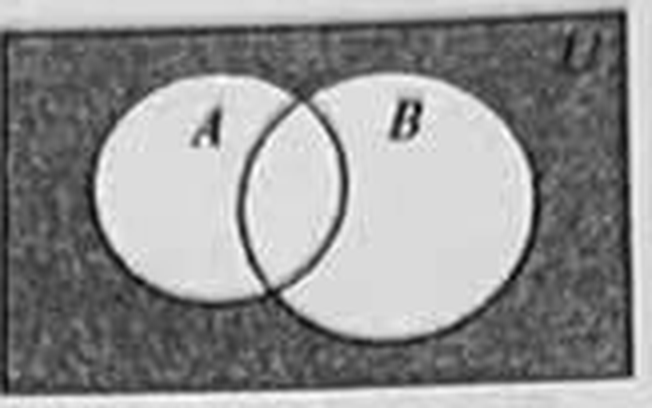
\includegraphics[width=0.30\textwidth]{figures/venn_AB_complement.png}
\end{center}

\ans{$\overline{A\cup B}$}

\ifanswer
\solbegin
\step{图中阴影部分在集合 $A$、$B$ 的外部，即在全集 $U$ 中但不属于 $A$、也不属于 $B$.}
\step{这正是 $A\cup B$ 在全集 $U$ 中的补集，故可表示为 $\overline{A\cup B}$（即 $\complement_U(A\cup B)$）.}
\solend

\fi

\item 设全集 $U=\R$，集合 $A=\{x\mid 2\leqslant x<5\}$，$B=\{x\mid 3<x<6\}$，则 $\overline{A}\cap B=$ \blankline[4.4em]（用区间表示）.

\ans{$[5,6)$}

\ifanswer
\solbegin
\step{在全集 $\R$ 中，$\overline{A}=(-\infty,2)\cup[5,+\infty)$.}
\step{又 $B=(3,6)$，取两集合的公共部分得 $\overline{A}\cap B=[5,6)$.}
\solend

\fi

\item 用反证法证明“$a,b\in\N$，$ab$ 可被 5 整除，那么 $a,b$ 中至少有一个能被 5 整除”时应假设 \blankline[4.4em].

\ans{$a,b$ 都不能被 5 整除}

\ifanswer
\solbegin
\step{反证法需假设结论的反面成立.}
\step{“$a,b$ 中至少有一个能被 5 整除”的反面是“$a,b$ 中没有一个能被 5 整除”，即 $a,b$ 都不能被 5 整除.}
\solend

\fi

\item 满足 $M\subseteq\{a_1,a_2,a_3,a_4,a_5\}$，且 $M\cap\{a_1,a_2,a_3\}=\{a_1,a_2\}$，则集合 $M$ 的个数是 \blankline[2.4em].

\ans{$4$}

\ifanswer
\solbegin
\step{由 $M\cap\{a_1,a_2,a_3\}=\{a_1,a_2\}$ 得 $a_1\in M$，$a_2\in M$，$a_3\notin M$.}
\step{又 $M\subseteq\{a_1,a_2,a_3,a_4,a_5\}$，所以 $a_4$、$a_5$ 可以属于 $M$，也可以不属于 $M$.}
\step{即 $M=\{a_1,a_2\}\cup S$，其中 $S\subseteq\{a_4,a_5\}$，共有 $2^2=4$ 个.}
\solend

\fi

\item 已知集合 $A=\{(x,y)\mid y=x^2\}$，$B=\left\{(x,y)\mid \dfrac{y-1}{x-1}=\dfrac{1}{2}\right\}$，则 $A\cap B=$ \blankline[5.2em].

\ans{$\left\{\left(-\dfrac{1}{2},\dfrac{1}{4}\right)\right\}$}

\ifanswer
\solbegin
\step{集合 $B$ 中的点满足 $y=\dfrac{1}{2}x+\dfrac{1}{2}$，且 $x\neq 1$.}
\step{代入 $y=x^2$ 得 $2x^2-x-1=0$，解得 $x=1$ 或 $x=-\dfrac{1}{2}$.}
\step{因为 $x\neq 1$，所以 $x=-\dfrac{1}{2}$，此时 $y=\dfrac{1}{4}$.}
\step{所以 $A\cap B=\left\{\left(-\dfrac{1}{2},\dfrac{1}{4}\right)\right\}$.}
\solend

\fi

\item 已知集合 $\{a,b,c\}=\{0,1,2\}$，且下列三个关系：①$a\neq 2$ ②$b=2$ ③$c\neq 0$ 有且只有一个正确，则 $100a+10b+c$ 等于 \blankline[2.4em].

\ans{$201$}

\ifanswer
\solbegin
\step{$a,b,c$ 是 $0,1,2$ 的一个排列，共 6 种情形，逐一检验三个关系的真假：}
\step{$(a,b,c)=(0,1,2)$：①真、②假、③真，两个正确，不合；$(0,2,1)$：三个都真，不合；}
\step{$(1,0,2)$：①真、②假、③真，两个正确，不合；$(1,2,0)$：①真、②真、③假，两个正确，不合；}
\step{$(2,0,1)$：①假、②假、③真，恰有一个正确，符合；$(2,1,0)$：三个都假，不合.}
\step{所以 $(a,b,c)=(2,0,1)$，$100a+10b+c=200+0+1=201$.}
\solend

\fi

\item “$x_1>3$ 且 $x_2>3$”是“$x_1+x_2>6$ 且 $x_1x_2>9$”的 \blankline[4.4em] 条件.（选填“充分非必要”，“必要非充分”，“充要”，“既非充分也非必要”）

\ans{充分非必要}

\ifanswer
\solbegin
\step{充分性：若 $x_1>3$ 且 $x_2>3$，则 $x_1+x_2>6$，且 $x_1x_2>9$，故充分性成立.}
\step{必要性：取 $x_1=2$、$x_2=5$，有 $x_1+x_2=7>6$、$x_1x_2=10>9$，但 $x_1>3$ 不成立，故必要性不成立.}
\step{所以应填“充分非必要”.}
\solend

\fi

% 注：第 11 题系 2010 年上海高考理科第 14 题的改写（原题要求选出 4 个子集，官方答案 36）。
%     原题官方解答明言「A、B 可以互换，即视为一种选法」，即**不计先后**计数；
%     按此口径本改写题的答案为 5。（原卷学生作答为 10，是把 A⊆B 与 B⊆A 重复计入。）
\item 在集合 $U=\{a,b,c,d\}$ 的子集中选出 2 个不同的子集，需同时满足以下两个条件：(1)$a,b$ 都要选出 (2)对选出的任意两个子集 $A$ 和 $B$，必有 $A\subseteq B$ 或 $B\subseteq A$，那么共有 \blankline[2.4em] 种不同的选法.

\ans{$5$}

\ifanswer
\solbegin
\step{由 (1) 知 $a,b$ 都要选出，即 $a,b$ 都属于所选的两个子集；由 (2) 知所选的两个子集必须可比.}
\step{含 $a,b$ 的子集只有 $\{a,b\}$、$\{a,b,c\}$、$\{a,b,d\}$、$\{a,b,c,d\}$ 共 4 个.}
\step{在这 4 个子集中取出两个不同的且可比的（一个包含另一个），只有下列 5 组：}
\step{$\{a,b\}\subset\{a,b,c\}$、$\{a,b\}\subset\{a,b,d\}$、$\{a,b\}\subset\{a,b,c,d\}$、$\{a,b,c\}\subset\{a,b,c,d\}$、$\{a,b,d\}\subset\{a,b,c,d\}$.}
\step{注意「选出 2 个子集」的选法\textbf{不计先后}：把这两个子集分别叫作 $A$、$B$ 只是给它们取个名字，$A\subseteq B$ 与 $B\subseteq A$ 说的是同一组子集，算同一种选法.}
\step{（本题由 2010 年上海高考理科第 14 题改写，原题要求选出 4 个子集，其官方答案 36 正是按「$A$、$B$ 可以互换，即视为一种选法」的不计先后口径计数.）}
\step{所以共有 5 种不同的选法.}
\solend

\fi

\end{enumerate}

\bigsec{二、选择题}

\begin{enumerate}
\setcounter{enumi}{11}

\item 已知 $M=(-\infty,\sqrt{3}]$，$a=\sqrt{3}$，则下列关系中正确的是（\quad）.

A. $a\subset M$\qquad B. $a\in M$\qquad C. $\{a\}\in M$\qquad D. $M\subset\{a\}$

\ans{B}

\ifanswer
\solbegin
\step{因为 $\sqrt{3}\leqslant\sqrt{3}$，所以 $a=\sqrt{3}\in M$，B 正确.}
\step{$a$ 是元素、$M$ 是集合，元素与集合之间用 $\in$ 表示，不能用 $\subset$，故 A、D 错误；}
\step{$\{a\}$ 是集合，集合与集合之间应是包含关系（且 $\{a\}\subseteq M$），不能用 $\in$，故 C 错误.}
\step{故选 B.}
\solend

\fi

% 注：原卷此处印作“已知集合{(x,y)|x^2+y^2≤3, x∈Z, y∈Z}”，集合未记作 A，
%     却设问“则 A 中的元素个数是”，显系漏排“A=”；本稿补上，其余照原卷。
\item 已知集合 $A=\{(x,y)\mid x^2+y^2\leqslant 3,\ x\in\Z,\ y\in\Z\}$，则 $A$ 中的元素个数是（\quad）.

A. $9$\qquad B. $8$\qquad C. $5$\qquad D. $4$

\ans{A}

\ifanswer
\solbegin
\step{逐一列举：$x=0$ 时 $y^2\leqslant 3$，$y=-1,0,1$，得 $(0,-1),(0,0),(0,1)$，共 3 个；}
\step{$x=\pm 1$ 时 $y^2\leqslant 2$，$y=-1,0,1$，各得 3 个，共 6 个（$x^2+y^2=2\leqslant 3$ 满足条件）；}
\step{$|x|\geqslant 2$ 时 $x^2\geqslant 4>3$，无解.}
\step{所以 $A$ 中元素个数为 $3+6=9$. 故选 A.}
\solend

\fi

\item 集合 $A=\{x\mid x=(2k-1)\pi,\ k\in\Z\}$ 与 $B=\{x\mid x=(4n\pm 1)\pi,\ n\in\Z\}$ 之间的关系是（\quad）.

A. $A\subset B$\qquad B. $B\subset A$\qquad C. $A=B$\qquad D. 不确定

\ans{C}

\ifanswer
\solbegin
\step{$A$ 由 $\pi$ 的一切奇数倍组成，即 $A=\{\cdots,-3\pi,-\pi,\pi,3\pi,\cdots\}$.}
\step{$B$ 中 $4n+1$ 与 $4n-1$ （$n\in\Z$）都是奇数，故 $B\subseteq A$；}
\step{反之，任一奇数除以 4 的余数只能是 1 或 3：形如 $4m+1$ 的奇数含于 $B$（取 $n=m$），形如 $4m+3=4(m+1)-1$ 的奇数也含于 $B$（取 $n=m+1$），所以 $A\subseteq B$.}
\step{于是 $A\subseteq B$ 且 $B\subseteq A$，即 $A=B$. 故选 C.}
\solend

\fi

\item 设 $T$ 是由正三角形 $P_1P_2P_3$ 边上及其内部的点构成的集合，点 $O$ 是 $\triangle P_1P_2P_3$ 的中心. 若集合 $S=\{P\mid P\in T,\ |PO|\leqslant|PO_i|,\ i=1,2,3\}$，（符号 $|AB|$ 表示平面上两点 $A,B$ 间的距离），则集合 $S$ 表示的平面区域是（\quad）.

A. 四边形区域；\qquad B. 三角形区域；\qquad C. 六边形区域；\qquad D. 五边形区域；

\ans{C}

\ifanswer
\solbegin
\step{$|PO|\leqslant|PO_i|$ 表示点 $P$ 到 $O$ 的距离不大于到顶点 $P_i$ 的距离，即 $P$ 落在线段 $OP_i$ 的垂直平分线靠 $O$ 的那一侧（含该线）.}
\step{对 $i=1,2,3$ 各有一条这样的直线，它们分别把三角形靠近 $P_1$、$P_2$、$P_3$ 的一个小角（三角形）截掉；}
\step{逐一直观验证可知这三条直线两两的交点都在三角形内部，三个角互不重叠，截去三个角后剩下的区域共有 6 条边.}
\step{所以集合 $S$ 表示的平面区域是六边形区域. 故选 C.}
\solend

\fi

\end{enumerate}

\bigsec{三、解答题}

\begin{enumerate}
\setcounter{enumi}{15}

\item（10 分，第 1 小问 5 分，第 2 小问 5 分）已知集合 $A=\{x\mid a\leqslant x\leqslant a+2\}$，集合 $B=\{x\mid x<-1\text{ 或 }x>5\}$，全集 $U=\R$.

\begin{enumerate}[label=(\arabic*)]
\item 若 $a=1$，求 $\overline{A}\cup B$；
\item 若 $A\subseteq B$，求实数 $a$ 的取值范围.
\end{enumerate}

\ans{（1）$(-\infty,1)\cup(3,+\infty)$；（2）$(-\infty,-3)\cup(5,+\infty)$}

\ifanswer
\solbegin
\stepm{(1)}{$a=1$ 时 $A=\{x\mid 1\leqslant x\leqslant 3\}=[1,3]$，则 $\overline{A}=(-\infty,1)\cup(3,+\infty)$.}
\step{又 $B=(-\infty,-1)\cup(5,+\infty)$，而 $B\subseteq\overline{A}$（因 $5>3$、$-1<1$），}
\step{所以 $\overline{A}\cup B=(-\infty,1)\cup(3,+\infty)$.}
\stepm{(2)}{因为 $a\leqslant a+2$，所以集合 $A=\{x\mid a\leqslant x\leqslant a+2\}$ 始终非空.}
\step{要使 $A\subseteq B$，只需 $A$ 与 $[-1,5]$ 没有公共点，即 $a+2<-1$ 或 $a>5$.}
\step{解得 $a<-3$ 或 $a>5$，所以实数 $a$ 的取值范围是 $(-\infty,-3)\cup(5,+\infty)$.}
\solend

\fi

\ansspace[10]

\item（10 分，第 1 小问 5 分，第 2 小问 5 分）已知 $A=\{x\mid x^2+x-2=0\}$，$B=\{x\mid x^2+ax+2a-4=0\}$.

\begin{enumerate}[label=(\arabic*)]
\item 若 $A=B$，求实数 $a$ 的值；
\item 若 $B\subseteq A$，求实数 $a$ 的值.
\end{enumerate}

\ans{（1）$a=1$；（2）$a=1$ 或 $a=4$}

\ifanswer
\solbegin
\stepm{(1)}{由 $x^2+x-2=0$ 解得 $x=1$ 或 $x=-2$，所以 $A=\{1,-2\}$.}
\step{由 $A=B$ 知 $1$、$-2$ 是方程 $x^2+ax+2a-4=0$ 的两根，由根与系数的关系得 $1+(-2)=-a$，所以 $a=1$；}
\step{此时 $2a-4=-2=1\times(-2)$，与两根之积相符，故 $a=1$.}
\stepm{(2)}{方程 $x^2+ax+2a-4=0$ 的判别式 $\Delta=a^2-4(2a-4)=(a-4)^2\geqslant 0$ 恒成立，所以集合 $B$ 不可能是空集.}
\step{由 $B\subseteq A$ 知 $B=\{1\}$ 或 $B=\{-2\}$ 或 $B=\{1,-2\}$.}
\step{若 $B=\{1\}$，则 $1$ 是二重根，$1+1=-a$ 且 $1\times 1=2a-4$，即 $a=-2$ 且 $a=\dfrac{5}{2}$，无解；}
\step{若 $B=\{-2\}$，则 $-2$ 是二重根，$(-2)+(-2)=-a$ 且 $(-2)\times(-2)=2a-4$，两式都给出 $a=4$，符合；}
\step{若 $B=\{1,-2\}$，则 $1+(-2)=-a$，得 $a=1$，此时 $2a-4=-2=1\times(-2)$，符合.}
\step{综上，$a=1$ 或 $a=4$.}
\solend

\fi

\ansspace[12]

\item（11 分，第 1 小问 3 分，第 2 小问 3 分，第 3 小问 5 分）已知非空数集 $S$ 满足：对任意给定的 $x,y\in S$（$x,y$ 可以相同），有 $x+y\in S$ 且 $x-y\in S$.

\begin{enumerate}[label=(\arabic*)]
\item 哪个数一定是 $S$ 中的元素?说明理由；
\item 若 $S$ 是有限集，求 $S$；
\item 若 $S$ 中最小的正数为 5，求 $S$.
\end{enumerate}

\ans{（1）$0$；（2）$S=\{0\}$；（3）$S=\{x\mid x=5a,\ a\in\Z\}$}

\ifanswer
\solbegin
\stepm{(1)}{$0$ 一定是 $S$ 中的元素. 理由：$S$ 非空，取 $x\in S$，在 $x-y\in S$ 中令 $y=x$（$x,y$ 可以相同），得 $x-x=0\in S$.}
\stepm{(2)}{若 $S$ 是有限集，则 $S=\{0\}$. 理由：取 $x\in S$ 且 $x\neq 0$，由 $x+y\in S$ 依次得 $2x=x+x\in S$，$3x=2x+x\in S$，$\cdots$，即 $kx\in S$（$k=1,2,3,\cdots$）；}
\step{这些数互不相同，与 $S$ 是有限集矛盾，所以 $S$ 中除 $0$ 外没有别的元素，即 $S=\{0\}$（此时 $0+0=0\in S$，$0-0=0\in S$，符合条件）.}
\stepm{(3)}{因为 $5\in S$，由 $x+y\in S$ 得 $5+5=10\in S$，$10+5=15\in S$，$\cdots$，故一切正整数倍的 $5$ 都在 $S$ 中；}
\step{又由 $x-y\in S$ 得 $5-5=0\in S$，$0-5=-5\in S$，$-5-5=-10\in S$，$\cdots$，故一切负整数倍的 $5$ 也都在 $S$ 中，即 $\{5a\mid a\in\Z\}\subseteq S$.}
\step{反之，任取 $s\in S$，由 $5\in S$ 及封闭性知 $s-5k\in S$（$k\in\Z$）；把 $s$ 写成 $s=5q+r$（$q\in\Z$，$0\leqslant r<5$），取 $k=q$ 得 $r=s-5q\in S$.}
\step{若 $r>0$，则 $S$ 中有比 $5$ 更小的正数 $r$，与“$S$ 中最小的正数为 5”矛盾，故只能 $r=0$，即 $s=5q$.}
\step{所以 $S=\{x\mid x=5a,\ a\in\Z\}$.}
\solend

\fi

\ansspace[12]

\end{enumerate}

\bigsec{附加题}

\begin{enumerate}
\setcounter{enumi}{18}

\item 已知集合 $A,B,C\subseteq\{1,2,3,\cdots,2024\}$，且 $A\subseteq B\subseteq C$，则有序集合组 $(A,B,C)$ 的个数是 \blankline[3.2em].

\ans{$4^{2024}$}

\ifanswer
\solbegin
\step{对 $U=\{1,2,\cdots,2024\}$ 中的每个元素，它与 $A,B,C$ 的关系只有四种可能：}
\step{在 $A,B,C$ 中都出现；不在 $A$ 中而在 $B,C$ 中出现；只在 $C$ 中出现；在三个集合中都不出现.}
\step{反过来，任取每个元素的一种归属方式，都恰好得到一个满足 $A\subseteq B\subseteq C$ 的有序集合组，故不同的组与不同的归属方式一一对应.}
\step{所以共有 $4\times 4\times\cdots\times 4=4^{2024}$ 个有序集合组.}
\solend

\fi

\item 已知集合 $M=\{1,2,\cdots,10\}$，对它的非空子集 $A$，将 $A$ 中的每个元素 $k$ 都乘以 $(-1)^k$ 再求和，如 $A=\{2,3,6\}$，可求得和为 $(-1)^2\times 2+(-1)^3\times 3+(-1)^6\times 6=5$. 试对 $M$ 的所有非空子集，求这些和的总和 \blankline[3.2em].

\ans{$2560$}

\ifanswer
\solbegin
\step{元素 $k$（$k=1,2,\cdots,10$）出现在 $M$ 的 $2^{9}$ 个非空子集中（其余 9 个元素任取）.}
\step{所以在所有非空子集的和中，$k$ 贡献的总量为 $2^{9}\times(-1)^k\cdot k=512\times(-1)^kk$.}
\step{于是这些和的总和为 $512\displaystyle\sum_{k=1}^{10}(-1)^kk=512\times(-1+2-3+4-5+6-7+8-9+10)=512\times 5=2560$.}
\solend

\fi

\item 设 $a_1,a_2,a_3,a_4$ 是 4 个有理数，使得 $\{a_ia_j\mid 1\leqslant i<j\leqslant 4\}=\left\{-24,-2,-\dfrac{3}{2},-\dfrac{1}{8},1,3\right\}$. 求 $a_1+a_2+a_3+a_4=$ \blankline[3.2em].

\ans{$\pm\dfrac{9}{4}$（两组解，和分别为 $-\dfrac{9}{4}$ 与 $\dfrac{9}{4}$）}

\ifanswer
\solbegin
\step{六个乘积中有 4 个负数、2 个正数. 设 4 个数中正数有 $p$ 个、负数有 $q$ 个（$p+q=4$），则异号的两数相乘得负数，其个数为 $pq$；由 $pq=4$ 得 $p=q=2$，即恰有 2 个正数、2 个负数.}
\step{把 4 个数的绝对值记作 $w,x,y,z>0$，则六个两两乘积的绝对值为 $24,2,\dfrac{3}{2},\dfrac{1}{8},1,3$；其中 $1$ 与 $3$ 来自两对同号的数，$24,2,\dfrac{3}{2},\dfrac{1}{8}$ 来自四对异号的数.}
\step{由 $(a_1a_2a_3a_4)^3=(-24)\times(-2)\times\left(-\dfrac{3}{2}\right)\times\left(-\dfrac{1}{8}\right)\times 1\times 3=27$ 得 $a_1a_2a_3a_4=3$，即去符号后 $wxyz=3$.}
\step{逐一检验可知 $w,x,y,z$ 只能是 $\left\{4,\dfrac{1}{4},6,\dfrac{1}{2}\right\}$：其中 $4\times\dfrac{1}{4}=1$、$6\times\dfrac{1}{2}=3$ 为同号两对的乘积，$4\times 6=24$、$4\times\dfrac{1}{2}=2$、$\dfrac{1}{4}\times 6=\dfrac{3}{2}$、$\dfrac{1}{4}\times\dfrac{1}{2}=\dfrac{1}{8}$ 为异号四对的乘积.}
\step{于是 $\left\{4,\dfrac{1}{4}\right\}$ 中的两个数同号、$\left\{6,\dfrac{1}{2}\right\}$ 中的两个数同号，且这两组异号，得两组解：}
\step{$4,\ \dfrac{1}{4},\ -6,\ -\dfrac{1}{2}$，和为 $-\dfrac{9}{4}$；\quad 或 \quad $6,\ \dfrac{1}{2},\ -4,\ -\dfrac{1}{4}$，和为 $\dfrac{9}{4}$.}
\step{两组解的六个乘积都恰为 $-24,-2,-\dfrac{3}{2},-\dfrac{1}{8},1,3$，与原卷所给集合相同.}
\step{所以 $a_1+a_2+a_3+a_4=\pm\dfrac{9}{4}$.}
\solend

\fi

\end{enumerate}

\end{document}
"
% 紧凑版：xelatex "\def\iscompact{1}% 高一16_大同中学_第二周周末练习1.tex —— 高一上数学「第二周周末练习1」（试卷版/答案版）
% 试卷版：xelatex 高一16_大同中学_第二周周末练习1.tex
% 答案版：xelatex "\def\isanswer{1}% 高一16_大同中学_第二周周末练习1.tex —— 高一上数学「第二周周末练习1」（试卷版/答案版）
% 试卷版：xelatex 高一16_大同中学_第二周周末练习1.tex
% 答案版：xelatex "\def\isanswer{1}% 高一16_大同中学_第二周周末练习1.tex —— 高一上数学「第二周周末练习1」（试卷版/答案版）
% 试卷版：xelatex 高一16_大同中学_第二周周末练习1.tex
% 答案版：xelatex "\def\isanswer{1}\input{高一16_大同中学_第二周周末练习1.tex}"
% 紧凑版：xelatex "\def\iscompact{1}\input{高一16_大同中学_第二周周末练习1.tex}"
%
% 原始材料为学生作业的手机翻拍照片（卷面为学生本人的**手写作答**，未见教师批改痕迹）。
% 试题文字照原卷录入；答案版给出的是**经核验的正确解答与解析**，与原卷手写答案的差异见 README。
%
% 与原卷的两处排版差异（均已在 README「说明」中交代）：
%   ① 原卷未印分节标题与分值，本稿按题型补「一、填空题 / 二、选择题 / 三、解答题」三节
%      （「附加题」原卷有印）；
%   ② 第 13 题原卷印作「已知集合{(x,y)|…}」，集合未记作 A 却被设问为「A 中的元素个数」，
%      显系漏排「A=」，本稿补上。

% 本篇的正文与家长拍照卷 `高一b_大同中学_第二周周末练习1（补）` **完全相同**——同一份作业，
% 试卷版/答案版也都是同一份源码编译而来；`高一b` 的 4 张原图另存于
% `原图/高一b_大同中学_第二周周末练习1（补）/`，本卷 `原图/` 下是同一组照片的副本。
% 经核对，这份作业就是公众号「魔都数学加油站」连载「27学年高一16——2026-2027年上海市大同中学
% 高一上周末作业2.1」的那一份：**题号与题干逐题一致**，只是公众号版略去了填空第 1、2 题，
% 故拍照卷反而是更完整的版本（对照关系见 README「与公众号连载号的对照表」）。
%
% 本卷的编号与连载号对齐（高一16），卷面标题因此**不带**「（补）」；标题里的「大同中学」为**本稿所加**
% （原卷标题只有作业名，校名只印在页眉「上海市大同…」）。带「（补）」的 `高一b` 保留为
% 拍照原件的转录本，两者内容一字不差。
%
% 一处与公众号讲评版的差异需留意：本卷第 11 题的答案按 2010 年上海高考理科第 14 题官方解答
% 「A、B 可以互换，即视为一种选法」的不计先后口径取 5，而公众号讲评版把它按有先后的 32 计数
% （该题学生原作答为 10）。取舍理由见该题下的 `%` 注。
\documentclass[a4paper,11pt]{article}
\usepackage{common}

\begin{document}

\examtitlest[3]{2026--2027 学年度大同中学高一上数学第二周周末练习1}{集合与常用逻辑用语}

\bigsec{一、填空题}

\begin{enumerate}

\item 用列举法表示集合 $\{x\mid -2<x\leqslant 2,\ x\in\Z\}=$ \blankline[2.4em].

\ans{$\{-1,0,1,2\}$}

\ifanswer
\solbegin
\step{集合中的元素是满足 $-2<x\leqslant 2$ 的整数，即 $-1$、$0$、$1$、$2$.}
\step{所以用列举法表示为 $\{-1,0,1,2\}$.}
\solend

\fi

\item 设集合 $A=\{1,a\}$，$B=\{1,a^2\}$，若 $A=B$，则实数 $a$ 的值为 \blankline[2.4em].

\ans{$a=0$}

\ifanswer
\solbegin
\step{由 $A=B$ 得 $a^2=a$，解得 $a=0$ 或 $a=1$.}
\step{当 $a=1$ 时，$A=\{1,1\}$，不符合集合元素的互异性，舍去；}
\step{当 $a=0$ 时，$A=\{1,0\}$，$B=\{1,0\}$，两集合相等，符合条件.}
\step{所以 $a=0$.}
\solend

\fi

\item 已知集合 $A=\{0,2,3,4,5\}$，$B=\{2,3,5,7\}$，$C=\{2,3,6\}$，则 $(A\cap B)\cup C=$ \blankline[4.4em].

\ans{$\{2,3,5,6\}$}

\ifanswer
\solbegin
\step{$A\cap B=\{0,2,3,4,5\}\cap\{2,3,5,7\}=\{2,3,5\}$.}
\step{所以 $(A\cap B)\cup C=\{2,3,5\}\cup\{2,3,6\}=\{2,3,5,6\}$.}
\solend

\fi

\item 设全集为 $U$，用集合 $A,B$ 的交、并或补集符号表示图中的阴影部分是 \blankline[4.4em].

\begin{center}
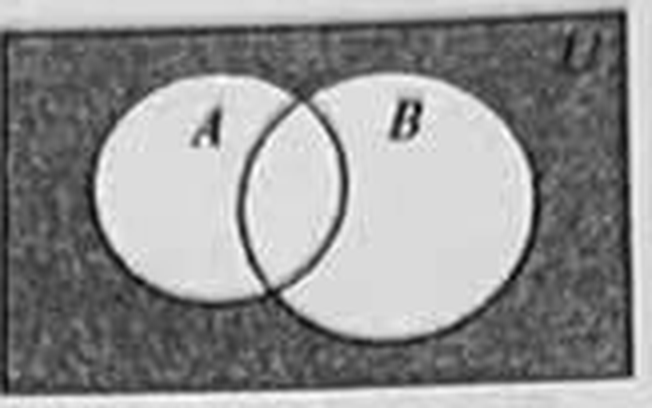
\includegraphics[width=0.30\textwidth]{figures/venn_AB_complement.png}
\end{center}

\ans{$\overline{A\cup B}$}

\ifanswer
\solbegin
\step{图中阴影部分在集合 $A$、$B$ 的外部，即在全集 $U$ 中但不属于 $A$、也不属于 $B$.}
\step{这正是 $A\cup B$ 在全集 $U$ 中的补集，故可表示为 $\overline{A\cup B}$（即 $\complement_U(A\cup B)$）.}
\solend

\fi

\item 设全集 $U=\R$，集合 $A=\{x\mid 2\leqslant x<5\}$，$B=\{x\mid 3<x<6\}$，则 $\overline{A}\cap B=$ \blankline[4.4em]（用区间表示）.

\ans{$[5,6)$}

\ifanswer
\solbegin
\step{在全集 $\R$ 中，$\overline{A}=(-\infty,2)\cup[5,+\infty)$.}
\step{又 $B=(3,6)$，取两集合的公共部分得 $\overline{A}\cap B=[5,6)$.}
\solend

\fi

\item 用反证法证明“$a,b\in\N$，$ab$ 可被 5 整除，那么 $a,b$ 中至少有一个能被 5 整除”时应假设 \blankline[4.4em].

\ans{$a,b$ 都不能被 5 整除}

\ifanswer
\solbegin
\step{反证法需假设结论的反面成立.}
\step{“$a,b$ 中至少有一个能被 5 整除”的反面是“$a,b$ 中没有一个能被 5 整除”，即 $a,b$ 都不能被 5 整除.}
\solend

\fi

\item 满足 $M\subseteq\{a_1,a_2,a_3,a_4,a_5\}$，且 $M\cap\{a_1,a_2,a_3\}=\{a_1,a_2\}$，则集合 $M$ 的个数是 \blankline[2.4em].

\ans{$4$}

\ifanswer
\solbegin
\step{由 $M\cap\{a_1,a_2,a_3\}=\{a_1,a_2\}$ 得 $a_1\in M$，$a_2\in M$，$a_3\notin M$.}
\step{又 $M\subseteq\{a_1,a_2,a_3,a_4,a_5\}$，所以 $a_4$、$a_5$ 可以属于 $M$，也可以不属于 $M$.}
\step{即 $M=\{a_1,a_2\}\cup S$，其中 $S\subseteq\{a_4,a_5\}$，共有 $2^2=4$ 个.}
\solend

\fi

\item 已知集合 $A=\{(x,y)\mid y=x^2\}$，$B=\left\{(x,y)\mid \dfrac{y-1}{x-1}=\dfrac{1}{2}\right\}$，则 $A\cap B=$ \blankline[5.2em].

\ans{$\left\{\left(-\dfrac{1}{2},\dfrac{1}{4}\right)\right\}$}

\ifanswer
\solbegin
\step{集合 $B$ 中的点满足 $y=\dfrac{1}{2}x+\dfrac{1}{2}$，且 $x\neq 1$.}
\step{代入 $y=x^2$ 得 $2x^2-x-1=0$，解得 $x=1$ 或 $x=-\dfrac{1}{2}$.}
\step{因为 $x\neq 1$，所以 $x=-\dfrac{1}{2}$，此时 $y=\dfrac{1}{4}$.}
\step{所以 $A\cap B=\left\{\left(-\dfrac{1}{2},\dfrac{1}{4}\right)\right\}$.}
\solend

\fi

\item 已知集合 $\{a,b,c\}=\{0,1,2\}$，且下列三个关系：①$a\neq 2$ ②$b=2$ ③$c\neq 0$ 有且只有一个正确，则 $100a+10b+c$ 等于 \blankline[2.4em].

\ans{$201$}

\ifanswer
\solbegin
\step{$a,b,c$ 是 $0,1,2$ 的一个排列，共 6 种情形，逐一检验三个关系的真假：}
\step{$(a,b,c)=(0,1,2)$：①真、②假、③真，两个正确，不合；$(0,2,1)$：三个都真，不合；}
\step{$(1,0,2)$：①真、②假、③真，两个正确，不合；$(1,2,0)$：①真、②真、③假，两个正确，不合；}
\step{$(2,0,1)$：①假、②假、③真，恰有一个正确，符合；$(2,1,0)$：三个都假，不合.}
\step{所以 $(a,b,c)=(2,0,1)$，$100a+10b+c=200+0+1=201$.}
\solend

\fi

\item “$x_1>3$ 且 $x_2>3$”是“$x_1+x_2>6$ 且 $x_1x_2>9$”的 \blankline[4.4em] 条件.（选填“充分非必要”，“必要非充分”，“充要”，“既非充分也非必要”）

\ans{充分非必要}

\ifanswer
\solbegin
\step{充分性：若 $x_1>3$ 且 $x_2>3$，则 $x_1+x_2>6$，且 $x_1x_2>9$，故充分性成立.}
\step{必要性：取 $x_1=2$、$x_2=5$，有 $x_1+x_2=7>6$、$x_1x_2=10>9$，但 $x_1>3$ 不成立，故必要性不成立.}
\step{所以应填“充分非必要”.}
\solend

\fi

% 注：第 11 题系 2010 年上海高考理科第 14 题的改写（原题要求选出 4 个子集，官方答案 36）。
%     原题官方解答明言「A、B 可以互换，即视为一种选法」，即**不计先后**计数；
%     按此口径本改写题的答案为 5。（原卷学生作答为 10，是把 A⊆B 与 B⊆A 重复计入。）
\item 在集合 $U=\{a,b,c,d\}$ 的子集中选出 2 个不同的子集，需同时满足以下两个条件：(1)$a,b$ 都要选出 (2)对选出的任意两个子集 $A$ 和 $B$，必有 $A\subseteq B$ 或 $B\subseteq A$，那么共有 \blankline[2.4em] 种不同的选法.

\ans{$5$}

\ifanswer
\solbegin
\step{由 (1) 知 $a,b$ 都要选出，即 $a,b$ 都属于所选的两个子集；由 (2) 知所选的两个子集必须可比.}
\step{含 $a,b$ 的子集只有 $\{a,b\}$、$\{a,b,c\}$、$\{a,b,d\}$、$\{a,b,c,d\}$ 共 4 个.}
\step{在这 4 个子集中取出两个不同的且可比的（一个包含另一个），只有下列 5 组：}
\step{$\{a,b\}\subset\{a,b,c\}$、$\{a,b\}\subset\{a,b,d\}$、$\{a,b\}\subset\{a,b,c,d\}$、$\{a,b,c\}\subset\{a,b,c,d\}$、$\{a,b,d\}\subset\{a,b,c,d\}$.}
\step{注意「选出 2 个子集」的选法\textbf{不计先后}：把这两个子集分别叫作 $A$、$B$ 只是给它们取个名字，$A\subseteq B$ 与 $B\subseteq A$ 说的是同一组子集，算同一种选法.}
\step{（本题由 2010 年上海高考理科第 14 题改写，原题要求选出 4 个子集，其官方答案 36 正是按「$A$、$B$ 可以互换，即视为一种选法」的不计先后口径计数.）}
\step{所以共有 5 种不同的选法.}
\solend

\fi

\end{enumerate}

\bigsec{二、选择题}

\begin{enumerate}
\setcounter{enumi}{11}

\item 已知 $M=(-\infty,\sqrt{3}]$，$a=\sqrt{3}$，则下列关系中正确的是（\quad）.

A. $a\subset M$\qquad B. $a\in M$\qquad C. $\{a\}\in M$\qquad D. $M\subset\{a\}$

\ans{B}

\ifanswer
\solbegin
\step{因为 $\sqrt{3}\leqslant\sqrt{3}$，所以 $a=\sqrt{3}\in M$，B 正确.}
\step{$a$ 是元素、$M$ 是集合，元素与集合之间用 $\in$ 表示，不能用 $\subset$，故 A、D 错误；}
\step{$\{a\}$ 是集合，集合与集合之间应是包含关系（且 $\{a\}\subseteq M$），不能用 $\in$，故 C 错误.}
\step{故选 B.}
\solend

\fi

% 注：原卷此处印作“已知集合{(x,y)|x^2+y^2≤3, x∈Z, y∈Z}”，集合未记作 A，
%     却设问“则 A 中的元素个数是”，显系漏排“A=”；本稿补上，其余照原卷。
\item 已知集合 $A=\{(x,y)\mid x^2+y^2\leqslant 3,\ x\in\Z,\ y\in\Z\}$，则 $A$ 中的元素个数是（\quad）.

A. $9$\qquad B. $8$\qquad C. $5$\qquad D. $4$

\ans{A}

\ifanswer
\solbegin
\step{逐一列举：$x=0$ 时 $y^2\leqslant 3$，$y=-1,0,1$，得 $(0,-1),(0,0),(0,1)$，共 3 个；}
\step{$x=\pm 1$ 时 $y^2\leqslant 2$，$y=-1,0,1$，各得 3 个，共 6 个（$x^2+y^2=2\leqslant 3$ 满足条件）；}
\step{$|x|\geqslant 2$ 时 $x^2\geqslant 4>3$，无解.}
\step{所以 $A$ 中元素个数为 $3+6=9$. 故选 A.}
\solend

\fi

\item 集合 $A=\{x\mid x=(2k-1)\pi,\ k\in\Z\}$ 与 $B=\{x\mid x=(4n\pm 1)\pi,\ n\in\Z\}$ 之间的关系是（\quad）.

A. $A\subset B$\qquad B. $B\subset A$\qquad C. $A=B$\qquad D. 不确定

\ans{C}

\ifanswer
\solbegin
\step{$A$ 由 $\pi$ 的一切奇数倍组成，即 $A=\{\cdots,-3\pi,-\pi,\pi,3\pi,\cdots\}$.}
\step{$B$ 中 $4n+1$ 与 $4n-1$ （$n\in\Z$）都是奇数，故 $B\subseteq A$；}
\step{反之，任一奇数除以 4 的余数只能是 1 或 3：形如 $4m+1$ 的奇数含于 $B$（取 $n=m$），形如 $4m+3=4(m+1)-1$ 的奇数也含于 $B$（取 $n=m+1$），所以 $A\subseteq B$.}
\step{于是 $A\subseteq B$ 且 $B\subseteq A$，即 $A=B$. 故选 C.}
\solend

\fi

\item 设 $T$ 是由正三角形 $P_1P_2P_3$ 边上及其内部的点构成的集合，点 $O$ 是 $\triangle P_1P_2P_3$ 的中心. 若集合 $S=\{P\mid P\in T,\ |PO|\leqslant|PO_i|,\ i=1,2,3\}$，（符号 $|AB|$ 表示平面上两点 $A,B$ 间的距离），则集合 $S$ 表示的平面区域是（\quad）.

A. 四边形区域；\qquad B. 三角形区域；\qquad C. 六边形区域；\qquad D. 五边形区域；

\ans{C}

\ifanswer
\solbegin
\step{$|PO|\leqslant|PO_i|$ 表示点 $P$ 到 $O$ 的距离不大于到顶点 $P_i$ 的距离，即 $P$ 落在线段 $OP_i$ 的垂直平分线靠 $O$ 的那一侧（含该线）.}
\step{对 $i=1,2,3$ 各有一条这样的直线，它们分别把三角形靠近 $P_1$、$P_2$、$P_3$ 的一个小角（三角形）截掉；}
\step{逐一直观验证可知这三条直线两两的交点都在三角形内部，三个角互不重叠，截去三个角后剩下的区域共有 6 条边.}
\step{所以集合 $S$ 表示的平面区域是六边形区域. 故选 C.}
\solend

\fi

\end{enumerate}

\bigsec{三、解答题}

\begin{enumerate}
\setcounter{enumi}{15}

\item（10 分，第 1 小问 5 分，第 2 小问 5 分）已知集合 $A=\{x\mid a\leqslant x\leqslant a+2\}$，集合 $B=\{x\mid x<-1\text{ 或 }x>5\}$，全集 $U=\R$.

\begin{enumerate}[label=(\arabic*)]
\item 若 $a=1$，求 $\overline{A}\cup B$；
\item 若 $A\subseteq B$，求实数 $a$ 的取值范围.
\end{enumerate}

\ans{（1）$(-\infty,1)\cup(3,+\infty)$；（2）$(-\infty,-3)\cup(5,+\infty)$}

\ifanswer
\solbegin
\stepm{(1)}{$a=1$ 时 $A=\{x\mid 1\leqslant x\leqslant 3\}=[1,3]$，则 $\overline{A}=(-\infty,1)\cup(3,+\infty)$.}
\step{又 $B=(-\infty,-1)\cup(5,+\infty)$，而 $B\subseteq\overline{A}$（因 $5>3$、$-1<1$），}
\step{所以 $\overline{A}\cup B=(-\infty,1)\cup(3,+\infty)$.}
\stepm{(2)}{因为 $a\leqslant a+2$，所以集合 $A=\{x\mid a\leqslant x\leqslant a+2\}$ 始终非空.}
\step{要使 $A\subseteq B$，只需 $A$ 与 $[-1,5]$ 没有公共点，即 $a+2<-1$ 或 $a>5$.}
\step{解得 $a<-3$ 或 $a>5$，所以实数 $a$ 的取值范围是 $(-\infty,-3)\cup(5,+\infty)$.}
\solend

\fi

\ansspace[10]

\item（10 分，第 1 小问 5 分，第 2 小问 5 分）已知 $A=\{x\mid x^2+x-2=0\}$，$B=\{x\mid x^2+ax+2a-4=0\}$.

\begin{enumerate}[label=(\arabic*)]
\item 若 $A=B$，求实数 $a$ 的值；
\item 若 $B\subseteq A$，求实数 $a$ 的值.
\end{enumerate}

\ans{（1）$a=1$；（2）$a=1$ 或 $a=4$}

\ifanswer
\solbegin
\stepm{(1)}{由 $x^2+x-2=0$ 解得 $x=1$ 或 $x=-2$，所以 $A=\{1,-2\}$.}
\step{由 $A=B$ 知 $1$、$-2$ 是方程 $x^2+ax+2a-4=0$ 的两根，由根与系数的关系得 $1+(-2)=-a$，所以 $a=1$；}
\step{此时 $2a-4=-2=1\times(-2)$，与两根之积相符，故 $a=1$.}
\stepm{(2)}{方程 $x^2+ax+2a-4=0$ 的判别式 $\Delta=a^2-4(2a-4)=(a-4)^2\geqslant 0$ 恒成立，所以集合 $B$ 不可能是空集.}
\step{由 $B\subseteq A$ 知 $B=\{1\}$ 或 $B=\{-2\}$ 或 $B=\{1,-2\}$.}
\step{若 $B=\{1\}$，则 $1$ 是二重根，$1+1=-a$ 且 $1\times 1=2a-4$，即 $a=-2$ 且 $a=\dfrac{5}{2}$，无解；}
\step{若 $B=\{-2\}$，则 $-2$ 是二重根，$(-2)+(-2)=-a$ 且 $(-2)\times(-2)=2a-4$，两式都给出 $a=4$，符合；}
\step{若 $B=\{1,-2\}$，则 $1+(-2)=-a$，得 $a=1$，此时 $2a-4=-2=1\times(-2)$，符合.}
\step{综上，$a=1$ 或 $a=4$.}
\solend

\fi

\ansspace[12]

\item（11 分，第 1 小问 3 分，第 2 小问 3 分，第 3 小问 5 分）已知非空数集 $S$ 满足：对任意给定的 $x,y\in S$（$x,y$ 可以相同），有 $x+y\in S$ 且 $x-y\in S$.

\begin{enumerate}[label=(\arabic*)]
\item 哪个数一定是 $S$ 中的元素?说明理由；
\item 若 $S$ 是有限集，求 $S$；
\item 若 $S$ 中最小的正数为 5，求 $S$.
\end{enumerate}

\ans{（1）$0$；（2）$S=\{0\}$；（3）$S=\{x\mid x=5a,\ a\in\Z\}$}

\ifanswer
\solbegin
\stepm{(1)}{$0$ 一定是 $S$ 中的元素. 理由：$S$ 非空，取 $x\in S$，在 $x-y\in S$ 中令 $y=x$（$x,y$ 可以相同），得 $x-x=0\in S$.}
\stepm{(2)}{若 $S$ 是有限集，则 $S=\{0\}$. 理由：取 $x\in S$ 且 $x\neq 0$，由 $x+y\in S$ 依次得 $2x=x+x\in S$，$3x=2x+x\in S$，$\cdots$，即 $kx\in S$（$k=1,2,3,\cdots$）；}
\step{这些数互不相同，与 $S$ 是有限集矛盾，所以 $S$ 中除 $0$ 外没有别的元素，即 $S=\{0\}$（此时 $0+0=0\in S$，$0-0=0\in S$，符合条件）.}
\stepm{(3)}{因为 $5\in S$，由 $x+y\in S$ 得 $5+5=10\in S$，$10+5=15\in S$，$\cdots$，故一切正整数倍的 $5$ 都在 $S$ 中；}
\step{又由 $x-y\in S$ 得 $5-5=0\in S$，$0-5=-5\in S$，$-5-5=-10\in S$，$\cdots$，故一切负整数倍的 $5$ 也都在 $S$ 中，即 $\{5a\mid a\in\Z\}\subseteq S$.}
\step{反之，任取 $s\in S$，由 $5\in S$ 及封闭性知 $s-5k\in S$（$k\in\Z$）；把 $s$ 写成 $s=5q+r$（$q\in\Z$，$0\leqslant r<5$），取 $k=q$ 得 $r=s-5q\in S$.}
\step{若 $r>0$，则 $S$ 中有比 $5$ 更小的正数 $r$，与“$S$ 中最小的正数为 5”矛盾，故只能 $r=0$，即 $s=5q$.}
\step{所以 $S=\{x\mid x=5a,\ a\in\Z\}$.}
\solend

\fi

\ansspace[12]

\end{enumerate}

\bigsec{附加题}

\begin{enumerate}
\setcounter{enumi}{18}

\item 已知集合 $A,B,C\subseteq\{1,2,3,\cdots,2024\}$，且 $A\subseteq B\subseteq C$，则有序集合组 $(A,B,C)$ 的个数是 \blankline[3.2em].

\ans{$4^{2024}$}

\ifanswer
\solbegin
\step{对 $U=\{1,2,\cdots,2024\}$ 中的每个元素，它与 $A,B,C$ 的关系只有四种可能：}
\step{在 $A,B,C$ 中都出现；不在 $A$ 中而在 $B,C$ 中出现；只在 $C$ 中出现；在三个集合中都不出现.}
\step{反过来，任取每个元素的一种归属方式，都恰好得到一个满足 $A\subseteq B\subseteq C$ 的有序集合组，故不同的组与不同的归属方式一一对应.}
\step{所以共有 $4\times 4\times\cdots\times 4=4^{2024}$ 个有序集合组.}
\solend

\fi

\item 已知集合 $M=\{1,2,\cdots,10\}$，对它的非空子集 $A$，将 $A$ 中的每个元素 $k$ 都乘以 $(-1)^k$ 再求和，如 $A=\{2,3,6\}$，可求得和为 $(-1)^2\times 2+(-1)^3\times 3+(-1)^6\times 6=5$. 试对 $M$ 的所有非空子集，求这些和的总和 \blankline[3.2em].

\ans{$2560$}

\ifanswer
\solbegin
\step{元素 $k$（$k=1,2,\cdots,10$）出现在 $M$ 的 $2^{9}$ 个非空子集中（其余 9 个元素任取）.}
\step{所以在所有非空子集的和中，$k$ 贡献的总量为 $2^{9}\times(-1)^k\cdot k=512\times(-1)^kk$.}
\step{于是这些和的总和为 $512\displaystyle\sum_{k=1}^{10}(-1)^kk=512\times(-1+2-3+4-5+6-7+8-9+10)=512\times 5=2560$.}
\solend

\fi

\item 设 $a_1,a_2,a_3,a_4$ 是 4 个有理数，使得 $\{a_ia_j\mid 1\leqslant i<j\leqslant 4\}=\left\{-24,-2,-\dfrac{3}{2},-\dfrac{1}{8},1,3\right\}$. 求 $a_1+a_2+a_3+a_4=$ \blankline[3.2em].

\ans{$\pm\dfrac{9}{4}$（两组解，和分别为 $-\dfrac{9}{4}$ 与 $\dfrac{9}{4}$）}

\ifanswer
\solbegin
\step{六个乘积中有 4 个负数、2 个正数. 设 4 个数中正数有 $p$ 个、负数有 $q$ 个（$p+q=4$），则异号的两数相乘得负数，其个数为 $pq$；由 $pq=4$ 得 $p=q=2$，即恰有 2 个正数、2 个负数.}
\step{把 4 个数的绝对值记作 $w,x,y,z>0$，则六个两两乘积的绝对值为 $24,2,\dfrac{3}{2},\dfrac{1}{8},1,3$；其中 $1$ 与 $3$ 来自两对同号的数，$24,2,\dfrac{3}{2},\dfrac{1}{8}$ 来自四对异号的数.}
\step{由 $(a_1a_2a_3a_4)^3=(-24)\times(-2)\times\left(-\dfrac{3}{2}\right)\times\left(-\dfrac{1}{8}\right)\times 1\times 3=27$ 得 $a_1a_2a_3a_4=3$，即去符号后 $wxyz=3$.}
\step{逐一检验可知 $w,x,y,z$ 只能是 $\left\{4,\dfrac{1}{4},6,\dfrac{1}{2}\right\}$：其中 $4\times\dfrac{1}{4}=1$、$6\times\dfrac{1}{2}=3$ 为同号两对的乘积，$4\times 6=24$、$4\times\dfrac{1}{2}=2$、$\dfrac{1}{4}\times 6=\dfrac{3}{2}$、$\dfrac{1}{4}\times\dfrac{1}{2}=\dfrac{1}{8}$ 为异号四对的乘积.}
\step{于是 $\left\{4,\dfrac{1}{4}\right\}$ 中的两个数同号、$\left\{6,\dfrac{1}{2}\right\}$ 中的两个数同号，且这两组异号，得两组解：}
\step{$4,\ \dfrac{1}{4},\ -6,\ -\dfrac{1}{2}$，和为 $-\dfrac{9}{4}$；\quad 或 \quad $6,\ \dfrac{1}{2},\ -4,\ -\dfrac{1}{4}$，和为 $\dfrac{9}{4}$.}
\step{两组解的六个乘积都恰为 $-24,-2,-\dfrac{3}{2},-\dfrac{1}{8},1,3$，与原卷所给集合相同.}
\step{所以 $a_1+a_2+a_3+a_4=\pm\dfrac{9}{4}$.}
\solend

\fi

\end{enumerate}

\end{document}
"
% 紧凑版：xelatex "\def\iscompact{1}% 高一16_大同中学_第二周周末练习1.tex —— 高一上数学「第二周周末练习1」（试卷版/答案版）
% 试卷版：xelatex 高一16_大同中学_第二周周末练习1.tex
% 答案版：xelatex "\def\isanswer{1}\input{高一16_大同中学_第二周周末练习1.tex}"
% 紧凑版：xelatex "\def\iscompact{1}\input{高一16_大同中学_第二周周末练习1.tex}"
%
% 原始材料为学生作业的手机翻拍照片（卷面为学生本人的**手写作答**，未见教师批改痕迹）。
% 试题文字照原卷录入；答案版给出的是**经核验的正确解答与解析**，与原卷手写答案的差异见 README。
%
% 与原卷的两处排版差异（均已在 README「说明」中交代）：
%   ① 原卷未印分节标题与分值，本稿按题型补「一、填空题 / 二、选择题 / 三、解答题」三节
%      （「附加题」原卷有印）；
%   ② 第 13 题原卷印作「已知集合{(x,y)|…}」，集合未记作 A 却被设问为「A 中的元素个数」，
%      显系漏排「A=」，本稿补上。

% 本篇的正文与家长拍照卷 `高一b_大同中学_第二周周末练习1（补）` **完全相同**——同一份作业，
% 试卷版/答案版也都是同一份源码编译而来；`高一b` 的 4 张原图另存于
% `原图/高一b_大同中学_第二周周末练习1（补）/`，本卷 `原图/` 下是同一组照片的副本。
% 经核对，这份作业就是公众号「魔都数学加油站」连载「27学年高一16——2026-2027年上海市大同中学
% 高一上周末作业2.1」的那一份：**题号与题干逐题一致**，只是公众号版略去了填空第 1、2 题，
% 故拍照卷反而是更完整的版本（对照关系见 README「与公众号连载号的对照表」）。
%
% 本卷的编号与连载号对齐（高一16），卷面标题因此**不带**「（补）」；标题里的「大同中学」为**本稿所加**
% （原卷标题只有作业名，校名只印在页眉「上海市大同…」）。带「（补）」的 `高一b` 保留为
% 拍照原件的转录本，两者内容一字不差。
%
% 一处与公众号讲评版的差异需留意：本卷第 11 题的答案按 2010 年上海高考理科第 14 题官方解答
% 「A、B 可以互换，即视为一种选法」的不计先后口径取 5，而公众号讲评版把它按有先后的 32 计数
% （该题学生原作答为 10）。取舍理由见该题下的 `%` 注。
\documentclass[a4paper,11pt]{article}
\usepackage{common}

\begin{document}

\examtitlest[3]{2026--2027 学年度大同中学高一上数学第二周周末练习1}{集合与常用逻辑用语}

\bigsec{一、填空题}

\begin{enumerate}

\item 用列举法表示集合 $\{x\mid -2<x\leqslant 2,\ x\in\Z\}=$ \blankline[2.4em].

\ans{$\{-1,0,1,2\}$}

\ifanswer
\solbegin
\step{集合中的元素是满足 $-2<x\leqslant 2$ 的整数，即 $-1$、$0$、$1$、$2$.}
\step{所以用列举法表示为 $\{-1,0,1,2\}$.}
\solend

\fi

\item 设集合 $A=\{1,a\}$，$B=\{1,a^2\}$，若 $A=B$，则实数 $a$ 的值为 \blankline[2.4em].

\ans{$a=0$}

\ifanswer
\solbegin
\step{由 $A=B$ 得 $a^2=a$，解得 $a=0$ 或 $a=1$.}
\step{当 $a=1$ 时，$A=\{1,1\}$，不符合集合元素的互异性，舍去；}
\step{当 $a=0$ 时，$A=\{1,0\}$，$B=\{1,0\}$，两集合相等，符合条件.}
\step{所以 $a=0$.}
\solend

\fi

\item 已知集合 $A=\{0,2,3,4,5\}$，$B=\{2,3,5,7\}$，$C=\{2,3,6\}$，则 $(A\cap B)\cup C=$ \blankline[4.4em].

\ans{$\{2,3,5,6\}$}

\ifanswer
\solbegin
\step{$A\cap B=\{0,2,3,4,5\}\cap\{2,3,5,7\}=\{2,3,5\}$.}
\step{所以 $(A\cap B)\cup C=\{2,3,5\}\cup\{2,3,6\}=\{2,3,5,6\}$.}
\solend

\fi

\item 设全集为 $U$，用集合 $A,B$ 的交、并或补集符号表示图中的阴影部分是 \blankline[4.4em].

\begin{center}
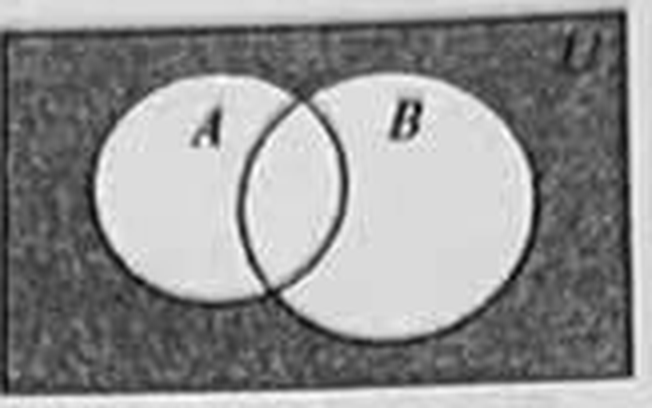
\includegraphics[width=0.30\textwidth]{figures/venn_AB_complement.png}
\end{center}

\ans{$\overline{A\cup B}$}

\ifanswer
\solbegin
\step{图中阴影部分在集合 $A$、$B$ 的外部，即在全集 $U$ 中但不属于 $A$、也不属于 $B$.}
\step{这正是 $A\cup B$ 在全集 $U$ 中的补集，故可表示为 $\overline{A\cup B}$（即 $\complement_U(A\cup B)$）.}
\solend

\fi

\item 设全集 $U=\R$，集合 $A=\{x\mid 2\leqslant x<5\}$，$B=\{x\mid 3<x<6\}$，则 $\overline{A}\cap B=$ \blankline[4.4em]（用区间表示）.

\ans{$[5,6)$}

\ifanswer
\solbegin
\step{在全集 $\R$ 中，$\overline{A}=(-\infty,2)\cup[5,+\infty)$.}
\step{又 $B=(3,6)$，取两集合的公共部分得 $\overline{A}\cap B=[5,6)$.}
\solend

\fi

\item 用反证法证明“$a,b\in\N$，$ab$ 可被 5 整除，那么 $a,b$ 中至少有一个能被 5 整除”时应假设 \blankline[4.4em].

\ans{$a,b$ 都不能被 5 整除}

\ifanswer
\solbegin
\step{反证法需假设结论的反面成立.}
\step{“$a,b$ 中至少有一个能被 5 整除”的反面是“$a,b$ 中没有一个能被 5 整除”，即 $a,b$ 都不能被 5 整除.}
\solend

\fi

\item 满足 $M\subseteq\{a_1,a_2,a_3,a_4,a_5\}$，且 $M\cap\{a_1,a_2,a_3\}=\{a_1,a_2\}$，则集合 $M$ 的个数是 \blankline[2.4em].

\ans{$4$}

\ifanswer
\solbegin
\step{由 $M\cap\{a_1,a_2,a_3\}=\{a_1,a_2\}$ 得 $a_1\in M$，$a_2\in M$，$a_3\notin M$.}
\step{又 $M\subseteq\{a_1,a_2,a_3,a_4,a_5\}$，所以 $a_4$、$a_5$ 可以属于 $M$，也可以不属于 $M$.}
\step{即 $M=\{a_1,a_2\}\cup S$，其中 $S\subseteq\{a_4,a_5\}$，共有 $2^2=4$ 个.}
\solend

\fi

\item 已知集合 $A=\{(x,y)\mid y=x^2\}$，$B=\left\{(x,y)\mid \dfrac{y-1}{x-1}=\dfrac{1}{2}\right\}$，则 $A\cap B=$ \blankline[5.2em].

\ans{$\left\{\left(-\dfrac{1}{2},\dfrac{1}{4}\right)\right\}$}

\ifanswer
\solbegin
\step{集合 $B$ 中的点满足 $y=\dfrac{1}{2}x+\dfrac{1}{2}$，且 $x\neq 1$.}
\step{代入 $y=x^2$ 得 $2x^2-x-1=0$，解得 $x=1$ 或 $x=-\dfrac{1}{2}$.}
\step{因为 $x\neq 1$，所以 $x=-\dfrac{1}{2}$，此时 $y=\dfrac{1}{4}$.}
\step{所以 $A\cap B=\left\{\left(-\dfrac{1}{2},\dfrac{1}{4}\right)\right\}$.}
\solend

\fi

\item 已知集合 $\{a,b,c\}=\{0,1,2\}$，且下列三个关系：①$a\neq 2$ ②$b=2$ ③$c\neq 0$ 有且只有一个正确，则 $100a+10b+c$ 等于 \blankline[2.4em].

\ans{$201$}

\ifanswer
\solbegin
\step{$a,b,c$ 是 $0,1,2$ 的一个排列，共 6 种情形，逐一检验三个关系的真假：}
\step{$(a,b,c)=(0,1,2)$：①真、②假、③真，两个正确，不合；$(0,2,1)$：三个都真，不合；}
\step{$(1,0,2)$：①真、②假、③真，两个正确，不合；$(1,2,0)$：①真、②真、③假，两个正确，不合；}
\step{$(2,0,1)$：①假、②假、③真，恰有一个正确，符合；$(2,1,0)$：三个都假，不合.}
\step{所以 $(a,b,c)=(2,0,1)$，$100a+10b+c=200+0+1=201$.}
\solend

\fi

\item “$x_1>3$ 且 $x_2>3$”是“$x_1+x_2>6$ 且 $x_1x_2>9$”的 \blankline[4.4em] 条件.（选填“充分非必要”，“必要非充分”，“充要”，“既非充分也非必要”）

\ans{充分非必要}

\ifanswer
\solbegin
\step{充分性：若 $x_1>3$ 且 $x_2>3$，则 $x_1+x_2>6$，且 $x_1x_2>9$，故充分性成立.}
\step{必要性：取 $x_1=2$、$x_2=5$，有 $x_1+x_2=7>6$、$x_1x_2=10>9$，但 $x_1>3$ 不成立，故必要性不成立.}
\step{所以应填“充分非必要”.}
\solend

\fi

% 注：第 11 题系 2010 年上海高考理科第 14 题的改写（原题要求选出 4 个子集，官方答案 36）。
%     原题官方解答明言「A、B 可以互换，即视为一种选法」，即**不计先后**计数；
%     按此口径本改写题的答案为 5。（原卷学生作答为 10，是把 A⊆B 与 B⊆A 重复计入。）
\item 在集合 $U=\{a,b,c,d\}$ 的子集中选出 2 个不同的子集，需同时满足以下两个条件：(1)$a,b$ 都要选出 (2)对选出的任意两个子集 $A$ 和 $B$，必有 $A\subseteq B$ 或 $B\subseteq A$，那么共有 \blankline[2.4em] 种不同的选法.

\ans{$5$}

\ifanswer
\solbegin
\step{由 (1) 知 $a,b$ 都要选出，即 $a,b$ 都属于所选的两个子集；由 (2) 知所选的两个子集必须可比.}
\step{含 $a,b$ 的子集只有 $\{a,b\}$、$\{a,b,c\}$、$\{a,b,d\}$、$\{a,b,c,d\}$ 共 4 个.}
\step{在这 4 个子集中取出两个不同的且可比的（一个包含另一个），只有下列 5 组：}
\step{$\{a,b\}\subset\{a,b,c\}$、$\{a,b\}\subset\{a,b,d\}$、$\{a,b\}\subset\{a,b,c,d\}$、$\{a,b,c\}\subset\{a,b,c,d\}$、$\{a,b,d\}\subset\{a,b,c,d\}$.}
\step{注意「选出 2 个子集」的选法\textbf{不计先后}：把这两个子集分别叫作 $A$、$B$ 只是给它们取个名字，$A\subseteq B$ 与 $B\subseteq A$ 说的是同一组子集，算同一种选法.}
\step{（本题由 2010 年上海高考理科第 14 题改写，原题要求选出 4 个子集，其官方答案 36 正是按「$A$、$B$ 可以互换，即视为一种选法」的不计先后口径计数.）}
\step{所以共有 5 种不同的选法.}
\solend

\fi

\end{enumerate}

\bigsec{二、选择题}

\begin{enumerate}
\setcounter{enumi}{11}

\item 已知 $M=(-\infty,\sqrt{3}]$，$a=\sqrt{3}$，则下列关系中正确的是（\quad）.

A. $a\subset M$\qquad B. $a\in M$\qquad C. $\{a\}\in M$\qquad D. $M\subset\{a\}$

\ans{B}

\ifanswer
\solbegin
\step{因为 $\sqrt{3}\leqslant\sqrt{3}$，所以 $a=\sqrt{3}\in M$，B 正确.}
\step{$a$ 是元素、$M$ 是集合，元素与集合之间用 $\in$ 表示，不能用 $\subset$，故 A、D 错误；}
\step{$\{a\}$ 是集合，集合与集合之间应是包含关系（且 $\{a\}\subseteq M$），不能用 $\in$，故 C 错误.}
\step{故选 B.}
\solend

\fi

% 注：原卷此处印作“已知集合{(x,y)|x^2+y^2≤3, x∈Z, y∈Z}”，集合未记作 A，
%     却设问“则 A 中的元素个数是”，显系漏排“A=”；本稿补上，其余照原卷。
\item 已知集合 $A=\{(x,y)\mid x^2+y^2\leqslant 3,\ x\in\Z,\ y\in\Z\}$，则 $A$ 中的元素个数是（\quad）.

A. $9$\qquad B. $8$\qquad C. $5$\qquad D. $4$

\ans{A}

\ifanswer
\solbegin
\step{逐一列举：$x=0$ 时 $y^2\leqslant 3$，$y=-1,0,1$，得 $(0,-1),(0,0),(0,1)$，共 3 个；}
\step{$x=\pm 1$ 时 $y^2\leqslant 2$，$y=-1,0,1$，各得 3 个，共 6 个（$x^2+y^2=2\leqslant 3$ 满足条件）；}
\step{$|x|\geqslant 2$ 时 $x^2\geqslant 4>3$，无解.}
\step{所以 $A$ 中元素个数为 $3+6=9$. 故选 A.}
\solend

\fi

\item 集合 $A=\{x\mid x=(2k-1)\pi,\ k\in\Z\}$ 与 $B=\{x\mid x=(4n\pm 1)\pi,\ n\in\Z\}$ 之间的关系是（\quad）.

A. $A\subset B$\qquad B. $B\subset A$\qquad C. $A=B$\qquad D. 不确定

\ans{C}

\ifanswer
\solbegin
\step{$A$ 由 $\pi$ 的一切奇数倍组成，即 $A=\{\cdots,-3\pi,-\pi,\pi,3\pi,\cdots\}$.}
\step{$B$ 中 $4n+1$ 与 $4n-1$ （$n\in\Z$）都是奇数，故 $B\subseteq A$；}
\step{反之，任一奇数除以 4 的余数只能是 1 或 3：形如 $4m+1$ 的奇数含于 $B$（取 $n=m$），形如 $4m+3=4(m+1)-1$ 的奇数也含于 $B$（取 $n=m+1$），所以 $A\subseteq B$.}
\step{于是 $A\subseteq B$ 且 $B\subseteq A$，即 $A=B$. 故选 C.}
\solend

\fi

\item 设 $T$ 是由正三角形 $P_1P_2P_3$ 边上及其内部的点构成的集合，点 $O$ 是 $\triangle P_1P_2P_3$ 的中心. 若集合 $S=\{P\mid P\in T,\ |PO|\leqslant|PO_i|,\ i=1,2,3\}$，（符号 $|AB|$ 表示平面上两点 $A,B$ 间的距离），则集合 $S$ 表示的平面区域是（\quad）.

A. 四边形区域；\qquad B. 三角形区域；\qquad C. 六边形区域；\qquad D. 五边形区域；

\ans{C}

\ifanswer
\solbegin
\step{$|PO|\leqslant|PO_i|$ 表示点 $P$ 到 $O$ 的距离不大于到顶点 $P_i$ 的距离，即 $P$ 落在线段 $OP_i$ 的垂直平分线靠 $O$ 的那一侧（含该线）.}
\step{对 $i=1,2,3$ 各有一条这样的直线，它们分别把三角形靠近 $P_1$、$P_2$、$P_3$ 的一个小角（三角形）截掉；}
\step{逐一直观验证可知这三条直线两两的交点都在三角形内部，三个角互不重叠，截去三个角后剩下的区域共有 6 条边.}
\step{所以集合 $S$ 表示的平面区域是六边形区域. 故选 C.}
\solend

\fi

\end{enumerate}

\bigsec{三、解答题}

\begin{enumerate}
\setcounter{enumi}{15}

\item（10 分，第 1 小问 5 分，第 2 小问 5 分）已知集合 $A=\{x\mid a\leqslant x\leqslant a+2\}$，集合 $B=\{x\mid x<-1\text{ 或 }x>5\}$，全集 $U=\R$.

\begin{enumerate}[label=(\arabic*)]
\item 若 $a=1$，求 $\overline{A}\cup B$；
\item 若 $A\subseteq B$，求实数 $a$ 的取值范围.
\end{enumerate}

\ans{（1）$(-\infty,1)\cup(3,+\infty)$；（2）$(-\infty,-3)\cup(5,+\infty)$}

\ifanswer
\solbegin
\stepm{(1)}{$a=1$ 时 $A=\{x\mid 1\leqslant x\leqslant 3\}=[1,3]$，则 $\overline{A}=(-\infty,1)\cup(3,+\infty)$.}
\step{又 $B=(-\infty,-1)\cup(5,+\infty)$，而 $B\subseteq\overline{A}$（因 $5>3$、$-1<1$），}
\step{所以 $\overline{A}\cup B=(-\infty,1)\cup(3,+\infty)$.}
\stepm{(2)}{因为 $a\leqslant a+2$，所以集合 $A=\{x\mid a\leqslant x\leqslant a+2\}$ 始终非空.}
\step{要使 $A\subseteq B$，只需 $A$ 与 $[-1,5]$ 没有公共点，即 $a+2<-1$ 或 $a>5$.}
\step{解得 $a<-3$ 或 $a>5$，所以实数 $a$ 的取值范围是 $(-\infty,-3)\cup(5,+\infty)$.}
\solend

\fi

\ansspace[10]

\item（10 分，第 1 小问 5 分，第 2 小问 5 分）已知 $A=\{x\mid x^2+x-2=0\}$，$B=\{x\mid x^2+ax+2a-4=0\}$.

\begin{enumerate}[label=(\arabic*)]
\item 若 $A=B$，求实数 $a$ 的值；
\item 若 $B\subseteq A$，求实数 $a$ 的值.
\end{enumerate}

\ans{（1）$a=1$；（2）$a=1$ 或 $a=4$}

\ifanswer
\solbegin
\stepm{(1)}{由 $x^2+x-2=0$ 解得 $x=1$ 或 $x=-2$，所以 $A=\{1,-2\}$.}
\step{由 $A=B$ 知 $1$、$-2$ 是方程 $x^2+ax+2a-4=0$ 的两根，由根与系数的关系得 $1+(-2)=-a$，所以 $a=1$；}
\step{此时 $2a-4=-2=1\times(-2)$，与两根之积相符，故 $a=1$.}
\stepm{(2)}{方程 $x^2+ax+2a-4=0$ 的判别式 $\Delta=a^2-4(2a-4)=(a-4)^2\geqslant 0$ 恒成立，所以集合 $B$ 不可能是空集.}
\step{由 $B\subseteq A$ 知 $B=\{1\}$ 或 $B=\{-2\}$ 或 $B=\{1,-2\}$.}
\step{若 $B=\{1\}$，则 $1$ 是二重根，$1+1=-a$ 且 $1\times 1=2a-4$，即 $a=-2$ 且 $a=\dfrac{5}{2}$，无解；}
\step{若 $B=\{-2\}$，则 $-2$ 是二重根，$(-2)+(-2)=-a$ 且 $(-2)\times(-2)=2a-4$，两式都给出 $a=4$，符合；}
\step{若 $B=\{1,-2\}$，则 $1+(-2)=-a$，得 $a=1$，此时 $2a-4=-2=1\times(-2)$，符合.}
\step{综上，$a=1$ 或 $a=4$.}
\solend

\fi

\ansspace[12]

\item（11 分，第 1 小问 3 分，第 2 小问 3 分，第 3 小问 5 分）已知非空数集 $S$ 满足：对任意给定的 $x,y\in S$（$x,y$ 可以相同），有 $x+y\in S$ 且 $x-y\in S$.

\begin{enumerate}[label=(\arabic*)]
\item 哪个数一定是 $S$ 中的元素?说明理由；
\item 若 $S$ 是有限集，求 $S$；
\item 若 $S$ 中最小的正数为 5，求 $S$.
\end{enumerate}

\ans{（1）$0$；（2）$S=\{0\}$；（3）$S=\{x\mid x=5a,\ a\in\Z\}$}

\ifanswer
\solbegin
\stepm{(1)}{$0$ 一定是 $S$ 中的元素. 理由：$S$ 非空，取 $x\in S$，在 $x-y\in S$ 中令 $y=x$（$x,y$ 可以相同），得 $x-x=0\in S$.}
\stepm{(2)}{若 $S$ 是有限集，则 $S=\{0\}$. 理由：取 $x\in S$ 且 $x\neq 0$，由 $x+y\in S$ 依次得 $2x=x+x\in S$，$3x=2x+x\in S$，$\cdots$，即 $kx\in S$（$k=1,2,3,\cdots$）；}
\step{这些数互不相同，与 $S$ 是有限集矛盾，所以 $S$ 中除 $0$ 外没有别的元素，即 $S=\{0\}$（此时 $0+0=0\in S$，$0-0=0\in S$，符合条件）.}
\stepm{(3)}{因为 $5\in S$，由 $x+y\in S$ 得 $5+5=10\in S$，$10+5=15\in S$，$\cdots$，故一切正整数倍的 $5$ 都在 $S$ 中；}
\step{又由 $x-y\in S$ 得 $5-5=0\in S$，$0-5=-5\in S$，$-5-5=-10\in S$，$\cdots$，故一切负整数倍的 $5$ 也都在 $S$ 中，即 $\{5a\mid a\in\Z\}\subseteq S$.}
\step{反之，任取 $s\in S$，由 $5\in S$ 及封闭性知 $s-5k\in S$（$k\in\Z$）；把 $s$ 写成 $s=5q+r$（$q\in\Z$，$0\leqslant r<5$），取 $k=q$ 得 $r=s-5q\in S$.}
\step{若 $r>0$，则 $S$ 中有比 $5$ 更小的正数 $r$，与“$S$ 中最小的正数为 5”矛盾，故只能 $r=0$，即 $s=5q$.}
\step{所以 $S=\{x\mid x=5a,\ a\in\Z\}$.}
\solend

\fi

\ansspace[12]

\end{enumerate}

\bigsec{附加题}

\begin{enumerate}
\setcounter{enumi}{18}

\item 已知集合 $A,B,C\subseteq\{1,2,3,\cdots,2024\}$，且 $A\subseteq B\subseteq C$，则有序集合组 $(A,B,C)$ 的个数是 \blankline[3.2em].

\ans{$4^{2024}$}

\ifanswer
\solbegin
\step{对 $U=\{1,2,\cdots,2024\}$ 中的每个元素，它与 $A,B,C$ 的关系只有四种可能：}
\step{在 $A,B,C$ 中都出现；不在 $A$ 中而在 $B,C$ 中出现；只在 $C$ 中出现；在三个集合中都不出现.}
\step{反过来，任取每个元素的一种归属方式，都恰好得到一个满足 $A\subseteq B\subseteq C$ 的有序集合组，故不同的组与不同的归属方式一一对应.}
\step{所以共有 $4\times 4\times\cdots\times 4=4^{2024}$ 个有序集合组.}
\solend

\fi

\item 已知集合 $M=\{1,2,\cdots,10\}$，对它的非空子集 $A$，将 $A$ 中的每个元素 $k$ 都乘以 $(-1)^k$ 再求和，如 $A=\{2,3,6\}$，可求得和为 $(-1)^2\times 2+(-1)^3\times 3+(-1)^6\times 6=5$. 试对 $M$ 的所有非空子集，求这些和的总和 \blankline[3.2em].

\ans{$2560$}

\ifanswer
\solbegin
\step{元素 $k$（$k=1,2,\cdots,10$）出现在 $M$ 的 $2^{9}$ 个非空子集中（其余 9 个元素任取）.}
\step{所以在所有非空子集的和中，$k$ 贡献的总量为 $2^{9}\times(-1)^k\cdot k=512\times(-1)^kk$.}
\step{于是这些和的总和为 $512\displaystyle\sum_{k=1}^{10}(-1)^kk=512\times(-1+2-3+4-5+6-7+8-9+10)=512\times 5=2560$.}
\solend

\fi

\item 设 $a_1,a_2,a_3,a_4$ 是 4 个有理数，使得 $\{a_ia_j\mid 1\leqslant i<j\leqslant 4\}=\left\{-24,-2,-\dfrac{3}{2},-\dfrac{1}{8},1,3\right\}$. 求 $a_1+a_2+a_3+a_4=$ \blankline[3.2em].

\ans{$\pm\dfrac{9}{4}$（两组解，和分别为 $-\dfrac{9}{4}$ 与 $\dfrac{9}{4}$）}

\ifanswer
\solbegin
\step{六个乘积中有 4 个负数、2 个正数. 设 4 个数中正数有 $p$ 个、负数有 $q$ 个（$p+q=4$），则异号的两数相乘得负数，其个数为 $pq$；由 $pq=4$ 得 $p=q=2$，即恰有 2 个正数、2 个负数.}
\step{把 4 个数的绝对值记作 $w,x,y,z>0$，则六个两两乘积的绝对值为 $24,2,\dfrac{3}{2},\dfrac{1}{8},1,3$；其中 $1$ 与 $3$ 来自两对同号的数，$24,2,\dfrac{3}{2},\dfrac{1}{8}$ 来自四对异号的数.}
\step{由 $(a_1a_2a_3a_4)^3=(-24)\times(-2)\times\left(-\dfrac{3}{2}\right)\times\left(-\dfrac{1}{8}\right)\times 1\times 3=27$ 得 $a_1a_2a_3a_4=3$，即去符号后 $wxyz=3$.}
\step{逐一检验可知 $w,x,y,z$ 只能是 $\left\{4,\dfrac{1}{4},6,\dfrac{1}{2}\right\}$：其中 $4\times\dfrac{1}{4}=1$、$6\times\dfrac{1}{2}=3$ 为同号两对的乘积，$4\times 6=24$、$4\times\dfrac{1}{2}=2$、$\dfrac{1}{4}\times 6=\dfrac{3}{2}$、$\dfrac{1}{4}\times\dfrac{1}{2}=\dfrac{1}{8}$ 为异号四对的乘积.}
\step{于是 $\left\{4,\dfrac{1}{4}\right\}$ 中的两个数同号、$\left\{6,\dfrac{1}{2}\right\}$ 中的两个数同号，且这两组异号，得两组解：}
\step{$4,\ \dfrac{1}{4},\ -6,\ -\dfrac{1}{2}$，和为 $-\dfrac{9}{4}$；\quad 或 \quad $6,\ \dfrac{1}{2},\ -4,\ -\dfrac{1}{4}$，和为 $\dfrac{9}{4}$.}
\step{两组解的六个乘积都恰为 $-24,-2,-\dfrac{3}{2},-\dfrac{1}{8},1,3$，与原卷所给集合相同.}
\step{所以 $a_1+a_2+a_3+a_4=\pm\dfrac{9}{4}$.}
\solend

\fi

\end{enumerate}

\end{document}
"
%
% 原始材料为学生作业的手机翻拍照片（卷面为学生本人的**手写作答**，未见教师批改痕迹）。
% 试题文字照原卷录入；答案版给出的是**经核验的正确解答与解析**，与原卷手写答案的差异见 README。
%
% 与原卷的两处排版差异（均已在 README「说明」中交代）：
%   ① 原卷未印分节标题与分值，本稿按题型补「一、填空题 / 二、选择题 / 三、解答题」三节
%      （「附加题」原卷有印）；
%   ② 第 13 题原卷印作「已知集合{(x,y)|…}」，集合未记作 A 却被设问为「A 中的元素个数」，
%      显系漏排「A=」，本稿补上。

% 本篇的正文与家长拍照卷 `高一b_大同中学_第二周周末练习1（补）` **完全相同**——同一份作业，
% 试卷版/答案版也都是同一份源码编译而来；`高一b` 的 4 张原图另存于
% `原图/高一b_大同中学_第二周周末练习1（补）/`，本卷 `原图/` 下是同一组照片的副本。
% 经核对，这份作业就是公众号「魔都数学加油站」连载「27学年高一16——2026-2027年上海市大同中学
% 高一上周末作业2.1」的那一份：**题号与题干逐题一致**，只是公众号版略去了填空第 1、2 题，
% 故拍照卷反而是更完整的版本（对照关系见 README「与公众号连载号的对照表」）。
%
% 本卷的编号与连载号对齐（高一16），卷面标题因此**不带**「（补）」；标题里的「大同中学」为**本稿所加**
% （原卷标题只有作业名，校名只印在页眉「上海市大同…」）。带「（补）」的 `高一b` 保留为
% 拍照原件的转录本，两者内容一字不差。
%
% 一处与公众号讲评版的差异需留意：本卷第 11 题的答案按 2010 年上海高考理科第 14 题官方解答
% 「A、B 可以互换，即视为一种选法」的不计先后口径取 5，而公众号讲评版把它按有先后的 32 计数
% （该题学生原作答为 10）。取舍理由见该题下的 `%` 注。
\documentclass[a4paper,11pt]{article}
\usepackage{common}

\begin{document}

\examtitlest[3]{2026--2027 学年度大同中学高一上数学第二周周末练习1}{集合与常用逻辑用语}

\bigsec{一、填空题}

\begin{enumerate}

\item 用列举法表示集合 $\{x\mid -2<x\leqslant 2,\ x\in\Z\}=$ \blankline[2.4em].

\ans{$\{-1,0,1,2\}$}

\ifanswer
\solbegin
\step{集合中的元素是满足 $-2<x\leqslant 2$ 的整数，即 $-1$、$0$、$1$、$2$.}
\step{所以用列举法表示为 $\{-1,0,1,2\}$.}
\solend

\fi

\item 设集合 $A=\{1,a\}$，$B=\{1,a^2\}$，若 $A=B$，则实数 $a$ 的值为 \blankline[2.4em].

\ans{$a=0$}

\ifanswer
\solbegin
\step{由 $A=B$ 得 $a^2=a$，解得 $a=0$ 或 $a=1$.}
\step{当 $a=1$ 时，$A=\{1,1\}$，不符合集合元素的互异性，舍去；}
\step{当 $a=0$ 时，$A=\{1,0\}$，$B=\{1,0\}$，两集合相等，符合条件.}
\step{所以 $a=0$.}
\solend

\fi

\item 已知集合 $A=\{0,2,3,4,5\}$，$B=\{2,3,5,7\}$，$C=\{2,3,6\}$，则 $(A\cap B)\cup C=$ \blankline[4.4em].

\ans{$\{2,3,5,6\}$}

\ifanswer
\solbegin
\step{$A\cap B=\{0,2,3,4,5\}\cap\{2,3,5,7\}=\{2,3,5\}$.}
\step{所以 $(A\cap B)\cup C=\{2,3,5\}\cup\{2,3,6\}=\{2,3,5,6\}$.}
\solend

\fi

\item 设全集为 $U$，用集合 $A,B$ 的交、并或补集符号表示图中的阴影部分是 \blankline[4.4em].

\begin{center}
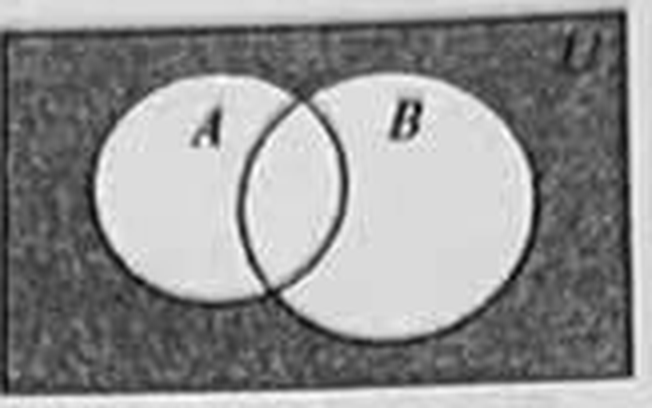
\includegraphics[width=0.30\textwidth]{figures/venn_AB_complement.png}
\end{center}

\ans{$\overline{A\cup B}$}

\ifanswer
\solbegin
\step{图中阴影部分在集合 $A$、$B$ 的外部，即在全集 $U$ 中但不属于 $A$、也不属于 $B$.}
\step{这正是 $A\cup B$ 在全集 $U$ 中的补集，故可表示为 $\overline{A\cup B}$（即 $\complement_U(A\cup B)$）.}
\solend

\fi

\item 设全集 $U=\R$，集合 $A=\{x\mid 2\leqslant x<5\}$，$B=\{x\mid 3<x<6\}$，则 $\overline{A}\cap B=$ \blankline[4.4em]（用区间表示）.

\ans{$[5,6)$}

\ifanswer
\solbegin
\step{在全集 $\R$ 中，$\overline{A}=(-\infty,2)\cup[5,+\infty)$.}
\step{又 $B=(3,6)$，取两集合的公共部分得 $\overline{A}\cap B=[5,6)$.}
\solend

\fi

\item 用反证法证明“$a,b\in\N$，$ab$ 可被 5 整除，那么 $a,b$ 中至少有一个能被 5 整除”时应假设 \blankline[4.4em].

\ans{$a,b$ 都不能被 5 整除}

\ifanswer
\solbegin
\step{反证法需假设结论的反面成立.}
\step{“$a,b$ 中至少有一个能被 5 整除”的反面是“$a,b$ 中没有一个能被 5 整除”，即 $a,b$ 都不能被 5 整除.}
\solend

\fi

\item 满足 $M\subseteq\{a_1,a_2,a_3,a_4,a_5\}$，且 $M\cap\{a_1,a_2,a_3\}=\{a_1,a_2\}$，则集合 $M$ 的个数是 \blankline[2.4em].

\ans{$4$}

\ifanswer
\solbegin
\step{由 $M\cap\{a_1,a_2,a_3\}=\{a_1,a_2\}$ 得 $a_1\in M$，$a_2\in M$，$a_3\notin M$.}
\step{又 $M\subseteq\{a_1,a_2,a_3,a_4,a_5\}$，所以 $a_4$、$a_5$ 可以属于 $M$，也可以不属于 $M$.}
\step{即 $M=\{a_1,a_2\}\cup S$，其中 $S\subseteq\{a_4,a_5\}$，共有 $2^2=4$ 个.}
\solend

\fi

\item 已知集合 $A=\{(x,y)\mid y=x^2\}$，$B=\left\{(x,y)\mid \dfrac{y-1}{x-1}=\dfrac{1}{2}\right\}$，则 $A\cap B=$ \blankline[5.2em].

\ans{$\left\{\left(-\dfrac{1}{2},\dfrac{1}{4}\right)\right\}$}

\ifanswer
\solbegin
\step{集合 $B$ 中的点满足 $y=\dfrac{1}{2}x+\dfrac{1}{2}$，且 $x\neq 1$.}
\step{代入 $y=x^2$ 得 $2x^2-x-1=0$，解得 $x=1$ 或 $x=-\dfrac{1}{2}$.}
\step{因为 $x\neq 1$，所以 $x=-\dfrac{1}{2}$，此时 $y=\dfrac{1}{4}$.}
\step{所以 $A\cap B=\left\{\left(-\dfrac{1}{2},\dfrac{1}{4}\right)\right\}$.}
\solend

\fi

\item 已知集合 $\{a,b,c\}=\{0,1,2\}$，且下列三个关系：①$a\neq 2$ ②$b=2$ ③$c\neq 0$ 有且只有一个正确，则 $100a+10b+c$ 等于 \blankline[2.4em].

\ans{$201$}

\ifanswer
\solbegin
\step{$a,b,c$ 是 $0,1,2$ 的一个排列，共 6 种情形，逐一检验三个关系的真假：}
\step{$(a,b,c)=(0,1,2)$：①真、②假、③真，两个正确，不合；$(0,2,1)$：三个都真，不合；}
\step{$(1,0,2)$：①真、②假、③真，两个正确，不合；$(1,2,0)$：①真、②真、③假，两个正确，不合；}
\step{$(2,0,1)$：①假、②假、③真，恰有一个正确，符合；$(2,1,0)$：三个都假，不合.}
\step{所以 $(a,b,c)=(2,0,1)$，$100a+10b+c=200+0+1=201$.}
\solend

\fi

\item “$x_1>3$ 且 $x_2>3$”是“$x_1+x_2>6$ 且 $x_1x_2>9$”的 \blankline[4.4em] 条件.（选填“充分非必要”，“必要非充分”，“充要”，“既非充分也非必要”）

\ans{充分非必要}

\ifanswer
\solbegin
\step{充分性：若 $x_1>3$ 且 $x_2>3$，则 $x_1+x_2>6$，且 $x_1x_2>9$，故充分性成立.}
\step{必要性：取 $x_1=2$、$x_2=5$，有 $x_1+x_2=7>6$、$x_1x_2=10>9$，但 $x_1>3$ 不成立，故必要性不成立.}
\step{所以应填“充分非必要”.}
\solend

\fi

% 注：第 11 题系 2010 年上海高考理科第 14 题的改写（原题要求选出 4 个子集，官方答案 36）。
%     原题官方解答明言「A、B 可以互换，即视为一种选法」，即**不计先后**计数；
%     按此口径本改写题的答案为 5。（原卷学生作答为 10，是把 A⊆B 与 B⊆A 重复计入。）
\item 在集合 $U=\{a,b,c,d\}$ 的子集中选出 2 个不同的子集，需同时满足以下两个条件：(1)$a,b$ 都要选出 (2)对选出的任意两个子集 $A$ 和 $B$，必有 $A\subseteq B$ 或 $B\subseteq A$，那么共有 \blankline[2.4em] 种不同的选法.

\ans{$5$}

\ifanswer
\solbegin
\step{由 (1) 知 $a,b$ 都要选出，即 $a,b$ 都属于所选的两个子集；由 (2) 知所选的两个子集必须可比.}
\step{含 $a,b$ 的子集只有 $\{a,b\}$、$\{a,b,c\}$、$\{a,b,d\}$、$\{a,b,c,d\}$ 共 4 个.}
\step{在这 4 个子集中取出两个不同的且可比的（一个包含另一个），只有下列 5 组：}
\step{$\{a,b\}\subset\{a,b,c\}$、$\{a,b\}\subset\{a,b,d\}$、$\{a,b\}\subset\{a,b,c,d\}$、$\{a,b,c\}\subset\{a,b,c,d\}$、$\{a,b,d\}\subset\{a,b,c,d\}$.}
\step{注意「选出 2 个子集」的选法\textbf{不计先后}：把这两个子集分别叫作 $A$、$B$ 只是给它们取个名字，$A\subseteq B$ 与 $B\subseteq A$ 说的是同一组子集，算同一种选法.}
\step{（本题由 2010 年上海高考理科第 14 题改写，原题要求选出 4 个子集，其官方答案 36 正是按「$A$、$B$ 可以互换，即视为一种选法」的不计先后口径计数.）}
\step{所以共有 5 种不同的选法.}
\solend

\fi

\end{enumerate}

\bigsec{二、选择题}

\begin{enumerate}
\setcounter{enumi}{11}

\item 已知 $M=(-\infty,\sqrt{3}]$，$a=\sqrt{3}$，则下列关系中正确的是（\quad）.

A. $a\subset M$\qquad B. $a\in M$\qquad C. $\{a\}\in M$\qquad D. $M\subset\{a\}$

\ans{B}

\ifanswer
\solbegin
\step{因为 $\sqrt{3}\leqslant\sqrt{3}$，所以 $a=\sqrt{3}\in M$，B 正确.}
\step{$a$ 是元素、$M$ 是集合，元素与集合之间用 $\in$ 表示，不能用 $\subset$，故 A、D 错误；}
\step{$\{a\}$ 是集合，集合与集合之间应是包含关系（且 $\{a\}\subseteq M$），不能用 $\in$，故 C 错误.}
\step{故选 B.}
\solend

\fi

% 注：原卷此处印作“已知集合{(x,y)|x^2+y^2≤3, x∈Z, y∈Z}”，集合未记作 A，
%     却设问“则 A 中的元素个数是”，显系漏排“A=”；本稿补上，其余照原卷。
\item 已知集合 $A=\{(x,y)\mid x^2+y^2\leqslant 3,\ x\in\Z,\ y\in\Z\}$，则 $A$ 中的元素个数是（\quad）.

A. $9$\qquad B. $8$\qquad C. $5$\qquad D. $4$

\ans{A}

\ifanswer
\solbegin
\step{逐一列举：$x=0$ 时 $y^2\leqslant 3$，$y=-1,0,1$，得 $(0,-1),(0,0),(0,1)$，共 3 个；}
\step{$x=\pm 1$ 时 $y^2\leqslant 2$，$y=-1,0,1$，各得 3 个，共 6 个（$x^2+y^2=2\leqslant 3$ 满足条件）；}
\step{$|x|\geqslant 2$ 时 $x^2\geqslant 4>3$，无解.}
\step{所以 $A$ 中元素个数为 $3+6=9$. 故选 A.}
\solend

\fi

\item 集合 $A=\{x\mid x=(2k-1)\pi,\ k\in\Z\}$ 与 $B=\{x\mid x=(4n\pm 1)\pi,\ n\in\Z\}$ 之间的关系是（\quad）.

A. $A\subset B$\qquad B. $B\subset A$\qquad C. $A=B$\qquad D. 不确定

\ans{C}

\ifanswer
\solbegin
\step{$A$ 由 $\pi$ 的一切奇数倍组成，即 $A=\{\cdots,-3\pi,-\pi,\pi,3\pi,\cdots\}$.}
\step{$B$ 中 $4n+1$ 与 $4n-1$ （$n\in\Z$）都是奇数，故 $B\subseteq A$；}
\step{反之，任一奇数除以 4 的余数只能是 1 或 3：形如 $4m+1$ 的奇数含于 $B$（取 $n=m$），形如 $4m+3=4(m+1)-1$ 的奇数也含于 $B$（取 $n=m+1$），所以 $A\subseteq B$.}
\step{于是 $A\subseteq B$ 且 $B\subseteq A$，即 $A=B$. 故选 C.}
\solend

\fi

\item 设 $T$ 是由正三角形 $P_1P_2P_3$ 边上及其内部的点构成的集合，点 $O$ 是 $\triangle P_1P_2P_3$ 的中心. 若集合 $S=\{P\mid P\in T,\ |PO|\leqslant|PO_i|,\ i=1,2,3\}$，（符号 $|AB|$ 表示平面上两点 $A,B$ 间的距离），则集合 $S$ 表示的平面区域是（\quad）.

A. 四边形区域；\qquad B. 三角形区域；\qquad C. 六边形区域；\qquad D. 五边形区域；

\ans{C}

\ifanswer
\solbegin
\step{$|PO|\leqslant|PO_i|$ 表示点 $P$ 到 $O$ 的距离不大于到顶点 $P_i$ 的距离，即 $P$ 落在线段 $OP_i$ 的垂直平分线靠 $O$ 的那一侧（含该线）.}
\step{对 $i=1,2,3$ 各有一条这样的直线，它们分别把三角形靠近 $P_1$、$P_2$、$P_3$ 的一个小角（三角形）截掉；}
\step{逐一直观验证可知这三条直线两两的交点都在三角形内部，三个角互不重叠，截去三个角后剩下的区域共有 6 条边.}
\step{所以集合 $S$ 表示的平面区域是六边形区域. 故选 C.}
\solend

\fi

\end{enumerate}

\bigsec{三、解答题}

\begin{enumerate}
\setcounter{enumi}{15}

\item（10 分，第 1 小问 5 分，第 2 小问 5 分）已知集合 $A=\{x\mid a\leqslant x\leqslant a+2\}$，集合 $B=\{x\mid x<-1\text{ 或 }x>5\}$，全集 $U=\R$.

\begin{enumerate}[label=(\arabic*)]
\item 若 $a=1$，求 $\overline{A}\cup B$；
\item 若 $A\subseteq B$，求实数 $a$ 的取值范围.
\end{enumerate}

\ans{（1）$(-\infty,1)\cup(3,+\infty)$；（2）$(-\infty,-3)\cup(5,+\infty)$}

\ifanswer
\solbegin
\stepm{(1)}{$a=1$ 时 $A=\{x\mid 1\leqslant x\leqslant 3\}=[1,3]$，则 $\overline{A}=(-\infty,1)\cup(3,+\infty)$.}
\step{又 $B=(-\infty,-1)\cup(5,+\infty)$，而 $B\subseteq\overline{A}$（因 $5>3$、$-1<1$），}
\step{所以 $\overline{A}\cup B=(-\infty,1)\cup(3,+\infty)$.}
\stepm{(2)}{因为 $a\leqslant a+2$，所以集合 $A=\{x\mid a\leqslant x\leqslant a+2\}$ 始终非空.}
\step{要使 $A\subseteq B$，只需 $A$ 与 $[-1,5]$ 没有公共点，即 $a+2<-1$ 或 $a>5$.}
\step{解得 $a<-3$ 或 $a>5$，所以实数 $a$ 的取值范围是 $(-\infty,-3)\cup(5,+\infty)$.}
\solend

\fi

\ansspace[10]

\item（10 分，第 1 小问 5 分，第 2 小问 5 分）已知 $A=\{x\mid x^2+x-2=0\}$，$B=\{x\mid x^2+ax+2a-4=0\}$.

\begin{enumerate}[label=(\arabic*)]
\item 若 $A=B$，求实数 $a$ 的值；
\item 若 $B\subseteq A$，求实数 $a$ 的值.
\end{enumerate}

\ans{（1）$a=1$；（2）$a=1$ 或 $a=4$}

\ifanswer
\solbegin
\stepm{(1)}{由 $x^2+x-2=0$ 解得 $x=1$ 或 $x=-2$，所以 $A=\{1,-2\}$.}
\step{由 $A=B$ 知 $1$、$-2$ 是方程 $x^2+ax+2a-4=0$ 的两根，由根与系数的关系得 $1+(-2)=-a$，所以 $a=1$；}
\step{此时 $2a-4=-2=1\times(-2)$，与两根之积相符，故 $a=1$.}
\stepm{(2)}{方程 $x^2+ax+2a-4=0$ 的判别式 $\Delta=a^2-4(2a-4)=(a-4)^2\geqslant 0$ 恒成立，所以集合 $B$ 不可能是空集.}
\step{由 $B\subseteq A$ 知 $B=\{1\}$ 或 $B=\{-2\}$ 或 $B=\{1,-2\}$.}
\step{若 $B=\{1\}$，则 $1$ 是二重根，$1+1=-a$ 且 $1\times 1=2a-4$，即 $a=-2$ 且 $a=\dfrac{5}{2}$，无解；}
\step{若 $B=\{-2\}$，则 $-2$ 是二重根，$(-2)+(-2)=-a$ 且 $(-2)\times(-2)=2a-4$，两式都给出 $a=4$，符合；}
\step{若 $B=\{1,-2\}$，则 $1+(-2)=-a$，得 $a=1$，此时 $2a-4=-2=1\times(-2)$，符合.}
\step{综上，$a=1$ 或 $a=4$.}
\solend

\fi

\ansspace[12]

\item（11 分，第 1 小问 3 分，第 2 小问 3 分，第 3 小问 5 分）已知非空数集 $S$ 满足：对任意给定的 $x,y\in S$（$x,y$ 可以相同），有 $x+y\in S$ 且 $x-y\in S$.

\begin{enumerate}[label=(\arabic*)]
\item 哪个数一定是 $S$ 中的元素?说明理由；
\item 若 $S$ 是有限集，求 $S$；
\item 若 $S$ 中最小的正数为 5，求 $S$.
\end{enumerate}

\ans{（1）$0$；（2）$S=\{0\}$；（3）$S=\{x\mid x=5a,\ a\in\Z\}$}

\ifanswer
\solbegin
\stepm{(1)}{$0$ 一定是 $S$ 中的元素. 理由：$S$ 非空，取 $x\in S$，在 $x-y\in S$ 中令 $y=x$（$x,y$ 可以相同），得 $x-x=0\in S$.}
\stepm{(2)}{若 $S$ 是有限集，则 $S=\{0\}$. 理由：取 $x\in S$ 且 $x\neq 0$，由 $x+y\in S$ 依次得 $2x=x+x\in S$，$3x=2x+x\in S$，$\cdots$，即 $kx\in S$（$k=1,2,3,\cdots$）；}
\step{这些数互不相同，与 $S$ 是有限集矛盾，所以 $S$ 中除 $0$ 外没有别的元素，即 $S=\{0\}$（此时 $0+0=0\in S$，$0-0=0\in S$，符合条件）.}
\stepm{(3)}{因为 $5\in S$，由 $x+y\in S$ 得 $5+5=10\in S$，$10+5=15\in S$，$\cdots$，故一切正整数倍的 $5$ 都在 $S$ 中；}
\step{又由 $x-y\in S$ 得 $5-5=0\in S$，$0-5=-5\in S$，$-5-5=-10\in S$，$\cdots$，故一切负整数倍的 $5$ 也都在 $S$ 中，即 $\{5a\mid a\in\Z\}\subseteq S$.}
\step{反之，任取 $s\in S$，由 $5\in S$ 及封闭性知 $s-5k\in S$（$k\in\Z$）；把 $s$ 写成 $s=5q+r$（$q\in\Z$，$0\leqslant r<5$），取 $k=q$ 得 $r=s-5q\in S$.}
\step{若 $r>0$，则 $S$ 中有比 $5$ 更小的正数 $r$，与“$S$ 中最小的正数为 5”矛盾，故只能 $r=0$，即 $s=5q$.}
\step{所以 $S=\{x\mid x=5a,\ a\in\Z\}$.}
\solend

\fi

\ansspace[12]

\end{enumerate}

\bigsec{附加题}

\begin{enumerate}
\setcounter{enumi}{18}

\item 已知集合 $A,B,C\subseteq\{1,2,3,\cdots,2024\}$，且 $A\subseteq B\subseteq C$，则有序集合组 $(A,B,C)$ 的个数是 \blankline[3.2em].

\ans{$4^{2024}$}

\ifanswer
\solbegin
\step{对 $U=\{1,2,\cdots,2024\}$ 中的每个元素，它与 $A,B,C$ 的关系只有四种可能：}
\step{在 $A,B,C$ 中都出现；不在 $A$ 中而在 $B,C$ 中出现；只在 $C$ 中出现；在三个集合中都不出现.}
\step{反过来，任取每个元素的一种归属方式，都恰好得到一个满足 $A\subseteq B\subseteq C$ 的有序集合组，故不同的组与不同的归属方式一一对应.}
\step{所以共有 $4\times 4\times\cdots\times 4=4^{2024}$ 个有序集合组.}
\solend

\fi

\item 已知集合 $M=\{1,2,\cdots,10\}$，对它的非空子集 $A$，将 $A$ 中的每个元素 $k$ 都乘以 $(-1)^k$ 再求和，如 $A=\{2,3,6\}$，可求得和为 $(-1)^2\times 2+(-1)^3\times 3+(-1)^6\times 6=5$. 试对 $M$ 的所有非空子集，求这些和的总和 \blankline[3.2em].

\ans{$2560$}

\ifanswer
\solbegin
\step{元素 $k$（$k=1,2,\cdots,10$）出现在 $M$ 的 $2^{9}$ 个非空子集中（其余 9 个元素任取）.}
\step{所以在所有非空子集的和中，$k$ 贡献的总量为 $2^{9}\times(-1)^k\cdot k=512\times(-1)^kk$.}
\step{于是这些和的总和为 $512\displaystyle\sum_{k=1}^{10}(-1)^kk=512\times(-1+2-3+4-5+6-7+8-9+10)=512\times 5=2560$.}
\solend

\fi

\item 设 $a_1,a_2,a_3,a_4$ 是 4 个有理数，使得 $\{a_ia_j\mid 1\leqslant i<j\leqslant 4\}=\left\{-24,-2,-\dfrac{3}{2},-\dfrac{1}{8},1,3\right\}$. 求 $a_1+a_2+a_3+a_4=$ \blankline[3.2em].

\ans{$\pm\dfrac{9}{4}$（两组解，和分别为 $-\dfrac{9}{4}$ 与 $\dfrac{9}{4}$）}

\ifanswer
\solbegin
\step{六个乘积中有 4 个负数、2 个正数. 设 4 个数中正数有 $p$ 个、负数有 $q$ 个（$p+q=4$），则异号的两数相乘得负数，其个数为 $pq$；由 $pq=4$ 得 $p=q=2$，即恰有 2 个正数、2 个负数.}
\step{把 4 个数的绝对值记作 $w,x,y,z>0$，则六个两两乘积的绝对值为 $24,2,\dfrac{3}{2},\dfrac{1}{8},1,3$；其中 $1$ 与 $3$ 来自两对同号的数，$24,2,\dfrac{3}{2},\dfrac{1}{8}$ 来自四对异号的数.}
\step{由 $(a_1a_2a_3a_4)^3=(-24)\times(-2)\times\left(-\dfrac{3}{2}\right)\times\left(-\dfrac{1}{8}\right)\times 1\times 3=27$ 得 $a_1a_2a_3a_4=3$，即去符号后 $wxyz=3$.}
\step{逐一检验可知 $w,x,y,z$ 只能是 $\left\{4,\dfrac{1}{4},6,\dfrac{1}{2}\right\}$：其中 $4\times\dfrac{1}{4}=1$、$6\times\dfrac{1}{2}=3$ 为同号两对的乘积，$4\times 6=24$、$4\times\dfrac{1}{2}=2$、$\dfrac{1}{4}\times 6=\dfrac{3}{2}$、$\dfrac{1}{4}\times\dfrac{1}{2}=\dfrac{1}{8}$ 为异号四对的乘积.}
\step{于是 $\left\{4,\dfrac{1}{4}\right\}$ 中的两个数同号、$\left\{6,\dfrac{1}{2}\right\}$ 中的两个数同号，且这两组异号，得两组解：}
\step{$4,\ \dfrac{1}{4},\ -6,\ -\dfrac{1}{2}$，和为 $-\dfrac{9}{4}$；\quad 或 \quad $6,\ \dfrac{1}{2},\ -4,\ -\dfrac{1}{4}$，和为 $\dfrac{9}{4}$.}
\step{两组解的六个乘积都恰为 $-24,-2,-\dfrac{3}{2},-\dfrac{1}{8},1,3$，与原卷所给集合相同.}
\step{所以 $a_1+a_2+a_3+a_4=\pm\dfrac{9}{4}$.}
\solend

\fi

\end{enumerate}

\end{document}
"
% 紧凑版：xelatex "\def\iscompact{1}% 高一16_大同中学_第二周周末练习1.tex —— 高一上数学「第二周周末练习1」（试卷版/答案版）
% 试卷版：xelatex 高一16_大同中学_第二周周末练习1.tex
% 答案版：xelatex "\def\isanswer{1}% 高一16_大同中学_第二周周末练习1.tex —— 高一上数学「第二周周末练习1」（试卷版/答案版）
% 试卷版：xelatex 高一16_大同中学_第二周周末练习1.tex
% 答案版：xelatex "\def\isanswer{1}\input{高一16_大同中学_第二周周末练习1.tex}"
% 紧凑版：xelatex "\def\iscompact{1}\input{高一16_大同中学_第二周周末练习1.tex}"
%
% 原始材料为学生作业的手机翻拍照片（卷面为学生本人的**手写作答**，未见教师批改痕迹）。
% 试题文字照原卷录入；答案版给出的是**经核验的正确解答与解析**，与原卷手写答案的差异见 README。
%
% 与原卷的两处排版差异（均已在 README「说明」中交代）：
%   ① 原卷未印分节标题与分值，本稿按题型补「一、填空题 / 二、选择题 / 三、解答题」三节
%      （「附加题」原卷有印）；
%   ② 第 13 题原卷印作「已知集合{(x,y)|…}」，集合未记作 A 却被设问为「A 中的元素个数」，
%      显系漏排「A=」，本稿补上。

% 本篇的正文与家长拍照卷 `高一b_大同中学_第二周周末练习1（补）` **完全相同**——同一份作业，
% 试卷版/答案版也都是同一份源码编译而来；`高一b` 的 4 张原图另存于
% `原图/高一b_大同中学_第二周周末练习1（补）/`，本卷 `原图/` 下是同一组照片的副本。
% 经核对，这份作业就是公众号「魔都数学加油站」连载「27学年高一16——2026-2027年上海市大同中学
% 高一上周末作业2.1」的那一份：**题号与题干逐题一致**，只是公众号版略去了填空第 1、2 题，
% 故拍照卷反而是更完整的版本（对照关系见 README「与公众号连载号的对照表」）。
%
% 本卷的编号与连载号对齐（高一16），卷面标题因此**不带**「（补）」；标题里的「大同中学」为**本稿所加**
% （原卷标题只有作业名，校名只印在页眉「上海市大同…」）。带「（补）」的 `高一b` 保留为
% 拍照原件的转录本，两者内容一字不差。
%
% 一处与公众号讲评版的差异需留意：本卷第 11 题的答案按 2010 年上海高考理科第 14 题官方解答
% 「A、B 可以互换，即视为一种选法」的不计先后口径取 5，而公众号讲评版把它按有先后的 32 计数
% （该题学生原作答为 10）。取舍理由见该题下的 `%` 注。
\documentclass[a4paper,11pt]{article}
\usepackage{common}

\begin{document}

\examtitlest[3]{2026--2027 学年度大同中学高一上数学第二周周末练习1}{集合与常用逻辑用语}

\bigsec{一、填空题}

\begin{enumerate}

\item 用列举法表示集合 $\{x\mid -2<x\leqslant 2,\ x\in\Z\}=$ \blankline[2.4em].

\ans{$\{-1,0,1,2\}$}

\ifanswer
\solbegin
\step{集合中的元素是满足 $-2<x\leqslant 2$ 的整数，即 $-1$、$0$、$1$、$2$.}
\step{所以用列举法表示为 $\{-1,0,1,2\}$.}
\solend

\fi

\item 设集合 $A=\{1,a\}$，$B=\{1,a^2\}$，若 $A=B$，则实数 $a$ 的值为 \blankline[2.4em].

\ans{$a=0$}

\ifanswer
\solbegin
\step{由 $A=B$ 得 $a^2=a$，解得 $a=0$ 或 $a=1$.}
\step{当 $a=1$ 时，$A=\{1,1\}$，不符合集合元素的互异性，舍去；}
\step{当 $a=0$ 时，$A=\{1,0\}$，$B=\{1,0\}$，两集合相等，符合条件.}
\step{所以 $a=0$.}
\solend

\fi

\item 已知集合 $A=\{0,2,3,4,5\}$，$B=\{2,3,5,7\}$，$C=\{2,3,6\}$，则 $(A\cap B)\cup C=$ \blankline[4.4em].

\ans{$\{2,3,5,6\}$}

\ifanswer
\solbegin
\step{$A\cap B=\{0,2,3,4,5\}\cap\{2,3,5,7\}=\{2,3,5\}$.}
\step{所以 $(A\cap B)\cup C=\{2,3,5\}\cup\{2,3,6\}=\{2,3,5,6\}$.}
\solend

\fi

\item 设全集为 $U$，用集合 $A,B$ 的交、并或补集符号表示图中的阴影部分是 \blankline[4.4em].

\begin{center}
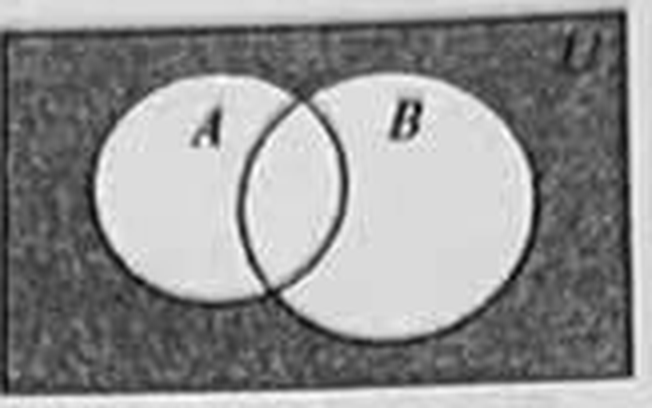
\includegraphics[width=0.30\textwidth]{figures/venn_AB_complement.png}
\end{center}

\ans{$\overline{A\cup B}$}

\ifanswer
\solbegin
\step{图中阴影部分在集合 $A$、$B$ 的外部，即在全集 $U$ 中但不属于 $A$、也不属于 $B$.}
\step{这正是 $A\cup B$ 在全集 $U$ 中的补集，故可表示为 $\overline{A\cup B}$（即 $\complement_U(A\cup B)$）.}
\solend

\fi

\item 设全集 $U=\R$，集合 $A=\{x\mid 2\leqslant x<5\}$，$B=\{x\mid 3<x<6\}$，则 $\overline{A}\cap B=$ \blankline[4.4em]（用区间表示）.

\ans{$[5,6)$}

\ifanswer
\solbegin
\step{在全集 $\R$ 中，$\overline{A}=(-\infty,2)\cup[5,+\infty)$.}
\step{又 $B=(3,6)$，取两集合的公共部分得 $\overline{A}\cap B=[5,6)$.}
\solend

\fi

\item 用反证法证明“$a,b\in\N$，$ab$ 可被 5 整除，那么 $a,b$ 中至少有一个能被 5 整除”时应假设 \blankline[4.4em].

\ans{$a,b$ 都不能被 5 整除}

\ifanswer
\solbegin
\step{反证法需假设结论的反面成立.}
\step{“$a,b$ 中至少有一个能被 5 整除”的反面是“$a,b$ 中没有一个能被 5 整除”，即 $a,b$ 都不能被 5 整除.}
\solend

\fi

\item 满足 $M\subseteq\{a_1,a_2,a_3,a_4,a_5\}$，且 $M\cap\{a_1,a_2,a_3\}=\{a_1,a_2\}$，则集合 $M$ 的个数是 \blankline[2.4em].

\ans{$4$}

\ifanswer
\solbegin
\step{由 $M\cap\{a_1,a_2,a_3\}=\{a_1,a_2\}$ 得 $a_1\in M$，$a_2\in M$，$a_3\notin M$.}
\step{又 $M\subseteq\{a_1,a_2,a_3,a_4,a_5\}$，所以 $a_4$、$a_5$ 可以属于 $M$，也可以不属于 $M$.}
\step{即 $M=\{a_1,a_2\}\cup S$，其中 $S\subseteq\{a_4,a_5\}$，共有 $2^2=4$ 个.}
\solend

\fi

\item 已知集合 $A=\{(x,y)\mid y=x^2\}$，$B=\left\{(x,y)\mid \dfrac{y-1}{x-1}=\dfrac{1}{2}\right\}$，则 $A\cap B=$ \blankline[5.2em].

\ans{$\left\{\left(-\dfrac{1}{2},\dfrac{1}{4}\right)\right\}$}

\ifanswer
\solbegin
\step{集合 $B$ 中的点满足 $y=\dfrac{1}{2}x+\dfrac{1}{2}$，且 $x\neq 1$.}
\step{代入 $y=x^2$ 得 $2x^2-x-1=0$，解得 $x=1$ 或 $x=-\dfrac{1}{2}$.}
\step{因为 $x\neq 1$，所以 $x=-\dfrac{1}{2}$，此时 $y=\dfrac{1}{4}$.}
\step{所以 $A\cap B=\left\{\left(-\dfrac{1}{2},\dfrac{1}{4}\right)\right\}$.}
\solend

\fi

\item 已知集合 $\{a,b,c\}=\{0,1,2\}$，且下列三个关系：①$a\neq 2$ ②$b=2$ ③$c\neq 0$ 有且只有一个正确，则 $100a+10b+c$ 等于 \blankline[2.4em].

\ans{$201$}

\ifanswer
\solbegin
\step{$a,b,c$ 是 $0,1,2$ 的一个排列，共 6 种情形，逐一检验三个关系的真假：}
\step{$(a,b,c)=(0,1,2)$：①真、②假、③真，两个正确，不合；$(0,2,1)$：三个都真，不合；}
\step{$(1,0,2)$：①真、②假、③真，两个正确，不合；$(1,2,0)$：①真、②真、③假，两个正确，不合；}
\step{$(2,0,1)$：①假、②假、③真，恰有一个正确，符合；$(2,1,0)$：三个都假，不合.}
\step{所以 $(a,b,c)=(2,0,1)$，$100a+10b+c=200+0+1=201$.}
\solend

\fi

\item “$x_1>3$ 且 $x_2>3$”是“$x_1+x_2>6$ 且 $x_1x_2>9$”的 \blankline[4.4em] 条件.（选填“充分非必要”，“必要非充分”，“充要”，“既非充分也非必要”）

\ans{充分非必要}

\ifanswer
\solbegin
\step{充分性：若 $x_1>3$ 且 $x_2>3$，则 $x_1+x_2>6$，且 $x_1x_2>9$，故充分性成立.}
\step{必要性：取 $x_1=2$、$x_2=5$，有 $x_1+x_2=7>6$、$x_1x_2=10>9$，但 $x_1>3$ 不成立，故必要性不成立.}
\step{所以应填“充分非必要”.}
\solend

\fi

% 注：第 11 题系 2010 年上海高考理科第 14 题的改写（原题要求选出 4 个子集，官方答案 36）。
%     原题官方解答明言「A、B 可以互换，即视为一种选法」，即**不计先后**计数；
%     按此口径本改写题的答案为 5。（原卷学生作答为 10，是把 A⊆B 与 B⊆A 重复计入。）
\item 在集合 $U=\{a,b,c,d\}$ 的子集中选出 2 个不同的子集，需同时满足以下两个条件：(1)$a,b$ 都要选出 (2)对选出的任意两个子集 $A$ 和 $B$，必有 $A\subseteq B$ 或 $B\subseteq A$，那么共有 \blankline[2.4em] 种不同的选法.

\ans{$5$}

\ifanswer
\solbegin
\step{由 (1) 知 $a,b$ 都要选出，即 $a,b$ 都属于所选的两个子集；由 (2) 知所选的两个子集必须可比.}
\step{含 $a,b$ 的子集只有 $\{a,b\}$、$\{a,b,c\}$、$\{a,b,d\}$、$\{a,b,c,d\}$ 共 4 个.}
\step{在这 4 个子集中取出两个不同的且可比的（一个包含另一个），只有下列 5 组：}
\step{$\{a,b\}\subset\{a,b,c\}$、$\{a,b\}\subset\{a,b,d\}$、$\{a,b\}\subset\{a,b,c,d\}$、$\{a,b,c\}\subset\{a,b,c,d\}$、$\{a,b,d\}\subset\{a,b,c,d\}$.}
\step{注意「选出 2 个子集」的选法\textbf{不计先后}：把这两个子集分别叫作 $A$、$B$ 只是给它们取个名字，$A\subseteq B$ 与 $B\subseteq A$ 说的是同一组子集，算同一种选法.}
\step{（本题由 2010 年上海高考理科第 14 题改写，原题要求选出 4 个子集，其官方答案 36 正是按「$A$、$B$ 可以互换，即视为一种选法」的不计先后口径计数.）}
\step{所以共有 5 种不同的选法.}
\solend

\fi

\end{enumerate}

\bigsec{二、选择题}

\begin{enumerate}
\setcounter{enumi}{11}

\item 已知 $M=(-\infty,\sqrt{3}]$，$a=\sqrt{3}$，则下列关系中正确的是（\quad）.

A. $a\subset M$\qquad B. $a\in M$\qquad C. $\{a\}\in M$\qquad D. $M\subset\{a\}$

\ans{B}

\ifanswer
\solbegin
\step{因为 $\sqrt{3}\leqslant\sqrt{3}$，所以 $a=\sqrt{3}\in M$，B 正确.}
\step{$a$ 是元素、$M$ 是集合，元素与集合之间用 $\in$ 表示，不能用 $\subset$，故 A、D 错误；}
\step{$\{a\}$ 是集合，集合与集合之间应是包含关系（且 $\{a\}\subseteq M$），不能用 $\in$，故 C 错误.}
\step{故选 B.}
\solend

\fi

% 注：原卷此处印作“已知集合{(x,y)|x^2+y^2≤3, x∈Z, y∈Z}”，集合未记作 A，
%     却设问“则 A 中的元素个数是”，显系漏排“A=”；本稿补上，其余照原卷。
\item 已知集合 $A=\{(x,y)\mid x^2+y^2\leqslant 3,\ x\in\Z,\ y\in\Z\}$，则 $A$ 中的元素个数是（\quad）.

A. $9$\qquad B. $8$\qquad C. $5$\qquad D. $4$

\ans{A}

\ifanswer
\solbegin
\step{逐一列举：$x=0$ 时 $y^2\leqslant 3$，$y=-1,0,1$，得 $(0,-1),(0,0),(0,1)$，共 3 个；}
\step{$x=\pm 1$ 时 $y^2\leqslant 2$，$y=-1,0,1$，各得 3 个，共 6 个（$x^2+y^2=2\leqslant 3$ 满足条件）；}
\step{$|x|\geqslant 2$ 时 $x^2\geqslant 4>3$，无解.}
\step{所以 $A$ 中元素个数为 $3+6=9$. 故选 A.}
\solend

\fi

\item 集合 $A=\{x\mid x=(2k-1)\pi,\ k\in\Z\}$ 与 $B=\{x\mid x=(4n\pm 1)\pi,\ n\in\Z\}$ 之间的关系是（\quad）.

A. $A\subset B$\qquad B. $B\subset A$\qquad C. $A=B$\qquad D. 不确定

\ans{C}

\ifanswer
\solbegin
\step{$A$ 由 $\pi$ 的一切奇数倍组成，即 $A=\{\cdots,-3\pi,-\pi,\pi,3\pi,\cdots\}$.}
\step{$B$ 中 $4n+1$ 与 $4n-1$ （$n\in\Z$）都是奇数，故 $B\subseteq A$；}
\step{反之，任一奇数除以 4 的余数只能是 1 或 3：形如 $4m+1$ 的奇数含于 $B$（取 $n=m$），形如 $4m+3=4(m+1)-1$ 的奇数也含于 $B$（取 $n=m+1$），所以 $A\subseteq B$.}
\step{于是 $A\subseteq B$ 且 $B\subseteq A$，即 $A=B$. 故选 C.}
\solend

\fi

\item 设 $T$ 是由正三角形 $P_1P_2P_3$ 边上及其内部的点构成的集合，点 $O$ 是 $\triangle P_1P_2P_3$ 的中心. 若集合 $S=\{P\mid P\in T,\ |PO|\leqslant|PO_i|,\ i=1,2,3\}$，（符号 $|AB|$ 表示平面上两点 $A,B$ 间的距离），则集合 $S$ 表示的平面区域是（\quad）.

A. 四边形区域；\qquad B. 三角形区域；\qquad C. 六边形区域；\qquad D. 五边形区域；

\ans{C}

\ifanswer
\solbegin
\step{$|PO|\leqslant|PO_i|$ 表示点 $P$ 到 $O$ 的距离不大于到顶点 $P_i$ 的距离，即 $P$ 落在线段 $OP_i$ 的垂直平分线靠 $O$ 的那一侧（含该线）.}
\step{对 $i=1,2,3$ 各有一条这样的直线，它们分别把三角形靠近 $P_1$、$P_2$、$P_3$ 的一个小角（三角形）截掉；}
\step{逐一直观验证可知这三条直线两两的交点都在三角形内部，三个角互不重叠，截去三个角后剩下的区域共有 6 条边.}
\step{所以集合 $S$ 表示的平面区域是六边形区域. 故选 C.}
\solend

\fi

\end{enumerate}

\bigsec{三、解答题}

\begin{enumerate}
\setcounter{enumi}{15}

\item（10 分，第 1 小问 5 分，第 2 小问 5 分）已知集合 $A=\{x\mid a\leqslant x\leqslant a+2\}$，集合 $B=\{x\mid x<-1\text{ 或 }x>5\}$，全集 $U=\R$.

\begin{enumerate}[label=(\arabic*)]
\item 若 $a=1$，求 $\overline{A}\cup B$；
\item 若 $A\subseteq B$，求实数 $a$ 的取值范围.
\end{enumerate}

\ans{（1）$(-\infty,1)\cup(3,+\infty)$；（2）$(-\infty,-3)\cup(5,+\infty)$}

\ifanswer
\solbegin
\stepm{(1)}{$a=1$ 时 $A=\{x\mid 1\leqslant x\leqslant 3\}=[1,3]$，则 $\overline{A}=(-\infty,1)\cup(3,+\infty)$.}
\step{又 $B=(-\infty,-1)\cup(5,+\infty)$，而 $B\subseteq\overline{A}$（因 $5>3$、$-1<1$），}
\step{所以 $\overline{A}\cup B=(-\infty,1)\cup(3,+\infty)$.}
\stepm{(2)}{因为 $a\leqslant a+2$，所以集合 $A=\{x\mid a\leqslant x\leqslant a+2\}$ 始终非空.}
\step{要使 $A\subseteq B$，只需 $A$ 与 $[-1,5]$ 没有公共点，即 $a+2<-1$ 或 $a>5$.}
\step{解得 $a<-3$ 或 $a>5$，所以实数 $a$ 的取值范围是 $(-\infty,-3)\cup(5,+\infty)$.}
\solend

\fi

\ansspace[10]

\item（10 分，第 1 小问 5 分，第 2 小问 5 分）已知 $A=\{x\mid x^2+x-2=0\}$，$B=\{x\mid x^2+ax+2a-4=0\}$.

\begin{enumerate}[label=(\arabic*)]
\item 若 $A=B$，求实数 $a$ 的值；
\item 若 $B\subseteq A$，求实数 $a$ 的值.
\end{enumerate}

\ans{（1）$a=1$；（2）$a=1$ 或 $a=4$}

\ifanswer
\solbegin
\stepm{(1)}{由 $x^2+x-2=0$ 解得 $x=1$ 或 $x=-2$，所以 $A=\{1,-2\}$.}
\step{由 $A=B$ 知 $1$、$-2$ 是方程 $x^2+ax+2a-4=0$ 的两根，由根与系数的关系得 $1+(-2)=-a$，所以 $a=1$；}
\step{此时 $2a-4=-2=1\times(-2)$，与两根之积相符，故 $a=1$.}
\stepm{(2)}{方程 $x^2+ax+2a-4=0$ 的判别式 $\Delta=a^2-4(2a-4)=(a-4)^2\geqslant 0$ 恒成立，所以集合 $B$ 不可能是空集.}
\step{由 $B\subseteq A$ 知 $B=\{1\}$ 或 $B=\{-2\}$ 或 $B=\{1,-2\}$.}
\step{若 $B=\{1\}$，则 $1$ 是二重根，$1+1=-a$ 且 $1\times 1=2a-4$，即 $a=-2$ 且 $a=\dfrac{5}{2}$，无解；}
\step{若 $B=\{-2\}$，则 $-2$ 是二重根，$(-2)+(-2)=-a$ 且 $(-2)\times(-2)=2a-4$，两式都给出 $a=4$，符合；}
\step{若 $B=\{1,-2\}$，则 $1+(-2)=-a$，得 $a=1$，此时 $2a-4=-2=1\times(-2)$，符合.}
\step{综上，$a=1$ 或 $a=4$.}
\solend

\fi

\ansspace[12]

\item（11 分，第 1 小问 3 分，第 2 小问 3 分，第 3 小问 5 分）已知非空数集 $S$ 满足：对任意给定的 $x,y\in S$（$x,y$ 可以相同），有 $x+y\in S$ 且 $x-y\in S$.

\begin{enumerate}[label=(\arabic*)]
\item 哪个数一定是 $S$ 中的元素?说明理由；
\item 若 $S$ 是有限集，求 $S$；
\item 若 $S$ 中最小的正数为 5，求 $S$.
\end{enumerate}

\ans{（1）$0$；（2）$S=\{0\}$；（3）$S=\{x\mid x=5a,\ a\in\Z\}$}

\ifanswer
\solbegin
\stepm{(1)}{$0$ 一定是 $S$ 中的元素. 理由：$S$ 非空，取 $x\in S$，在 $x-y\in S$ 中令 $y=x$（$x,y$ 可以相同），得 $x-x=0\in S$.}
\stepm{(2)}{若 $S$ 是有限集，则 $S=\{0\}$. 理由：取 $x\in S$ 且 $x\neq 0$，由 $x+y\in S$ 依次得 $2x=x+x\in S$，$3x=2x+x\in S$，$\cdots$，即 $kx\in S$（$k=1,2,3,\cdots$）；}
\step{这些数互不相同，与 $S$ 是有限集矛盾，所以 $S$ 中除 $0$ 外没有别的元素，即 $S=\{0\}$（此时 $0+0=0\in S$，$0-0=0\in S$，符合条件）.}
\stepm{(3)}{因为 $5\in S$，由 $x+y\in S$ 得 $5+5=10\in S$，$10+5=15\in S$，$\cdots$，故一切正整数倍的 $5$ 都在 $S$ 中；}
\step{又由 $x-y\in S$ 得 $5-5=0\in S$，$0-5=-5\in S$，$-5-5=-10\in S$，$\cdots$，故一切负整数倍的 $5$ 也都在 $S$ 中，即 $\{5a\mid a\in\Z\}\subseteq S$.}
\step{反之，任取 $s\in S$，由 $5\in S$ 及封闭性知 $s-5k\in S$（$k\in\Z$）；把 $s$ 写成 $s=5q+r$（$q\in\Z$，$0\leqslant r<5$），取 $k=q$ 得 $r=s-5q\in S$.}
\step{若 $r>0$，则 $S$ 中有比 $5$ 更小的正数 $r$，与“$S$ 中最小的正数为 5”矛盾，故只能 $r=0$，即 $s=5q$.}
\step{所以 $S=\{x\mid x=5a,\ a\in\Z\}$.}
\solend

\fi

\ansspace[12]

\end{enumerate}

\bigsec{附加题}

\begin{enumerate}
\setcounter{enumi}{18}

\item 已知集合 $A,B,C\subseteq\{1,2,3,\cdots,2024\}$，且 $A\subseteq B\subseteq C$，则有序集合组 $(A,B,C)$ 的个数是 \blankline[3.2em].

\ans{$4^{2024}$}

\ifanswer
\solbegin
\step{对 $U=\{1,2,\cdots,2024\}$ 中的每个元素，它与 $A,B,C$ 的关系只有四种可能：}
\step{在 $A,B,C$ 中都出现；不在 $A$ 中而在 $B,C$ 中出现；只在 $C$ 中出现；在三个集合中都不出现.}
\step{反过来，任取每个元素的一种归属方式，都恰好得到一个满足 $A\subseteq B\subseteq C$ 的有序集合组，故不同的组与不同的归属方式一一对应.}
\step{所以共有 $4\times 4\times\cdots\times 4=4^{2024}$ 个有序集合组.}
\solend

\fi

\item 已知集合 $M=\{1,2,\cdots,10\}$，对它的非空子集 $A$，将 $A$ 中的每个元素 $k$ 都乘以 $(-1)^k$ 再求和，如 $A=\{2,3,6\}$，可求得和为 $(-1)^2\times 2+(-1)^3\times 3+(-1)^6\times 6=5$. 试对 $M$ 的所有非空子集，求这些和的总和 \blankline[3.2em].

\ans{$2560$}

\ifanswer
\solbegin
\step{元素 $k$（$k=1,2,\cdots,10$）出现在 $M$ 的 $2^{9}$ 个非空子集中（其余 9 个元素任取）.}
\step{所以在所有非空子集的和中，$k$ 贡献的总量为 $2^{9}\times(-1)^k\cdot k=512\times(-1)^kk$.}
\step{于是这些和的总和为 $512\displaystyle\sum_{k=1}^{10}(-1)^kk=512\times(-1+2-3+4-5+6-7+8-9+10)=512\times 5=2560$.}
\solend

\fi

\item 设 $a_1,a_2,a_3,a_4$ 是 4 个有理数，使得 $\{a_ia_j\mid 1\leqslant i<j\leqslant 4\}=\left\{-24,-2,-\dfrac{3}{2},-\dfrac{1}{8},1,3\right\}$. 求 $a_1+a_2+a_3+a_4=$ \blankline[3.2em].

\ans{$\pm\dfrac{9}{4}$（两组解，和分别为 $-\dfrac{9}{4}$ 与 $\dfrac{9}{4}$）}

\ifanswer
\solbegin
\step{六个乘积中有 4 个负数、2 个正数. 设 4 个数中正数有 $p$ 个、负数有 $q$ 个（$p+q=4$），则异号的两数相乘得负数，其个数为 $pq$；由 $pq=4$ 得 $p=q=2$，即恰有 2 个正数、2 个负数.}
\step{把 4 个数的绝对值记作 $w,x,y,z>0$，则六个两两乘积的绝对值为 $24,2,\dfrac{3}{2},\dfrac{1}{8},1,3$；其中 $1$ 与 $3$ 来自两对同号的数，$24,2,\dfrac{3}{2},\dfrac{1}{8}$ 来自四对异号的数.}
\step{由 $(a_1a_2a_3a_4)^3=(-24)\times(-2)\times\left(-\dfrac{3}{2}\right)\times\left(-\dfrac{1}{8}\right)\times 1\times 3=27$ 得 $a_1a_2a_3a_4=3$，即去符号后 $wxyz=3$.}
\step{逐一检验可知 $w,x,y,z$ 只能是 $\left\{4,\dfrac{1}{4},6,\dfrac{1}{2}\right\}$：其中 $4\times\dfrac{1}{4}=1$、$6\times\dfrac{1}{2}=3$ 为同号两对的乘积，$4\times 6=24$、$4\times\dfrac{1}{2}=2$、$\dfrac{1}{4}\times 6=\dfrac{3}{2}$、$\dfrac{1}{4}\times\dfrac{1}{2}=\dfrac{1}{8}$ 为异号四对的乘积.}
\step{于是 $\left\{4,\dfrac{1}{4}\right\}$ 中的两个数同号、$\left\{6,\dfrac{1}{2}\right\}$ 中的两个数同号，且这两组异号，得两组解：}
\step{$4,\ \dfrac{1}{4},\ -6,\ -\dfrac{1}{2}$，和为 $-\dfrac{9}{4}$；\quad 或 \quad $6,\ \dfrac{1}{2},\ -4,\ -\dfrac{1}{4}$，和为 $\dfrac{9}{4}$.}
\step{两组解的六个乘积都恰为 $-24,-2,-\dfrac{3}{2},-\dfrac{1}{8},1,3$，与原卷所给集合相同.}
\step{所以 $a_1+a_2+a_3+a_4=\pm\dfrac{9}{4}$.}
\solend

\fi

\end{enumerate}

\end{document}
"
% 紧凑版：xelatex "\def\iscompact{1}% 高一16_大同中学_第二周周末练习1.tex —— 高一上数学「第二周周末练习1」（试卷版/答案版）
% 试卷版：xelatex 高一16_大同中学_第二周周末练习1.tex
% 答案版：xelatex "\def\isanswer{1}\input{高一16_大同中学_第二周周末练习1.tex}"
% 紧凑版：xelatex "\def\iscompact{1}\input{高一16_大同中学_第二周周末练习1.tex}"
%
% 原始材料为学生作业的手机翻拍照片（卷面为学生本人的**手写作答**，未见教师批改痕迹）。
% 试题文字照原卷录入；答案版给出的是**经核验的正确解答与解析**，与原卷手写答案的差异见 README。
%
% 与原卷的两处排版差异（均已在 README「说明」中交代）：
%   ① 原卷未印分节标题与分值，本稿按题型补「一、填空题 / 二、选择题 / 三、解答题」三节
%      （「附加题」原卷有印）；
%   ② 第 13 题原卷印作「已知集合{(x,y)|…}」，集合未记作 A 却被设问为「A 中的元素个数」，
%      显系漏排「A=」，本稿补上。

% 本篇的正文与家长拍照卷 `高一b_大同中学_第二周周末练习1（补）` **完全相同**——同一份作业，
% 试卷版/答案版也都是同一份源码编译而来；`高一b` 的 4 张原图另存于
% `原图/高一b_大同中学_第二周周末练习1（补）/`，本卷 `原图/` 下是同一组照片的副本。
% 经核对，这份作业就是公众号「魔都数学加油站」连载「27学年高一16——2026-2027年上海市大同中学
% 高一上周末作业2.1」的那一份：**题号与题干逐题一致**，只是公众号版略去了填空第 1、2 题，
% 故拍照卷反而是更完整的版本（对照关系见 README「与公众号连载号的对照表」）。
%
% 本卷的编号与连载号对齐（高一16），卷面标题因此**不带**「（补）」；标题里的「大同中学」为**本稿所加**
% （原卷标题只有作业名，校名只印在页眉「上海市大同…」）。带「（补）」的 `高一b` 保留为
% 拍照原件的转录本，两者内容一字不差。
%
% 一处与公众号讲评版的差异需留意：本卷第 11 题的答案按 2010 年上海高考理科第 14 题官方解答
% 「A、B 可以互换，即视为一种选法」的不计先后口径取 5，而公众号讲评版把它按有先后的 32 计数
% （该题学生原作答为 10）。取舍理由见该题下的 `%` 注。
\documentclass[a4paper,11pt]{article}
\usepackage{common}

\begin{document}

\examtitlest[3]{2026--2027 学年度大同中学高一上数学第二周周末练习1}{集合与常用逻辑用语}

\bigsec{一、填空题}

\begin{enumerate}

\item 用列举法表示集合 $\{x\mid -2<x\leqslant 2,\ x\in\Z\}=$ \blankline[2.4em].

\ans{$\{-1,0,1,2\}$}

\ifanswer
\solbegin
\step{集合中的元素是满足 $-2<x\leqslant 2$ 的整数，即 $-1$、$0$、$1$、$2$.}
\step{所以用列举法表示为 $\{-1,0,1,2\}$.}
\solend

\fi

\item 设集合 $A=\{1,a\}$，$B=\{1,a^2\}$，若 $A=B$，则实数 $a$ 的值为 \blankline[2.4em].

\ans{$a=0$}

\ifanswer
\solbegin
\step{由 $A=B$ 得 $a^2=a$，解得 $a=0$ 或 $a=1$.}
\step{当 $a=1$ 时，$A=\{1,1\}$，不符合集合元素的互异性，舍去；}
\step{当 $a=0$ 时，$A=\{1,0\}$，$B=\{1,0\}$，两集合相等，符合条件.}
\step{所以 $a=0$.}
\solend

\fi

\item 已知集合 $A=\{0,2,3,4,5\}$，$B=\{2,3,5,7\}$，$C=\{2,3,6\}$，则 $(A\cap B)\cup C=$ \blankline[4.4em].

\ans{$\{2,3,5,6\}$}

\ifanswer
\solbegin
\step{$A\cap B=\{0,2,3,4,5\}\cap\{2,3,5,7\}=\{2,3,5\}$.}
\step{所以 $(A\cap B)\cup C=\{2,3,5\}\cup\{2,3,6\}=\{2,3,5,6\}$.}
\solend

\fi

\item 设全集为 $U$，用集合 $A,B$ 的交、并或补集符号表示图中的阴影部分是 \blankline[4.4em].

\begin{center}
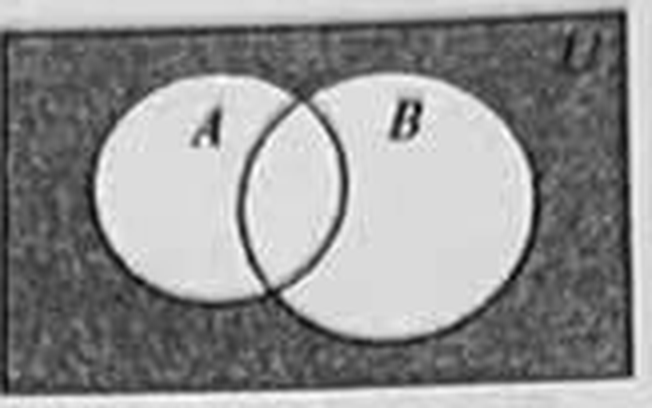
\includegraphics[width=0.30\textwidth]{figures/venn_AB_complement.png}
\end{center}

\ans{$\overline{A\cup B}$}

\ifanswer
\solbegin
\step{图中阴影部分在集合 $A$、$B$ 的外部，即在全集 $U$ 中但不属于 $A$、也不属于 $B$.}
\step{这正是 $A\cup B$ 在全集 $U$ 中的补集，故可表示为 $\overline{A\cup B}$（即 $\complement_U(A\cup B)$）.}
\solend

\fi

\item 设全集 $U=\R$，集合 $A=\{x\mid 2\leqslant x<5\}$，$B=\{x\mid 3<x<6\}$，则 $\overline{A}\cap B=$ \blankline[4.4em]（用区间表示）.

\ans{$[5,6)$}

\ifanswer
\solbegin
\step{在全集 $\R$ 中，$\overline{A}=(-\infty,2)\cup[5,+\infty)$.}
\step{又 $B=(3,6)$，取两集合的公共部分得 $\overline{A}\cap B=[5,6)$.}
\solend

\fi

\item 用反证法证明“$a,b\in\N$，$ab$ 可被 5 整除，那么 $a,b$ 中至少有一个能被 5 整除”时应假设 \blankline[4.4em].

\ans{$a,b$ 都不能被 5 整除}

\ifanswer
\solbegin
\step{反证法需假设结论的反面成立.}
\step{“$a,b$ 中至少有一个能被 5 整除”的反面是“$a,b$ 中没有一个能被 5 整除”，即 $a,b$ 都不能被 5 整除.}
\solend

\fi

\item 满足 $M\subseteq\{a_1,a_2,a_3,a_4,a_5\}$，且 $M\cap\{a_1,a_2,a_3\}=\{a_1,a_2\}$，则集合 $M$ 的个数是 \blankline[2.4em].

\ans{$4$}

\ifanswer
\solbegin
\step{由 $M\cap\{a_1,a_2,a_3\}=\{a_1,a_2\}$ 得 $a_1\in M$，$a_2\in M$，$a_3\notin M$.}
\step{又 $M\subseteq\{a_1,a_2,a_3,a_4,a_5\}$，所以 $a_4$、$a_5$ 可以属于 $M$，也可以不属于 $M$.}
\step{即 $M=\{a_1,a_2\}\cup S$，其中 $S\subseteq\{a_4,a_5\}$，共有 $2^2=4$ 个.}
\solend

\fi

\item 已知集合 $A=\{(x,y)\mid y=x^2\}$，$B=\left\{(x,y)\mid \dfrac{y-1}{x-1}=\dfrac{1}{2}\right\}$，则 $A\cap B=$ \blankline[5.2em].

\ans{$\left\{\left(-\dfrac{1}{2},\dfrac{1}{4}\right)\right\}$}

\ifanswer
\solbegin
\step{集合 $B$ 中的点满足 $y=\dfrac{1}{2}x+\dfrac{1}{2}$，且 $x\neq 1$.}
\step{代入 $y=x^2$ 得 $2x^2-x-1=0$，解得 $x=1$ 或 $x=-\dfrac{1}{2}$.}
\step{因为 $x\neq 1$，所以 $x=-\dfrac{1}{2}$，此时 $y=\dfrac{1}{4}$.}
\step{所以 $A\cap B=\left\{\left(-\dfrac{1}{2},\dfrac{1}{4}\right)\right\}$.}
\solend

\fi

\item 已知集合 $\{a,b,c\}=\{0,1,2\}$，且下列三个关系：①$a\neq 2$ ②$b=2$ ③$c\neq 0$ 有且只有一个正确，则 $100a+10b+c$ 等于 \blankline[2.4em].

\ans{$201$}

\ifanswer
\solbegin
\step{$a,b,c$ 是 $0,1,2$ 的一个排列，共 6 种情形，逐一检验三个关系的真假：}
\step{$(a,b,c)=(0,1,2)$：①真、②假、③真，两个正确，不合；$(0,2,1)$：三个都真，不合；}
\step{$(1,0,2)$：①真、②假、③真，两个正确，不合；$(1,2,0)$：①真、②真、③假，两个正确，不合；}
\step{$(2,0,1)$：①假、②假、③真，恰有一个正确，符合；$(2,1,0)$：三个都假，不合.}
\step{所以 $(a,b,c)=(2,0,1)$，$100a+10b+c=200+0+1=201$.}
\solend

\fi

\item “$x_1>3$ 且 $x_2>3$”是“$x_1+x_2>6$ 且 $x_1x_2>9$”的 \blankline[4.4em] 条件.（选填“充分非必要”，“必要非充分”，“充要”，“既非充分也非必要”）

\ans{充分非必要}

\ifanswer
\solbegin
\step{充分性：若 $x_1>3$ 且 $x_2>3$，则 $x_1+x_2>6$，且 $x_1x_2>9$，故充分性成立.}
\step{必要性：取 $x_1=2$、$x_2=5$，有 $x_1+x_2=7>6$、$x_1x_2=10>9$，但 $x_1>3$ 不成立，故必要性不成立.}
\step{所以应填“充分非必要”.}
\solend

\fi

% 注：第 11 题系 2010 年上海高考理科第 14 题的改写（原题要求选出 4 个子集，官方答案 36）。
%     原题官方解答明言「A、B 可以互换，即视为一种选法」，即**不计先后**计数；
%     按此口径本改写题的答案为 5。（原卷学生作答为 10，是把 A⊆B 与 B⊆A 重复计入。）
\item 在集合 $U=\{a,b,c,d\}$ 的子集中选出 2 个不同的子集，需同时满足以下两个条件：(1)$a,b$ 都要选出 (2)对选出的任意两个子集 $A$ 和 $B$，必有 $A\subseteq B$ 或 $B\subseteq A$，那么共有 \blankline[2.4em] 种不同的选法.

\ans{$5$}

\ifanswer
\solbegin
\step{由 (1) 知 $a,b$ 都要选出，即 $a,b$ 都属于所选的两个子集；由 (2) 知所选的两个子集必须可比.}
\step{含 $a,b$ 的子集只有 $\{a,b\}$、$\{a,b,c\}$、$\{a,b,d\}$、$\{a,b,c,d\}$ 共 4 个.}
\step{在这 4 个子集中取出两个不同的且可比的（一个包含另一个），只有下列 5 组：}
\step{$\{a,b\}\subset\{a,b,c\}$、$\{a,b\}\subset\{a,b,d\}$、$\{a,b\}\subset\{a,b,c,d\}$、$\{a,b,c\}\subset\{a,b,c,d\}$、$\{a,b,d\}\subset\{a,b,c,d\}$.}
\step{注意「选出 2 个子集」的选法\textbf{不计先后}：把这两个子集分别叫作 $A$、$B$ 只是给它们取个名字，$A\subseteq B$ 与 $B\subseteq A$ 说的是同一组子集，算同一种选法.}
\step{（本题由 2010 年上海高考理科第 14 题改写，原题要求选出 4 个子集，其官方答案 36 正是按「$A$、$B$ 可以互换，即视为一种选法」的不计先后口径计数.）}
\step{所以共有 5 种不同的选法.}
\solend

\fi

\end{enumerate}

\bigsec{二、选择题}

\begin{enumerate}
\setcounter{enumi}{11}

\item 已知 $M=(-\infty,\sqrt{3}]$，$a=\sqrt{3}$，则下列关系中正确的是（\quad）.

A. $a\subset M$\qquad B. $a\in M$\qquad C. $\{a\}\in M$\qquad D. $M\subset\{a\}$

\ans{B}

\ifanswer
\solbegin
\step{因为 $\sqrt{3}\leqslant\sqrt{3}$，所以 $a=\sqrt{3}\in M$，B 正确.}
\step{$a$ 是元素、$M$ 是集合，元素与集合之间用 $\in$ 表示，不能用 $\subset$，故 A、D 错误；}
\step{$\{a\}$ 是集合，集合与集合之间应是包含关系（且 $\{a\}\subseteq M$），不能用 $\in$，故 C 错误.}
\step{故选 B.}
\solend

\fi

% 注：原卷此处印作“已知集合{(x,y)|x^2+y^2≤3, x∈Z, y∈Z}”，集合未记作 A，
%     却设问“则 A 中的元素个数是”，显系漏排“A=”；本稿补上，其余照原卷。
\item 已知集合 $A=\{(x,y)\mid x^2+y^2\leqslant 3,\ x\in\Z,\ y\in\Z\}$，则 $A$ 中的元素个数是（\quad）.

A. $9$\qquad B. $8$\qquad C. $5$\qquad D. $4$

\ans{A}

\ifanswer
\solbegin
\step{逐一列举：$x=0$ 时 $y^2\leqslant 3$，$y=-1,0,1$，得 $(0,-1),(0,0),(0,1)$，共 3 个；}
\step{$x=\pm 1$ 时 $y^2\leqslant 2$，$y=-1,0,1$，各得 3 个，共 6 个（$x^2+y^2=2\leqslant 3$ 满足条件）；}
\step{$|x|\geqslant 2$ 时 $x^2\geqslant 4>3$，无解.}
\step{所以 $A$ 中元素个数为 $3+6=9$. 故选 A.}
\solend

\fi

\item 集合 $A=\{x\mid x=(2k-1)\pi,\ k\in\Z\}$ 与 $B=\{x\mid x=(4n\pm 1)\pi,\ n\in\Z\}$ 之间的关系是（\quad）.

A. $A\subset B$\qquad B. $B\subset A$\qquad C. $A=B$\qquad D. 不确定

\ans{C}

\ifanswer
\solbegin
\step{$A$ 由 $\pi$ 的一切奇数倍组成，即 $A=\{\cdots,-3\pi,-\pi,\pi,3\pi,\cdots\}$.}
\step{$B$ 中 $4n+1$ 与 $4n-1$ （$n\in\Z$）都是奇数，故 $B\subseteq A$；}
\step{反之，任一奇数除以 4 的余数只能是 1 或 3：形如 $4m+1$ 的奇数含于 $B$（取 $n=m$），形如 $4m+3=4(m+1)-1$ 的奇数也含于 $B$（取 $n=m+1$），所以 $A\subseteq B$.}
\step{于是 $A\subseteq B$ 且 $B\subseteq A$，即 $A=B$. 故选 C.}
\solend

\fi

\item 设 $T$ 是由正三角形 $P_1P_2P_3$ 边上及其内部的点构成的集合，点 $O$ 是 $\triangle P_1P_2P_3$ 的中心. 若集合 $S=\{P\mid P\in T,\ |PO|\leqslant|PO_i|,\ i=1,2,3\}$，（符号 $|AB|$ 表示平面上两点 $A,B$ 间的距离），则集合 $S$ 表示的平面区域是（\quad）.

A. 四边形区域；\qquad B. 三角形区域；\qquad C. 六边形区域；\qquad D. 五边形区域；

\ans{C}

\ifanswer
\solbegin
\step{$|PO|\leqslant|PO_i|$ 表示点 $P$ 到 $O$ 的距离不大于到顶点 $P_i$ 的距离，即 $P$ 落在线段 $OP_i$ 的垂直平分线靠 $O$ 的那一侧（含该线）.}
\step{对 $i=1,2,3$ 各有一条这样的直线，它们分别把三角形靠近 $P_1$、$P_2$、$P_3$ 的一个小角（三角形）截掉；}
\step{逐一直观验证可知这三条直线两两的交点都在三角形内部，三个角互不重叠，截去三个角后剩下的区域共有 6 条边.}
\step{所以集合 $S$ 表示的平面区域是六边形区域. 故选 C.}
\solend

\fi

\end{enumerate}

\bigsec{三、解答题}

\begin{enumerate}
\setcounter{enumi}{15}

\item（10 分，第 1 小问 5 分，第 2 小问 5 分）已知集合 $A=\{x\mid a\leqslant x\leqslant a+2\}$，集合 $B=\{x\mid x<-1\text{ 或 }x>5\}$，全集 $U=\R$.

\begin{enumerate}[label=(\arabic*)]
\item 若 $a=1$，求 $\overline{A}\cup B$；
\item 若 $A\subseteq B$，求实数 $a$ 的取值范围.
\end{enumerate}

\ans{（1）$(-\infty,1)\cup(3,+\infty)$；（2）$(-\infty,-3)\cup(5,+\infty)$}

\ifanswer
\solbegin
\stepm{(1)}{$a=1$ 时 $A=\{x\mid 1\leqslant x\leqslant 3\}=[1,3]$，则 $\overline{A}=(-\infty,1)\cup(3,+\infty)$.}
\step{又 $B=(-\infty,-1)\cup(5,+\infty)$，而 $B\subseteq\overline{A}$（因 $5>3$、$-1<1$），}
\step{所以 $\overline{A}\cup B=(-\infty,1)\cup(3,+\infty)$.}
\stepm{(2)}{因为 $a\leqslant a+2$，所以集合 $A=\{x\mid a\leqslant x\leqslant a+2\}$ 始终非空.}
\step{要使 $A\subseteq B$，只需 $A$ 与 $[-1,5]$ 没有公共点，即 $a+2<-1$ 或 $a>5$.}
\step{解得 $a<-3$ 或 $a>5$，所以实数 $a$ 的取值范围是 $(-\infty,-3)\cup(5,+\infty)$.}
\solend

\fi

\ansspace[10]

\item（10 分，第 1 小问 5 分，第 2 小问 5 分）已知 $A=\{x\mid x^2+x-2=0\}$，$B=\{x\mid x^2+ax+2a-4=0\}$.

\begin{enumerate}[label=(\arabic*)]
\item 若 $A=B$，求实数 $a$ 的值；
\item 若 $B\subseteq A$，求实数 $a$ 的值.
\end{enumerate}

\ans{（1）$a=1$；（2）$a=1$ 或 $a=4$}

\ifanswer
\solbegin
\stepm{(1)}{由 $x^2+x-2=0$ 解得 $x=1$ 或 $x=-2$，所以 $A=\{1,-2\}$.}
\step{由 $A=B$ 知 $1$、$-2$ 是方程 $x^2+ax+2a-4=0$ 的两根，由根与系数的关系得 $1+(-2)=-a$，所以 $a=1$；}
\step{此时 $2a-4=-2=1\times(-2)$，与两根之积相符，故 $a=1$.}
\stepm{(2)}{方程 $x^2+ax+2a-4=0$ 的判别式 $\Delta=a^2-4(2a-4)=(a-4)^2\geqslant 0$ 恒成立，所以集合 $B$ 不可能是空集.}
\step{由 $B\subseteq A$ 知 $B=\{1\}$ 或 $B=\{-2\}$ 或 $B=\{1,-2\}$.}
\step{若 $B=\{1\}$，则 $1$ 是二重根，$1+1=-a$ 且 $1\times 1=2a-4$，即 $a=-2$ 且 $a=\dfrac{5}{2}$，无解；}
\step{若 $B=\{-2\}$，则 $-2$ 是二重根，$(-2)+(-2)=-a$ 且 $(-2)\times(-2)=2a-4$，两式都给出 $a=4$，符合；}
\step{若 $B=\{1,-2\}$，则 $1+(-2)=-a$，得 $a=1$，此时 $2a-4=-2=1\times(-2)$，符合.}
\step{综上，$a=1$ 或 $a=4$.}
\solend

\fi

\ansspace[12]

\item（11 分，第 1 小问 3 分，第 2 小问 3 分，第 3 小问 5 分）已知非空数集 $S$ 满足：对任意给定的 $x,y\in S$（$x,y$ 可以相同），有 $x+y\in S$ 且 $x-y\in S$.

\begin{enumerate}[label=(\arabic*)]
\item 哪个数一定是 $S$ 中的元素?说明理由；
\item 若 $S$ 是有限集，求 $S$；
\item 若 $S$ 中最小的正数为 5，求 $S$.
\end{enumerate}

\ans{（1）$0$；（2）$S=\{0\}$；（3）$S=\{x\mid x=5a,\ a\in\Z\}$}

\ifanswer
\solbegin
\stepm{(1)}{$0$ 一定是 $S$ 中的元素. 理由：$S$ 非空，取 $x\in S$，在 $x-y\in S$ 中令 $y=x$（$x,y$ 可以相同），得 $x-x=0\in S$.}
\stepm{(2)}{若 $S$ 是有限集，则 $S=\{0\}$. 理由：取 $x\in S$ 且 $x\neq 0$，由 $x+y\in S$ 依次得 $2x=x+x\in S$，$3x=2x+x\in S$，$\cdots$，即 $kx\in S$（$k=1,2,3,\cdots$）；}
\step{这些数互不相同，与 $S$ 是有限集矛盾，所以 $S$ 中除 $0$ 外没有别的元素，即 $S=\{0\}$（此时 $0+0=0\in S$，$0-0=0\in S$，符合条件）.}
\stepm{(3)}{因为 $5\in S$，由 $x+y\in S$ 得 $5+5=10\in S$，$10+5=15\in S$，$\cdots$，故一切正整数倍的 $5$ 都在 $S$ 中；}
\step{又由 $x-y\in S$ 得 $5-5=0\in S$，$0-5=-5\in S$，$-5-5=-10\in S$，$\cdots$，故一切负整数倍的 $5$ 也都在 $S$ 中，即 $\{5a\mid a\in\Z\}\subseteq S$.}
\step{反之，任取 $s\in S$，由 $5\in S$ 及封闭性知 $s-5k\in S$（$k\in\Z$）；把 $s$ 写成 $s=5q+r$（$q\in\Z$，$0\leqslant r<5$），取 $k=q$ 得 $r=s-5q\in S$.}
\step{若 $r>0$，则 $S$ 中有比 $5$ 更小的正数 $r$，与“$S$ 中最小的正数为 5”矛盾，故只能 $r=0$，即 $s=5q$.}
\step{所以 $S=\{x\mid x=5a,\ a\in\Z\}$.}
\solend

\fi

\ansspace[12]

\end{enumerate}

\bigsec{附加题}

\begin{enumerate}
\setcounter{enumi}{18}

\item 已知集合 $A,B,C\subseteq\{1,2,3,\cdots,2024\}$，且 $A\subseteq B\subseteq C$，则有序集合组 $(A,B,C)$ 的个数是 \blankline[3.2em].

\ans{$4^{2024}$}

\ifanswer
\solbegin
\step{对 $U=\{1,2,\cdots,2024\}$ 中的每个元素，它与 $A,B,C$ 的关系只有四种可能：}
\step{在 $A,B,C$ 中都出现；不在 $A$ 中而在 $B,C$ 中出现；只在 $C$ 中出现；在三个集合中都不出现.}
\step{反过来，任取每个元素的一种归属方式，都恰好得到一个满足 $A\subseteq B\subseteq C$ 的有序集合组，故不同的组与不同的归属方式一一对应.}
\step{所以共有 $4\times 4\times\cdots\times 4=4^{2024}$ 个有序集合组.}
\solend

\fi

\item 已知集合 $M=\{1,2,\cdots,10\}$，对它的非空子集 $A$，将 $A$ 中的每个元素 $k$ 都乘以 $(-1)^k$ 再求和，如 $A=\{2,3,6\}$，可求得和为 $(-1)^2\times 2+(-1)^3\times 3+(-1)^6\times 6=5$. 试对 $M$ 的所有非空子集，求这些和的总和 \blankline[3.2em].

\ans{$2560$}

\ifanswer
\solbegin
\step{元素 $k$（$k=1,2,\cdots,10$）出现在 $M$ 的 $2^{9}$ 个非空子集中（其余 9 个元素任取）.}
\step{所以在所有非空子集的和中，$k$ 贡献的总量为 $2^{9}\times(-1)^k\cdot k=512\times(-1)^kk$.}
\step{于是这些和的总和为 $512\displaystyle\sum_{k=1}^{10}(-1)^kk=512\times(-1+2-3+4-5+6-7+8-9+10)=512\times 5=2560$.}
\solend

\fi

\item 设 $a_1,a_2,a_3,a_4$ 是 4 个有理数，使得 $\{a_ia_j\mid 1\leqslant i<j\leqslant 4\}=\left\{-24,-2,-\dfrac{3}{2},-\dfrac{1}{8},1,3\right\}$. 求 $a_1+a_2+a_3+a_4=$ \blankline[3.2em].

\ans{$\pm\dfrac{9}{4}$（两组解，和分别为 $-\dfrac{9}{4}$ 与 $\dfrac{9}{4}$）}

\ifanswer
\solbegin
\step{六个乘积中有 4 个负数、2 个正数. 设 4 个数中正数有 $p$ 个、负数有 $q$ 个（$p+q=4$），则异号的两数相乘得负数，其个数为 $pq$；由 $pq=4$ 得 $p=q=2$，即恰有 2 个正数、2 个负数.}
\step{把 4 个数的绝对值记作 $w,x,y,z>0$，则六个两两乘积的绝对值为 $24,2,\dfrac{3}{2},\dfrac{1}{8},1,3$；其中 $1$ 与 $3$ 来自两对同号的数，$24,2,\dfrac{3}{2},\dfrac{1}{8}$ 来自四对异号的数.}
\step{由 $(a_1a_2a_3a_4)^3=(-24)\times(-2)\times\left(-\dfrac{3}{2}\right)\times\left(-\dfrac{1}{8}\right)\times 1\times 3=27$ 得 $a_1a_2a_3a_4=3$，即去符号后 $wxyz=3$.}
\step{逐一检验可知 $w,x,y,z$ 只能是 $\left\{4,\dfrac{1}{4},6,\dfrac{1}{2}\right\}$：其中 $4\times\dfrac{1}{4}=1$、$6\times\dfrac{1}{2}=3$ 为同号两对的乘积，$4\times 6=24$、$4\times\dfrac{1}{2}=2$、$\dfrac{1}{4}\times 6=\dfrac{3}{2}$、$\dfrac{1}{4}\times\dfrac{1}{2}=\dfrac{1}{8}$ 为异号四对的乘积.}
\step{于是 $\left\{4,\dfrac{1}{4}\right\}$ 中的两个数同号、$\left\{6,\dfrac{1}{2}\right\}$ 中的两个数同号，且这两组异号，得两组解：}
\step{$4,\ \dfrac{1}{4},\ -6,\ -\dfrac{1}{2}$，和为 $-\dfrac{9}{4}$；\quad 或 \quad $6,\ \dfrac{1}{2},\ -4,\ -\dfrac{1}{4}$，和为 $\dfrac{9}{4}$.}
\step{两组解的六个乘积都恰为 $-24,-2,-\dfrac{3}{2},-\dfrac{1}{8},1,3$，与原卷所给集合相同.}
\step{所以 $a_1+a_2+a_3+a_4=\pm\dfrac{9}{4}$.}
\solend

\fi

\end{enumerate}

\end{document}
"
%
% 原始材料为学生作业的手机翻拍照片（卷面为学生本人的**手写作答**，未见教师批改痕迹）。
% 试题文字照原卷录入；答案版给出的是**经核验的正确解答与解析**，与原卷手写答案的差异见 README。
%
% 与原卷的两处排版差异（均已在 README「说明」中交代）：
%   ① 原卷未印分节标题与分值，本稿按题型补「一、填空题 / 二、选择题 / 三、解答题」三节
%      （「附加题」原卷有印）；
%   ② 第 13 题原卷印作「已知集合{(x,y)|…}」，集合未记作 A 却被设问为「A 中的元素个数」，
%      显系漏排「A=」，本稿补上。

% 本篇的正文与家长拍照卷 `高一b_大同中学_第二周周末练习1（补）` **完全相同**——同一份作业，
% 试卷版/答案版也都是同一份源码编译而来；`高一b` 的 4 张原图另存于
% `原图/高一b_大同中学_第二周周末练习1（补）/`，本卷 `原图/` 下是同一组照片的副本。
% 经核对，这份作业就是公众号「魔都数学加油站」连载「27学年高一16——2026-2027年上海市大同中学
% 高一上周末作业2.1」的那一份：**题号与题干逐题一致**，只是公众号版略去了填空第 1、2 题，
% 故拍照卷反而是更完整的版本（对照关系见 README「与公众号连载号的对照表」）。
%
% 本卷的编号与连载号对齐（高一16），卷面标题因此**不带**「（补）」；标题里的「大同中学」为**本稿所加**
% （原卷标题只有作业名，校名只印在页眉「上海市大同…」）。带「（补）」的 `高一b` 保留为
% 拍照原件的转录本，两者内容一字不差。
%
% 一处与公众号讲评版的差异需留意：本卷第 11 题的答案按 2010 年上海高考理科第 14 题官方解答
% 「A、B 可以互换，即视为一种选法」的不计先后口径取 5，而公众号讲评版把它按有先后的 32 计数
% （该题学生原作答为 10）。取舍理由见该题下的 `%` 注。
\documentclass[a4paper,11pt]{article}
\usepackage{common}

\begin{document}

\examtitlest[3]{2026--2027 学年度大同中学高一上数学第二周周末练习1}{集合与常用逻辑用语}

\bigsec{一、填空题}

\begin{enumerate}

\item 用列举法表示集合 $\{x\mid -2<x\leqslant 2,\ x\in\Z\}=$ \blankline[2.4em].

\ans{$\{-1,0,1,2\}$}

\ifanswer
\solbegin
\step{集合中的元素是满足 $-2<x\leqslant 2$ 的整数，即 $-1$、$0$、$1$、$2$.}
\step{所以用列举法表示为 $\{-1,0,1,2\}$.}
\solend

\fi

\item 设集合 $A=\{1,a\}$，$B=\{1,a^2\}$，若 $A=B$，则实数 $a$ 的值为 \blankline[2.4em].

\ans{$a=0$}

\ifanswer
\solbegin
\step{由 $A=B$ 得 $a^2=a$，解得 $a=0$ 或 $a=1$.}
\step{当 $a=1$ 时，$A=\{1,1\}$，不符合集合元素的互异性，舍去；}
\step{当 $a=0$ 时，$A=\{1,0\}$，$B=\{1,0\}$，两集合相等，符合条件.}
\step{所以 $a=0$.}
\solend

\fi

\item 已知集合 $A=\{0,2,3,4,5\}$，$B=\{2,3,5,7\}$，$C=\{2,3,6\}$，则 $(A\cap B)\cup C=$ \blankline[4.4em].

\ans{$\{2,3,5,6\}$}

\ifanswer
\solbegin
\step{$A\cap B=\{0,2,3,4,5\}\cap\{2,3,5,7\}=\{2,3,5\}$.}
\step{所以 $(A\cap B)\cup C=\{2,3,5\}\cup\{2,3,6\}=\{2,3,5,6\}$.}
\solend

\fi

\item 设全集为 $U$，用集合 $A,B$ 的交、并或补集符号表示图中的阴影部分是 \blankline[4.4em].

\begin{center}
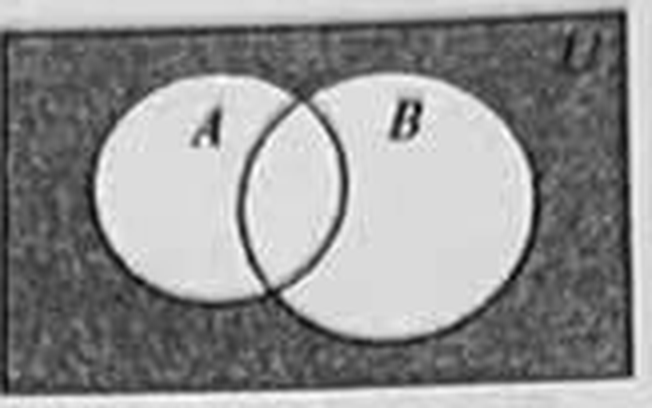
\includegraphics[width=0.30\textwidth]{figures/venn_AB_complement.png}
\end{center}

\ans{$\overline{A\cup B}$}

\ifanswer
\solbegin
\step{图中阴影部分在集合 $A$、$B$ 的外部，即在全集 $U$ 中但不属于 $A$、也不属于 $B$.}
\step{这正是 $A\cup B$ 在全集 $U$ 中的补集，故可表示为 $\overline{A\cup B}$（即 $\complement_U(A\cup B)$）.}
\solend

\fi

\item 设全集 $U=\R$，集合 $A=\{x\mid 2\leqslant x<5\}$，$B=\{x\mid 3<x<6\}$，则 $\overline{A}\cap B=$ \blankline[4.4em]（用区间表示）.

\ans{$[5,6)$}

\ifanswer
\solbegin
\step{在全集 $\R$ 中，$\overline{A}=(-\infty,2)\cup[5,+\infty)$.}
\step{又 $B=(3,6)$，取两集合的公共部分得 $\overline{A}\cap B=[5,6)$.}
\solend

\fi

\item 用反证法证明“$a,b\in\N$，$ab$ 可被 5 整除，那么 $a,b$ 中至少有一个能被 5 整除”时应假设 \blankline[4.4em].

\ans{$a,b$ 都不能被 5 整除}

\ifanswer
\solbegin
\step{反证法需假设结论的反面成立.}
\step{“$a,b$ 中至少有一个能被 5 整除”的反面是“$a,b$ 中没有一个能被 5 整除”，即 $a,b$ 都不能被 5 整除.}
\solend

\fi

\item 满足 $M\subseteq\{a_1,a_2,a_3,a_4,a_5\}$，且 $M\cap\{a_1,a_2,a_3\}=\{a_1,a_2\}$，则集合 $M$ 的个数是 \blankline[2.4em].

\ans{$4$}

\ifanswer
\solbegin
\step{由 $M\cap\{a_1,a_2,a_3\}=\{a_1,a_2\}$ 得 $a_1\in M$，$a_2\in M$，$a_3\notin M$.}
\step{又 $M\subseteq\{a_1,a_2,a_3,a_4,a_5\}$，所以 $a_4$、$a_5$ 可以属于 $M$，也可以不属于 $M$.}
\step{即 $M=\{a_1,a_2\}\cup S$，其中 $S\subseteq\{a_4,a_5\}$，共有 $2^2=4$ 个.}
\solend

\fi

\item 已知集合 $A=\{(x,y)\mid y=x^2\}$，$B=\left\{(x,y)\mid \dfrac{y-1}{x-1}=\dfrac{1}{2}\right\}$，则 $A\cap B=$ \blankline[5.2em].

\ans{$\left\{\left(-\dfrac{1}{2},\dfrac{1}{4}\right)\right\}$}

\ifanswer
\solbegin
\step{集合 $B$ 中的点满足 $y=\dfrac{1}{2}x+\dfrac{1}{2}$，且 $x\neq 1$.}
\step{代入 $y=x^2$ 得 $2x^2-x-1=0$，解得 $x=1$ 或 $x=-\dfrac{1}{2}$.}
\step{因为 $x\neq 1$，所以 $x=-\dfrac{1}{2}$，此时 $y=\dfrac{1}{4}$.}
\step{所以 $A\cap B=\left\{\left(-\dfrac{1}{2},\dfrac{1}{4}\right)\right\}$.}
\solend

\fi

\item 已知集合 $\{a,b,c\}=\{0,1,2\}$，且下列三个关系：①$a\neq 2$ ②$b=2$ ③$c\neq 0$ 有且只有一个正确，则 $100a+10b+c$ 等于 \blankline[2.4em].

\ans{$201$}

\ifanswer
\solbegin
\step{$a,b,c$ 是 $0,1,2$ 的一个排列，共 6 种情形，逐一检验三个关系的真假：}
\step{$(a,b,c)=(0,1,2)$：①真、②假、③真，两个正确，不合；$(0,2,1)$：三个都真，不合；}
\step{$(1,0,2)$：①真、②假、③真，两个正确，不合；$(1,2,0)$：①真、②真、③假，两个正确，不合；}
\step{$(2,0,1)$：①假、②假、③真，恰有一个正确，符合；$(2,1,0)$：三个都假，不合.}
\step{所以 $(a,b,c)=(2,0,1)$，$100a+10b+c=200+0+1=201$.}
\solend

\fi

\item “$x_1>3$ 且 $x_2>3$”是“$x_1+x_2>6$ 且 $x_1x_2>9$”的 \blankline[4.4em] 条件.（选填“充分非必要”，“必要非充分”，“充要”，“既非充分也非必要”）

\ans{充分非必要}

\ifanswer
\solbegin
\step{充分性：若 $x_1>3$ 且 $x_2>3$，则 $x_1+x_2>6$，且 $x_1x_2>9$，故充分性成立.}
\step{必要性：取 $x_1=2$、$x_2=5$，有 $x_1+x_2=7>6$、$x_1x_2=10>9$，但 $x_1>3$ 不成立，故必要性不成立.}
\step{所以应填“充分非必要”.}
\solend

\fi

% 注：第 11 题系 2010 年上海高考理科第 14 题的改写（原题要求选出 4 个子集，官方答案 36）。
%     原题官方解答明言「A、B 可以互换，即视为一种选法」，即**不计先后**计数；
%     按此口径本改写题的答案为 5。（原卷学生作答为 10，是把 A⊆B 与 B⊆A 重复计入。）
\item 在集合 $U=\{a,b,c,d\}$ 的子集中选出 2 个不同的子集，需同时满足以下两个条件：(1)$a,b$ 都要选出 (2)对选出的任意两个子集 $A$ 和 $B$，必有 $A\subseteq B$ 或 $B\subseteq A$，那么共有 \blankline[2.4em] 种不同的选法.

\ans{$5$}

\ifanswer
\solbegin
\step{由 (1) 知 $a,b$ 都要选出，即 $a,b$ 都属于所选的两个子集；由 (2) 知所选的两个子集必须可比.}
\step{含 $a,b$ 的子集只有 $\{a,b\}$、$\{a,b,c\}$、$\{a,b,d\}$、$\{a,b,c,d\}$ 共 4 个.}
\step{在这 4 个子集中取出两个不同的且可比的（一个包含另一个），只有下列 5 组：}
\step{$\{a,b\}\subset\{a,b,c\}$、$\{a,b\}\subset\{a,b,d\}$、$\{a,b\}\subset\{a,b,c,d\}$、$\{a,b,c\}\subset\{a,b,c,d\}$、$\{a,b,d\}\subset\{a,b,c,d\}$.}
\step{注意「选出 2 个子集」的选法\textbf{不计先后}：把这两个子集分别叫作 $A$、$B$ 只是给它们取个名字，$A\subseteq B$ 与 $B\subseteq A$ 说的是同一组子集，算同一种选法.}
\step{（本题由 2010 年上海高考理科第 14 题改写，原题要求选出 4 个子集，其官方答案 36 正是按「$A$、$B$ 可以互换，即视为一种选法」的不计先后口径计数.）}
\step{所以共有 5 种不同的选法.}
\solend

\fi

\end{enumerate}

\bigsec{二、选择题}

\begin{enumerate}
\setcounter{enumi}{11}

\item 已知 $M=(-\infty,\sqrt{3}]$，$a=\sqrt{3}$，则下列关系中正确的是（\quad）.

A. $a\subset M$\qquad B. $a\in M$\qquad C. $\{a\}\in M$\qquad D. $M\subset\{a\}$

\ans{B}

\ifanswer
\solbegin
\step{因为 $\sqrt{3}\leqslant\sqrt{3}$，所以 $a=\sqrt{3}\in M$，B 正确.}
\step{$a$ 是元素、$M$ 是集合，元素与集合之间用 $\in$ 表示，不能用 $\subset$，故 A、D 错误；}
\step{$\{a\}$ 是集合，集合与集合之间应是包含关系（且 $\{a\}\subseteq M$），不能用 $\in$，故 C 错误.}
\step{故选 B.}
\solend

\fi

% 注：原卷此处印作“已知集合{(x,y)|x^2+y^2≤3, x∈Z, y∈Z}”，集合未记作 A，
%     却设问“则 A 中的元素个数是”，显系漏排“A=”；本稿补上，其余照原卷。
\item 已知集合 $A=\{(x,y)\mid x^2+y^2\leqslant 3,\ x\in\Z,\ y\in\Z\}$，则 $A$ 中的元素个数是（\quad）.

A. $9$\qquad B. $8$\qquad C. $5$\qquad D. $4$

\ans{A}

\ifanswer
\solbegin
\step{逐一列举：$x=0$ 时 $y^2\leqslant 3$，$y=-1,0,1$，得 $(0,-1),(0,0),(0,1)$，共 3 个；}
\step{$x=\pm 1$ 时 $y^2\leqslant 2$，$y=-1,0,1$，各得 3 个，共 6 个（$x^2+y^2=2\leqslant 3$ 满足条件）；}
\step{$|x|\geqslant 2$ 时 $x^2\geqslant 4>3$，无解.}
\step{所以 $A$ 中元素个数为 $3+6=9$. 故选 A.}
\solend

\fi

\item 集合 $A=\{x\mid x=(2k-1)\pi,\ k\in\Z\}$ 与 $B=\{x\mid x=(4n\pm 1)\pi,\ n\in\Z\}$ 之间的关系是（\quad）.

A. $A\subset B$\qquad B. $B\subset A$\qquad C. $A=B$\qquad D. 不确定

\ans{C}

\ifanswer
\solbegin
\step{$A$ 由 $\pi$ 的一切奇数倍组成，即 $A=\{\cdots,-3\pi,-\pi,\pi,3\pi,\cdots\}$.}
\step{$B$ 中 $4n+1$ 与 $4n-1$ （$n\in\Z$）都是奇数，故 $B\subseteq A$；}
\step{反之，任一奇数除以 4 的余数只能是 1 或 3：形如 $4m+1$ 的奇数含于 $B$（取 $n=m$），形如 $4m+3=4(m+1)-1$ 的奇数也含于 $B$（取 $n=m+1$），所以 $A\subseteq B$.}
\step{于是 $A\subseteq B$ 且 $B\subseteq A$，即 $A=B$. 故选 C.}
\solend

\fi

\item 设 $T$ 是由正三角形 $P_1P_2P_3$ 边上及其内部的点构成的集合，点 $O$ 是 $\triangle P_1P_2P_3$ 的中心. 若集合 $S=\{P\mid P\in T,\ |PO|\leqslant|PO_i|,\ i=1,2,3\}$，（符号 $|AB|$ 表示平面上两点 $A,B$ 间的距离），则集合 $S$ 表示的平面区域是（\quad）.

A. 四边形区域；\qquad B. 三角形区域；\qquad C. 六边形区域；\qquad D. 五边形区域；

\ans{C}

\ifanswer
\solbegin
\step{$|PO|\leqslant|PO_i|$ 表示点 $P$ 到 $O$ 的距离不大于到顶点 $P_i$ 的距离，即 $P$ 落在线段 $OP_i$ 的垂直平分线靠 $O$ 的那一侧（含该线）.}
\step{对 $i=1,2,3$ 各有一条这样的直线，它们分别把三角形靠近 $P_1$、$P_2$、$P_3$ 的一个小角（三角形）截掉；}
\step{逐一直观验证可知这三条直线两两的交点都在三角形内部，三个角互不重叠，截去三个角后剩下的区域共有 6 条边.}
\step{所以集合 $S$ 表示的平面区域是六边形区域. 故选 C.}
\solend

\fi

\end{enumerate}

\bigsec{三、解答题}

\begin{enumerate}
\setcounter{enumi}{15}

\item（10 分，第 1 小问 5 分，第 2 小问 5 分）已知集合 $A=\{x\mid a\leqslant x\leqslant a+2\}$，集合 $B=\{x\mid x<-1\text{ 或 }x>5\}$，全集 $U=\R$.

\begin{enumerate}[label=(\arabic*)]
\item 若 $a=1$，求 $\overline{A}\cup B$；
\item 若 $A\subseteq B$，求实数 $a$ 的取值范围.
\end{enumerate}

\ans{（1）$(-\infty,1)\cup(3,+\infty)$；（2）$(-\infty,-3)\cup(5,+\infty)$}

\ifanswer
\solbegin
\stepm{(1)}{$a=1$ 时 $A=\{x\mid 1\leqslant x\leqslant 3\}=[1,3]$，则 $\overline{A}=(-\infty,1)\cup(3,+\infty)$.}
\step{又 $B=(-\infty,-1)\cup(5,+\infty)$，而 $B\subseteq\overline{A}$（因 $5>3$、$-1<1$），}
\step{所以 $\overline{A}\cup B=(-\infty,1)\cup(3,+\infty)$.}
\stepm{(2)}{因为 $a\leqslant a+2$，所以集合 $A=\{x\mid a\leqslant x\leqslant a+2\}$ 始终非空.}
\step{要使 $A\subseteq B$，只需 $A$ 与 $[-1,5]$ 没有公共点，即 $a+2<-1$ 或 $a>5$.}
\step{解得 $a<-3$ 或 $a>5$，所以实数 $a$ 的取值范围是 $(-\infty,-3)\cup(5,+\infty)$.}
\solend

\fi

\ansspace[10]

\item（10 分，第 1 小问 5 分，第 2 小问 5 分）已知 $A=\{x\mid x^2+x-2=0\}$，$B=\{x\mid x^2+ax+2a-4=0\}$.

\begin{enumerate}[label=(\arabic*)]
\item 若 $A=B$，求实数 $a$ 的值；
\item 若 $B\subseteq A$，求实数 $a$ 的值.
\end{enumerate}

\ans{（1）$a=1$；（2）$a=1$ 或 $a=4$}

\ifanswer
\solbegin
\stepm{(1)}{由 $x^2+x-2=0$ 解得 $x=1$ 或 $x=-2$，所以 $A=\{1,-2\}$.}
\step{由 $A=B$ 知 $1$、$-2$ 是方程 $x^2+ax+2a-4=0$ 的两根，由根与系数的关系得 $1+(-2)=-a$，所以 $a=1$；}
\step{此时 $2a-4=-2=1\times(-2)$，与两根之积相符，故 $a=1$.}
\stepm{(2)}{方程 $x^2+ax+2a-4=0$ 的判别式 $\Delta=a^2-4(2a-4)=(a-4)^2\geqslant 0$ 恒成立，所以集合 $B$ 不可能是空集.}
\step{由 $B\subseteq A$ 知 $B=\{1\}$ 或 $B=\{-2\}$ 或 $B=\{1,-2\}$.}
\step{若 $B=\{1\}$，则 $1$ 是二重根，$1+1=-a$ 且 $1\times 1=2a-4$，即 $a=-2$ 且 $a=\dfrac{5}{2}$，无解；}
\step{若 $B=\{-2\}$，则 $-2$ 是二重根，$(-2)+(-2)=-a$ 且 $(-2)\times(-2)=2a-4$，两式都给出 $a=4$，符合；}
\step{若 $B=\{1,-2\}$，则 $1+(-2)=-a$，得 $a=1$，此时 $2a-4=-2=1\times(-2)$，符合.}
\step{综上，$a=1$ 或 $a=4$.}
\solend

\fi

\ansspace[12]

\item（11 分，第 1 小问 3 分，第 2 小问 3 分，第 3 小问 5 分）已知非空数集 $S$ 满足：对任意给定的 $x,y\in S$（$x,y$ 可以相同），有 $x+y\in S$ 且 $x-y\in S$.

\begin{enumerate}[label=(\arabic*)]
\item 哪个数一定是 $S$ 中的元素?说明理由；
\item 若 $S$ 是有限集，求 $S$；
\item 若 $S$ 中最小的正数为 5，求 $S$.
\end{enumerate}

\ans{（1）$0$；（2）$S=\{0\}$；（3）$S=\{x\mid x=5a,\ a\in\Z\}$}

\ifanswer
\solbegin
\stepm{(1)}{$0$ 一定是 $S$ 中的元素. 理由：$S$ 非空，取 $x\in S$，在 $x-y\in S$ 中令 $y=x$（$x,y$ 可以相同），得 $x-x=0\in S$.}
\stepm{(2)}{若 $S$ 是有限集，则 $S=\{0\}$. 理由：取 $x\in S$ 且 $x\neq 0$，由 $x+y\in S$ 依次得 $2x=x+x\in S$，$3x=2x+x\in S$，$\cdots$，即 $kx\in S$（$k=1,2,3,\cdots$）；}
\step{这些数互不相同，与 $S$ 是有限集矛盾，所以 $S$ 中除 $0$ 外没有别的元素，即 $S=\{0\}$（此时 $0+0=0\in S$，$0-0=0\in S$，符合条件）.}
\stepm{(3)}{因为 $5\in S$，由 $x+y\in S$ 得 $5+5=10\in S$，$10+5=15\in S$，$\cdots$，故一切正整数倍的 $5$ 都在 $S$ 中；}
\step{又由 $x-y\in S$ 得 $5-5=0\in S$，$0-5=-5\in S$，$-5-5=-10\in S$，$\cdots$，故一切负整数倍的 $5$ 也都在 $S$ 中，即 $\{5a\mid a\in\Z\}\subseteq S$.}
\step{反之，任取 $s\in S$，由 $5\in S$ 及封闭性知 $s-5k\in S$（$k\in\Z$）；把 $s$ 写成 $s=5q+r$（$q\in\Z$，$0\leqslant r<5$），取 $k=q$ 得 $r=s-5q\in S$.}
\step{若 $r>0$，则 $S$ 中有比 $5$ 更小的正数 $r$，与“$S$ 中最小的正数为 5”矛盾，故只能 $r=0$，即 $s=5q$.}
\step{所以 $S=\{x\mid x=5a,\ a\in\Z\}$.}
\solend

\fi

\ansspace[12]

\end{enumerate}

\bigsec{附加题}

\begin{enumerate}
\setcounter{enumi}{18}

\item 已知集合 $A,B,C\subseteq\{1,2,3,\cdots,2024\}$，且 $A\subseteq B\subseteq C$，则有序集合组 $(A,B,C)$ 的个数是 \blankline[3.2em].

\ans{$4^{2024}$}

\ifanswer
\solbegin
\step{对 $U=\{1,2,\cdots,2024\}$ 中的每个元素，它与 $A,B,C$ 的关系只有四种可能：}
\step{在 $A,B,C$ 中都出现；不在 $A$ 中而在 $B,C$ 中出现；只在 $C$ 中出现；在三个集合中都不出现.}
\step{反过来，任取每个元素的一种归属方式，都恰好得到一个满足 $A\subseteq B\subseteq C$ 的有序集合组，故不同的组与不同的归属方式一一对应.}
\step{所以共有 $4\times 4\times\cdots\times 4=4^{2024}$ 个有序集合组.}
\solend

\fi

\item 已知集合 $M=\{1,2,\cdots,10\}$，对它的非空子集 $A$，将 $A$ 中的每个元素 $k$ 都乘以 $(-1)^k$ 再求和，如 $A=\{2,3,6\}$，可求得和为 $(-1)^2\times 2+(-1)^3\times 3+(-1)^6\times 6=5$. 试对 $M$ 的所有非空子集，求这些和的总和 \blankline[3.2em].

\ans{$2560$}

\ifanswer
\solbegin
\step{元素 $k$（$k=1,2,\cdots,10$）出现在 $M$ 的 $2^{9}$ 个非空子集中（其余 9 个元素任取）.}
\step{所以在所有非空子集的和中，$k$ 贡献的总量为 $2^{9}\times(-1)^k\cdot k=512\times(-1)^kk$.}
\step{于是这些和的总和为 $512\displaystyle\sum_{k=1}^{10}(-1)^kk=512\times(-1+2-3+4-5+6-7+8-9+10)=512\times 5=2560$.}
\solend

\fi

\item 设 $a_1,a_2,a_3,a_4$ 是 4 个有理数，使得 $\{a_ia_j\mid 1\leqslant i<j\leqslant 4\}=\left\{-24,-2,-\dfrac{3}{2},-\dfrac{1}{8},1,3\right\}$. 求 $a_1+a_2+a_3+a_4=$ \blankline[3.2em].

\ans{$\pm\dfrac{9}{4}$（两组解，和分别为 $-\dfrac{9}{4}$ 与 $\dfrac{9}{4}$）}

\ifanswer
\solbegin
\step{六个乘积中有 4 个负数、2 个正数. 设 4 个数中正数有 $p$ 个、负数有 $q$ 个（$p+q=4$），则异号的两数相乘得负数，其个数为 $pq$；由 $pq=4$ 得 $p=q=2$，即恰有 2 个正数、2 个负数.}
\step{把 4 个数的绝对值记作 $w,x,y,z>0$，则六个两两乘积的绝对值为 $24,2,\dfrac{3}{2},\dfrac{1}{8},1,3$；其中 $1$ 与 $3$ 来自两对同号的数，$24,2,\dfrac{3}{2},\dfrac{1}{8}$ 来自四对异号的数.}
\step{由 $(a_1a_2a_3a_4)^3=(-24)\times(-2)\times\left(-\dfrac{3}{2}\right)\times\left(-\dfrac{1}{8}\right)\times 1\times 3=27$ 得 $a_1a_2a_3a_4=3$，即去符号后 $wxyz=3$.}
\step{逐一检验可知 $w,x,y,z$ 只能是 $\left\{4,\dfrac{1}{4},6,\dfrac{1}{2}\right\}$：其中 $4\times\dfrac{1}{4}=1$、$6\times\dfrac{1}{2}=3$ 为同号两对的乘积，$4\times 6=24$、$4\times\dfrac{1}{2}=2$、$\dfrac{1}{4}\times 6=\dfrac{3}{2}$、$\dfrac{1}{4}\times\dfrac{1}{2}=\dfrac{1}{8}$ 为异号四对的乘积.}
\step{于是 $\left\{4,\dfrac{1}{4}\right\}$ 中的两个数同号、$\left\{6,\dfrac{1}{2}\right\}$ 中的两个数同号，且这两组异号，得两组解：}
\step{$4,\ \dfrac{1}{4},\ -6,\ -\dfrac{1}{2}$，和为 $-\dfrac{9}{4}$；\quad 或 \quad $6,\ \dfrac{1}{2},\ -4,\ -\dfrac{1}{4}$，和为 $\dfrac{9}{4}$.}
\step{两组解的六个乘积都恰为 $-24,-2,-\dfrac{3}{2},-\dfrac{1}{8},1,3$，与原卷所给集合相同.}
\step{所以 $a_1+a_2+a_3+a_4=\pm\dfrac{9}{4}$.}
\solend

\fi

\end{enumerate}

\end{document}
"
%
% 原始材料为学生作业的手机翻拍照片（卷面为学生本人的**手写作答**，未见教师批改痕迹）。
% 试题文字照原卷录入；答案版给出的是**经核验的正确解答与解析**，与原卷手写答案的差异见 README。
%
% 与原卷的两处排版差异（均已在 README「说明」中交代）：
%   ① 原卷未印分节标题与分值，本稿按题型补「一、填空题 / 二、选择题 / 三、解答题」三节
%      （「附加题」原卷有印）；
%   ② 第 13 题原卷印作「已知集合{(x,y)|…}」，集合未记作 A 却被设问为「A 中的元素个数」，
%      显系漏排「A=」，本稿补上。

% 本篇的正文与家长拍照卷 `高一b_大同中学_第二周周末练习1（补）` **完全相同**——同一份作业，
% 试卷版/答案版也都是同一份源码编译而来；`高一b` 的 4 张原图另存于
% `原图/高一b_大同中学_第二周周末练习1（补）/`，本卷 `原图/` 下是同一组照片的副本。
% 经核对，这份作业就是公众号「魔都数学加油站」连载「27学年高一16——2026-2027年上海市大同中学
% 高一上周末作业2.1」的那一份：**题号与题干逐题一致**，只是公众号版略去了填空第 1、2 题，
% 故拍照卷反而是更完整的版本（对照关系见 README「与公众号连载号的对照表」）。
%
% 本卷的编号与连载号对齐（高一16），卷面标题因此**不带**「（补）」；标题里的「大同中学」为**本稿所加**
% （原卷标题只有作业名，校名只印在页眉「上海市大同…」）。带「（补）」的 `高一b` 保留为
% 拍照原件的转录本，两者内容一字不差。
%
% 一处与公众号讲评版的差异需留意：本卷第 11 题的答案按 2010 年上海高考理科第 14 题官方解答
% 「A、B 可以互换，即视为一种选法」的不计先后口径取 5，而公众号讲评版把它按有先后的 32 计数
% （该题学生原作答为 10）。取舍理由见该题下的 `%` 注。
\documentclass[a4paper,11pt]{article}
\usepackage{common}

\begin{document}

\examtitlest[3]{2026--2027 学年度大同中学高一上数学第二周周末练习1}{集合与常用逻辑用语}

\bigsec{一、填空题}

\begin{enumerate}

\item 用列举法表示集合 $\{x\mid -2<x\leqslant 2,\ x\in\Z\}=$ \blankline[2.4em].

\ans{$\{-1,0,1,2\}$}

\ifanswer
\solbegin
\step{集合中的元素是满足 $-2<x\leqslant 2$ 的整数，即 $-1$、$0$、$1$、$2$.}
\step{所以用列举法表示为 $\{-1,0,1,2\}$.}
\solend

\fi

\item 设集合 $A=\{1,a\}$，$B=\{1,a^2\}$，若 $A=B$，则实数 $a$ 的值为 \blankline[2.4em].

\ans{$a=0$}

\ifanswer
\solbegin
\step{由 $A=B$ 得 $a^2=a$，解得 $a=0$ 或 $a=1$.}
\step{当 $a=1$ 时，$A=\{1,1\}$，不符合集合元素的互异性，舍去；}
\step{当 $a=0$ 时，$A=\{1,0\}$，$B=\{1,0\}$，两集合相等，符合条件.}
\step{所以 $a=0$.}
\solend

\fi

\item 已知集合 $A=\{0,2,3,4,5\}$，$B=\{2,3,5,7\}$，$C=\{2,3,6\}$，则 $(A\cap B)\cup C=$ \blankline[4.4em].

\ans{$\{2,3,5,6\}$}

\ifanswer
\solbegin
\step{$A\cap B=\{0,2,3,4,5\}\cap\{2,3,5,7\}=\{2,3,5\}$.}
\step{所以 $(A\cap B)\cup C=\{2,3,5\}\cup\{2,3,6\}=\{2,3,5,6\}$.}
\solend

\fi

\item 设全集为 $U$，用集合 $A,B$ 的交、并或补集符号表示图中的阴影部分是 \blankline[4.4em].

\begin{center}
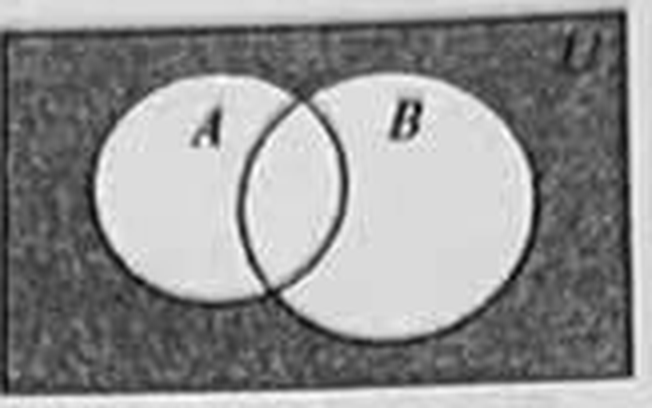
\includegraphics[width=0.30\textwidth]{figures/venn_AB_complement.png}
\end{center}

\ans{$\overline{A\cup B}$}

\ifanswer
\solbegin
\step{图中阴影部分在集合 $A$、$B$ 的外部，即在全集 $U$ 中但不属于 $A$、也不属于 $B$.}
\step{这正是 $A\cup B$ 在全集 $U$ 中的补集，故可表示为 $\overline{A\cup B}$（即 $\complement_U(A\cup B)$）.}
\solend

\fi

\item 设全集 $U=\R$，集合 $A=\{x\mid 2\leqslant x<5\}$，$B=\{x\mid 3<x<6\}$，则 $\overline{A}\cap B=$ \blankline[4.4em]（用区间表示）.

\ans{$[5,6)$}

\ifanswer
\solbegin
\step{在全集 $\R$ 中，$\overline{A}=(-\infty,2)\cup[5,+\infty)$.}
\step{又 $B=(3,6)$，取两集合的公共部分得 $\overline{A}\cap B=[5,6)$.}
\solend

\fi

\item 用反证法证明“$a,b\in\N$，$ab$ 可被 5 整除，那么 $a,b$ 中至少有一个能被 5 整除”时应假设 \blankline[4.4em].

\ans{$a,b$ 都不能被 5 整除}

\ifanswer
\solbegin
\step{反证法需假设结论的反面成立.}
\step{“$a,b$ 中至少有一个能被 5 整除”的反面是“$a,b$ 中没有一个能被 5 整除”，即 $a,b$ 都不能被 5 整除.}
\solend

\fi

\item 满足 $M\subseteq\{a_1,a_2,a_3,a_4,a_5\}$，且 $M\cap\{a_1,a_2,a_3\}=\{a_1,a_2\}$，则集合 $M$ 的个数是 \blankline[2.4em].

\ans{$4$}

\ifanswer
\solbegin
\step{由 $M\cap\{a_1,a_2,a_3\}=\{a_1,a_2\}$ 得 $a_1\in M$，$a_2\in M$，$a_3\notin M$.}
\step{又 $M\subseteq\{a_1,a_2,a_3,a_4,a_5\}$，所以 $a_4$、$a_5$ 可以属于 $M$，也可以不属于 $M$.}
\step{即 $M=\{a_1,a_2\}\cup S$，其中 $S\subseteq\{a_4,a_5\}$，共有 $2^2=4$ 个.}
\solend

\fi

\item 已知集合 $A=\{(x,y)\mid y=x^2\}$，$B=\left\{(x,y)\mid \dfrac{y-1}{x-1}=\dfrac{1}{2}\right\}$，则 $A\cap B=$ \blankline[5.2em].

\ans{$\left\{\left(-\dfrac{1}{2},\dfrac{1}{4}\right)\right\}$}

\ifanswer
\solbegin
\step{集合 $B$ 中的点满足 $y=\dfrac{1}{2}x+\dfrac{1}{2}$，且 $x\neq 1$.}
\step{代入 $y=x^2$ 得 $2x^2-x-1=0$，解得 $x=1$ 或 $x=-\dfrac{1}{2}$.}
\step{因为 $x\neq 1$，所以 $x=-\dfrac{1}{2}$，此时 $y=\dfrac{1}{4}$.}
\step{所以 $A\cap B=\left\{\left(-\dfrac{1}{2},\dfrac{1}{4}\right)\right\}$.}
\solend

\fi

\item 已知集合 $\{a,b,c\}=\{0,1,2\}$，且下列三个关系：①$a\neq 2$ ②$b=2$ ③$c\neq 0$ 有且只有一个正确，则 $100a+10b+c$ 等于 \blankline[2.4em].

\ans{$201$}

\ifanswer
\solbegin
\step{$a,b,c$ 是 $0,1,2$ 的一个排列，共 6 种情形，逐一检验三个关系的真假：}
\step{$(a,b,c)=(0,1,2)$：①真、②假、③真，两个正确，不合；$(0,2,1)$：三个都真，不合；}
\step{$(1,0,2)$：①真、②假、③真，两个正确，不合；$(1,2,0)$：①真、②真、③假，两个正确，不合；}
\step{$(2,0,1)$：①假、②假、③真，恰有一个正确，符合；$(2,1,0)$：三个都假，不合.}
\step{所以 $(a,b,c)=(2,0,1)$，$100a+10b+c=200+0+1=201$.}
\solend

\fi

\item “$x_1>3$ 且 $x_2>3$”是“$x_1+x_2>6$ 且 $x_1x_2>9$”的 \blankline[4.4em] 条件.（选填“充分非必要”，“必要非充分”，“充要”，“既非充分也非必要”）

\ans{充分非必要}

\ifanswer
\solbegin
\step{充分性：若 $x_1>3$ 且 $x_2>3$，则 $x_1+x_2>6$，且 $x_1x_2>9$，故充分性成立.}
\step{必要性：取 $x_1=2$、$x_2=5$，有 $x_1+x_2=7>6$、$x_1x_2=10>9$，但 $x_1>3$ 不成立，故必要性不成立.}
\step{所以应填“充分非必要”.}
\solend

\fi

% 注：第 11 题系 2010 年上海高考理科第 14 题的改写（原题要求选出 4 个子集，官方答案 36）。
%     原题官方解答明言「A、B 可以互换，即视为一种选法」，即**不计先后**计数；
%     按此口径本改写题的答案为 5。（原卷学生作答为 10，是把 A⊆B 与 B⊆A 重复计入。）
\item 在集合 $U=\{a,b,c,d\}$ 的子集中选出 2 个不同的子集，需同时满足以下两个条件：(1)$a,b$ 都要选出 (2)对选出的任意两个子集 $A$ 和 $B$，必有 $A\subseteq B$ 或 $B\subseteq A$，那么共有 \blankline[2.4em] 种不同的选法.

\ans{$5$}

\ifanswer
\solbegin
\step{由 (1) 知 $a,b$ 都要选出，即 $a,b$ 都属于所选的两个子集；由 (2) 知所选的两个子集必须可比.}
\step{含 $a,b$ 的子集只有 $\{a,b\}$、$\{a,b,c\}$、$\{a,b,d\}$、$\{a,b,c,d\}$ 共 4 个.}
\step{在这 4 个子集中取出两个不同的且可比的（一个包含另一个），只有下列 5 组：}
\step{$\{a,b\}\subset\{a,b,c\}$、$\{a,b\}\subset\{a,b,d\}$、$\{a,b\}\subset\{a,b,c,d\}$、$\{a,b,c\}\subset\{a,b,c,d\}$、$\{a,b,d\}\subset\{a,b,c,d\}$.}
\step{注意「选出 2 个子集」的选法\textbf{不计先后}：把这两个子集分别叫作 $A$、$B$ 只是给它们取个名字，$A\subseteq B$ 与 $B\subseteq A$ 说的是同一组子集，算同一种选法.}
\step{（本题由 2010 年上海高考理科第 14 题改写，原题要求选出 4 个子集，其官方答案 36 正是按「$A$、$B$ 可以互换，即视为一种选法」的不计先后口径计数.）}
\step{所以共有 5 种不同的选法.}
\solend

\fi

\end{enumerate}

\bigsec{二、选择题}

\begin{enumerate}
\setcounter{enumi}{11}

\item 已知 $M=(-\infty,\sqrt{3}]$，$a=\sqrt{3}$，则下列关系中正确的是（\quad）.

A. $a\subset M$\qquad B. $a\in M$\qquad C. $\{a\}\in M$\qquad D. $M\subset\{a\}$

\ans{B}

\ifanswer
\solbegin
\step{因为 $\sqrt{3}\leqslant\sqrt{3}$，所以 $a=\sqrt{3}\in M$，B 正确.}
\step{$a$ 是元素、$M$ 是集合，元素与集合之间用 $\in$ 表示，不能用 $\subset$，故 A、D 错误；}
\step{$\{a\}$ 是集合，集合与集合之间应是包含关系（且 $\{a\}\subseteq M$），不能用 $\in$，故 C 错误.}
\step{故选 B.}
\solend

\fi

% 注：原卷此处印作“已知集合{(x,y)|x^2+y^2≤3, x∈Z, y∈Z}”，集合未记作 A，
%     却设问“则 A 中的元素个数是”，显系漏排“A=”；本稿补上，其余照原卷。
\item 已知集合 $A=\{(x,y)\mid x^2+y^2\leqslant 3,\ x\in\Z,\ y\in\Z\}$，则 $A$ 中的元素个数是（\quad）.

A. $9$\qquad B. $8$\qquad C. $5$\qquad D. $4$

\ans{A}

\ifanswer
\solbegin
\step{逐一列举：$x=0$ 时 $y^2\leqslant 3$，$y=-1,0,1$，得 $(0,-1),(0,0),(0,1)$，共 3 个；}
\step{$x=\pm 1$ 时 $y^2\leqslant 2$，$y=-1,0,1$，各得 3 个，共 6 个（$x^2+y^2=2\leqslant 3$ 满足条件）；}
\step{$|x|\geqslant 2$ 时 $x^2\geqslant 4>3$，无解.}
\step{所以 $A$ 中元素个数为 $3+6=9$. 故选 A.}
\solend

\fi

\item 集合 $A=\{x\mid x=(2k-1)\pi,\ k\in\Z\}$ 与 $B=\{x\mid x=(4n\pm 1)\pi,\ n\in\Z\}$ 之间的关系是（\quad）.

A. $A\subset B$\qquad B. $B\subset A$\qquad C. $A=B$\qquad D. 不确定

\ans{C}

\ifanswer
\solbegin
\step{$A$ 由 $\pi$ 的一切奇数倍组成，即 $A=\{\cdots,-3\pi,-\pi,\pi,3\pi,\cdots\}$.}
\step{$B$ 中 $4n+1$ 与 $4n-1$ （$n\in\Z$）都是奇数，故 $B\subseteq A$；}
\step{反之，任一奇数除以 4 的余数只能是 1 或 3：形如 $4m+1$ 的奇数含于 $B$（取 $n=m$），形如 $4m+3=4(m+1)-1$ 的奇数也含于 $B$（取 $n=m+1$），所以 $A\subseteq B$.}
\step{于是 $A\subseteq B$ 且 $B\subseteq A$，即 $A=B$. 故选 C.}
\solend

\fi

\item 设 $T$ 是由正三角形 $P_1P_2P_3$ 边上及其内部的点构成的集合，点 $O$ 是 $\triangle P_1P_2P_3$ 的中心. 若集合 $S=\{P\mid P\in T,\ |PO|\leqslant|PO_i|,\ i=1,2,3\}$，（符号 $|AB|$ 表示平面上两点 $A,B$ 间的距离），则集合 $S$ 表示的平面区域是（\quad）.

A. 四边形区域；\qquad B. 三角形区域；\qquad C. 六边形区域；\qquad D. 五边形区域；

\ans{C}

\ifanswer
\solbegin
\step{$|PO|\leqslant|PO_i|$ 表示点 $P$ 到 $O$ 的距离不大于到顶点 $P_i$ 的距离，即 $P$ 落在线段 $OP_i$ 的垂直平分线靠 $O$ 的那一侧（含该线）.}
\step{对 $i=1,2,3$ 各有一条这样的直线，它们分别把三角形靠近 $P_1$、$P_2$、$P_3$ 的一个小角（三角形）截掉；}
\step{逐一直观验证可知这三条直线两两的交点都在三角形内部，三个角互不重叠，截去三个角后剩下的区域共有 6 条边.}
\step{所以集合 $S$ 表示的平面区域是六边形区域. 故选 C.}
\solend

\fi

\end{enumerate}

\bigsec{三、解答题}

\begin{enumerate}
\setcounter{enumi}{15}

\item（10 分，第 1 小问 5 分，第 2 小问 5 分）已知集合 $A=\{x\mid a\leqslant x\leqslant a+2\}$，集合 $B=\{x\mid x<-1\text{ 或 }x>5\}$，全集 $U=\R$.

\begin{enumerate}[label=(\arabic*)]
\item 若 $a=1$，求 $\overline{A}\cup B$；
\item 若 $A\subseteq B$，求实数 $a$ 的取值范围.
\end{enumerate}

\ans{（1）$(-\infty,1)\cup(3,+\infty)$；（2）$(-\infty,-3)\cup(5,+\infty)$}

\ifanswer
\solbegin
\stepm{(1)}{$a=1$ 时 $A=\{x\mid 1\leqslant x\leqslant 3\}=[1,3]$，则 $\overline{A}=(-\infty,1)\cup(3,+\infty)$.}
\step{又 $B=(-\infty,-1)\cup(5,+\infty)$，而 $B\subseteq\overline{A}$（因 $5>3$、$-1<1$），}
\step{所以 $\overline{A}\cup B=(-\infty,1)\cup(3,+\infty)$.}
\stepm{(2)}{因为 $a\leqslant a+2$，所以集合 $A=\{x\mid a\leqslant x\leqslant a+2\}$ 始终非空.}
\step{要使 $A\subseteq B$，只需 $A$ 与 $[-1,5]$ 没有公共点，即 $a+2<-1$ 或 $a>5$.}
\step{解得 $a<-3$ 或 $a>5$，所以实数 $a$ 的取值范围是 $(-\infty,-3)\cup(5,+\infty)$.}
\solend

\fi

\ansspace[10]

\item（10 分，第 1 小问 5 分，第 2 小问 5 分）已知 $A=\{x\mid x^2+x-2=0\}$，$B=\{x\mid x^2+ax+2a-4=0\}$.

\begin{enumerate}[label=(\arabic*)]
\item 若 $A=B$，求实数 $a$ 的值；
\item 若 $B\subseteq A$，求实数 $a$ 的值.
\end{enumerate}

\ans{（1）$a=1$；（2）$a=1$ 或 $a=4$}

\ifanswer
\solbegin
\stepm{(1)}{由 $x^2+x-2=0$ 解得 $x=1$ 或 $x=-2$，所以 $A=\{1,-2\}$.}
\step{由 $A=B$ 知 $1$、$-2$ 是方程 $x^2+ax+2a-4=0$ 的两根，由根与系数的关系得 $1+(-2)=-a$，所以 $a=1$；}
\step{此时 $2a-4=-2=1\times(-2)$，与两根之积相符，故 $a=1$.}
\stepm{(2)}{方程 $x^2+ax+2a-4=0$ 的判别式 $\Delta=a^2-4(2a-4)=(a-4)^2\geqslant 0$ 恒成立，所以集合 $B$ 不可能是空集.}
\step{由 $B\subseteq A$ 知 $B=\{1\}$ 或 $B=\{-2\}$ 或 $B=\{1,-2\}$.}
\step{若 $B=\{1\}$，则 $1$ 是二重根，$1+1=-a$ 且 $1\times 1=2a-4$，即 $a=-2$ 且 $a=\dfrac{5}{2}$，无解；}
\step{若 $B=\{-2\}$，则 $-2$ 是二重根，$(-2)+(-2)=-a$ 且 $(-2)\times(-2)=2a-4$，两式都给出 $a=4$，符合；}
\step{若 $B=\{1,-2\}$，则 $1+(-2)=-a$，得 $a=1$，此时 $2a-4=-2=1\times(-2)$，符合.}
\step{综上，$a=1$ 或 $a=4$.}
\solend

\fi

\ansspace[12]

\item（11 分，第 1 小问 3 分，第 2 小问 3 分，第 3 小问 5 分）已知非空数集 $S$ 满足：对任意给定的 $x,y\in S$（$x,y$ 可以相同），有 $x+y\in S$ 且 $x-y\in S$.

\begin{enumerate}[label=(\arabic*)]
\item 哪个数一定是 $S$ 中的元素?说明理由；
\item 若 $S$ 是有限集，求 $S$；
\item 若 $S$ 中最小的正数为 5，求 $S$.
\end{enumerate}

\ans{（1）$0$；（2）$S=\{0\}$；（3）$S=\{x\mid x=5a,\ a\in\Z\}$}

\ifanswer
\solbegin
\stepm{(1)}{$0$ 一定是 $S$ 中的元素. 理由：$S$ 非空，取 $x\in S$，在 $x-y\in S$ 中令 $y=x$（$x,y$ 可以相同），得 $x-x=0\in S$.}
\stepm{(2)}{若 $S$ 是有限集，则 $S=\{0\}$. 理由：取 $x\in S$ 且 $x\neq 0$，由 $x+y\in S$ 依次得 $2x=x+x\in S$，$3x=2x+x\in S$，$\cdots$，即 $kx\in S$（$k=1,2,3,\cdots$）；}
\step{这些数互不相同，与 $S$ 是有限集矛盾，所以 $S$ 中除 $0$ 外没有别的元素，即 $S=\{0\}$（此时 $0+0=0\in S$，$0-0=0\in S$，符合条件）.}
\stepm{(3)}{因为 $5\in S$，由 $x+y\in S$ 得 $5+5=10\in S$，$10+5=15\in S$，$\cdots$，故一切正整数倍的 $5$ 都在 $S$ 中；}
\step{又由 $x-y\in S$ 得 $5-5=0\in S$，$0-5=-5\in S$，$-5-5=-10\in S$，$\cdots$，故一切负整数倍的 $5$ 也都在 $S$ 中，即 $\{5a\mid a\in\Z\}\subseteq S$.}
\step{反之，任取 $s\in S$，由 $5\in S$ 及封闭性知 $s-5k\in S$（$k\in\Z$）；把 $s$ 写成 $s=5q+r$（$q\in\Z$，$0\leqslant r<5$），取 $k=q$ 得 $r=s-5q\in S$.}
\step{若 $r>0$，则 $S$ 中有比 $5$ 更小的正数 $r$，与“$S$ 中最小的正数为 5”矛盾，故只能 $r=0$，即 $s=5q$.}
\step{所以 $S=\{x\mid x=5a,\ a\in\Z\}$.}
\solend

\fi

\ansspace[12]

\end{enumerate}

\bigsec{附加题}

\begin{enumerate}
\setcounter{enumi}{18}

\item 已知集合 $A,B,C\subseteq\{1,2,3,\cdots,2024\}$，且 $A\subseteq B\subseteq C$，则有序集合组 $(A,B,C)$ 的个数是 \blankline[3.2em].

\ans{$4^{2024}$}

\ifanswer
\solbegin
\step{对 $U=\{1,2,\cdots,2024\}$ 中的每个元素，它与 $A,B,C$ 的关系只有四种可能：}
\step{在 $A,B,C$ 中都出现；不在 $A$ 中而在 $B,C$ 中出现；只在 $C$ 中出现；在三个集合中都不出现.}
\step{反过来，任取每个元素的一种归属方式，都恰好得到一个满足 $A\subseteq B\subseteq C$ 的有序集合组，故不同的组与不同的归属方式一一对应.}
\step{所以共有 $4\times 4\times\cdots\times 4=4^{2024}$ 个有序集合组.}
\solend

\fi

\item 已知集合 $M=\{1,2,\cdots,10\}$，对它的非空子集 $A$，将 $A$ 中的每个元素 $k$ 都乘以 $(-1)^k$ 再求和，如 $A=\{2,3,6\}$，可求得和为 $(-1)^2\times 2+(-1)^3\times 3+(-1)^6\times 6=5$. 试对 $M$ 的所有非空子集，求这些和的总和 \blankline[3.2em].

\ans{$2560$}

\ifanswer
\solbegin
\step{元素 $k$（$k=1,2,\cdots,10$）出现在 $M$ 的 $2^{9}$ 个非空子集中（其余 9 个元素任取）.}
\step{所以在所有非空子集的和中，$k$ 贡献的总量为 $2^{9}\times(-1)^k\cdot k=512\times(-1)^kk$.}
\step{于是这些和的总和为 $512\displaystyle\sum_{k=1}^{10}(-1)^kk=512\times(-1+2-3+4-5+6-7+8-9+10)=512\times 5=2560$.}
\solend

\fi

\item 设 $a_1,a_2,a_3,a_4$ 是 4 个有理数，使得 $\{a_ia_j\mid 1\leqslant i<j\leqslant 4\}=\left\{-24,-2,-\dfrac{3}{2},-\dfrac{1}{8},1,3\right\}$. 求 $a_1+a_2+a_3+a_4=$ \blankline[3.2em].

\ans{$\pm\dfrac{9}{4}$（两组解，和分别为 $-\dfrac{9}{4}$ 与 $\dfrac{9}{4}$）}

\ifanswer
\solbegin
\step{六个乘积中有 4 个负数、2 个正数. 设 4 个数中正数有 $p$ 个、负数有 $q$ 个（$p+q=4$），则异号的两数相乘得负数，其个数为 $pq$；由 $pq=4$ 得 $p=q=2$，即恰有 2 个正数、2 个负数.}
\step{把 4 个数的绝对值记作 $w,x,y,z>0$，则六个两两乘积的绝对值为 $24,2,\dfrac{3}{2},\dfrac{1}{8},1,3$；其中 $1$ 与 $3$ 来自两对同号的数，$24,2,\dfrac{3}{2},\dfrac{1}{8}$ 来自四对异号的数.}
\step{由 $(a_1a_2a_3a_4)^3=(-24)\times(-2)\times\left(-\dfrac{3}{2}\right)\times\left(-\dfrac{1}{8}\right)\times 1\times 3=27$ 得 $a_1a_2a_3a_4=3$，即去符号后 $wxyz=3$.}
\step{逐一检验可知 $w,x,y,z$ 只能是 $\left\{4,\dfrac{1}{4},6,\dfrac{1}{2}\right\}$：其中 $4\times\dfrac{1}{4}=1$、$6\times\dfrac{1}{2}=3$ 为同号两对的乘积，$4\times 6=24$、$4\times\dfrac{1}{2}=2$、$\dfrac{1}{4}\times 6=\dfrac{3}{2}$、$\dfrac{1}{4}\times\dfrac{1}{2}=\dfrac{1}{8}$ 为异号四对的乘积.}
\step{于是 $\left\{4,\dfrac{1}{4}\right\}$ 中的两个数同号、$\left\{6,\dfrac{1}{2}\right\}$ 中的两个数同号，且这两组异号，得两组解：}
\step{$4,\ \dfrac{1}{4},\ -6,\ -\dfrac{1}{2}$，和为 $-\dfrac{9}{4}$；\quad 或 \quad $6,\ \dfrac{1}{2},\ -4,\ -\dfrac{1}{4}$，和为 $\dfrac{9}{4}$.}
\step{两组解的六个乘积都恰为 $-24,-2,-\dfrac{3}{2},-\dfrac{1}{8},1,3$，与原卷所给集合相同.}
\step{所以 $a_1+a_2+a_3+a_4=\pm\dfrac{9}{4}$.}
\solend

\fi

\end{enumerate}

\end{document}
"
%
% 原始材料为学生作业的手机翻拍照片（卷面为学生本人的**手写作答**，未见教师批改痕迹）。
% 试题文字照原卷录入；答案版给出的是**经核验的正确解答与解析**，与原卷手写答案的差异见 README。
%
% 与原卷的两处排版差异（均已在 README「说明」中交代）：
%   ① 原卷未印分节标题与分值，本稿按题型补「一、填空题 / 二、选择题 / 三、解答题」三节
%      （「附加题」原卷有印）；
%   ② 第 13 题原卷印作「已知集合{(x,y)|…}」，集合未记作 A 却被设问为「A 中的元素个数」，
%      显系漏排「A=」，本稿补上。

% 本篇的正文与家长拍照卷 `高一b_大同中学_第二周周末练习1（补）` **完全相同**——同一份作业，
% 试卷版/答案版也都是同一份源码编译而来；`高一b` 的 4 张原图另存于
% `原图/高一b_大同中学_第二周周末练习1（补）/`，本卷 `原图/` 下是同一组照片的副本。
% 经核对，这份作业就是公众号「魔都数学加油站」连载「27学年高一16——2026-2027年上海市大同中学
% 高一上周末作业2.1」的那一份：**题号与题干逐题一致**，只是公众号版略去了填空第 1、2 题，
% 故拍照卷反而是更完整的版本（对照关系见 README「与公众号连载号的对照表」）。
%
% 本卷的编号与连载号对齐（高一16），卷面标题因此**不带**「（补）」；标题里的「大同中学」为**本稿所加**
% （原卷标题只有作业名，校名只印在页眉「上海市大同…」）。带「（补）」的 `高一b` 保留为
% 拍照原件的转录本，两者内容一字不差。
%
% 一处与公众号讲评版的差异需留意：本卷第 11 题的答案按 2010 年上海高考理科第 14 题官方解答
% 「A、B 可以互换，即视为一种选法」的不计先后口径取 5，而公众号讲评版把它按有先后的 32 计数
% （该题学生原作答为 10）。取舍理由见该题下的 `%` 注。
\documentclass[a4paper,11pt]{article}
\usepackage{common}

\begin{document}

\examtitlest[3]{2026--2027 学年度大同中学高一上数学第二周周末练习1}{集合与常用逻辑用语}

\bigsec{一、填空题}

\begin{enumerate}

\item 用列举法表示集合 $\{x\mid -2<x\leqslant 2,\ x\in\Z\}=$ \blankline[2.4em].

\ans{$\{-1,0,1,2\}$}

\ifanswer
\solbegin
\step{集合中的元素是满足 $-2<x\leqslant 2$ 的整数，即 $-1$、$0$、$1$、$2$.}
\step{所以用列举法表示为 $\{-1,0,1,2\}$.}
\solend

\fi

\item 设集合 $A=\{1,a\}$，$B=\{1,a^2\}$，若 $A=B$，则实数 $a$ 的值为 \blankline[2.4em].

\ans{$a=0$}

\ifanswer
\solbegin
\step{由 $A=B$ 得 $a^2=a$，解得 $a=0$ 或 $a=1$.}
\step{当 $a=1$ 时，$A=\{1,1\}$，不符合集合元素的互异性，舍去；}
\step{当 $a=0$ 时，$A=\{1,0\}$，$B=\{1,0\}$，两集合相等，符合条件.}
\step{所以 $a=0$.}
\solend

\fi

\item 已知集合 $A=\{0,2,3,4,5\}$，$B=\{2,3,5,7\}$，$C=\{2,3,6\}$，则 $(A\cap B)\cup C=$ \blankline[4.4em].

\ans{$\{2,3,5,6\}$}

\ifanswer
\solbegin
\step{$A\cap B=\{0,2,3,4,5\}\cap\{2,3,5,7\}=\{2,3,5\}$.}
\step{所以 $(A\cap B)\cup C=\{2,3,5\}\cup\{2,3,6\}=\{2,3,5,6\}$.}
\solend

\fi

\item 设全集为 $U$，用集合 $A,B$ 的交、并或补集符号表示图中的阴影部分是 \blankline[4.4em].

\begin{center}
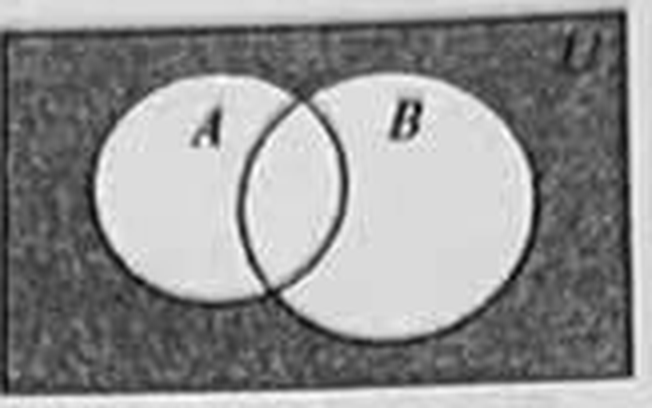
\includegraphics[width=0.30\textwidth]{figures/venn_AB_complement.png}
\end{center}

\ans{$\overline{A\cup B}$}

\ifanswer
\solbegin
\step{图中阴影部分在集合 $A$、$B$ 的外部，即在全集 $U$ 中但不属于 $A$、也不属于 $B$.}
\step{这正是 $A\cup B$ 在全集 $U$ 中的补集，故可表示为 $\overline{A\cup B}$（即 $\complement_U(A\cup B)$）.}
\solend

\fi

\item 设全集 $U=\R$，集合 $A=\{x\mid 2\leqslant x<5\}$，$B=\{x\mid 3<x<6\}$，则 $\overline{A}\cap B=$ \blankline[4.4em]（用区间表示）.

\ans{$[5,6)$}

\ifanswer
\solbegin
\step{在全集 $\R$ 中，$\overline{A}=(-\infty,2)\cup[5,+\infty)$.}
\step{又 $B=(3,6)$，取两集合的公共部分得 $\overline{A}\cap B=[5,6)$.}
\solend

\fi

\item 用反证法证明“$a,b\in\N$，$ab$ 可被 5 整除，那么 $a,b$ 中至少有一个能被 5 整除”时应假设 \blankline[4.4em].

\ans{$a,b$ 都不能被 5 整除}

\ifanswer
\solbegin
\step{反证法需假设结论的反面成立.}
\step{“$a,b$ 中至少有一个能被 5 整除”的反面是“$a,b$ 中没有一个能被 5 整除”，即 $a,b$ 都不能被 5 整除.}
\solend

\fi

\item 满足 $M\subseteq\{a_1,a_2,a_3,a_4,a_5\}$，且 $M\cap\{a_1,a_2,a_3\}=\{a_1,a_2\}$，则集合 $M$ 的个数是 \blankline[2.4em].

\ans{$4$}

\ifanswer
\solbegin
\step{由 $M\cap\{a_1,a_2,a_3\}=\{a_1,a_2\}$ 得 $a_1\in M$，$a_2\in M$，$a_3\notin M$.}
\step{又 $M\subseteq\{a_1,a_2,a_3,a_4,a_5\}$，所以 $a_4$、$a_5$ 可以属于 $M$，也可以不属于 $M$.}
\step{即 $M=\{a_1,a_2\}\cup S$，其中 $S\subseteq\{a_4,a_5\}$，共有 $2^2=4$ 个.}
\solend

\fi

\item 已知集合 $A=\{(x,y)\mid y=x^2\}$，$B=\left\{(x,y)\mid \dfrac{y-1}{x-1}=\dfrac{1}{2}\right\}$，则 $A\cap B=$ \blankline[5.2em].

\ans{$\left\{\left(-\dfrac{1}{2},\dfrac{1}{4}\right)\right\}$}

\ifanswer
\solbegin
\step{集合 $B$ 中的点满足 $y=\dfrac{1}{2}x+\dfrac{1}{2}$，且 $x\neq 1$.}
\step{代入 $y=x^2$ 得 $2x^2-x-1=0$，解得 $x=1$ 或 $x=-\dfrac{1}{2}$.}
\step{因为 $x\neq 1$，所以 $x=-\dfrac{1}{2}$，此时 $y=\dfrac{1}{4}$.}
\step{所以 $A\cap B=\left\{\left(-\dfrac{1}{2},\dfrac{1}{4}\right)\right\}$.}
\solend

\fi

\item 已知集合 $\{a,b,c\}=\{0,1,2\}$，且下列三个关系：①$a\neq 2$ ②$b=2$ ③$c\neq 0$ 有且只有一个正确，则 $100a+10b+c$ 等于 \blankline[2.4em].

\ans{$201$}

\ifanswer
\solbegin
\step{$a,b,c$ 是 $0,1,2$ 的一个排列，共 6 种情形，逐一检验三个关系的真假：}
\step{$(a,b,c)=(0,1,2)$：①真、②假、③真，两个正确，不合；$(0,2,1)$：三个都真，不合；}
\step{$(1,0,2)$：①真、②假、③真，两个正确，不合；$(1,2,0)$：①真、②真、③假，两个正确，不合；}
\step{$(2,0,1)$：①假、②假、③真，恰有一个正确，符合；$(2,1,0)$：三个都假，不合.}
\step{所以 $(a,b,c)=(2,0,1)$，$100a+10b+c=200+0+1=201$.}
\solend

\fi

\item “$x_1>3$ 且 $x_2>3$”是“$x_1+x_2>6$ 且 $x_1x_2>9$”的 \blankline[4.4em] 条件.（选填“充分非必要”，“必要非充分”，“充要”，“既非充分也非必要”）

\ans{充分非必要}

\ifanswer
\solbegin
\step{充分性：若 $x_1>3$ 且 $x_2>3$，则 $x_1+x_2>6$，且 $x_1x_2>9$，故充分性成立.}
\step{必要性：取 $x_1=2$、$x_2=5$，有 $x_1+x_2=7>6$、$x_1x_2=10>9$，但 $x_1>3$ 不成立，故必要性不成立.}
\step{所以应填“充分非必要”.}
\solend

\fi

% 注：第 11 题系 2010 年上海高考理科第 14 题的改写（原题要求选出 4 个子集，官方答案 36）。
%     原题官方解答明言「A、B 可以互换，即视为一种选法」，即**不计先后**计数；
%     按此口径本改写题的答案为 5。（原卷学生作答为 10，是把 A⊆B 与 B⊆A 重复计入。）
\item 在集合 $U=\{a,b,c,d\}$ 的子集中选出 2 个不同的子集，需同时满足以下两个条件：(1)$a,b$ 都要选出 (2)对选出的任意两个子集 $A$ 和 $B$，必有 $A\subseteq B$ 或 $B\subseteq A$，那么共有 \blankline[2.4em] 种不同的选法.

\ans{$5$}

\ifanswer
\solbegin
\step{由 (1) 知 $a,b$ 都要选出，即 $a,b$ 都属于所选的两个子集；由 (2) 知所选的两个子集必须可比.}
\step{含 $a,b$ 的子集只有 $\{a,b\}$、$\{a,b,c\}$、$\{a,b,d\}$、$\{a,b,c,d\}$ 共 4 个.}
\step{在这 4 个子集中取出两个不同的且可比的（一个包含另一个），只有下列 5 组：}
\step{$\{a,b\}\subset\{a,b,c\}$、$\{a,b\}\subset\{a,b,d\}$、$\{a,b\}\subset\{a,b,c,d\}$、$\{a,b,c\}\subset\{a,b,c,d\}$、$\{a,b,d\}\subset\{a,b,c,d\}$.}
\step{注意「选出 2 个子集」的选法\textbf{不计先后}：把这两个子集分别叫作 $A$、$B$ 只是给它们取个名字，$A\subseteq B$ 与 $B\subseteq A$ 说的是同一组子集，算同一种选法.}
\step{（本题由 2010 年上海高考理科第 14 题改写，原题要求选出 4 个子集，其官方答案 36 正是按「$A$、$B$ 可以互换，即视为一种选法」的不计先后口径计数.）}
\step{所以共有 5 种不同的选法.}
\solend

\fi

\end{enumerate}

\bigsec{二、选择题}

\begin{enumerate}
\setcounter{enumi}{11}

\item 已知 $M=(-\infty,\sqrt{3}]$，$a=\sqrt{3}$，则下列关系中正确的是（\quad）.

A. $a\subset M$\qquad B. $a\in M$\qquad C. $\{a\}\in M$\qquad D. $M\subset\{a\}$

\ans{B}

\ifanswer
\solbegin
\step{因为 $\sqrt{3}\leqslant\sqrt{3}$，所以 $a=\sqrt{3}\in M$，B 正确.}
\step{$a$ 是元素、$M$ 是集合，元素与集合之间用 $\in$ 表示，不能用 $\subset$，故 A、D 错误；}
\step{$\{a\}$ 是集合，集合与集合之间应是包含关系（且 $\{a\}\subseteq M$），不能用 $\in$，故 C 错误.}
\step{故选 B.}
\solend

\fi

% 注：原卷此处印作“已知集合{(x,y)|x^2+y^2≤3, x∈Z, y∈Z}”，集合未记作 A，
%     却设问“则 A 中的元素个数是”，显系漏排“A=”；本稿补上，其余照原卷。
\item 已知集合 $A=\{(x,y)\mid x^2+y^2\leqslant 3,\ x\in\Z,\ y\in\Z\}$，则 $A$ 中的元素个数是（\quad）.

A. $9$\qquad B. $8$\qquad C. $5$\qquad D. $4$

\ans{A}

\ifanswer
\solbegin
\step{逐一列举：$x=0$ 时 $y^2\leqslant 3$，$y=-1,0,1$，得 $(0,-1),(0,0),(0,1)$，共 3 个；}
\step{$x=\pm 1$ 时 $y^2\leqslant 2$，$y=-1,0,1$，各得 3 个，共 6 个（$x^2+y^2=2\leqslant 3$ 满足条件）；}
\step{$|x|\geqslant 2$ 时 $x^2\geqslant 4>3$，无解.}
\step{所以 $A$ 中元素个数为 $3+6=9$. 故选 A.}
\solend

\fi

\item 集合 $A=\{x\mid x=(2k-1)\pi,\ k\in\Z\}$ 与 $B=\{x\mid x=(4n\pm 1)\pi,\ n\in\Z\}$ 之间的关系是（\quad）.

A. $A\subset B$\qquad B. $B\subset A$\qquad C. $A=B$\qquad D. 不确定

\ans{C}

\ifanswer
\solbegin
\step{$A$ 由 $\pi$ 的一切奇数倍组成，即 $A=\{\cdots,-3\pi,-\pi,\pi,3\pi,\cdots\}$.}
\step{$B$ 中 $4n+1$ 与 $4n-1$ （$n\in\Z$）都是奇数，故 $B\subseteq A$；}
\step{反之，任一奇数除以 4 的余数只能是 1 或 3：形如 $4m+1$ 的奇数含于 $B$（取 $n=m$），形如 $4m+3=4(m+1)-1$ 的奇数也含于 $B$（取 $n=m+1$），所以 $A\subseteq B$.}
\step{于是 $A\subseteq B$ 且 $B\subseteq A$，即 $A=B$. 故选 C.}
\solend

\fi

\item 设 $T$ 是由正三角形 $P_1P_2P_3$ 边上及其内部的点构成的集合，点 $O$ 是 $\triangle P_1P_2P_3$ 的中心. 若集合 $S=\{P\mid P\in T,\ |PO|\leqslant|PO_i|,\ i=1,2,3\}$，（符号 $|AB|$ 表示平面上两点 $A,B$ 间的距离），则集合 $S$ 表示的平面区域是（\quad）.

A. 四边形区域；\qquad B. 三角形区域；\qquad C. 六边形区域；\qquad D. 五边形区域；

\ans{C}

\ifanswer
\solbegin
\step{$|PO|\leqslant|PO_i|$ 表示点 $P$ 到 $O$ 的距离不大于到顶点 $P_i$ 的距离，即 $P$ 落在线段 $OP_i$ 的垂直平分线靠 $O$ 的那一侧（含该线）.}
\step{对 $i=1,2,3$ 各有一条这样的直线，它们分别把三角形靠近 $P_1$、$P_2$、$P_3$ 的一个小角（三角形）截掉；}
\step{逐一直观验证可知这三条直线两两的交点都在三角形内部，三个角互不重叠，截去三个角后剩下的区域共有 6 条边.}
\step{所以集合 $S$ 表示的平面区域是六边形区域. 故选 C.}
\solend

\fi

\end{enumerate}

\bigsec{三、解答题}

\begin{enumerate}
\setcounter{enumi}{15}

\item（10 分，第 1 小问 5 分，第 2 小问 5 分）已知集合 $A=\{x\mid a\leqslant x\leqslant a+2\}$，集合 $B=\{x\mid x<-1\text{ 或 }x>5\}$，全集 $U=\R$.

\begin{enumerate}[label=(\arabic*)]
\item 若 $a=1$，求 $\overline{A}\cup B$；
\item 若 $A\subseteq B$，求实数 $a$ 的取值范围.
\end{enumerate}

\ans{（1）$(-\infty,1)\cup(3,+\infty)$；（2）$(-\infty,-3)\cup(5,+\infty)$}

\ifanswer
\solbegin
\stepm{(1)}{$a=1$ 时 $A=\{x\mid 1\leqslant x\leqslant 3\}=[1,3]$，则 $\overline{A}=(-\infty,1)\cup(3,+\infty)$.}
\step{又 $B=(-\infty,-1)\cup(5,+\infty)$，而 $B\subseteq\overline{A}$（因 $5>3$、$-1<1$），}
\step{所以 $\overline{A}\cup B=(-\infty,1)\cup(3,+\infty)$.}
\stepm{(2)}{因为 $a\leqslant a+2$，所以集合 $A=\{x\mid a\leqslant x\leqslant a+2\}$ 始终非空.}
\step{要使 $A\subseteq B$，只需 $A$ 与 $[-1,5]$ 没有公共点，即 $a+2<-1$ 或 $a>5$.}
\step{解得 $a<-3$ 或 $a>5$，所以实数 $a$ 的取值范围是 $(-\infty,-3)\cup(5,+\infty)$.}
\solend

\fi

\ansspace[10]

\item（10 分，第 1 小问 5 分，第 2 小问 5 分）已知 $A=\{x\mid x^2+x-2=0\}$，$B=\{x\mid x^2+ax+2a-4=0\}$.

\begin{enumerate}[label=(\arabic*)]
\item 若 $A=B$，求实数 $a$ 的值；
\item 若 $B\subseteq A$，求实数 $a$ 的值.
\end{enumerate}

\ans{（1）$a=1$；（2）$a=1$ 或 $a=4$}

\ifanswer
\solbegin
\stepm{(1)}{由 $x^2+x-2=0$ 解得 $x=1$ 或 $x=-2$，所以 $A=\{1,-2\}$.}
\step{由 $A=B$ 知 $1$、$-2$ 是方程 $x^2+ax+2a-4=0$ 的两根，由根与系数的关系得 $1+(-2)=-a$，所以 $a=1$；}
\step{此时 $2a-4=-2=1\times(-2)$，与两根之积相符，故 $a=1$.}
\stepm{(2)}{方程 $x^2+ax+2a-4=0$ 的判别式 $\Delta=a^2-4(2a-4)=(a-4)^2\geqslant 0$ 恒成立，所以集合 $B$ 不可能是空集.}
\step{由 $B\subseteq A$ 知 $B=\{1\}$ 或 $B=\{-2\}$ 或 $B=\{1,-2\}$.}
\step{若 $B=\{1\}$，则 $1$ 是二重根，$1+1=-a$ 且 $1\times 1=2a-4$，即 $a=-2$ 且 $a=\dfrac{5}{2}$，无解；}
\step{若 $B=\{-2\}$，则 $-2$ 是二重根，$(-2)+(-2)=-a$ 且 $(-2)\times(-2)=2a-4$，两式都给出 $a=4$，符合；}
\step{若 $B=\{1,-2\}$，则 $1+(-2)=-a$，得 $a=1$，此时 $2a-4=-2=1\times(-2)$，符合.}
\step{综上，$a=1$ 或 $a=4$.}
\solend

\fi

\ansspace[12]

\item（11 分，第 1 小问 3 分，第 2 小问 3 分，第 3 小问 5 分）已知非空数集 $S$ 满足：对任意给定的 $x,y\in S$（$x,y$ 可以相同），有 $x+y\in S$ 且 $x-y\in S$.

\begin{enumerate}[label=(\arabic*)]
\item 哪个数一定是 $S$ 中的元素?说明理由；
\item 若 $S$ 是有限集，求 $S$；
\item 若 $S$ 中最小的正数为 5，求 $S$.
\end{enumerate}

\ans{（1）$0$；（2）$S=\{0\}$；（3）$S=\{x\mid x=5a,\ a\in\Z\}$}

\ifanswer
\solbegin
\stepm{(1)}{$0$ 一定是 $S$ 中的元素. 理由：$S$ 非空，取 $x\in S$，在 $x-y\in S$ 中令 $y=x$（$x,y$ 可以相同），得 $x-x=0\in S$.}
\stepm{(2)}{若 $S$ 是有限集，则 $S=\{0\}$. 理由：取 $x\in S$ 且 $x\neq 0$，由 $x+y\in S$ 依次得 $2x=x+x\in S$，$3x=2x+x\in S$，$\cdots$，即 $kx\in S$（$k=1,2,3,\cdots$）；}
\step{这些数互不相同，与 $S$ 是有限集矛盾，所以 $S$ 中除 $0$ 外没有别的元素，即 $S=\{0\}$（此时 $0+0=0\in S$，$0-0=0\in S$，符合条件）.}
\stepm{(3)}{因为 $5\in S$，由 $x+y\in S$ 得 $5+5=10\in S$，$10+5=15\in S$，$\cdots$，故一切正整数倍的 $5$ 都在 $S$ 中；}
\step{又由 $x-y\in S$ 得 $5-5=0\in S$，$0-5=-5\in S$，$-5-5=-10\in S$，$\cdots$，故一切负整数倍的 $5$ 也都在 $S$ 中，即 $\{5a\mid a\in\Z\}\subseteq S$.}
\step{反之，任取 $s\in S$，由 $5\in S$ 及封闭性知 $s-5k\in S$（$k\in\Z$）；把 $s$ 写成 $s=5q+r$（$q\in\Z$，$0\leqslant r<5$），取 $k=q$ 得 $r=s-5q\in S$.}
\step{若 $r>0$，则 $S$ 中有比 $5$ 更小的正数 $r$，与“$S$ 中最小的正数为 5”矛盾，故只能 $r=0$，即 $s=5q$.}
\step{所以 $S=\{x\mid x=5a,\ a\in\Z\}$.}
\solend

\fi

\ansspace[12]

\end{enumerate}

\bigsec{附加题}

\begin{enumerate}
\setcounter{enumi}{18}

\item 已知集合 $A,B,C\subseteq\{1,2,3,\cdots,2024\}$，且 $A\subseteq B\subseteq C$，则有序集合组 $(A,B,C)$ 的个数是 \blankline[3.2em].

\ans{$4^{2024}$}

\ifanswer
\solbegin
\step{对 $U=\{1,2,\cdots,2024\}$ 中的每个元素，它与 $A,B,C$ 的关系只有四种可能：}
\step{在 $A,B,C$ 中都出现；不在 $A$ 中而在 $B,C$ 中出现；只在 $C$ 中出现；在三个集合中都不出现.}
\step{反过来，任取每个元素的一种归属方式，都恰好得到一个满足 $A\subseteq B\subseteq C$ 的有序集合组，故不同的组与不同的归属方式一一对应.}
\step{所以共有 $4\times 4\times\cdots\times 4=4^{2024}$ 个有序集合组.}
\solend

\fi

\item 已知集合 $M=\{1,2,\cdots,10\}$，对它的非空子集 $A$，将 $A$ 中的每个元素 $k$ 都乘以 $(-1)^k$ 再求和，如 $A=\{2,3,6\}$，可求得和为 $(-1)^2\times 2+(-1)^3\times 3+(-1)^6\times 6=5$. 试对 $M$ 的所有非空子集，求这些和的总和 \blankline[3.2em].

\ans{$2560$}

\ifanswer
\solbegin
\step{元素 $k$（$k=1,2,\cdots,10$）出现在 $M$ 的 $2^{9}$ 个非空子集中（其余 9 个元素任取）.}
\step{所以在所有非空子集的和中，$k$ 贡献的总量为 $2^{9}\times(-1)^k\cdot k=512\times(-1)^kk$.}
\step{于是这些和的总和为 $512\displaystyle\sum_{k=1}^{10}(-1)^kk=512\times(-1+2-3+4-5+6-7+8-9+10)=512\times 5=2560$.}
\solend

\fi

\item 设 $a_1,a_2,a_3,a_4$ 是 4 个有理数，使得 $\{a_ia_j\mid 1\leqslant i<j\leqslant 4\}=\left\{-24,-2,-\dfrac{3}{2},-\dfrac{1}{8},1,3\right\}$. 求 $a_1+a_2+a_3+a_4=$ \blankline[3.2em].

\ans{$\pm\dfrac{9}{4}$（两组解，和分别为 $-\dfrac{9}{4}$ 与 $\dfrac{9}{4}$）}

\ifanswer
\solbegin
\step{六个乘积中有 4 个负数、2 个正数. 设 4 个数中正数有 $p$ 个、负数有 $q$ 个（$p+q=4$），则异号的两数相乘得负数，其个数为 $pq$；由 $pq=4$ 得 $p=q=2$，即恰有 2 个正数、2 个负数.}
\step{把 4 个数的绝对值记作 $w,x,y,z>0$，则六个两两乘积的绝对值为 $24,2,\dfrac{3}{2},\dfrac{1}{8},1,3$；其中 $1$ 与 $3$ 来自两对同号的数，$24,2,\dfrac{3}{2},\dfrac{1}{8}$ 来自四对异号的数.}
\step{由 $(a_1a_2a_3a_4)^3=(-24)\times(-2)\times\left(-\dfrac{3}{2}\right)\times\left(-\dfrac{1}{8}\right)\times 1\times 3=27$ 得 $a_1a_2a_3a_4=3$，即去符号后 $wxyz=3$.}
\step{逐一检验可知 $w,x,y,z$ 只能是 $\left\{4,\dfrac{1}{4},6,\dfrac{1}{2}\right\}$：其中 $4\times\dfrac{1}{4}=1$、$6\times\dfrac{1}{2}=3$ 为同号两对的乘积，$4\times 6=24$、$4\times\dfrac{1}{2}=2$、$\dfrac{1}{4}\times 6=\dfrac{3}{2}$、$\dfrac{1}{4}\times\dfrac{1}{2}=\dfrac{1}{8}$ 为异号四对的乘积.}
\step{于是 $\left\{4,\dfrac{1}{4}\right\}$ 中的两个数同号、$\left\{6,\dfrac{1}{2}\right\}$ 中的两个数同号，且这两组异号，得两组解：}
\step{$4,\ \dfrac{1}{4},\ -6,\ -\dfrac{1}{2}$，和为 $-\dfrac{9}{4}$；\quad 或 \quad $6,\ \dfrac{1}{2},\ -4,\ -\dfrac{1}{4}$，和为 $\dfrac{9}{4}$.}
\step{两组解的六个乘积都恰为 $-24,-2,-\dfrac{3}{2},-\dfrac{1}{8},1,3$，与原卷所给集合相同.}
\step{所以 $a_1+a_2+a_3+a_4=\pm\dfrac{9}{4}$.}
\solend

\fi

\end{enumerate}

\end{document}
